\documentclass[12pt]{ociamthesis}  % default square logo 
%\documentclass[12pt,beltcrest]{ociamthesis} % use old belt crest logo
%\documentclass[12pt,shieldcrest]{ociamthesis} % use older shield crest logo

%load any additional packages
\usepackage{amssymb}
\usepackage{natbib} % references in text to look like MNRAS/ApJ/A&A
\usepackage{hyperref} % references become hyperlinks to bibliography
\hypersetup{
	colorlinks,
	citecolor=black,
	filecolor=black,
	linkcolor=black,
	urlcolor=black
}
\usepackage{textgreek} % text greek lettering
\usepackage{amsmath} % align enviroment 
\usepackage{textcomp} % textdegree symbol in non-math enviroments
\usepackage{gensymb} % degree symbol in math enviroments
\usepackage{ccaption} % for contcaption to continue figure onto multiple pages

\usepackage{array} % For wrapping text in cell in tables
% \newcolumntype{C}[1]{>{\centering\arraybackslash}p{#1}} % centered wrapped text in tables
\newcolumntype{L}[1]{>{\raggedright\let\newline\\\arraybackslash\hspace{0pt}}m{#1}} % For wrapping text in tables, left justified



%input macros (i.e. write your own macros file called mymacros.tex 
%and uncomment the next line)
%\include{mymacros}

\includeonly{chapter4/chapter4}



\title{An IFS study of\\[1ex]     %your thesis title,
        Low-Powered Radio Galaxies}   %note \\[1ex] is a line break in the title

\author{Joshua Warren}             %your name
\college{Mansfield College}  %your college

%\renewcommand{\submittedtext}{change the default text here if needed}
\degree{Doctor of Philosophy}     %the degree
\degreedate{Hilary 2018}         %the degree date

%end the preamble and start the document
\begin{document}

%this baselineskip gives sufficient line spacing for an examiner to easily
%markup the thesis with comments
\baselineskip=18pt plus1pt

%set the number of sectioning levels that get number and appear in the contents
\setcounter{secnumdepth}{3}
\setcounter{tocdepth}{3}


\maketitle                  % create a title page from the preamble info

\begin{romanpages}          % start roman page numbering
	\include{acknowledgements/dedication}   % include a dedication.tex file
	\begin{acknowledgements}
Well, here we are. It's done. I have dreamed about doing a PhD in astrophysics for most of my life. Sure it's always different to how you first imagine it, in fact it has been the hard thing of my entire life but I have no regret for following my dream. However, success has been entirely dependent on quite a large number of people who I would like to include here. 

Firstly to Mrs Armitage - my narrowboat - for looking after me, keeping me going and teaching me to slow down and enjoy life whatever it throws at you. 

To my family, thank you for all your love and encouragement to keep going and find purpose in the monotonous times. 

To friends wherever you are, thanks. Thanks for pub trips, physics discussions, Burns Night poetry readings, frisbee, good times at good conferences, good times at bad conferences, and all things that friends are.

To my church lifegroup, you have kept my feet firmly on the ground when my head was spinning off in the heavens. Thank you for sharing all of real life with us. 

To my supervisor Martin, thank you for all that you've put up with and worked with. Thank you for the long hours of discussion and teaching that we had, your guidance over the project and your hard work in getting us to this point. 

To my examiners, Dr Mark Sarzi and Prof Pat Roche, for your comments and suggestions, particularly with respect to the analysis of the MUSE datacube of NGC 1316 and the effect of the NaD feature. 

Finally, to my wife Annie. This thesis belongs as much to you as it does to me. Without you this certainly wouldn't have happened. You believed in me when I didn't and made huge sacrifices for this DPhil, despite not having chosen it. I cannot thank you enough, and I'm not sure I will ever pay back the washing up debt I owe! I love you ``to the stars... and who says we have to come back?''
\end{acknowledgements} % include an acknowledgements.tex file
	\begin{abstractlong}
There is a strong consensus within the scientific literature that the most powerful radio galaxies are the result of gas-rich, major mergers causing large amounts of material to fall on to the black hole at the centre of the resulting galaxy, thus producing an immensely powerful radio jet. However, such galaxies are extremely rare and are not representative of the general radio galaxy population. Most radio galaxies have low power, and their basic properties and origins are poorly constrained. One of the most popular suggestions is that they are bona-fide detections of jet-mode active galactic nuclei (AGN), a class of AGN thought to maintain the dearth of star formation in early-type galaxies (ETGs), after most of the fuel for star formation has been removed by an earlier event. If true, then all ETGs must regularly go through such an active phase, and low-powered radio galaxies should be much the same as their radio-quiet (quiescent phase) ETG counterparts. 

To test this hypothesis, a complete sample of 11 nearby low-powered radio galaxies was constructed and observed with a suite of instruments. We focus here on the spatially-resolved stellar kinematics, stellar populations, and ionized gas distribution, kinematics and ionization derived from integral-field spectroscopic (IFS) observations with the Visible Multi-object Spectrograph (VIMOS) and archival data from the Multi-unit Spectroscopic Explorer (MUSE), both on the Very Large Telescope (VLT). We compare the characteristics and properties (accessible with $V$-band IFS data) of our sample of low-power radio galaxies to those of ordinary (i.e.\ optically-selected) ETGs from the Atlas$^\text{3D}$ and MASSIVE IFS surveys.

For the stellar component of our sample galaxies, we use the kinematic maps to identify regular/non-regular rotators and kinematic substructures. In our sample 4 galaxies are regular rotators and two (with a tentative third) galaxies were found to contain kinematically decoupled cores (KDCs). We use the $\lambda_R$ specific angular momentum parameter from Atlas$^\text{3D}$ to classify the galaxies according to the fast/slow rotator classification scheme. We found a similar fraction ($45\pm13$\%) of slow rotators to the combined Atlas$^\text{3D}$ and MASSIVE samples, corrected for mass distribution. We also find that fast rotators tend to have aligned kinematic and photometric position angles, while the slow rotators can have any angle between the two position angles. The best-fitting stellar populations show our sample to be typical massive ETGs: i.e.\ mostly old, metal rich and alpha-element enhanced. We found and measure the radial stellar population gradients and found averages of $\Delta_\text{log age} = 0.014\pm0.007 \,\mathrm{dex \, arcsec^{-1}}$ and $\Delta_\text{[Fe/H]} = -0.03\pm0.01 \, \mathrm{dex \, arcsec^{-1}}$. The KDCs found previously were observed to be large and contain old stellar populations and are the result of galaxy mergers. 

% Needs rewritting to make the sense clearer.
Some of the literature suggestion that if cold gas is the fuel for the AGN then unless it is accreting in a highly turbulent way, it might be expected to form stars. However we see no evidence of a very young stellar population right at the centre of our sample galaxies. 

For the ionized gas components of our sample galaxies, the estimated gas masses were found to be in the range of $10^4$\,--\, $10^6\,\mathrm{M_\odot}$, which is the upper end of the range expected from optically-selected ETGs. This was the only suggestion we find that our sample galaxies may be intrinsically different than optically-selected ETGs. We detected spatially extended gas in 4 of our sample, with a range of kinematics. Two galaxies had ionized gas kinematics misaligned to that of the stars, suggesting an external origin to the gas, while the kinematics of one was aligned with that of its stars (consistent with an internal origin). The final galaxy was unsettled and thus not clear. 

Using the classic Baldwin\,--\,Phillips\,--\,Terlevich (BPT) diagnostic plots, as well as similar alternatives, for galaxies with observations outside of the wavelength range required for the BPT plots, we find the dominant ionization source for each galaxy. We find that 9 of our sample galaxies are low-ionized nuclear emission region galaxies (LINERs; 5 of which can be attributed to the radiation field from the AGN), 1 is a Seyfert II and 1 a passive (line-less) galaxy. 

All of the properties found are consistent with that of optically selected ETGs with a similar mass distribution. We thus find no conclusive difference between the stellar and ionized gas properties all of these ETGs except for a tentative suggestion of slightly higher ionized gas masses in our radio galaxies. If confirmed, the latter may be gas built up during the quiescent phase of ETGs, ultimately triggering the active (radio) phase itself then re-removing such gas from the galaxy.

Some of the sample galaxies have clear evidence of merger events (e.g.\ large KDCs), but others have a complete lack of evidence of a merger, suggesting that radio galaxies can form without the requirement of a merger event. Indeed, it is well known that NGC 612 harbours a large extended gas disc with kinematics that are consistent with an internal origin of the gas. As such, in rare cases, it is possible that radio galaxies can be fueled through entirely secular processes.
\end{abstractlong}          % include the abstract

	\tableofcontents            % generate and include a table of contents
	\listoffigures              % generate and include a list of figures
\end{romanpages}            % end roman page numbering

%now include the files of latex for each of the chapters etc
\chapter{Introduction}
	\label{cha:intro}
For millennia, Man has turned his gaze skyward in awe and wonder at the heavens, and wondered at the processes that formed the cosmos and created the distant stars. As physicists, we conduct experiments to better our understanding of these processes and the laws that control our universe. An old joke goes that, as astronomers, our experiment has already been conducted for us, it's called the Big Bang; our job is to use it to test the theories and laws of physics. Indeed, astronomy is a unique opportunity to test our knowledge on scales and limits that are not attainable here on Earth.

\section{Galaxy Formation}
	The most successful cosmological description of the universe is the $\mathrm{\Lambda}$ (the cosmological constant introduced by Einstein to maintain a steady-state universe) cold dark matter ({$\mathrm{\Lambda}$}CDM; e.g.\ \citealt{Peebles1982}, \citealt{Bond1982}, \citealt{Blumenthal1982} and \citealt{Blumenthal1984}) model coupled with inflation \citep[e.g.][]{Guth1981}. This describes how the current state of the universe (68.3\% dark energy, currently best described with a scalar field; 26.4\% cold dark matter, a matter-like species which only interacts gravitationally; 4.9\% ordinary baryonic matter; and $<$0.003\% radiation; \citealt{PlanckCollaboration2016}) has evolved from an infinite and random spacetime `foam'. Quantum fluctuations within this `foam' cause a region to form which has the correct conditions for inflation to occur: this includes a quantum scalar field with a sufficient energy density to dominate the region \citep{Linde1982, Albrecht1982}. This field causes an exponential expansion of space at superluminal speeds. Quantum fluctuations rapidly swell to beyond the scale of the horizon (the distance that a massless particle can travel within the age of the universe), at which point they become frozen in as perturbations to the density profile of the universe (any perturbation prior to the start of inflation is stretched so much that it becomes completely negligible). Once the energy density of the inflationary field becomes sufficiently low, inflation ends, radiation dominates and the expansion slows to subluminal speeds. As the horizon expands at the speed of light, the density perturbations re-enter the horizon, providing seeds for the future growth of dark matter haloes. This process has the hierarchical growth of structure (whereby the smallest structures, small galaxies, form first and then coalesce into larger galaxies, which form groups, clusters and eventually super-clusters) hardwired into the cosmos. 

	Until this point, ordinary (baryonic) matter is almost uniformly distributed throughout the universe in a hot, dense, plasma state. As the universe expands, the energy density is reduced, allowing baryonic matter cool and become neutral hydrogen. This matter then begins to collapse into mini dark matter haloes into the first stars (known as Population III stars). The nature of the first stars is not known, with some suggests that they are mostly massive \citep[e.g.][and the references therein]{Bromm2011} and others that they are low-mass \citep[e.g.][]{Stacy2014}. Whatever their nature, they pollute the early universe with metals. 

\section{High Redshift Galaxy Evolution}
	Once the dark matter haloes have grown sufficiently, the first dwarf galaxies can form within them. Radiation from these first galaxies re-ionises the hydrogen in bubbles around the galaxies. These bubbles expand until they overlap, covering the entire universe such that all matter is again ionised. 

	These galaxies are thought to rapidly grow in mass by accreting surrounding gas, prompting high star-formation rates. The stars form messy, unsettled discs which gradually relax over time into the flat disc galaxies we see today.

	The largest overdensities, presumed to be the progenitors of today's clusters, large galaxies form in monolithic collapses. They quickly super-heat the surrounding gas, preventing any further accretion. For these galaxies future growth is by mergers only. When haloes collide, the largest galaxies sink to the centre of the resulting cluster and merger to form the most massive slow rotating galaxies (see Section \ref{sec:ETG}) \citep[e.g.][fig.30]{Cappellari2016}. These tend to have rounder projected shapes (they are known as ellipticals)

\section{Galaxies in the Local Universe}
	Over time many of the disc galaxies form spiral arms. The underlying physics of spiral arms is not well understood. Gas accretion on to disc galaxies drives the growth of a bulge, a central region of enhanced surface brightness compared to the extrapolation of the outer (exponential) disc. In the bulge the motion of the stars is dominated random motions (i.e.\ the bulge is dynamically hot). 

	Due to the, now, uneven distribution of gas in the universe, spiral galaxies exist with a large range of bulge-to-disc mass ratios. Couple with the ellipticals mentioned above, these galaxy morphologies are summed up in the Hubble diagram (or tuning-fork; see Fig.\ref{fig:Hubble}; \citealt{Hubble1982, deVaucouleurs1959}), where galaxies spiral galaxies are contained on two parallel sequences, with varying bulge-to-disc ratios. One of the sequences contain spirals with a central bar, while the other contains those that do not. Galaxies on these two sequences are collectively known as late-type galaxies (LTGs). Spiral-less disc galaxies (lenticulars or S0s) are placed at the end of the tuning-folk handle, where the two spiral sequences meet. Ellipticals are then placed on the handle in order of ellipticity. Galaxies on the handle are collectively known as early-type galaxies (ETGs). Until recently it was believed that galaxies begin life on one of the two spiral sequences, moving along the sequence towards the handle as they accreted gas and grew their bulges. If a galaxy undergoes a major merger, most ordered motion is removed to leave a round-ish, random motion- (velocity dispersion-)dominated elliptical galaxy \ref{fig:Hubble} \footnote{Hubble originally assumed evolution to occur in the opposite direction on the Hubble diagram}. 

	However, recent studies have shown that a system which classifies galaxies by their morphologies only does not have much physical meaning \citep[e.g.][]{Cappellari2011, Sanchez2011, Arnold2013, Bryant2014}: some of the underlying systems are degenerate in their morphology, for example very round ellipticals and face-on S0s. The main useful classification from morphology is ETGs/LTGs. 

	A better representation might be by colour: \citet{Baldry2004} showed that galaxies exist within two distinct regions (known as the blue cloud and red sequence) on a colour--magnitude plot. The length of a star's life decreases with increasing mass, which in turn is also traced by its temperature. Thus, young stellar populations are observed as bright and blue, while old stellar populations are characteristically redder and are only apparent if there is a lack of a younger population. A young stellar population can dominate in luminosity even if it does not dominate in number density or mass (the most massive stars and hence the brightest are few and do not live for very long). Since magnitude can be considered a proxy for galaxy mass (the mass-to-light ratio of galaxies only varies by a factor of 2 within a given morphological type and an order of magnitude across all galaxies; \citealt{Faber1979}), the underlying physics is a star formation rate--mass bimodality. This is shown in Fig.\,\ref{fig:ColourMass} for the Max Plank Institute for Astrophysics--Johns Hopkins University (MPA-JHU) sample\footnote{\url{http://wwwmpa.mpa-garching.mpg.de/SDSS/DR7/}} using Sloan Digital Sky Survey (SDSS) data release 7 galaxies. LTGs tend to be blue and star-forming and therefore primarily reside within the blue cloud, while ETGs tend to be red with old stellar populations and therefore primarily exist in the red sequence. Blue ellipticals and red spirals do however exist: about 5\% of spirals are red \citep{Masters2010} and a similar percentage of ellipticals are blue\citep{Schawinski2009}. This thesis has a particular focus on ETGs for reasons described below, and a more detailed description of the our current understanding of ETGs is given in Section \ref{sec:ETG}. 

	\begin{figure}
		\centering
		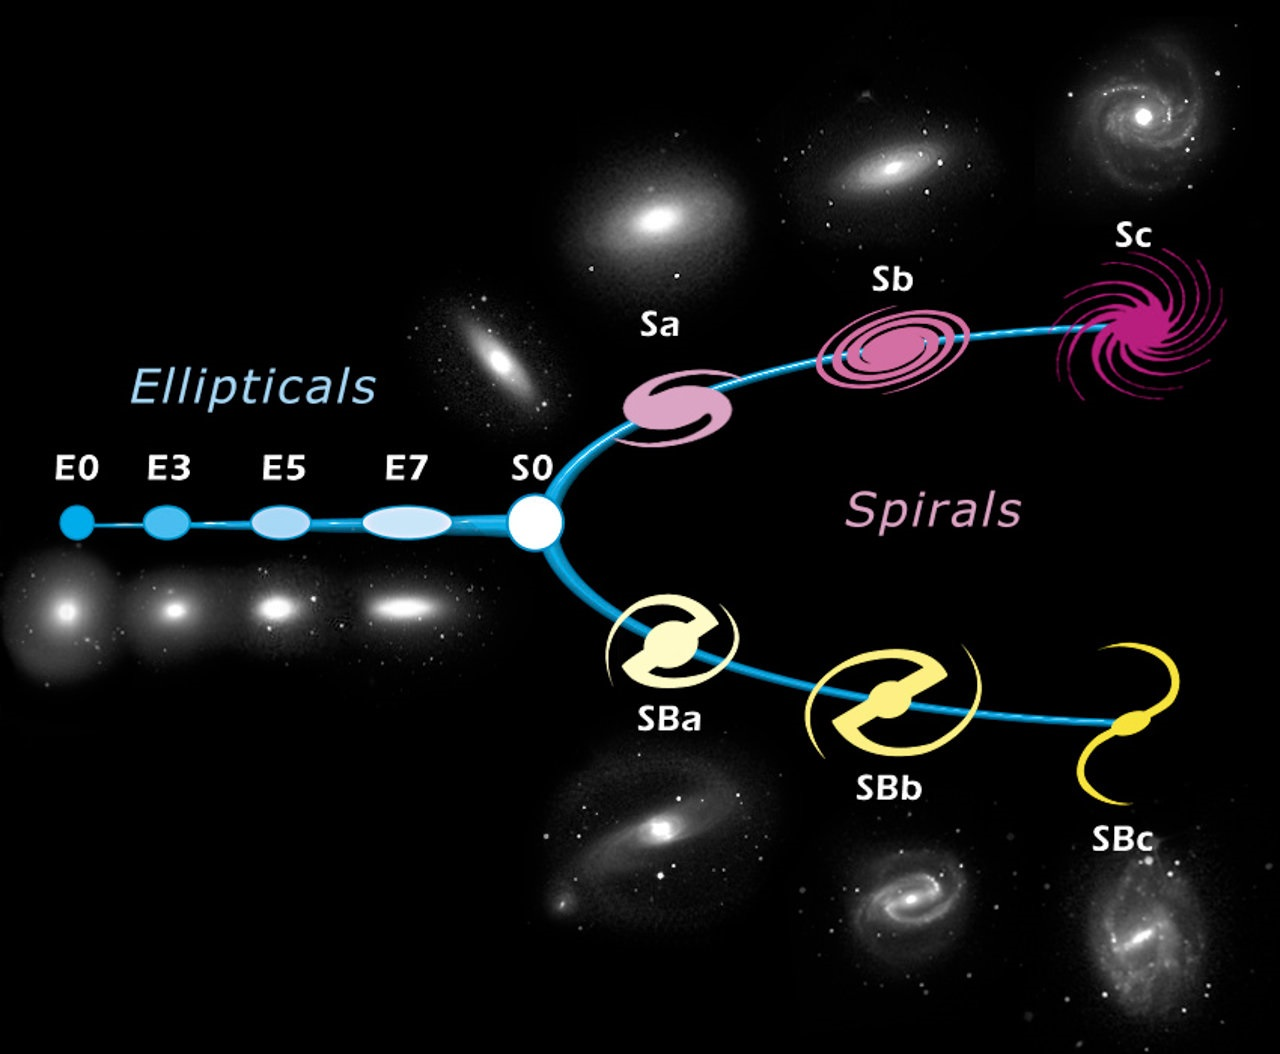
\includegraphics[width=0.6\textwidth]{introduction/hubble.jpg}
		\caption[The Hubble tuning-fork]{Hubble diagram (or tuning fork), showing the different morphology classifications of galaxies. Spirals exist on two sequences: barred and un-barred. The handle of the tuning folk contains ETGs, with S0s being the meeting point of all three sequences. Figure courtesy of http://spacetelescope.org.}
		\label{fig:Hubble}
	\end{figure}

	\begin{figure}
		\centering
		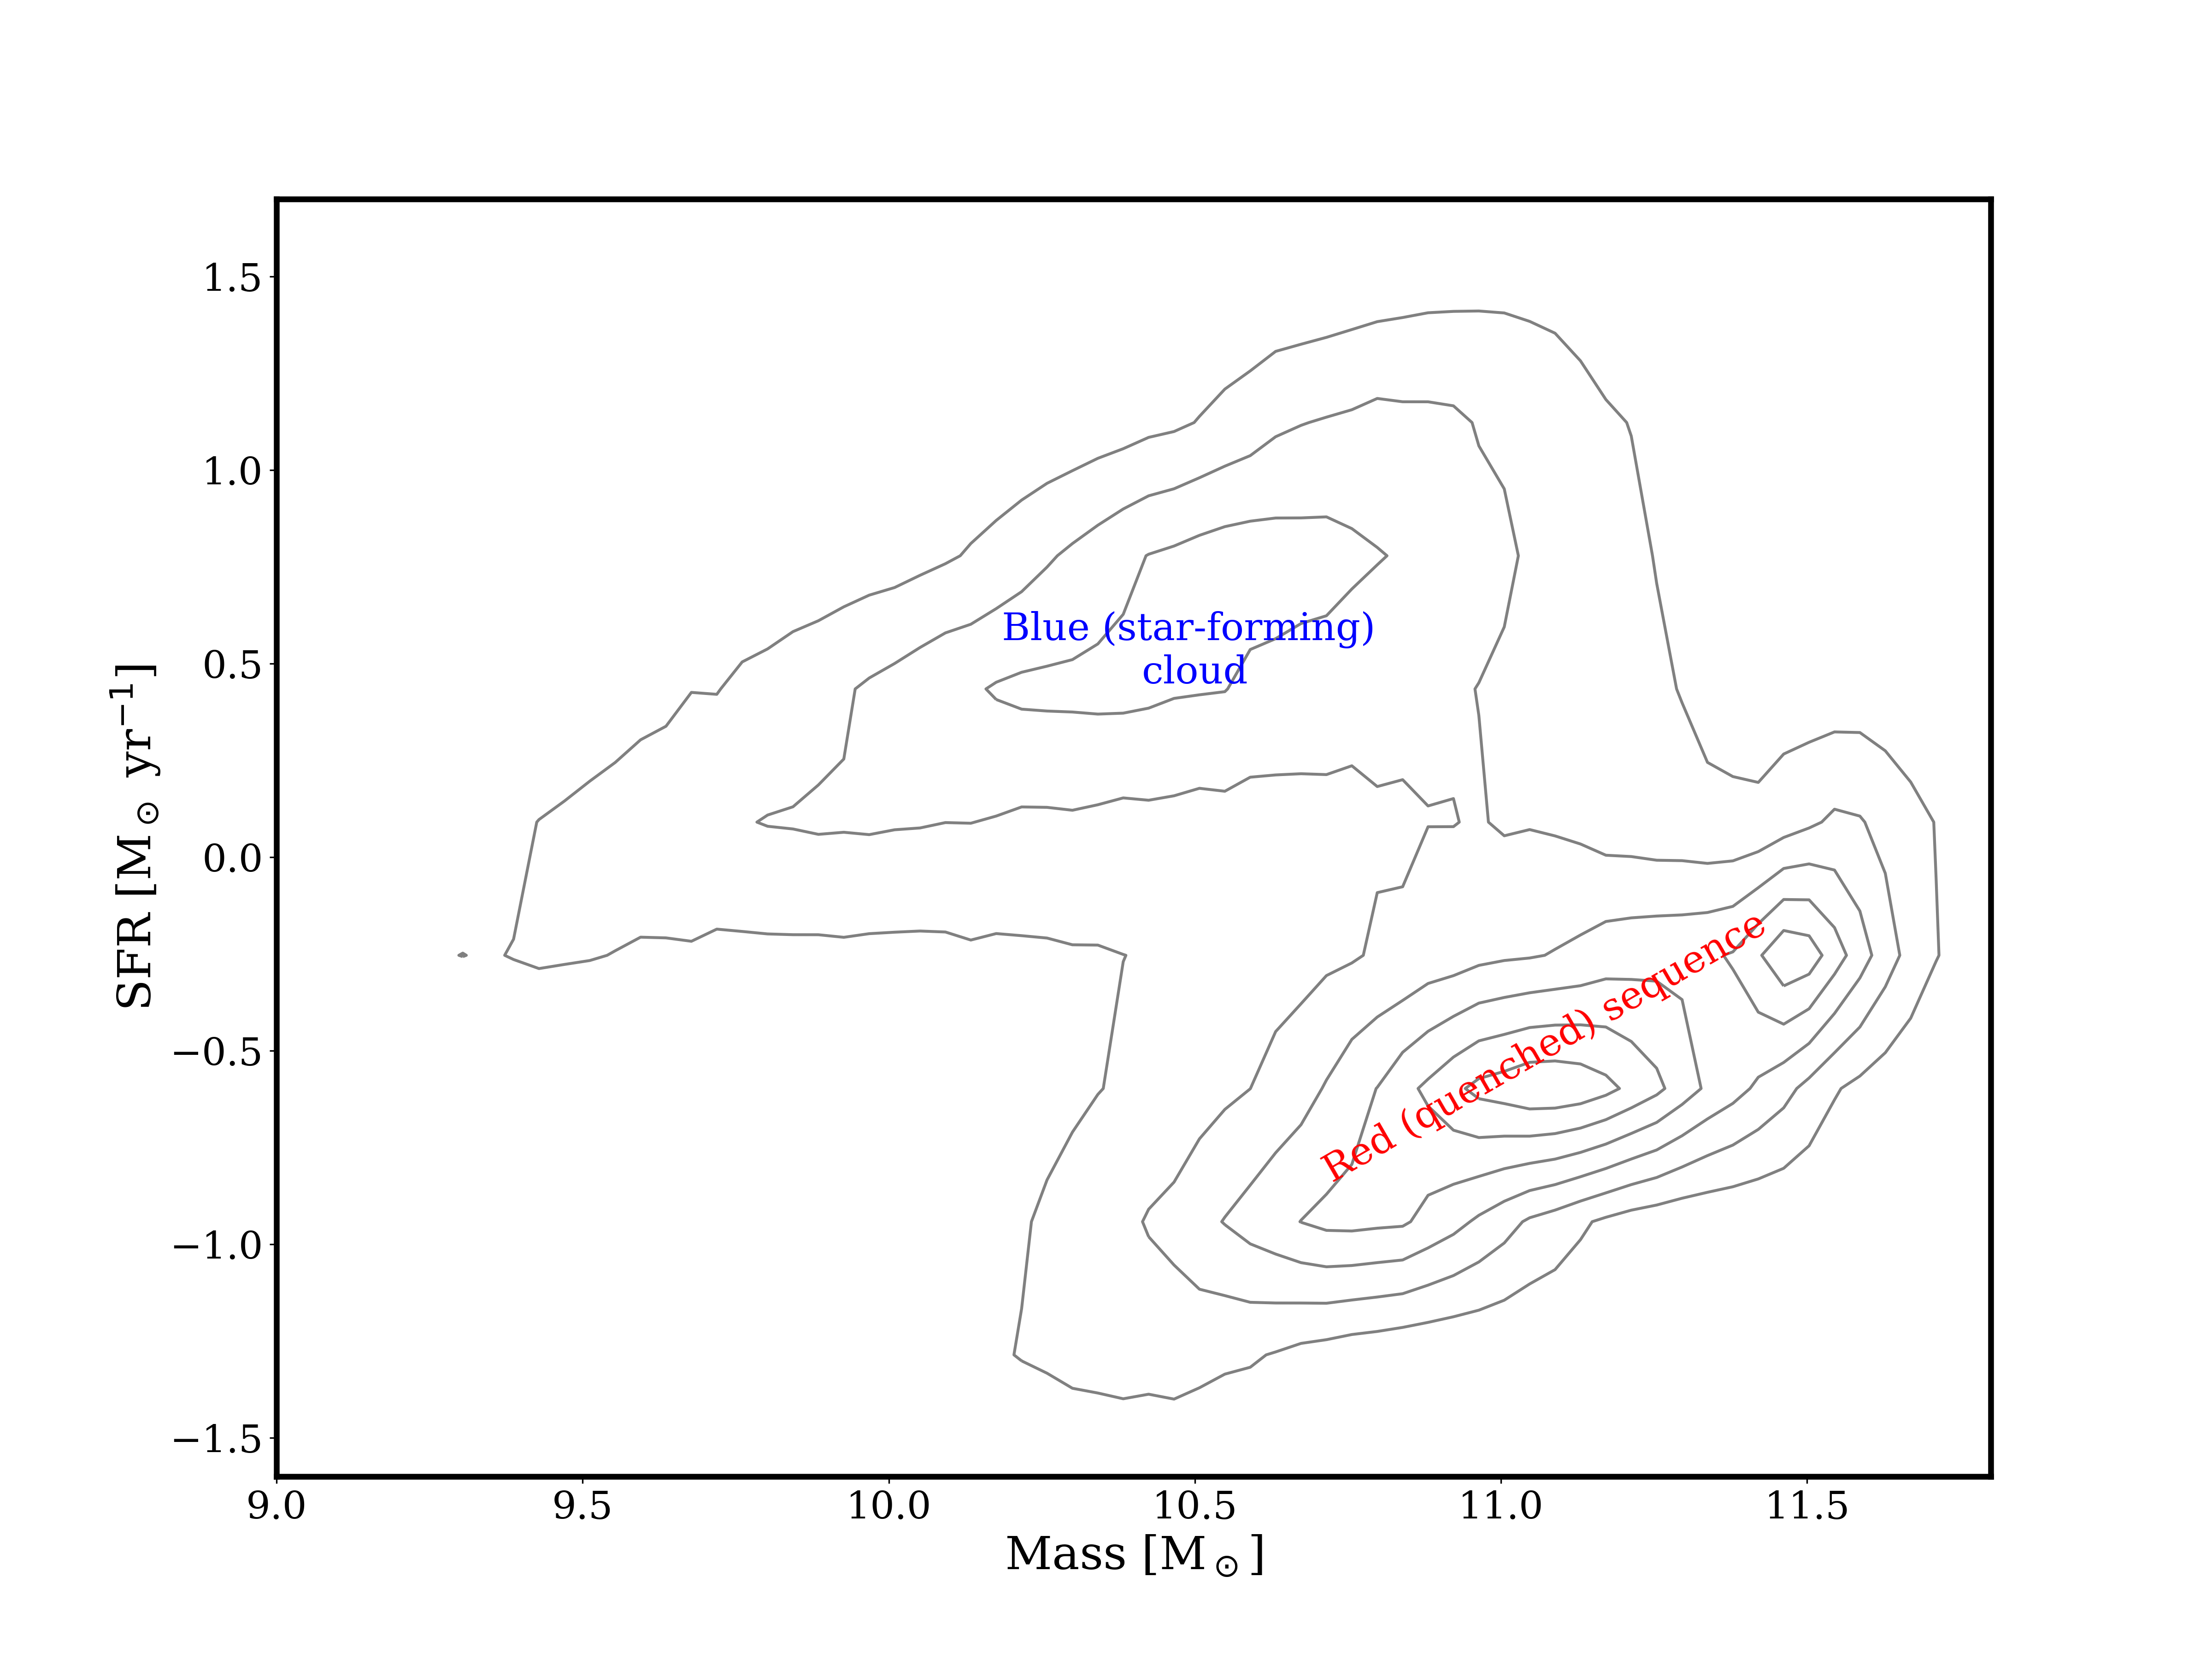
\includegraphics[width=0.7\textwidth]{introduction/sfMass.png}
		\caption[Star-formation rate--galaxy mass diagram]{The star-formation rate--mass plane for the MPA-JHU sample galaxies \citep{Kauffmann2003, Brinchmann2003, Salim2007} clearly showing the dichotomy between the blue cloud and red sequence galaxies.}
		\label{fig:ColourMass}
	\end{figure}

	\begin{figure}
		\centering
		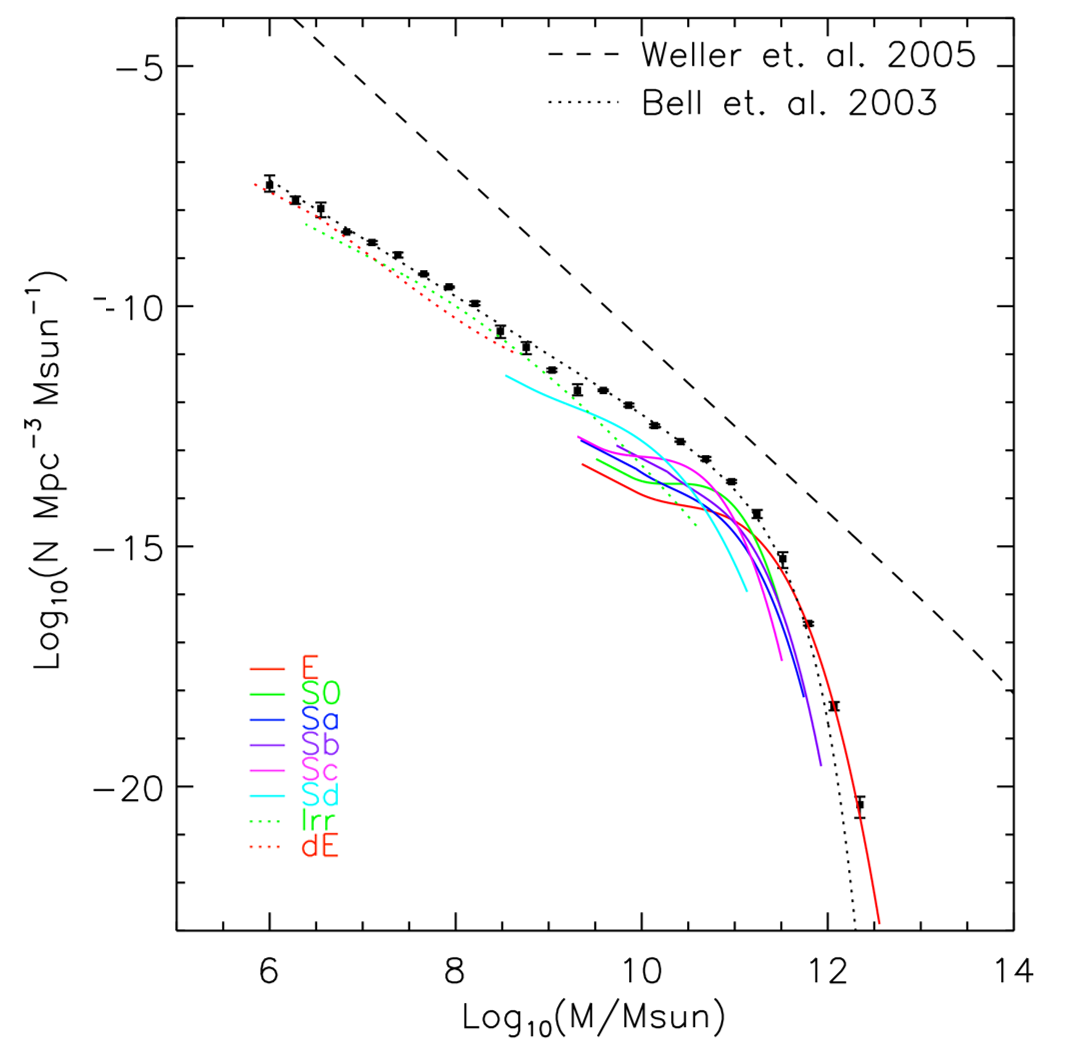
\includegraphics[width=.6\textwidth]{introduction/agnFeedback.png}
		\caption[Galaxy mass function]{Galaxy mass function. The coloured lines (both solid and dotted) show spline fits by Hubble type (ellipticals are shown by the solid red line), while the dashed black line shows the expected dark matter halo mass function \citep{Weller2005} and the dotted line is the Schechter function fit to all galaxies \citep{Bell2003}. Figure courtesy of \citet{Read2005}.}
		\label{fig:massSuppression}
	\end{figure}

	Given their low star formation rates, ETGs are dominated by old stars, while spirals are dominated by young stars. Understanding the reasons for this dichotomy is a major quest of modern astrophysics. ETGs are often the most massive galaxies, so they clearly must have undergone substantial star formation in their early history, that has now stopped. They either must have run out of fuel for forming stars or have experienced (and be experiencing) processes preventing star formation (commonly known as "quenching"). Many have been observed to contain at least some Col.\,(atomic and/or molecular) gas \citep[e.g.][]{Lees1991}, the material from which stars are formed. This seems to favor the latter. The reservoirs are, however, significantly smaller than in LTGs. Without this quenching of star formation, we should expect the galaxy mass function -- number density profile of galaxies shown in Fig.\,\ref{fig:massSuppression} to follow that of dark matter haloes, assuming pure hierarchical growth of overdensities (dashed line in Fig.\,\ref{fig:massSuppression}). Clearly, star-formation is being suppressed at both the high-mass and the low-mass end.

	\begin{figure}
		\centering
		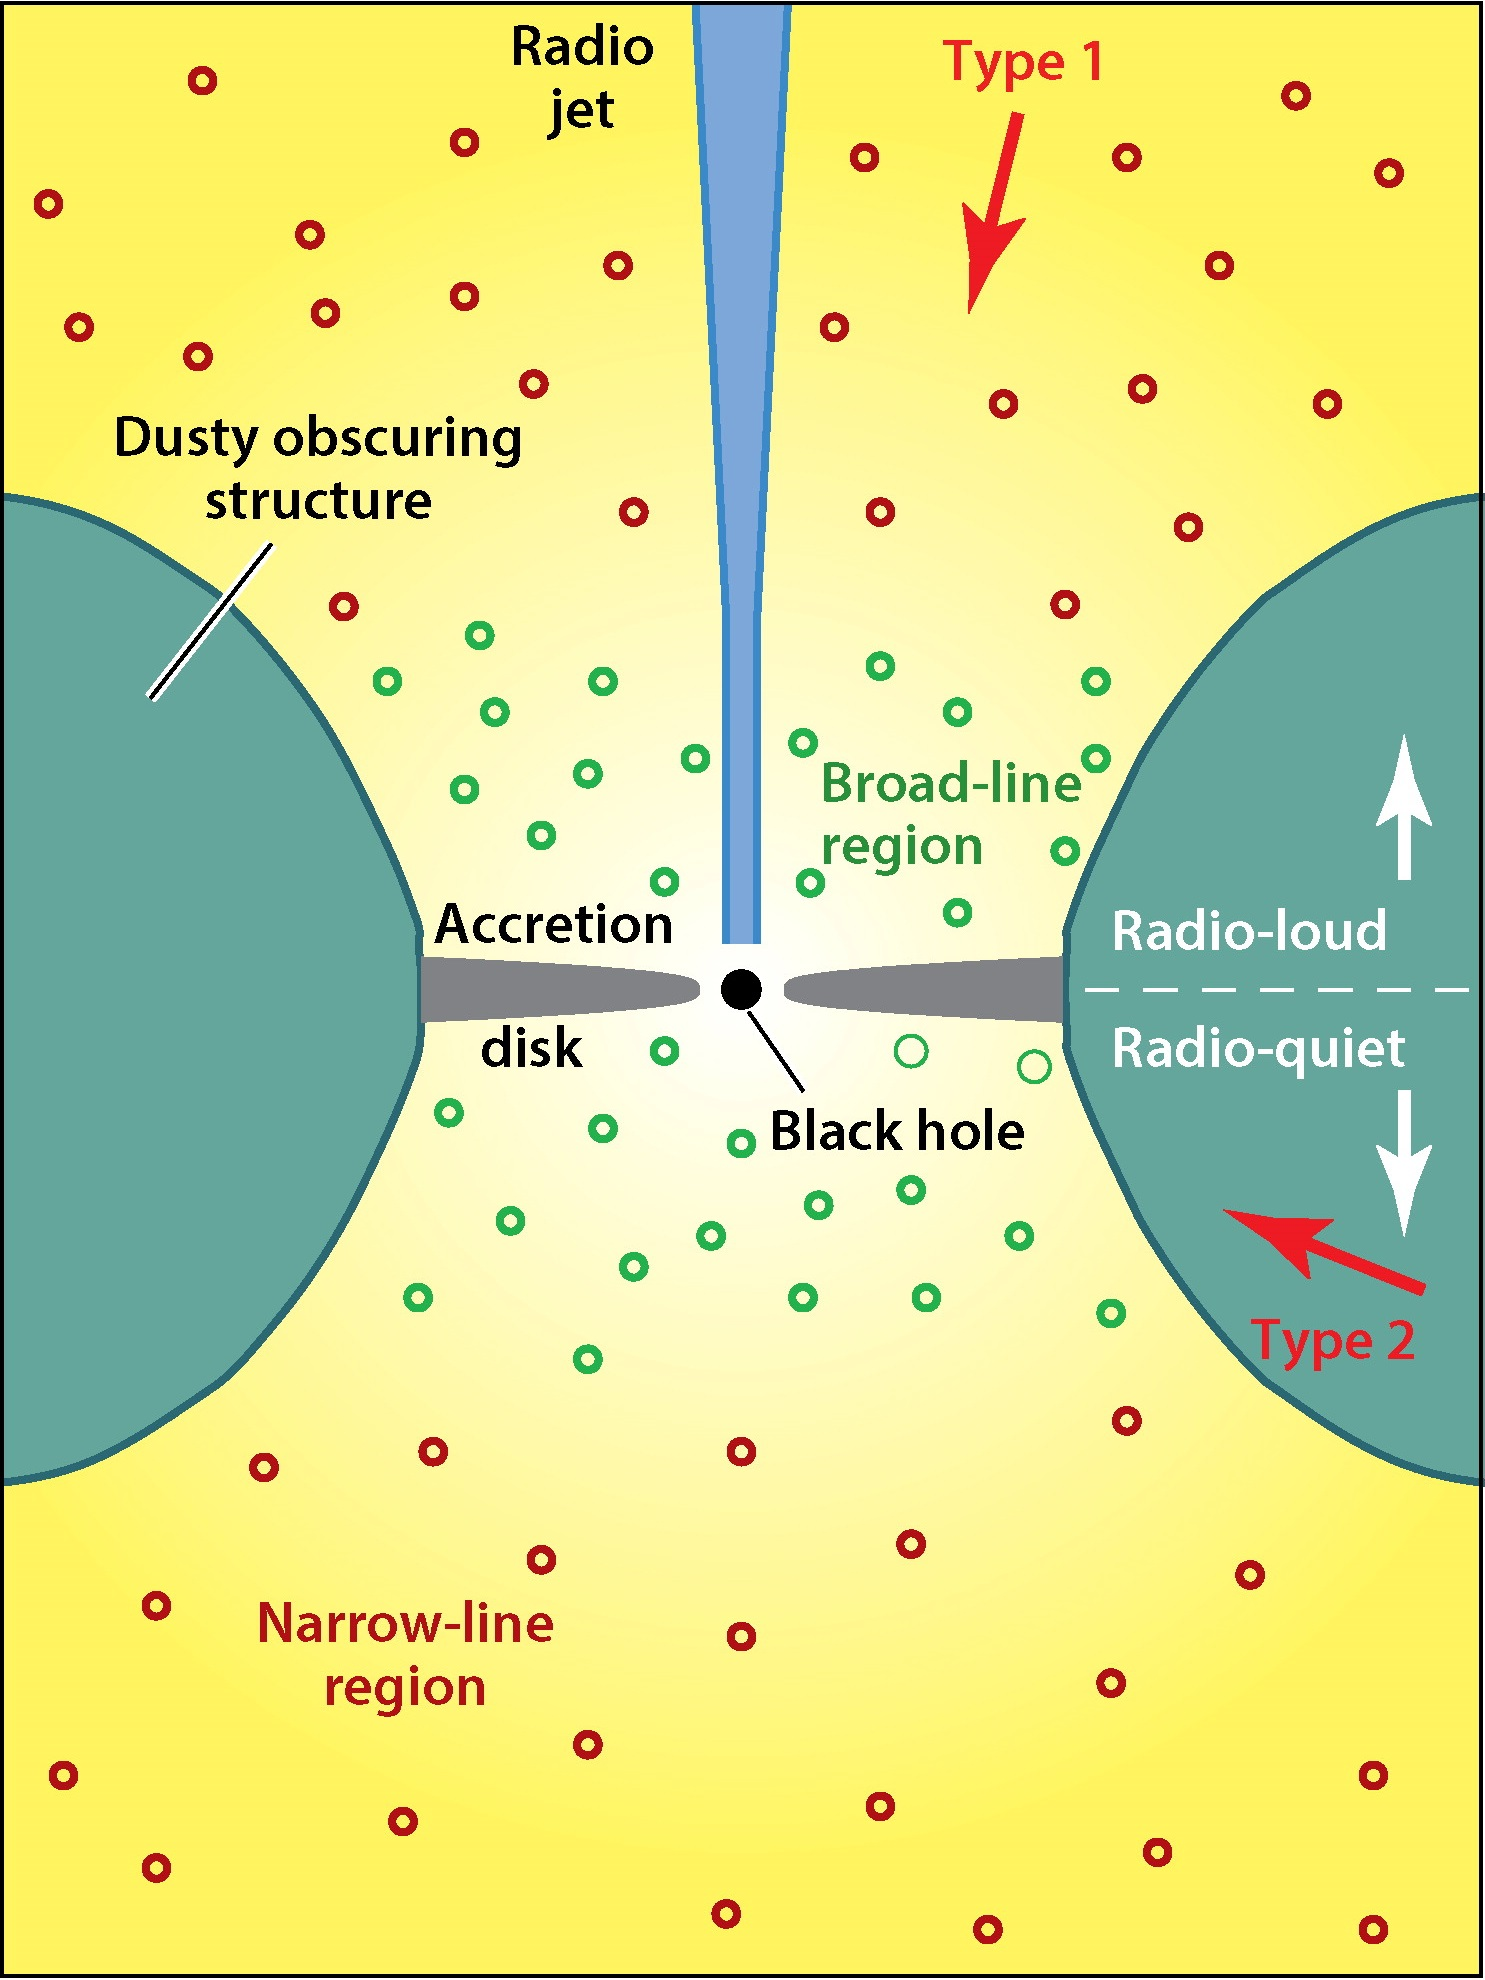
\includegraphics[width=.5\textwidth]{introduction/unifiedAGN.jpeg}
		\caption[Schematic of unified model of AGN]{Schematic of the unified model of AGN. The primary source of radiation is the accretion disc, which in turn ionises both the broad-line and narrow-line regions. A dust torus obscures side-on views (Type 2 AGN), while a jet sometimes emerges from the poles of the disc. Figure courtesy of \citet{Heckman2014}.}
		\label{fig:UnifiedAGN}
	\end{figure}

	Many studies now point to the fact that most (if not all) galaxies contain a super-massive black hole at their centre \citep[e.g.][]{Kormendy2013a}. There are tight correlations (known as scaling relations) between the properties of the central black holes and those of the host galaxies, despite orders of magnitude differences between the spheres of gravitational influence of the black holes and the sizes of the host galaxies \citep[e.g.][]{Gudehus1973, Faber1976, Ferrarese2000, Gebhardt2000}. 

	It is also seen that many galaxies contain a bright point source at their centre. These are known as active galactic nuclei (AGN), and in extreme cases (quasars) they can completely outshine the total starlight of the host galaxy. AGN are understood to be the result of the accretion of  inter-stellar matter (known as the inter-stellar medium; ISM) onto the central black hole \citep[e.g.][]{Lynden-Bell1969}, and the energy released by the AGN is generally invoked to explain the galaxy--black hole scaling relationships \citep[e.g.][]{Raimundo2010} as well as the quenching of star formation in (massive) ETGs \citep[e.g.][]{Croton2006, Somerville2008}. This process is known as AGN feedback and appears to be required by current numerical simulations and semi-analytic models to successfully reproduce the observed properties of massive galaxies \citep[e.g.][]{Kauffmann2000, Granato2004, DiMatteo2005, Springel2005, Bower2006, Croton2006, Hopkins2006, Ciotti2010, Scannapieco2012}. The exact fraction of galaxies that contain an AGN varies depending on the method employed to identify the AGN, but it is strongly mass dependent, with more massive galaxies more likely to contain an AGN \citep[e.g.][]{Kauffmann2003a}.

	AGN are varied, but much work has been done on a single unified model where the differences between individual galaxies can be explained by different orientations of the AGN. The unified model by \citet{Antonucci1993} describes AGN as made up of up to five components or regions surrounding the central black hole. (i) Immediately around the black hole is an accretion disc. Surrounding this is (ii) an obscuring dust torus, blocking side-on views of the black hole and accretion disc. Intense radiation from the accretion disc ionises (iii) the region immediately above and below the disc, which emits in the optical regime. The gas has very high orbital velocities ($\approx 5000 \, \mathrm{km \, s^{-1}}$) due to the proximity to the black hole, giving rise to characteristic broad lines and this region's name: broad-line region (BLR). The BLR is also obscured by the torus if viewed edge-on. Beyond this is (iv) the narrow-line region (NLR), an area of more sedate velocities ($\approx 200 \, \mathrm{km \, s^{-1}}$) and less ionised gas. Because of the shadow cast by the torus, the NLR sometimes appears as conical in shape \citep{Wilson1994}. Finally, a small proportion of AGN contain (v) jets of plasma traveling at relativistic speeds out from the poles of the accretion disc (the exact orientation of the jets may well also be dependent on the orientation of the spins of the black holes, though this remains unknown). The nature of the jets is explored in more detail below. AGN viewed side-on, with the black hole, accretion disc and BLR obscured by the torus are known as Type 2 AGN, while AGN viewed face-on, sometime viewing directly down the jet, are known as Type 1. A schematic of the unified model is shown in Fig.\,\ref{fig:UnifiedAGN}.


	Despite the unification of the many observed morphologies of AGN, it is becoming increasingly clear that AGN exist in two different modes, radiative and jet mode \citep[e.g.][]{Antonucci2012}, raising speculation about differing mechanisms and possibly fuel sources for each. More detail on both modes can be found in Section \ref{sec:AGN}. 


	Most galaxies also emit at radio frequencies. These galaxies are known as radio galaxies (RGs). Mostly this is attributed to star formation, which radiates due to free-free (thermal) emission from regions of ionised ISM (\ion{H}{ii} regions) and synchrotron emission from supernova remnants as relativistic electrons spiral along the strong magnetic field lines. Except in extreme star bursts, radio emission due to star formation is fairly low-level. Many AGN also emit in at radio frequencies due to synchrotron emission from the jets. Not considering star bursts, the brightest sources can be considered bona-fide detections of the AGN jets. However, distinguishing between star-formation and AGN jets can be difficult for fainter sources, though there is no consensus on where this transition should lie. Emission from AGN will always be from the centre of the galaxy (the location of the AGN) and extending out along the trajectory of the jets. However, \citet{Nyland2016} note that in the fainter centrally concentrated RGs, the radio emission is also consistent with circumnuclear star formation.

	There is broad consensus within the literature that the most powerful RGs ($\log P_\mathrm{1.4\, GHz}/(\mathrm{W \, Hz^{-1}}) \gtrsim 25.5$) are the product of gas-rich (wet) major mergers of galaxies (a major merger is defined as a merger of galaxies with a mass ratio smaller than 3:1). These AGN tend to be extremely luminous. Indeed, despite clearly containing a very powerful jet, they are mostly radiative mode AGN. These RGs form a very small minority of the RG population and hence are not representative. Indeed, \citet{Heckman2014} present evidence that most RGs are fueled through secular processes.

	This thesis will compare and contrast the stellar and ionised gas properties of RGs and radio-quiet ETGs. The rest of this chapter will thus cover the background required to study the RG population. Firstly, since RGs are primarily found in ETGs, the current understanding of ETGs will be reviewed. This is mostly a summary of the recent integral field spectroscopy (IFS) surveys including Atlas$^\text{3D}$, MaNGA, MASSIVE, SAMI and Califa, and can be considered as setting out of the control sample for later investigations (see Section \ref{sec:ETG}). Secondly, in Section \ref{sec:AGN}, a more detailed summary of the current state of our understanding of AGN will be presented, including RGs. Finally, the selection criteria of the sample used throughout this thesis will be described (Section \ref{sec:Sample}).

	Chapter \ref{cha:Data} gives details of the VIMOS and MUSE instruments, as well as the corresponding data reduction and analysis methods. Chapters \ref{cha:stellar} and \ref{cha:gas} cover the results, focusing on the stellar and ionised gas components, respectively, of the sample galaxies. Chapter \ref{cha:conclusion} presents a summary and conclusions. 

\section{Early-type Galaxies}
	\label{sec:ETG}
	Confusingly, due to historical reasons, there are several similar yet subtly different definitions of the LTG/ETG classes. Originally they were based purely on the morphology as seen in optical images: spirals were LTGs and ellipticals were ETGs, while there was debate about which class lenticular galaxies (S0s) belonged to. S0s appear disc-like like LTGs, but often contain older populations with less star formation like ETGs. This debate has confused the literature, with some taking the classification scheme to reflect the underlying stellar population and others the assumed method of dynamical support (rotation vs dispersion). In this thesis we use the stellar population view and as such include S0s within the ETG class.

	A useful morphological sub-classification within ETGs is the slope of the nuclear surface brightness profile. Some galaxies show a significant flattening of their surface brightness profile towards the centre of the galaxy (cored galaxies), whereas others show only a mild change (power-law galaxies). An example of each class is shown in Fig.\,\ref{fig:CorePower}. This is parametrised using a double power-law of the form
	\begin{align}
		\Sigma(R) = & \, \Sigma_\mathrm{b} \left(\frac{R_\mathrm{b}}{R}\right)^\gamma \left[\frac{1}{2} + \frac{1}{2}\left(\frac{R}{R_\mathrm{b}}\right)^\alpha\right]^{\frac{\gamma-\beta}{\alpha}} \, ,
		\label{eq:Nuker} \\
		\intertext{where $\gamma$ and $\beta$ control the inner and outer slope, respectively, $R_\mathrm{b}$ is the radius of the transition between the inner and out slopes, $\Sigma_\mathrm{b}$ is the surface brightness at $R_\mathrm{b}$ and $\alpha$ sets the speed of the transition. A galaxy is classifed using the derivative $\gamma'$:}
		\gamma' \equiv & \, - \left. \frac{\mathrm{d}\log I}{\mathrm{d} \log R} \right|_{R=R'} = - \frac{\gamma + \beta \left(\frac{R'}{R_\mathrm{b}}\right)^\alpha}{1 + \left(\frac{R'}{R_\mathrm{b}}\right)^\alpha}
	\end{align}
	evaluated at \textit{Hubble Space Telescope's (HST)} resolution limit of $R' = 0.1"$. A galaxy with $\gamma' \le 0.3$ is a considered a cored galaxy, while one with $\gamma' \ge 0.5$ is called a power-law (or `cuspy') galaxy. In the range $0.3 < \gamma' < 0.5$, galaxies are considered intermediate. High-resolution images have shown that cored galaxies typically have `boxy' isophotes, while power-law galaxies typically have `discy' isophotes \citep[e.g.][]{Lauer1995, Faber1997}. In addition, these are respectively thought to correspond to triaxial and oblate 3 dimensional shapes \citep[e.g.][]{Krajnovic2011, Krajnovic2013a, Krajnovic2013}.

	\begin{figure}
		\centering
		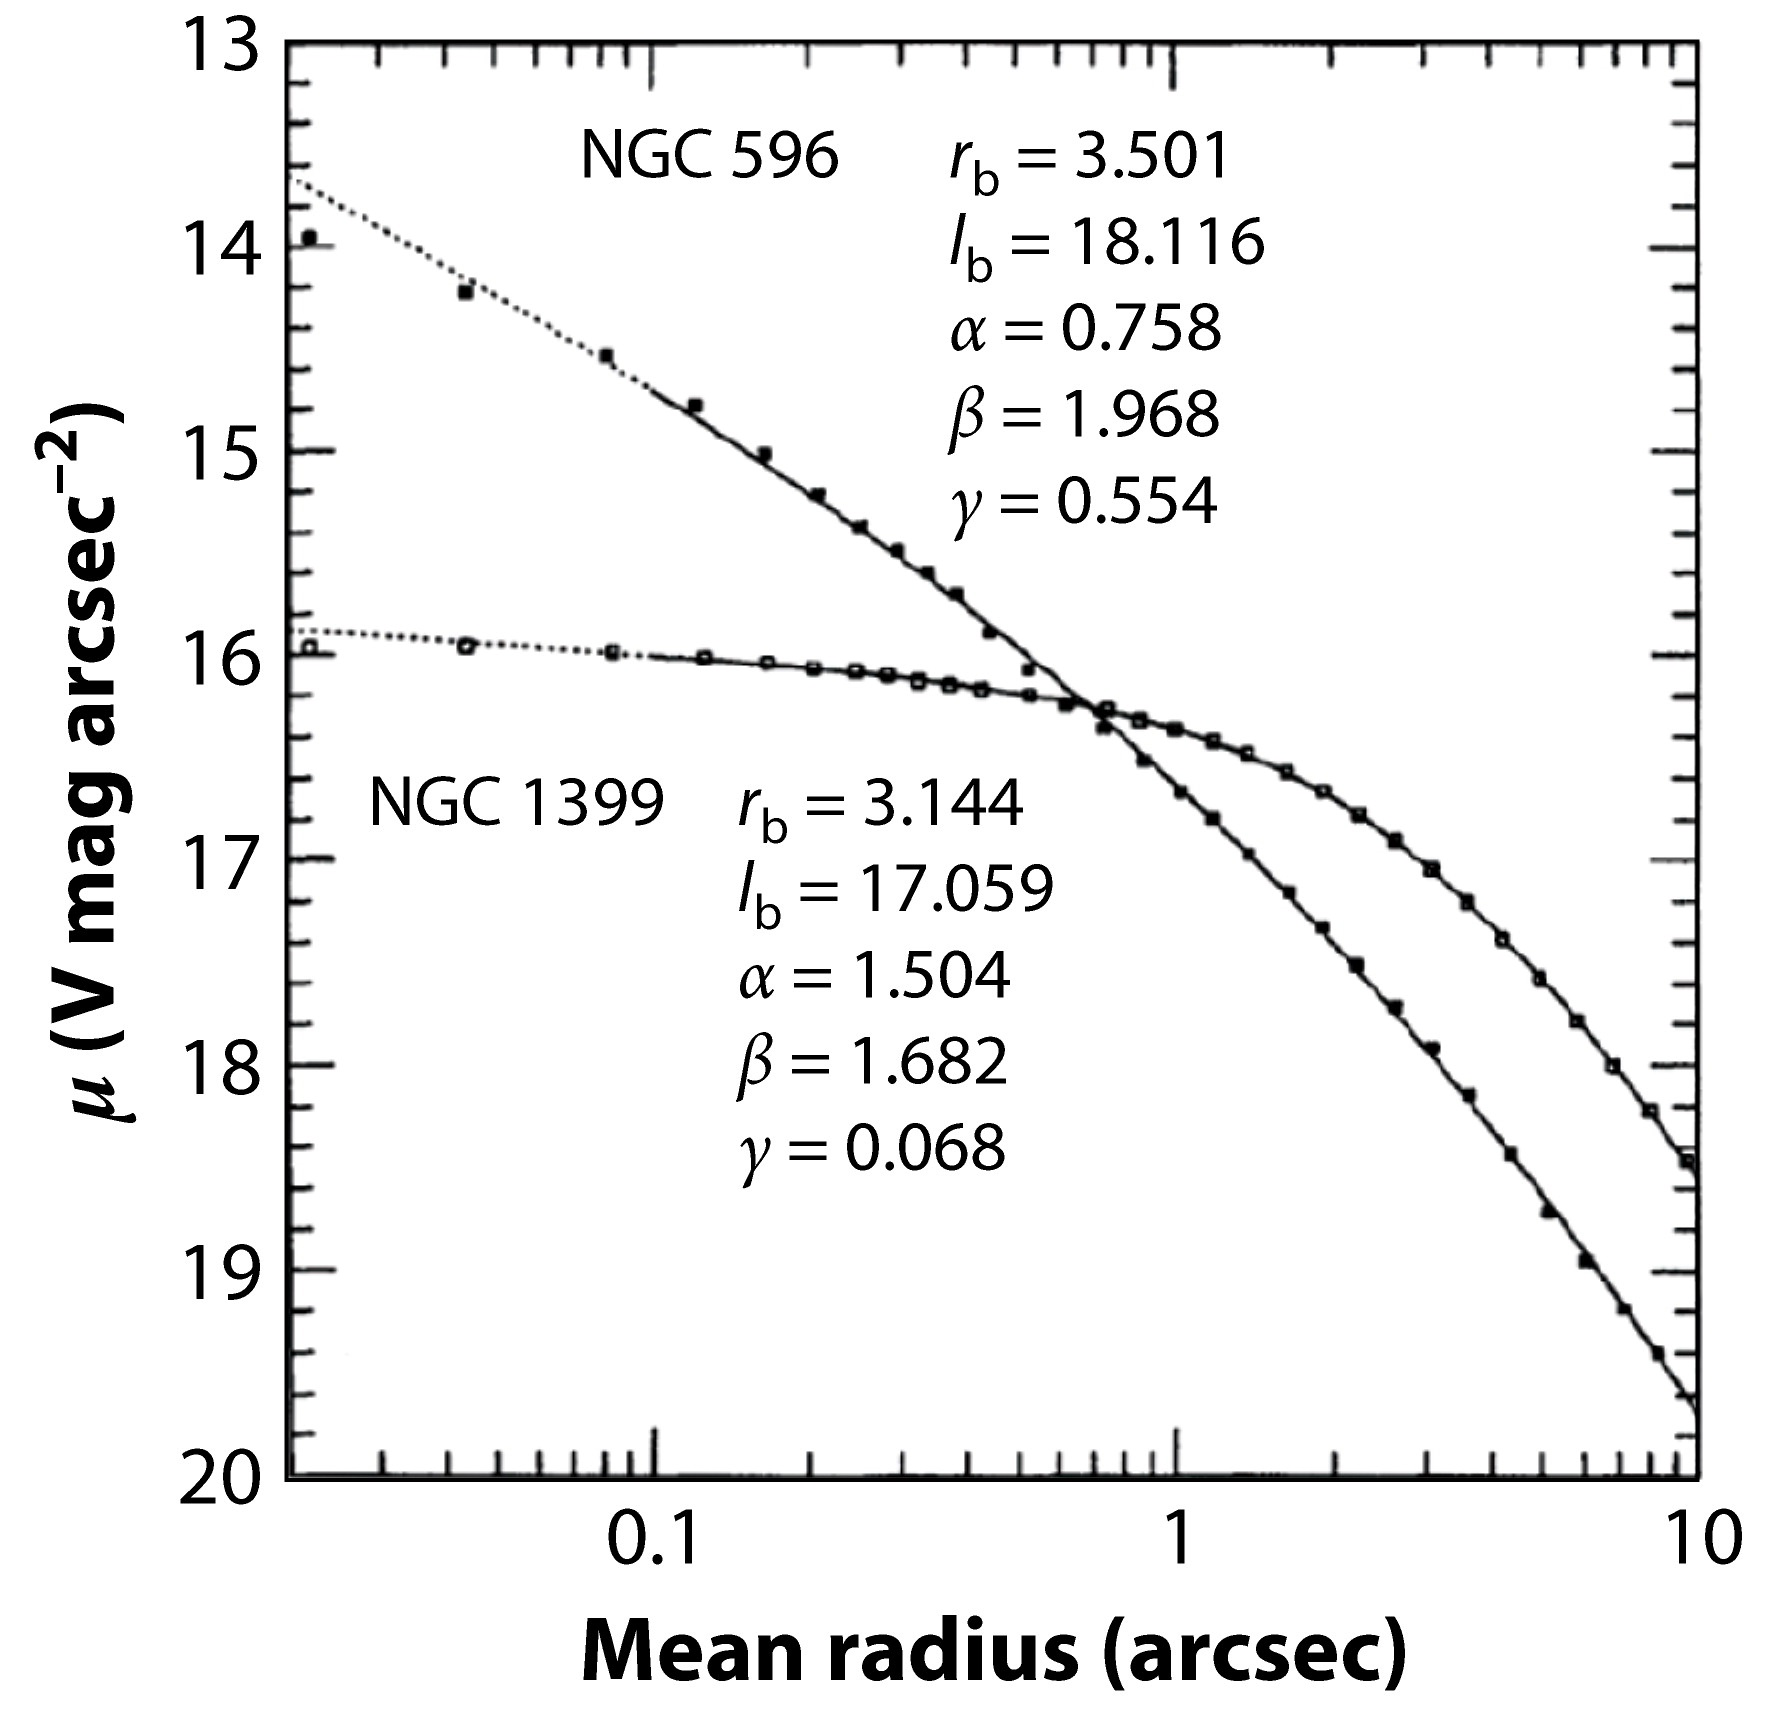
\includegraphics[width=0.5\textwidth]{introduction/exampleCorePower.jpeg}
		\caption[Example of cored and power-law surface brightness profile]{Examples of power-law (NGC 596) and cored (NGC 1399) surface brightness profiles. Both are fit with a double power law (Eq. \ref{eq:Nuker}), shown with the black lines. Both galaxies have similar outer slopes but dramatically different inner slopes. Figure courtesy of \citet{Lauer1995}.}
		\label{fig:CorePower}
	\end{figure}

	The Atlas$^\text{3D}$ survey \citep{Cappellari2011} found that morphologically categorising ETGs into ellipticals and S0s is misleading and does not not reflect underlying physical differences. Instead it used spatially-resolved stellar kinematics to classify ETGs into fast or slow rotators, depending on their value of $\lambda_R$ \citep{Emsellem2011}, where $\lambda_R$ is a parameter that quantifies a galaxy's specific angular momentum and is defined as
	\begin{align}
		\lambda_R \equiv & \frac{\langle R |V|\rangle}{\langle R \sqrt{V^2 + \sigma^2}\rangle} \, ,\\
		\intertext{where the angled brackets represent flux-weighted averages within a radius $R$, $V$ is the mean stellar velocity and $\sigma$ is the stellar velocity dispersion. For spatially-binned data:}
		\lambda_R = & \frac{\sum_{i=1}^{N} F_i R_i |V_i|}{\sum_{i=1}^{N} F_i R_i \sqrt{V_i^2 + \sigma_i^2}} \, ,
	\end{align}
	where $F_i$ is the flux of the $i^\text{th}$ bin, $R_i$ its distance from the centre and $V_i$ and $\sigma_i$ its mean stellar velocity and velocity dispersion, respectively. The sum is computed over all $N$ bins with a radius $R$. 

	The most recent definition of a slow rotator is
	\begin{equation}
		\lambda_\mathrm{R_e} < 0.08 + \frac{\epsilon}{4} \text{    and    } \epsilon < 0.4 \, ,
	\end{equation}
	where $\epsilon$ is the galaxy ellipticity and $\lambda_\mathrm{R_e}$ the value of $\lambda_R$ evaluated at the effective radius $\mathrm{R_e}$ \citep{Cappellari2016}. % Need to find original place this was defined (not just Michele's review).
	It is worth noting here that while most S0s are fast rotators and most slow rotators are ellipticals, the converses are not necessarily true: many ellipticals are fast rotators and some slow rotators are S0s. In fact the dichotomy is better reflected by the cored verse power-law morphologies, though \citet{Cappellari2016} notes that the kinematic classification scheme has the advantage that it is nearly inclination independent and can be measured at much lower spatial resolution. Having said that, the cases where the two classifications do not agree are often due to misclassified kinematics, such as counter-rotating stellar discs erroneously classified as slow rotators \citep[e.g.][]{Pinkney2003, Cappellari2005, Cappellari2007}. 

	Most slow rotators are massive, with stellar masses $M_\ast \gtrsim 10^{10.5} M_\odot$ and they dominate the high-mass end of the galaxy mass function, though fast rotators dominate in number by a factor of $\approx 7$ \citep[e.g.][]{Emsellem2011, Veale2017}. Fig.\,\ref{fig:SlowRotFrac} shows the change in the proportion of slow rotators as a function of stellar mass (for which $K$-band magnitude, $M_K$, is used as a proxy).


	\begin{figure}
		\centering
		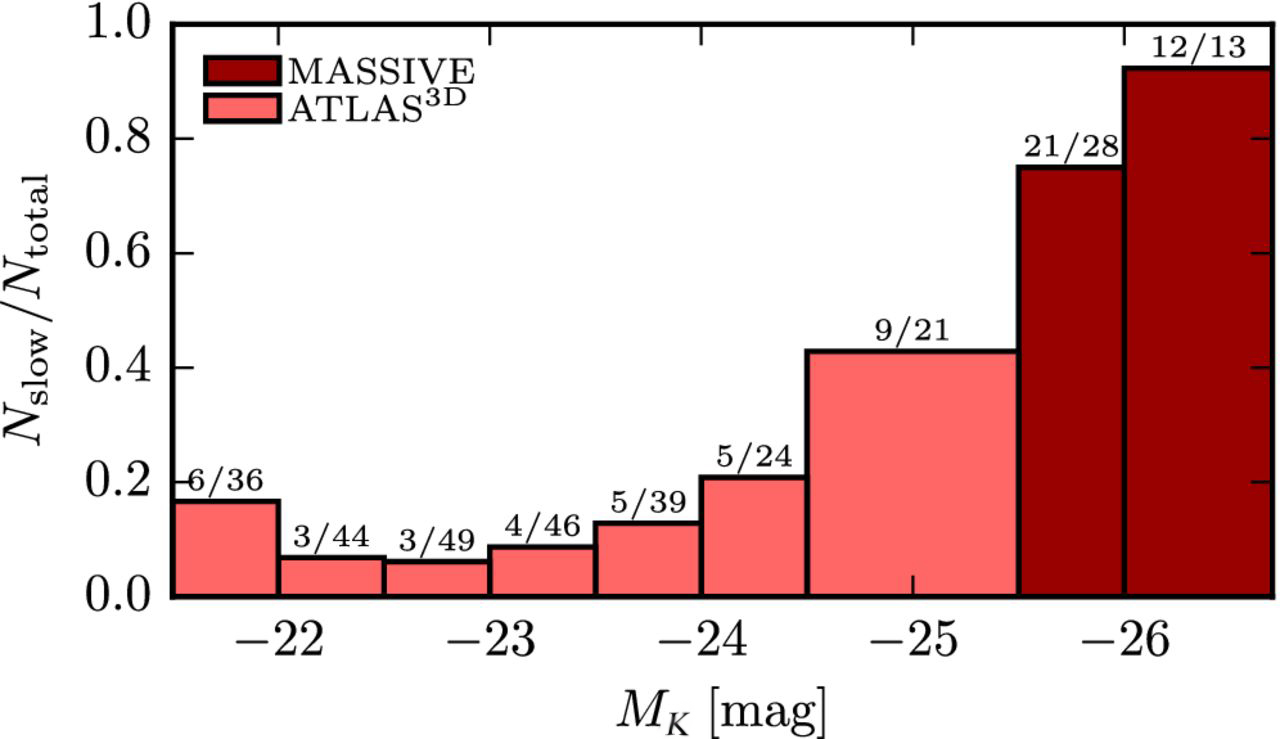
\includegraphics[width=0.8\textwidth]{introduction/slowRotFraction.jpeg}
		\caption[Proportion of slow rotating galaxies as a function of mass]{The fraction of slow rotators (within the total number of galaxies) as a function of total $K$-band magnitude ($M_K$), used as a proxy for total stellar mass. Figure courtesy of \citet{Veale2017}.}
		\label{fig:SlowRotFrac}
	\end{figure}

	Fast rotators reflect many properties of and have strikingly similar spatial distributions to spirals. Fast rotators have been shown to contain discs, and even very round objects can be shown to be face-on discs \citep[e.g.][]{Cappellari2013a, Weijmans2014}. They also have very similar bulge-to-disc ratios to spirals \citep{Krajnovic2013}. In Fig.\,\ref{fig:MassRe}, fast rotators form a parallel sequence to spiral galaxies.

	The discovery of the fast/slow-rotator scheme re-ignites the S0 debate and led the Atlas$^\text{3D}$ team to re-evaluate the Hubble sequence. In its place they proposed the Atlas$^\text{3D}$ comb (shown in Fig.\,\ref{fig:Atlas3Dcomb}; \citealt{Cappellari2011a}) where fast rotating ETGs form a parallel sequence to spirals in the scaling relationship (e.g.\ the galaxy mass--size plane; see Fig.\,\ref{fig:MassRe}), but share many properties such as stellar age and gas content with slow rotating ETGs. 

	\begin{figure}
		\centering
		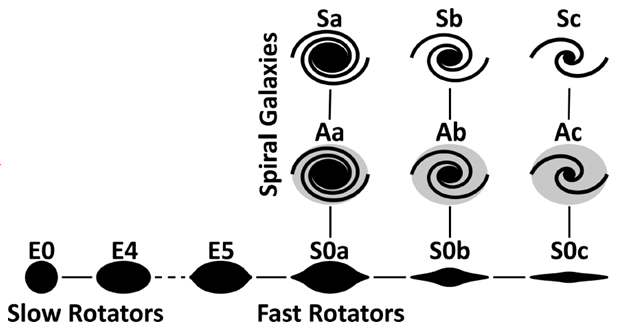
\includegraphics[width=0.8\textwidth]{introduction/Atlas3D_comb.png}
		\caption[The Atlas$^\text{3D}$ comb]{The Atlas$^\text{3D}$ comb, a replacement of the Hubble tuning fork (Fig.\,\ref{fig:Hubble}). ETGs (bottom row) form a parallel sequence to spirals in terms of the rotation and bulge-to-disc ratio. Solid lines show empirical continuity, while the dashed line represents the discontinuity between the fast and slow rotators. The intermediate `anemic' spirals, as classified by \citet{VandenBergh1976}, are included to demonstrate the continuous nature of the link between S0s and spirals. Figure courtesy of \citet{Cappellari2011a}.}
		\label{fig:Atlas3Dcomb}
	\end{figure}

	Since \citet{Sarzi2015} showed inner power-laws against be fragile to dry major mergers, cores are assumed to be markers that the galaxy has undergone such a merger. The near 1:1 correspondence between the slow/fast rotators and cored/power-law classifications shows that dry major mergers must also be responsible for forming slow rotators and changing the shapes of galaxies from oblate to triaxial.

	One useful test for a triaxial shape is misalignment between the kinematic (rotation) axis and the apparent morphological minor axis. For oblate structures, the two should align within $\approx 5\degree$, but for triaxial structures they can have any misalignment \citep[e.g.][]{Contopoulos1956, Stark1977, Statler1987}. This is seen in Fig.\,\ref{fig:Misalignment}, where regular rotators have aligned photometric and kinematic position angles, and non-regular rotators have any value for the misalignment and low ellipticities. This supports the argument for fast rotators to be axisymmetric oblates, while slow rotators are triaxial, but fairly spherical.

	\begin{figure}
		\centering
		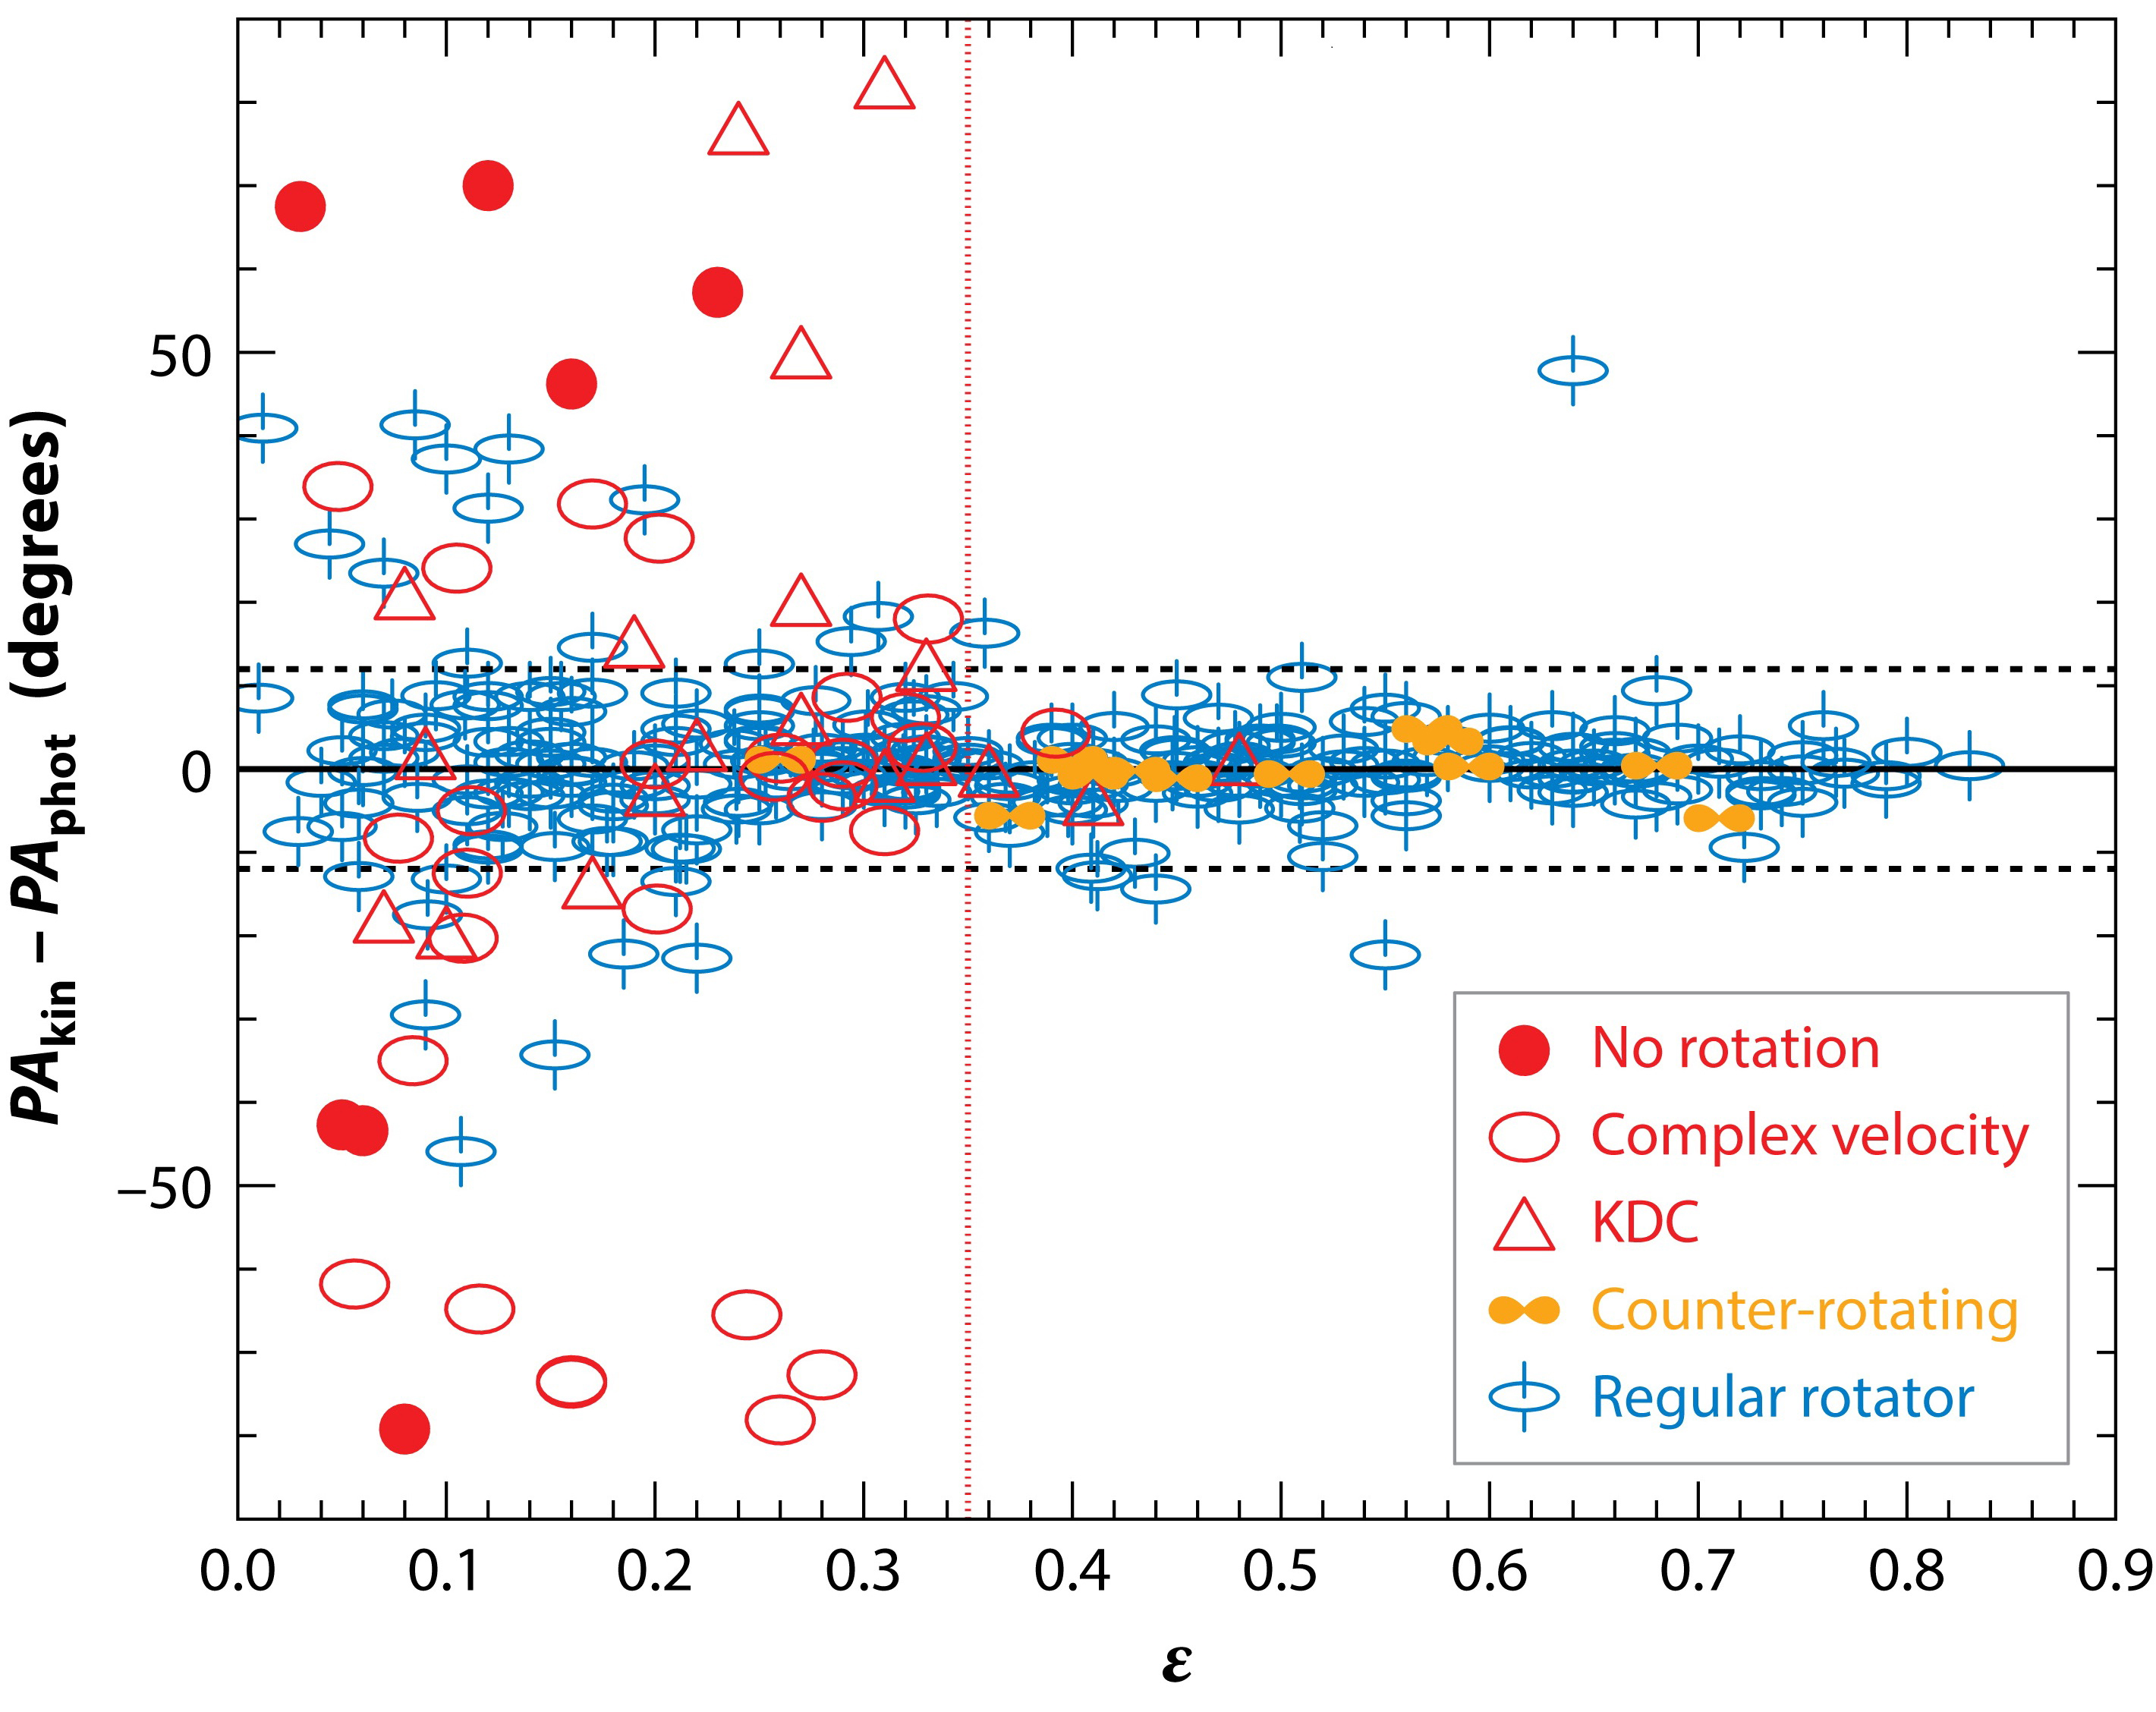
\includegraphics[width=0.7\textwidth]{introduction/misalignment.jpg}
		\caption[The kinematic--photometric misalignment in slow rotators]{Misalignment of the position angles (PAs) of galaxies in the Atlas$^\text{3D}$ and SAMI pilot surveys. Figure courtesy of \citet{Cappellari2016}. KDC is the abbreviation of kinematically decoupled cores.}
		\label{fig:Misalignment}
	\end{figure}

	Fig.\,\ref{fig:MassRe} shows the parallel sequence of S0s to spiral galaxies represented in the Atlas$^\text{3D}$ comb on the galaxy mass--size plane. Galaxies are thought to evolve by gas accretion maintaining roughly constant radii. This increases the bulge-to-mass ratio, moving accreting galaxies from right to left along the fast rotator/spiral section of the Atlas$^\text{3D}$ comb. Major dry mergers transform the galaxies into slow rotators \citep[e.g.][]{Bendo2000} with similar properties to those observed by Atlas$^\text{3D}$ \citep[e.g.][]{Jesseit2007, Jesseit2009}. After this, galaxies increase in mass due to continuous minor mergers \citep[e.g.][]{DeLucia2007, Genel2008, Feldmann2010, Oser2010, Feldmann2011, Hirschmann2012}. This moves the galaxy from the lower-centre to the upper-right of Fig.\,\ref{fig:MassRe}. 

	\begin{figure}
		\centering
		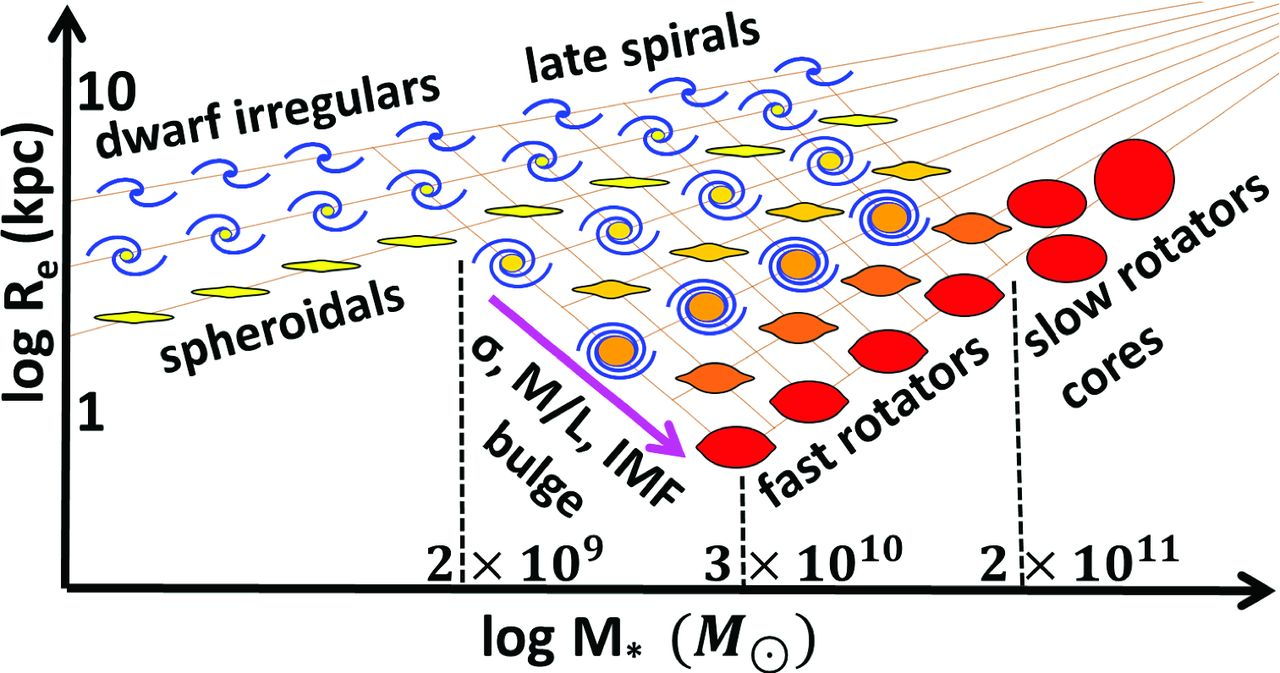
\includegraphics[width=0.7\textwidth]{introduction/mass_Re.jpg}
		\caption[The galaxy mass--size plane]{Galaxy mass--size plane, clearly showing the parallel sequences of S0s and spirals represented by in Atlas$^\text{3D}$ comb. Figure courtesy of \citet{Cappellari2013a}.}
		\label{fig:MassRe}
	\end{figure}

	Atlas$^\text{3D}$ also found a raft of kinematic substructures or features. These were split into five categories, a-e (examples shown in Fig.\,\ref{fig:EgSubstructure}), with a sixth category, f, containing unclassifiable objects \citep{Krajnovic2011}. These are mostly based on the results from the \textsc{kinemetry} routine\footnote{\url{http://davor.krajnovic.org/idl/}}\citep{Krajnovic2006}, which parametrises the stellar velocity map with a Fourier decomposition. The best-fitting ellipse is determined by minimizing all Fourier coefficients up the 3rd coefficient, $k_3$, except for the cosine term. Deviations from the cosine law are then represented by the $k_5$ harmonic \citep{Krajnovic2006}. Regular rotators (RRs; or galaxies that are well described by the cosine law) are defined as $\langle k_5/k_1 \rangle < 0.04$, which is based on the mean uncertainty of $k_5/k_1$ of $\approx 0.03$ for all Atlas$^\text{3D}$ galaxies. All other galaxies are classed as non-regular rotators (NRRs). While the RR/NRR classifications broadly reflect the fast/slow rotator classification, they should not be taken to have the same meaning. 

	Various kinematic features were also observed across the Atlas$^\text{3D}$ sample \citep{Krajnovic2011}. Galaxies are flagged as having
	\begin{itemize}
		\item \textbf{No feature (NF)}, if the position angle of the best-fit ellipse, $PA_\mathrm{kin}$, is constant with radius.
		\item \textbf{Double maxima (2M)}, if the radial profile of $k_1$ rises to a local maximum followed by a fall and another subsequent rise. The outer maximum is usually larger than the inner one. 
		\item \textbf{Kinematic twist (KT)}, if $PA_\mathrm{kin}$ varies smoothly with an amplitude of at least 10$\degree$. 
		\item \textbf{Kinematically decoupled/distinct core (KDC)}, if there is an abrupt change of $PA_\mathrm{kin}$ by more than 30$\degree$ and $k_1$ drops to near zero in the transition region. \textbf{Counter-rotating cores (CRCs)} are a special case where the change of $PA_\mathrm{kin}$ is about 180$\degree$.
		\item \textbf{Low velocities (VL)}, if $k_1 < 5 \, \mathrm{km \, s^{-1}}$, below the threshold of \textsc{kinemetry} to establish the ellipse parameters. These galaxies can be considered as non-rotating.
		\item \textbf{Double $\mathrm{\sigma}$ (2$\mathrm{\sigma}$)}, if there are two off-centre but symmetric peaks in the stellar velocity dispersion. These galaxies are understood to contain two counter-rotating discs. 
	\end{itemize}
	Examples of each of the features above can be seen in Fig.\,1 of \citet{Krajnovic2011}. The matching of these features with substructure categories is given in Table \ref{tab:KinGroups}, which also lists the total number of galaxies in each category in the Atlas$^\text{3D}$ sample. 

	\begin{table}
		\centering
	\begin{threeparttable}
		\caption{Kinematic groups defined by Atlas$^\text{3D}$.}
		\label{tab:KinGroups}
		\begin{tabular}{c l l}
			\hline
			\hline
			Group 	& N$_\text{gals}$ & Features \\
			\hline
			a 		& 7			& NRR/LV \\
			b 		& 12		& NRR/NF \\
			c 		& 19		& NRR/KDC, NRR/CRC, RR/CRC \\
			d 		& 11		& NRR/2$\mathrm{\sigma}$, RR/2$\mathrm{\sigma}$ \\
			e 		& 209		& RR/NF, RR/2M, RR/KT \\
			f 		& 2			& Unclassified \\
			\hline
			\hline
		\end{tabular}
		\begin{tablenotes}
		\footnotesize
		\note Col.\,1: Kinematic group. Col.\,2: number of galaxies from the Atlas$^\text{3D}$ sample out of 260. Col.\,3: kinematic features defining the group. Table reproduced from \citet{Krajnovic2011}.
		\end{tablenotes}
	\end{threeparttable}
	\end{table}

	\begin{figure}
		\centering
		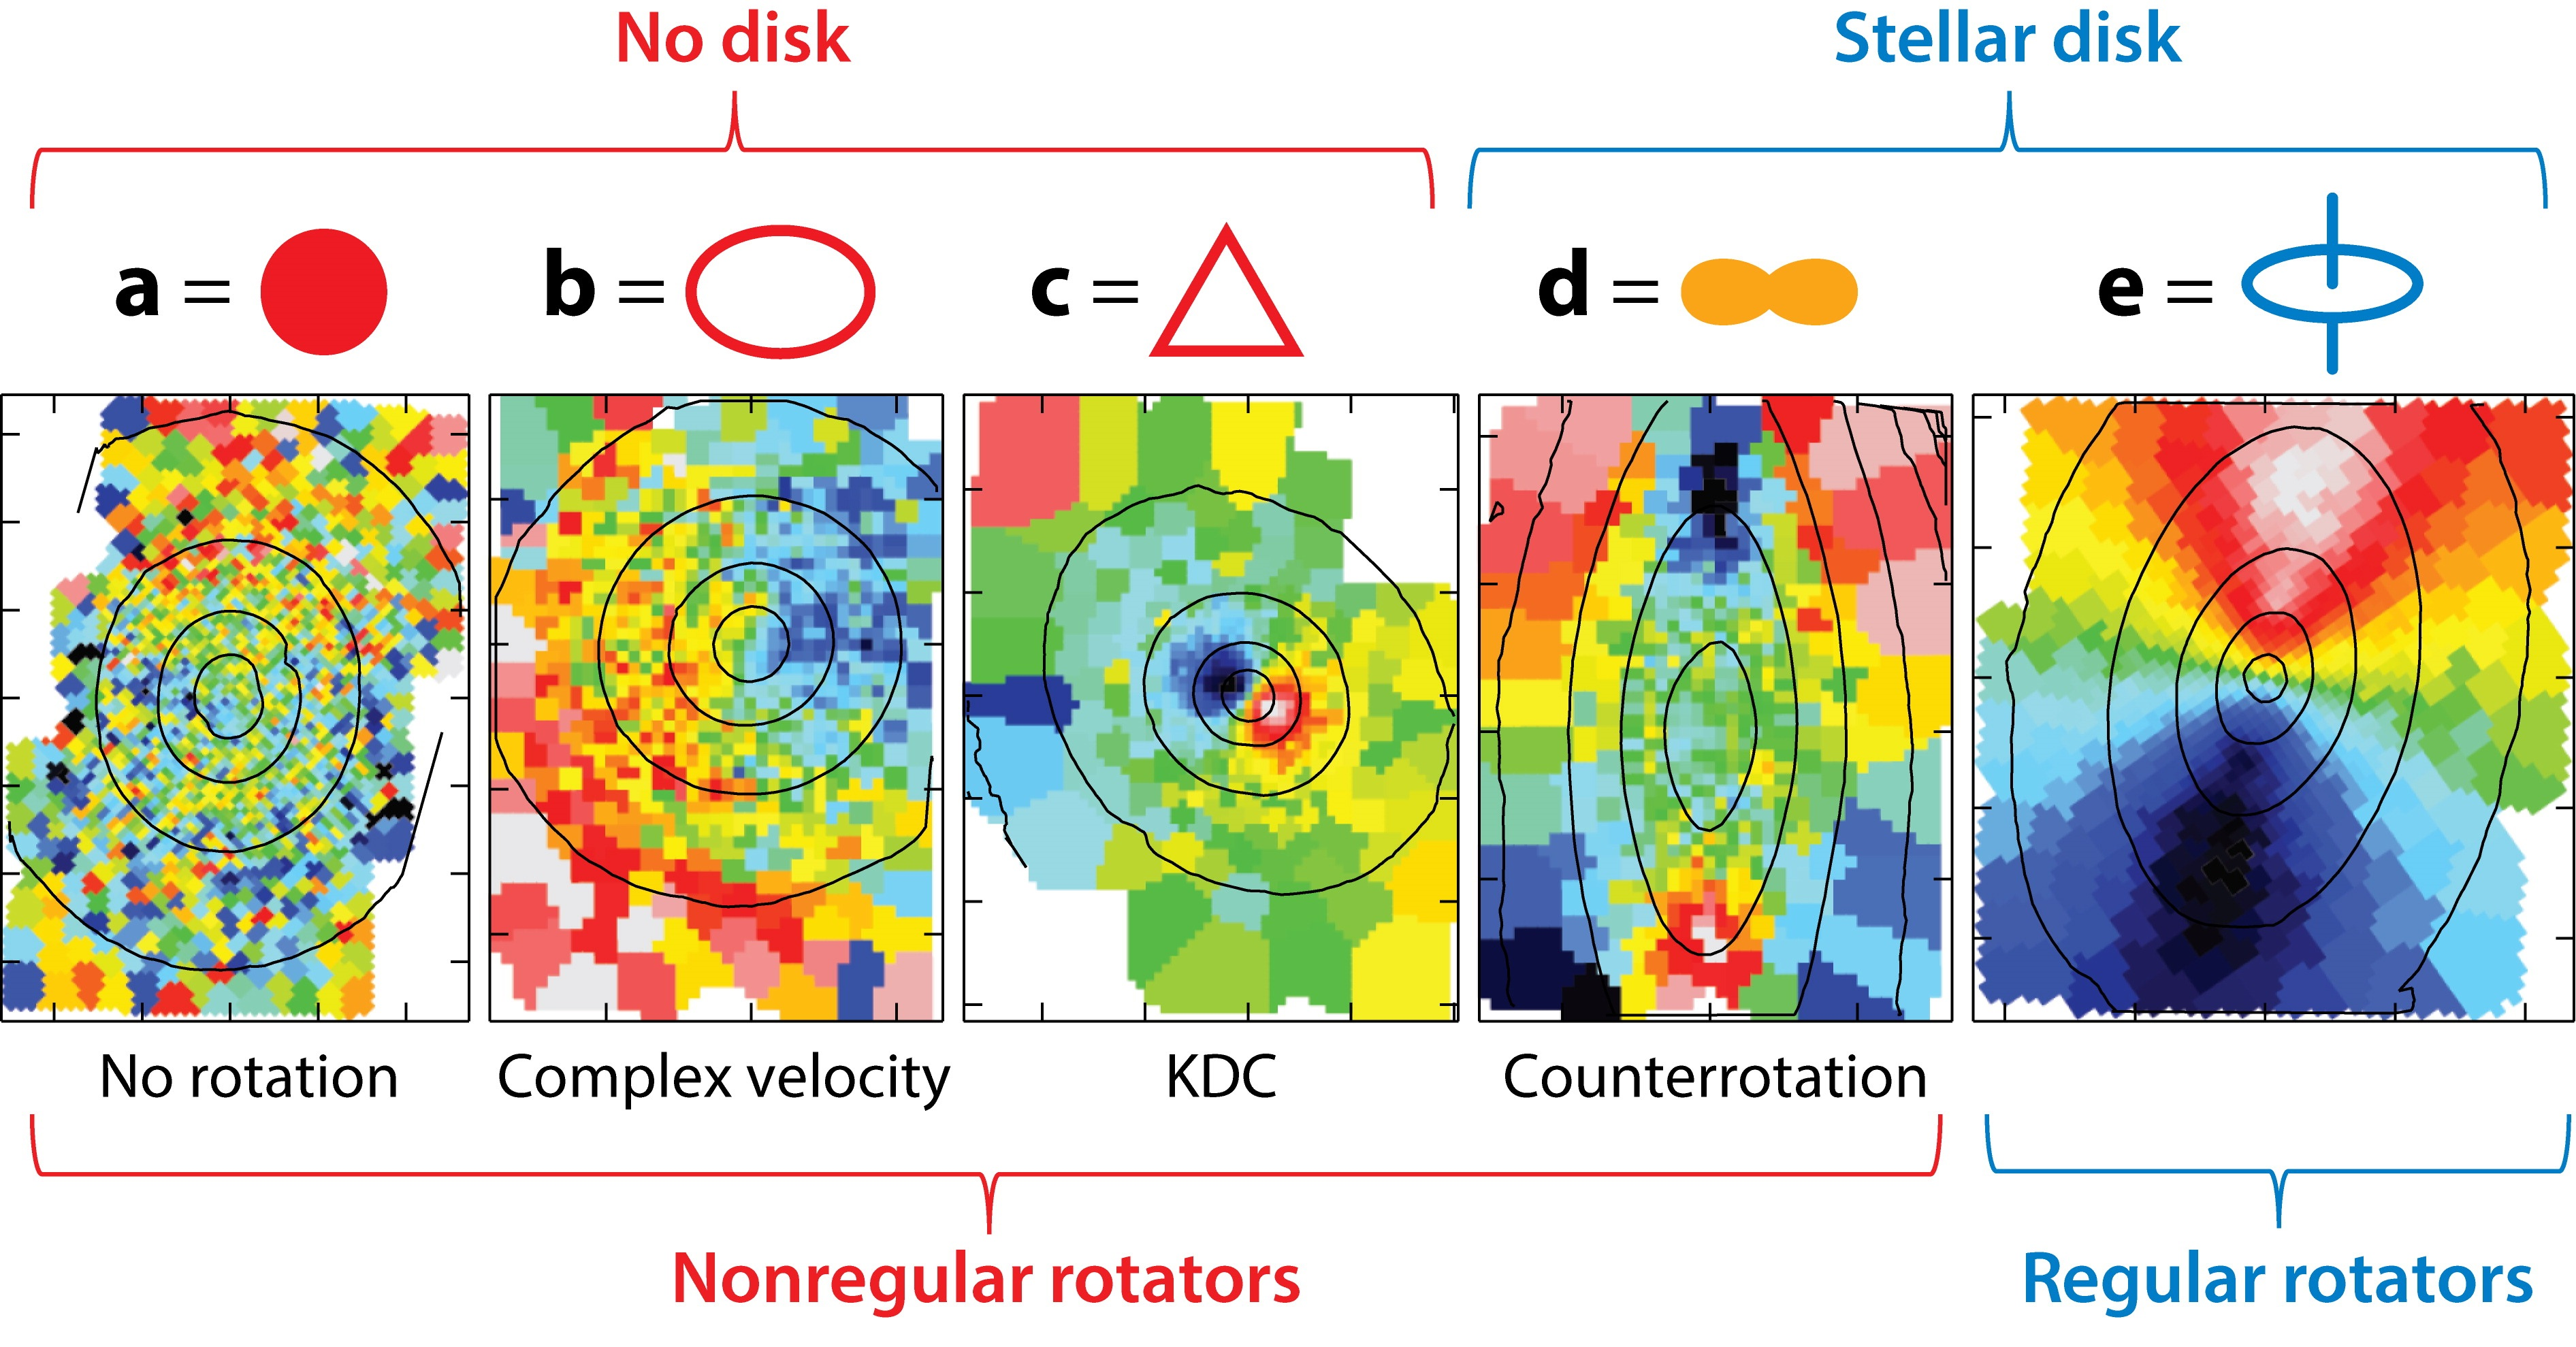
\includegraphics[width=\textwidth]{introduction/substructure.jpeg}
		\caption[Examples of kinematic substructure classifications]{Examples of kinematic substructure classifications of Atlas$^\text{3D}$ (see Table \ref{tab:KinGroups}). Figure courtesy of \citet{Cappellari2016}.}
		\label{fig:EgSubstructure}
	\end{figure}

	Reader wanting more details should consult the excellent review of IFS studies of ETGs: \citet{Cappellari2016}. 


\section{Active Galactic Nuclei}
	\label{sec:AGN}
	The three main issues that astronomers studying AGN focus on are:
	\begin{enumerate}
		\item the origin of the ISM accreted onto the black hole;
		\item the process by which the ISM is accreted; and
		\item any process by which the AGN might affect the host galaxy (feedback).
	\end{enumerate}
	As mentioned previously, the final point has been invoked (and indeed seems to be required) in numerous semi-analytic models and numerical simulations to successfully reproduce the known properties of massive galaxies \citep[e.g.][etc.]{DiMatteo2005, Bower2006, Springel2005}. This mostly involves stopping the bulk of the gas from cooling, such that it can no longer collapse to form stars, with the side-effect that it also self-regulates accretion onto the black hole.

	As previously stated, AGN feedback can be broadly separated into two modes: radiative- and jet-dominated. The former is thought to be the powerful engine that initially rapidly shuts off star formation \citep[e.g.][]{Thomas2005, Thomas2010}, either by removing the cold gas from the galaxy entirely, heating it such that it joins the hot X-ray gas often present in massive galaxies \citep[e.g.][]{OSullivan2001}, or rendering it unusable for star formation (such as by stabilising it against collapse; e.g.\ \citealt{Martig2009}). After a single radiative-mode episode, the AGN is thought to subside to become jet dominated, repeatedly reheating the surrounding ISM to counter any cooling that might allow the cold gas reservoir to replenish (and subsequently form stars). 

	This section will first look at the different AGN global parameters that can be measured. After this, the two different feedback modes (radiative and jet) will be explored.

	\subsection{AGN Parameters}
		\label{subsec:AGNparams}

		\subsubsection{Bolometric Luminosity}
			Perhaps the most basic property of any AGN is its total (bolometric) luminosity. Given the non-spherically symmetric nature of the unified model of AGN, estimating the bolometric luminosity can be a non-trivial task, particularly for obscured (Type 2) AGN. 

		\subsubsection{Black Hole Mass}
			While black holes are not exclusive to AGN, the black hole mass is a parameter useful to understand them, and it is required to calculate the Eddington limit (see Section \ref{subsubsec:Eddington}). Thanks to scaling relations, estimating the black hole mass, $M_\text{BH}$, is relatively simple. In this work we use the black hole mass--galaxy stellar velocity dispersion relation ($M_\text{BH}$--$\sigma_\ast$) of \citet{McConnell2013}:
			\begin{align}
				\log\left(\frac{M_\text{BH}}{\mathrm{M_\odot}}\right) = & \, (8.32 \pm 0.05) + (5.64 \pm 0.32) \log\left(\frac{\sigma_\ast}{200 \, \mathrm{km \, s^{-1}}}\right) \, ,\\
				\intertext{where $\sigma_\ast$ is the luminosity-weighted stellar velocity dispersion within one effective radius, defined as} 
				\sigma_\ast^2 \equiv & \, \frac{\int_0^{R_\mathrm{e}} \left[\sigma^2(r) + v^2(r)\right] I(r) \, \mathrm{d}r}{\int_0^{R_\mathrm{e}} I(r) \, \mathrm{d}r} \, ,
			\end{align}
			where $I(r)$, $v(r)$ and $\sigma(r)$ are the stellar surface brightness, mean velocity and velocity dispersion at a projected radius $r$.


		\subsubsection{Eddington Ratio}
			\label{subsubsec:Eddington}
			The Eddington ratio, $L/L_\text{Edd}$, is the ratio of the bolometric luminosity, $L$, to the maximum luminosity the AGN can achieve while remaining in hydrostatic equilibrium (the Eddington limit $L_\text{Edd}$). The Eddington limit for pure ionised hydrogen is
			\begin{align}
				L_\text{Edd} = & \,\frac{4 \pi G m_\mathrm{p} c}{\sigma_\mathrm{T}} M_\text{BH} \, ,
				\label{eq:eddingtonLimit} \\
				\intertext{where $G$ is Newton's gravitational constant, $c$ is the speed of light, $m_\mathrm{p}$ is is the mass of proton and $\sigma_\mathrm{T}$ is the Thomson scattering cross-section for an electron on a proton. This is evaluated to}
				\frac{L_\text{Edd}}{L_\odot} = & \, 3.3 \times 10^4 \, \frac{M_\text{BH}}{\mathrm{M_\odot}} \, .
			\end{align}
			

	\subsection{Radiative Mode}
		\label{subsec:Radiative}
		Radiative mode AGN (also called quasar mode in the literature) are thought to be black holes that are actively growing as matter falls directly on to the event horizon. In this case, the energy expelled as radiation exceeds that expelled by any jet that may be present (most of the energy of a jet is kinetic): radiative mode AGN are typically radiatively efficient, with Eddington ratios of 1-100\%. In order to achieve this level of radiative efficiency the accretion discs must be geometrically thin as thick discs tend to trap radiation, carrying it back inwards with the accreting material. 

		\subsubsection{Fueling}
			\label{subsubsec:RadiativeFueling}
			The theories for the fueling of radiative-mode AGN broadly fall into two categories: external (e.g.\ mergers or strong tidal interactions) and secular driven. \citet{Heckman2014} argue for of the secular processes and suggest that counter claims have incorrectly handled systematics, though they acknowledge the rare cases of completely bulgeless AGN hosting galaxies such as in \citet{Filippenko1993}, \citet{Satyapal2009} and \citet{Simmons2013} do remain a mystery. 

			One of the main methods to identify mergers or strong interactions in AGN is measuring the lopsidedness, parametrised by the dimensionless quantity $A_1^i$, host galaxies. As detailed in \citet{Reichard2008}, $A_1^i$ is the radially averaged amplitude of the $m=1$ azimuthal Fourier mode between $R_\mathrm{50}$ and $R_\mathrm{90}$, the radii in SDSS $i$-band images enclosing 50\% and 90\% of the total light from the galaxy, normalised to the average surface brightness of the galaxy. They show that while there is a trend for more rapidly growing black holes to be hosted by galaxies with higher average lopsidednesses, but when matched by star-formation history, the AGN hosts showed no excess in lopsidedness. They went on to show that lopsidedness is more strongly correlated with central star formation: it has long been known that interactions drive both lopsidedness and starbursts \citep[e.g.][]{Larson1978}. The stronger dependence of accretion rate on to the black hole on star formation than lopsidedness of the host galaxy is demonstrated in Fig.\,\ref{fig:anisotropy}. This uses the strength of the discontinuity at 4000\,\AA, measured with the dimensionless parameter $D_\mathrm{4000}$, as a proxy for stellar age as young stars produce almost no absorption blue-wards of 4000\,\AA. The quantity, $D_\mathrm{4000}$, is defined as the ratio of the average flux density in the 3750--3950\,\AA\ and 4050--4250\,\AA\ bandpasses. Fig.\,\ref{fig:anisotropy} shows the [\ion{O}{iii}] emission line luminosity (normalised by the black hole mass) is better correlated with the age of the central stellar population than with the lopsidedness of the galaxy. \citet{Heckman2014} interpret this result as ``implying that the fueling of the [AGN] is enhanced by the presence of circumnuclear star formation (and its associated cold gas), but this [AGN] fueling process does not depend upon the way in which this central star formation arises."

			\begin{figure}
				\centering
				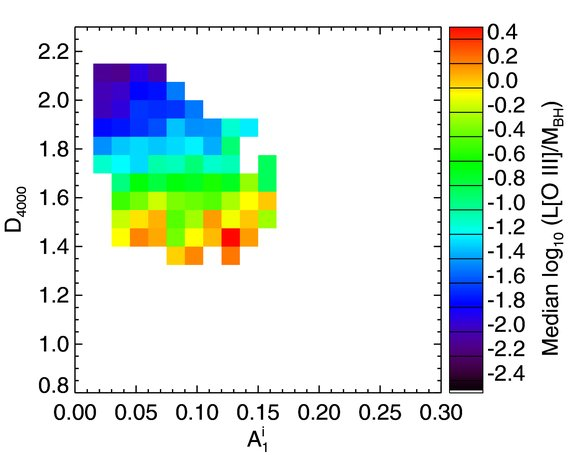
\includegraphics[width=0.6\textwidth]{introduction/age_anisotropy.jpg}
				\caption[The dependence of AGN on age and anisotropies]{AGN strength verses stellar population age and galaxy lopsidedness for SDSS galaxies with redshift $z<0.06$. The AGN strength, quantified by the median luminosity of the [\ion{O}{iii}] emission line normalised by the black hole mass (colour scale) is more strongly dependent on the age of the central stellar population (using $D_\mathrm{4000}$ as a proxy) than on the lopsidedness parameter $A_1^i$. Figure courtesy of \citet{Reichard2009}}
				\label{fig:anisotropy}
			\end{figure}

			Instead, it is thought that secular processes that support inward radial transport of gas are required. These all involve some non-axisymmetric perturbation to the gravitational potential of the galaxy, such as a bar, oval distortion and/or spiral arms \citep[e.g.][]{Kormendy2004, Athanassoula2008, Sellwood2014}. These processes also cause the formation of a so-called pseudobulge, that like a classical bulge is a central region of enhanced surface brightness compared to the extrapolation of the outer (exponential) disc, but unlike a classical bulge is itself disc dominated (i.e.\ dynamically Col.\,) and often contains significant star formation \citep[e.g.][]{Gadotti2009}. \citet{Kormendy2013a} showed that the transition from classical bulges to pseudobulges occurs at a black hole mass of $M_\text{BH} \sim 10^7\,\mathrm{M_\odot}$, corresponding to a bulge stellar velocity dispersion of $\sigma \approx 150 \, \mathrm{km \, s^{-1}}$, which is also where the bulk of local black hole growth is occurring \citep[e.g.][]{Heckman2004, Kauffmann2009}. 

			Finally it is worth noting that bars do not seem to enhance nuclear activity, except that like AGN they are more common in more massive (and redder) galaxies. Once colour and mass are fixed, there is no excess of AGN in strongly-barred galaxies \citep[e.g.][]{Lee2012, Cisternas2013}. This suggests that, while the AGN clearly requires some process to move gas radially inwards, the strength of the AGN is not coupled to the strength of a large-scale bar. 


		\subsubsection{Feedback}
			\label{subsubsec:RadiativeFeedback}
			It is thought radiative mode AGN can also drive powerful interstellar winds, capable of terminating star formation and thus moving a galaxy from the blue cloud to the red sequence. Indeed such strong winds have been observed with velocities in excess of 1000 km s$^{-1}$ \citep{Fischer2010, Feruglio2010, Rupke2011} and \citet{Page2012} showed that (high-level) star formation is present in AGN with X-ray luminosities less than $10^{44} \, \mathrm{erg \, s^{-1}}$, but not above this. Having said that, many radiative-mode AGN actually have circumnuclear star-formation enhancement, presumably due to some of the accreted material being turned into stars \citep[e.g.][]{Santini2012}. 

			The feedback process must also be responsible for maintaining the $M_\text{BH}$--$\sigma_\ast$ relation. If we assume that radiation pressure from an Eddington luminosity AGN sweeps up a gas mass $M_\text{gas} = f M_\text{gal}$ (i.e.\ $f$ is the fraction of the mass of the galaxy, $M_\text{gal}$, that is in the AGN wind), then the force from this radiation pressure, $F_\text{out}$, should match the force due inward gravitational pressure, $F_\text{in}$.
			\begin{align}
				\frac{L_\text{edd}}{c} = F_\mathrm{out} = & \, F_\text{in} = \frac{G M_\text{gal} M_\text{gas}}{r^2} \, , \\
				\intertext{substituting $M_\text{gas} = f M_\text{gal}$, the dynamical mass $M_\text{gal} = \frac{2\sigma_\ast^2 r}{G}$ and Equation \ref{eq:eddingtonLimit}, and rearranging yields}
				M_\text{BH} = & \frac{f \sigma_\ast^4 \sigma_\mathrm{T}}{\pi G^2 m_\mathrm{p}} \, .
				\label{eq:MSigma}
			\end{align}
			This is known as a momentum driven wind \citep[e.g.][]{Fabian1999} and is consistent with some measurements of the $M_\text{BH}$--$\sigma_\ast$ relation, such as that of \citet{Gultekin2009}.
			Another theoretical model for the driving of AGN winds is that they are thermally driven \citep{Silk1998}. This predicts a power-law with an index of $\approx 5$ i.e.\ $\frac{\mathrm{d} \log M_\mathrm{BH}}{\mathrm{d}\log \sigma_\ast} \approx 5$ (as opposed to $\approx 4$ in momentum-driven winds as in Eq. \ref{eq:MSigma}), which is more consistent with more recent measurements of the $M_\mathrm{BH}$--$\sigma_\ast$ relation \citep[e.g.][]{McConnell2013}. 
			Whatever the process that couples the AGN to the winds, the general consensus in the literature is that these winds are responsible for removing or destroying much of the cold gas of the host galaxy, effectively shutting off star formation via the starving of the galaxy of fuel. 
		\subsubsection{Radiative-mode Radio Galaxies}
			\label{subsubsec:RadiativeRadio}
			As stated above, the most powerful RGs are radiative-mode AGN. This is in spite of the fact that RGs are markers for jets (and the radio power is directly correlated with the jet strength). This implies that at these energies, the processes that drive the radiation from the accretion discs must also be more sensitive to the environmental conditions than the processes that drive the jets. RGs are more common at high redshifts, $1.5 \lesssim z \lesssim 3$, which is sometimes called the quasar era \citep{Miley2008}. \citet{Gopal-Krishna2001} suggested that the massive radio lobes from these objects may have been responsible for permeating much of the material that led to the peak of star formation at $z \approx 1.5$. Indeed strong outflows, assumed to be driven by the mechanical energy of the jets, are observed at theses epochs \citep[e.g.][]{Nesvadba2008, Maiolino2012}.
			The broad consensus in the literature is that RGs require a major wet merger to form \citep[e.g.][]{Malin1983, Quillen1992, Lim2000}. Our sample of RGs described in Section \ref{sec:Sample} does not contain any of these extreme galaxies.
	\subsection{Jet Mode}
		\label{subsec:Jet}
		In jet-mode (also called radio- or maintenance-mode in the literature) AGN, the dominant form of emitted energy away from the black hole is the kinetic (i.e.\ mechanical) energy of the material that makes up the jet. Jet-mode AGN can be directly observed `feeding back' to their host galaxies, as jets often terminate at shocks (hot spots) that make up the walls of cavities observed in the hot (X-ray) haloes of the host galaxies.

		Jet-mode AGN tend to be radiatively inefficient, with Eddington ratios $<$ 1\%. This implies that the innermost regions of the accretion discs must be geometrically thick, with inflow times much less than the radiative cooling timescales. The resulting inflows are known as advection-dominated accretion flows (ADAF; \citealt{Narayan1994}). Such systems are capable of launching jets. It is possible that there is a thin disc beyond the thick disc (further from the black hole), but it must be truncated by the thick disc \cite[e.g.][]{Abramowicz2002, Sadler2014}. Much of this is very difficult to resolve observationally, as the spatial scale is $< 100$ Schwarzschild radii, and many of the models remain degenerate \citep[e.g.][]{Quataert1999}. 

		\subsubsection{Fueling}
			\label{subsubsec:JetFueling}
			There is still much speculation about the nature of the fuel (and its origin) in jet-mode AGN, though a consensus seems to building in favour of an internal origin. Many people advocate hot gas as being the ultimate original fuel \citep[e.g.][]{Allen2006}. \citet{Hardcastle2007} suggest that it could be directly accreted through Bondi accretion \citep{Bondi1952}, a simple model where gas is accreted in a spherically-symmetric manner directly from the hot phase onto the black hole. Others invoke a cooling mechanism to allow the X-ray gas to condense into molecular (i.e.\ cold) gas before accretion. Yet others point to a higher higher detection rate of dust and molecular gas in RGs compared to the general population \citep[e.g.][]{Lim2000, DeRuiter2002, Leon2003, VerdoesKleijn2005}, suggesting that cold gas from either internal reservoirs or externally-accreted may be the fuel. \citet{DeRuiter2002} showed that, when dust is present, its mass is correlated with the radio power and there seems to be a bias towards dust lanes orientated orthogonally to radio jets \citep{VerdoesKleijn2005}.

			Beyond this, the source of the energy for powering the jet is still unclear. Energy may be extracted from the black hole via the \citet{Blandford1977} mechanism or variations thereof \citep[e.g.][]{Koide2002}, or from the accretion disc as discussed by \citet{Blandford1982} and others \citep[e.g.][]{Hujeirat2003}. 

		\subsubsection{Feedback}
			\label{subsubsec:JetFeedback}
			It is thought that the duty cycle of a jet is very short; the jet is turned on for very short periods of time before turning off for extended periods. 

			An obvious feedback mode is seen in the haloes of hot X-ray gas around galaxies, where radio jets terminate. The kinetic impacts of the jets create cavities or bubbles in the hot gas (first conceptualised by \citealt{Gull1973}). In cluster environments, these are buoyant and can separate, rising through the intra-cluster medium \citep[e.g.][]{Churazov2000, Churazov2001, McNamara2000}. However, the bubbles are intrinsically anisotropic, while star formation must be suppressed on a global scale. They also exhibit steep abundance gradients, showing that there is little mixing that could disperse energy via convection. Instead, from observations of the very brightest X-ray clusters such as Perseus \citep{Fabian2003, Fabian2006}, Virgo \citep{Forman2007}, Centaurus \citep{Sanders2008}, Abell 2052 \citep{Blanton2011} and simulations \citep[e.g.][]{Ruszkowski2004, Sijacki2006}, it appears that sound waves in the ISM are generated by the repetitive blowing of bubbles. The energy of the waves is likely sufficient to offset that lost by the gas via normal cooling mechanisms \citep{Fabian2003}. The low amplitude of these waves means that they are not detectable in all but the closest clusters (more distant clusters would require in excess of 10 days of continuous \textit{Chandra} observations; \citealt{Graham2008}).

			Even when the jets are turned off or only very weak, the galaxies may still contain low ionisation nuclear emission-line regions (LINERs). It is worth noting that while the most powerful LINERs are likely to be low-luminosity AGN, many (indeed most SDSS-classified LINERs) are not; they belong to a recently-defined category known as LIERs i.e.\ the emission-line region is not nuclear (LINERs but without the `N'; e.g.\ \citealt{Sarzi2005, Sarzi2010, Singh2013, Belfiore2016a}). Such emission is mostly attributed to ionisation from radiation from post-asymptotic giant branch (pAGB) stars. \citet{Capetti2011} suggested using an equivalent width of the [\ion{O}{iii}] emission line of $EW_\text{[\ion{O}{iii}]} = 1$\,\AA\ as a threshold for LIERs; galaxies with greater equivalent widths are likely low-luminosity AGN.

		\subsubsection{Jet-mode Radio Galaxies}
			\label{subsubsec:JetRadio}
			As stated above, most radio emission from RGs results from synchrotron emission from the relativistic plasma within the jets, moving around the magnetic fields tangled in the jets. This means that all such RGs can be considered a jet detection (ignoring the very low radio-luminosity galaxies resulting from high levels of circumnuclear star formation). RGs are always jet-mode AGN, except at the highest radio luminosities where the bright radio jets are dominated (in terms of energy output) by the brighter still accretion disc. These are radiative-mode AGN (see Section \ref{subsubsec:RadiativeRadio}).

			All radio-selected AGN are massive, with very old stellar populations and high concentration indices \citep[e.g.][]{Best2005}. \citet{Best2005} also found that the fraction of galaxies with detectable radio emission is related to the galaxies' stellar and black hole masses by power laws with indices of 2.5 and 1.6, respectively.

	Reader wanting more details on the co-evolution of black holes and host galaxies, and the role of AGN, should consult the excellent reviews by \citet{Fabian2012} and \citet{Heckman2014}. 

\section{Southern Sample}
	\label{sec:Sample}

	\begin{table}
		\centering
		\caption{Key sample selection criteria.}
		\label{tab:selection}
		\begin{tabular}{l c}
			\hline
			\hline
			Declination				& $-17\degree < \delta < -40\degree$ \\
			2.7\,GHz flux density 		& $S_\text{2.7GHz} \ge 0.25 \, \text{Jy} $ \\
			$V$-band apparent magnitude 	& $m_V \le 17.0 $ \\
			Redshift 					& $z < 0.03$ \\			
			\hline
			\hline
		\end{tabular}
	\end{table}

	To study RGs in better detail, a sample of 11 galaxies in the southern hemisphere was constructed by \citet{Prandoni2010}. This sample is similar to the B2 sample of northern hemisphere RGs \citep{Prandoni2007}.

	The Parkes 2.7 GHz survey \citep{Ekers1989} was used as a parent sample, as it contains radio sources (down to a flux density limit of 250\,mJy at 2.7\,GHz) with an optical counterpart (with an $V$-band apparent magnitude of $m_V \le 17.0$). Host galaxies with a redshift greater than 0.03 were discarded. The selection criteria are summarised in Table \ref{tab:selection}. It is worth noting that both the radio and optical limits are apparent measurements, and as such this is not a volume-limited sample.

	\begin{table}
		\centering
	\begin{threeparttable}
		\caption{Key sample characteristics of the Southern Sample galaxies.}
		\label{tab:sample}
		\begin{tabular}{l l r r r l}
			\hline
			\hline
			Host galaxy	& Radio source 	& Redshift	& $S_\text{1.4\,GHz}$	& $m_K$ & Dust morphology\\
						& (PKS) 		& 			& (mJy) 			& (mag)	&\\
			\hline 
			ESO 443-G024 & 1258-321 	& 0.01703	& $1387 \pm 45$		& 8.51 & no dust\tnote{a}	\\ 
			IC 1459 	& 2254-367 		& 0.00565 	& $1280 \pm 45$		& 6.81 & dust lane\tnote{b}	\\
			IC 1531 	& 0007-325 		& 0.02553 	& $388 \pm 12$		& 9.55 & --					\\
			IC 4296		& 1333-\leavevmode\phantom{0}33 		& 0.01248 	& $1342 \pm 41$		& 7.50 & edge-on disc\tnote{b} \\
			NGC 612 	& 0131-\leavevmode\phantom{0}36 		& 0.02954 	& $585 \pm 18$		& 9.58 & dust lane\tnote{c}	\\
			NGC 1316 	& 0320-\leavevmode\phantom{0}37 & 0.00591 	& $255 \pm 10$		& 5.59 & dust patches\tnote{b} \\
			NGC 1399 	& 0336-\leavevmode\phantom{0}35 & 0.00472 	& $209 \pm \leavevmode\phantom{0}7$	& 6.31 & no dust\tnote{b}	\\
			NGC 3100 	& 0958-314 		& 0.00879 	& $530 \pm 16$		& 8.08 & dust lane\tnote{d}	\\
			NGC 3557 	& 1107-372 		& 0.01016 	& $484 \pm 16$		& 7.203 & face-on disc\tnote{b}\\
			NGC 7075 	& 2128-388 		& 0.01819 	& $837 \pm 28$		& 9.56 & --					\\
			--			& 0718-\leavevmode\phantom{0}34 		& 0.02897 	& $1119 \pm 41$		& 9.97 & dust patches\tnote{e} \\
			\hline
			\hline
		\end{tabular}
		\begin{tablenotes}
		\footnotesize
		\note Col.\,1: host galaxy name. Col.\,2: radio source name from Parkes Southern Radio Source Catalogue. Col.\,3: redshift. Col.\,4: National Radio Astronomy Observatory (NRAO) Very Large Array (VLA) Sky Survey (NVSS) 1.4 GHz flux density \citep{Condon1998}. Col.\,5: Two Micron All Sky Survey (2MASS) $K$-band apparent magnitude (with errors of $\pm 0.025$ mag; \citealt{Skrutskie2006}). Col.\,6: dust morphologies from (a) \citet{Govoni2000}, (b) \citet{Lauer2005}, (c) \citet{Bettoni2001}, (d) \citet{Sandage1979}, (e) \citet{Colbert2001}. 
		\item We hereafter refer to the last galaxy by its PKS name only.
		\end{tablenotes}
	\end{threeparttable}
	\end{table}

	These criteria lead to a sample of 11 galaxies hereafter referred to as the Southern Sample. The key observed characteristics are summarised in Table \ref{tab:sample}, while the derived characteristics are listed in Table \ref{tab:sampleDerived}. All galaxies have a FR I radio morphology according to the \citet{Fanaroff1974} scheme; the bulk of the radio emission is centrally-concentrated, as opposed to the FR II morphology where the brightest points are at the ends of the radio lobes. 
	
	The sample was initially observed with the Atacama Pathfinder Experiment \citep[APEX; ][]{Gusten2006}, with detections claimed for the \ce{^{12}CO(2-1)} transition for all galaxies. Some galaxies had extremely large line widths (up to a full-width half-maximum of $904 \, \mathrm{km \, s^{-1}}$ for IC 4296), but most showed a flat or double-horn spectrum indicative of ordered rotation \citep{Prandoni2012}.

	\begin{table}
		\centering
	\begin{threeparttable}[b]
		\caption{Derived characteristics of the Southern Sample galaxies.}
		\label{tab:sampleDerived}
		\begin{tabular*}{\textwidth}{@{\extracolsep{\fill}}l l l l}

			\hline
			\hline
			Host galaxy	& $M_K$ & $\log P_\text{1.4\,GHz}$ & Spectral index 	\\
						& (mag)	& ([W Hz$^{-1}$])		& ([Jy][GHz]$^{-1}$) 	\\
			\hline 
			ESO 443-G024 & -25.86 & 24.0 				& $-0.56 \pm 0.08$	\\
			IC 1459 	& -25.27 & 23.0 				& $\leavevmode\phantom{-}0.25 \pm 0.06$\tnote{a} 	\\
			IC 1531 	& -25.70 & 23.9 				& $-0.33 \pm 0.03$ 	\\
			IC 4296		& -26.18 & 25.4 				& $-1.52 \pm 0.27$ 	\\
			NGC 612 	& -26.01 & 25.0 				& $-1.05 \pm 0.24$ 	\\
			NGC 1316 	& -26.44 & 22.4 				& $-4.7\leavevmode\phantom{0} \pm 2.1\leavevmode\phantom{0}$ 	\\
			NGC 1399 	& -25.25 & 22.5 				& $-0.65 \pm 0.66$ 	\\
			NGC 3100 	& -24.85 & 23.0 				& $-0.40 \pm 0.03$ 	\\
			NGC 3557 	& -26.08 & 23.3 				& $-0.72 \pm 0.13$ 	\\
			NGC 7075 	& -24.98 & 23.9 				& $-0.90 \pm 0.06$ 	\\
			PKS 0718-34 & -25.59 & 24.6 				& $-0.63 \pm 0.06$ 	\\
			\hline
			\hline
			% Also need to correct P_1.4 values are I have changed the S_1.4 values to NVSS in tab:sample
		\end{tabular*}
		\begin{tablenotes}
		\footnotesize
		\note Col.\,1: galaxy name. Col.\,2: $K$-band absolute magnitude. Col.\,3: 1.4 GHz radio power. Col.\,4: radio spectral index (from a straight line fitted to the logarithm of all data points below 10 GHz taken from the Photometric Points tool in the Strasbourg astronomical Data Center (CDS) Portal \citealt{Wenger2000}).
		\item [a] IC 1459 shows a turn over in its spectral energy distribution at $\approx 1 \, \text{GHz}$ (see Fig.\,\ref{fig:ic1459radio}) i.e.\ it is a gigahertz-peaked spectrum (GPS) galaxy. This means the spectral index is very sensitive to the frequency range over which is measured.
		\end{tablenotes}
	\end{threeparttable}
	\end{table}

\chapter{Data Reduction and Analysis}
	\label{cha:Data}
This chapter presents our observations of the Southern Sample (as laid out in Section \ref{sec:Sample}) made with the Visible Multi-object Spectrograph (VIMOS; see Section \ref{sec:VIMOS}) on the European Southern Observatory's (ESO's) Very Large Telescope (VLT). The data-reduction pipeline is described in Section \ref{subsec:VIMOSreduction} along with a discussion of the data quality and the artefacts caused by VIMOS data in Section \ref{subsec:VIMOSartefacts}. A brief discussion of alternative data-reduction pipelines for VIMOS data is given in Section \ref{subsec:Other}. Unpublished archival observations made with the VLT's Multi-unit Spectroscopic Explorer (MUSE) are also used in this project and are described in Section \ref{sec:MUSE}, along with a discussion of ESO's data-reduction pipeline in Section \ref{subsec:MUSEreduction}. Finally, in Section \ref{sec:analysis}, we describe our own data-analysis pipelines, that are used to produce the results presented in Chapters \ref{cha:stellar} and \ref{cha:gas}. 

\section[The Visible Multi-object Spectrograph (VIMOS)]{The Visible Multi-object Spectrograph \\(VIMOS)}
	\label{sec:VIMOS}
	\subsection{VIMOS Instrument}
		VIMOS is a fibre-fed, multi-purpose spectrograph mounted on Unit Telescope 3 (UT3) of ESO's VLT in Paranal, Chile \citep{LeFevre2003}. It has a number of configurations: direct imaging, multi-object spectroscopy (MOS) or integral-field spectroscopy (IFS). For our program, VIMOS was used in IFS mode. 

		The integral-field unit (IFU) has a field of view of $40 \times 40$ spatial pixels (spaxels) with a focal elongator at the entrance to the IFU offering choice of spatial sampling of $0 \farcs67$ or $0 \farcs33$ per spaxel. There are 6 available grisms with varying wavelength ranges and spectral resolutions: low- and high-resolution (LR or HR) red; HR orange; and LR, medium resolution (MR) and HR blue. The observations presented in the following section were obtained using the new (as of March 2012 with our observations obtained in April--November 2012; see Table \ref{tab:observations}) HR blue grism with a spatial sampling of $0 \farcs67$ per spaxel. 

		\begin{figure}
			\centering
			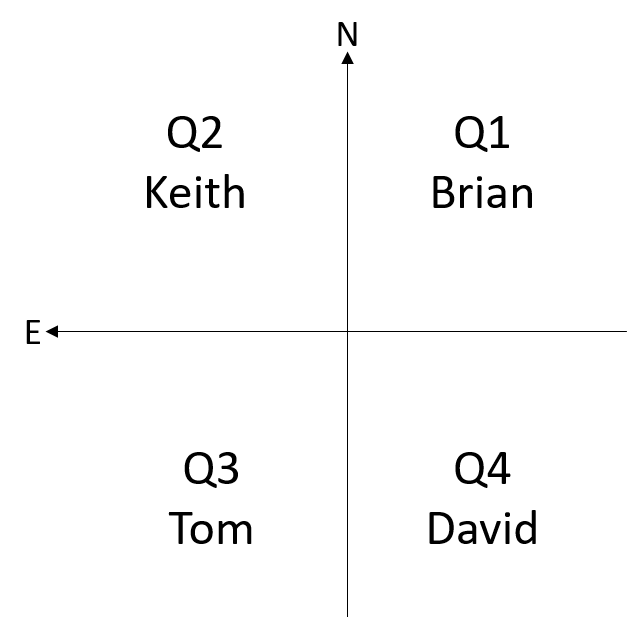
\includegraphics[width=0.4\textwidth]{chapter2/quadrants.png}
			\caption[Schematic of the VIMOS quadrants]{A Schematic of the VIMOS quadrants.}
			\label{fig:quadrants}
		\end{figure}

		The field of view of VIMOS is split into 4 quadrants (cheerfully named in the Flexible Image Transport System, FITS, headers, Brian, Keith, Tom and David). A schematic of the layout is shown in Fig.\,\ref{fig:quadrants}. The quadrants are operated in parallel as independent detectors and it is not possible to use different grisms with different quadrants. The IFU fibres are arranged in a row parallel to and above the short sides of the charge-coupling device (CCD) detectors, and the light from each fibre is then dispersed by the grism in the other direction. This gives rise the to row-stack spectra (RSS) format of most fibre-fed IFU devices.

		VIMOS has several well-known though poorly-understood technical issues. These include several low transmission (bad) fibres, strong flexure and large differences in sensitivity across its 4 quadrants. These are partially dealt with using a specialist data-reduction pipeline described in Section \ref{subsec:VIMOSreduction}, with a discussion of the resulting data quality presented in Section \ref{subsec:VIMOSartefacts} (for more details see the instrument manual, Section 2.8 in the version for Observing Period 100\footnote{\url{http://www.eso.org/sci/facilities/paranal/instruments/vimos/doc.html}}).

	\subsection{VIMOS Observations}
		As stated above, observations for our project were obtained using the VIMOS IFS mode with a spatial sampling of $0\farcs67$ per spaxel and the HR blue grism, yielding a wavelength range of 3700-5520\,\AA\ with a spectral resolution of 1440 and sampling of 0.71\,\AA\,$\mathrm{pix^{-1}}$. Our program (ID: 089.B-0632A) ran in service mode during ESO's period 89 and 90. Each object was observed with a total integration time of $\approx 100$\,min on-source, equally spread over three observing blocks (OBs). Each OB contained 2 science exposures followed by 3 continuum lamp exposures for flatfielding and finally 1 He-Ne arc lamp exposure for wavelength calibration. In addition, the standard VIMOS calibration programme provided 5 bias exposures per night. The flux calibration was calculated using publicly available observations of the spectro-photometric standard star Feige 110 provided by ESO. A summary of the observations is given in Table \ref{tab:observations}.


		\begin{table}
			\centering
		\begin{threeparttable}
			\caption{A summary of the VIMOS observational logs.}
			\label{tab:observations} 
			\begin{tabular}{c c c c c c c}
			\hline
			\hline
				Galaxy 	& OB & Date & Av. DIMM & I. seeing & F. seeing & Airmass \\
				& & (2012) & (arcsec) & (arcsec) & (arcsec) & (arcsec) \\
			\hline
				\multirow{3}{*}{ESO 443-G24}& 1 & 15 Apr & 0.79 & 0.83 & 0.71 & 1.023 \\
				& 2 & 27 Apr & 2.14 & 2.67 & 1.69 & 1.012 \\
				& 3 & 27 Apr & 2.36 & --\tnote{a} & 2.78 & 1.039 \\
			\hline
				\multirow{3}{*}{IC 1459}& 1 & 21 May & 0.82 & 0.84 & 0.82 & 1.238 \\
				& 2 & 28 May & 1.20 & 1.26 & 1.01 & 1.175 \\
				& 3 & 18 Jun & 1.10 & 1.27 & 1.09 & 1.277 \\
			\hline
				\multirow{3}{*}{IC 1531}& 1 & 18 Jun & 1.12 & 1.45 & 1.07 & 1.292 \\
				& 2 & 18 Jun & 1.21 & 1.29 & 1.38 & 1.137 \\
				& 3 & 16 Jul & 1.05 & 1.03 & 0.98 & 1.149 \\
			\hline
				\multirow{3}{*}{IC 4296}& 1 & 23 Apr & 0.78 & 1.00 & 0.61 & 1.015 \\
				& 2 & 23 Apr & 1.09 & 0.90 & 0.86 & 1.101 \\
				& 3 & 23 Apr & 0.86 & 1.07 & 0.89 & 1.224 \\
			\hline
				\multirow{3}{*}{NGC 612}& 1 & 25 Jun & 0.74 & 0.72 & 0.78 & 1.244 \\
				& 2 & 19 Jul & 1.25 & 1.45 & 1.46 & 1.177 \\
				& 3 & 19 Jul & 1.19 & 1.08 & 1.11 & 1.076 \\
			\hline
				\multirow{3}{*}{NGC 1399}& 1 & 27 Jul & 1.09 & 0.95 & 1.28 & 1.314 \\
				& 2 & 29 Jul & 1.02 & 0.95 & 1.04 & 1.219 \\
				& 3 & 15 Aug & 1.51 & 1.06 & 1.57 & 1.281 \\
			\hline
				\multirow{3}{*}{NGC 3100}& 1 & 15 Apr & 0.76 & 0.76 & 0.82 & 1.017 \\
				& 2 & 15 Apr & 0.79 & 0.75 & 0.82 & 1.066 \\
				& 3 & 25 Apr & 1.22 & 1.16 & 1.20 & 1.010 \\
			\hline
				\multirow{3}{*}{NGC 3557}& 1 & 27 Apr & 0.89 & 1.08 & 0.71 & 1.033 \\
				& 2 & 27 Apr & 1.10 & 0.80 & 0.96 & 1.030 \\
				& 3 & 27 Apr & 1.66 & 1.46 & 1.36 & 1.065 \\
			\hline
				\multirow{3}{*}{NGC 7075}& 1 & 18 May & 1.29 & 1.64 & 1.02 & 1.138 \\
				& 2 & 19 May & 0.91 & 1.18 & 0.66 & 1.200 \\
				& 3 & 21 May & 0.87 & 0.80 & 1.33 & 1.229 \\
			\hline
				\multirow{3}{*}{PKS 718-34}& 1 & 15 Apr & 1.02 & 0.99 & 0.95 & 1.113 \\
				& 2 & 16 Apr & 1.05 & 1.25\tnote{b} & 1.05 & 1.126 \\
				& 3 & 12 Nov & 0.69 & 0.68 & 0.65 & 1.146 \\
			\hline
			\hline
		\end{tabular}
			\begin{tablenotes}
			\footnotesize
			\note Col.\,1: Galaxy name. Col.\,2: Observation block (OB) number. Col.\,3: Date of observation. Col.\,4: Average differential image motion monitor(DIMM) during OB. Col.\,5: Initial seeing. Col\,6: Final seeing. Col\.7: Average airmass during OB.
			\item [a] Failed seeing reading at both start and end of first exposure for ESO 443-G24, OB 3 
			\item [b] Failed seeing reading at start of first exposure for PKS 718-34, OB 2. Seeing from end of exposure quoted instead. 
			\end{tablenotes}
		\end{threeparttable}
		\end{table}

	\subsection{VIMOS Data Reduction}
		\label{subsec:VIMOSreduction}
		The data-reduction pipeline we adopted was produced using \textsc{Py3D}, a suite of programs based on the \textsc{python} versions of those developed for the Calar Alto Legacy Integral Field spectroscopy Area survey \citep[CALIFA;][]{Sanchez2012, Husemann2013} but later updated for VIMOS by \citet{Husemann2014}. \textsc{Py3D} was provided to us by Husemann and is not currently publicly available. It makes use of pixel tables to track each pixel throughout the pipeline, with both spectral and spatial resampling only occurring once. The pipeline attempts to account for many of the known issues with VIMOS, such as bad fibres, strong flexure and contamination from adjacent spectra on the CCD (cross-talk), in addition to standard reduction procedures for IFS data. A full outline of the reduction is given below.

		A median `master' bias is first created from the five daily bias frames and subtracted from each raw frame. Known low-transmission (bad) fibres, identified cosmic rays and offsets accounting for flexure of the instrument due to gravity are all considered when automatically identifying the fibre peak positions on the detector. Each fibre is then traced along the dispersion axis in the flat frames. \citet{Husemann2014} find this process to be robust, except for a few fibres at the very blue end of the spectra ($<4300$\,\AA). 

		Since flexure is dependent on the altitude of the pointing of the telescope and the rotation of the instrument, the science exposures will be affected in a manner slightly different than the flatfield exposures. \textsc{Py3D} accounts for these offsets by tracing the peak of the cross-dispersion profile directly on the science exposures at 5 or 6 locations along the dispersion direction for each spectra. The offsets between these positions and the traced spectra at the relevant wavelengths in the flatfield exposures are then interpolated along the dispersion axis with a second order Legendre polynomial. This procedure corrects for the flexure in the cross-dispersion direction, but flexure also affects the dispersion direction due to differences in the pointing of the telescope between the science and arc lamp exposures. This effect is estimated by measuring the positions of strong sky emission lines, but our HR blue grism data have only one sky line at 5199\,\AA, which in many of our science frames was very dim or not detected. This lack of sky lines had previously been an issue with our initial attempt at data reduction using the publicly available \textsc{p3d} suite of programs\footnote{\url{http://p3d.sourceforge.net/}}. Here the lack of sky lines means that \textsc{p3d} is not able to flux calibrate the quadrants with respect to each other. For this reason (and the lack of flexure correction), we use \textsc{Py3D} instead.

		Another issue taken into account by \textsc{Py3D} is cross-talk, where fibres are so densely packed that light from one fibre contaminates (in the cross-dispersion direction) that of neighbouring fibres. The spectra are extracted assuming a Gaussian profile for each fibre in the cross-dispersion direction, with the Gaussian width fitted for each fibre individually. After this, the spectra are adaptively smoothed to a 3\,\AA\ full-width at half-maximum (FWHM) resolution in the dispersion direction and are resampled to a common wavelength solution.

		Flatfields are used to correct for the different transmission efficiencies of the fibres and the different sensitivities of the CCD pixels. Observations of the spectro-photometric standard star Feige 110, recorded in each of the 4 quadrants, are obtained automatically by ESO and are reduced in the same way as described above. Comparisons of the resulting spectra to a reference spectrum of Feige 110 provided by Husemann (private communication) are then used to flux calibrate each quadrant. For each quadrant in every science frame a mean sky spectrum is built using spectra from the outer regions of the field of view and subtracted.

		The quadrants are then combined into a single file, converted from the RSS format to a standard cube (with dimensions of right ascension, declination and wavelength $\lambda$). Finally, the change of the position of the centre of the galaxy with wavelength (due to differential atmospheric refection, DAR) is measured and corrected for. 

		% created with VIMOS_project/reduction/show_corrections.py
		\begin{figure}
			\centering
			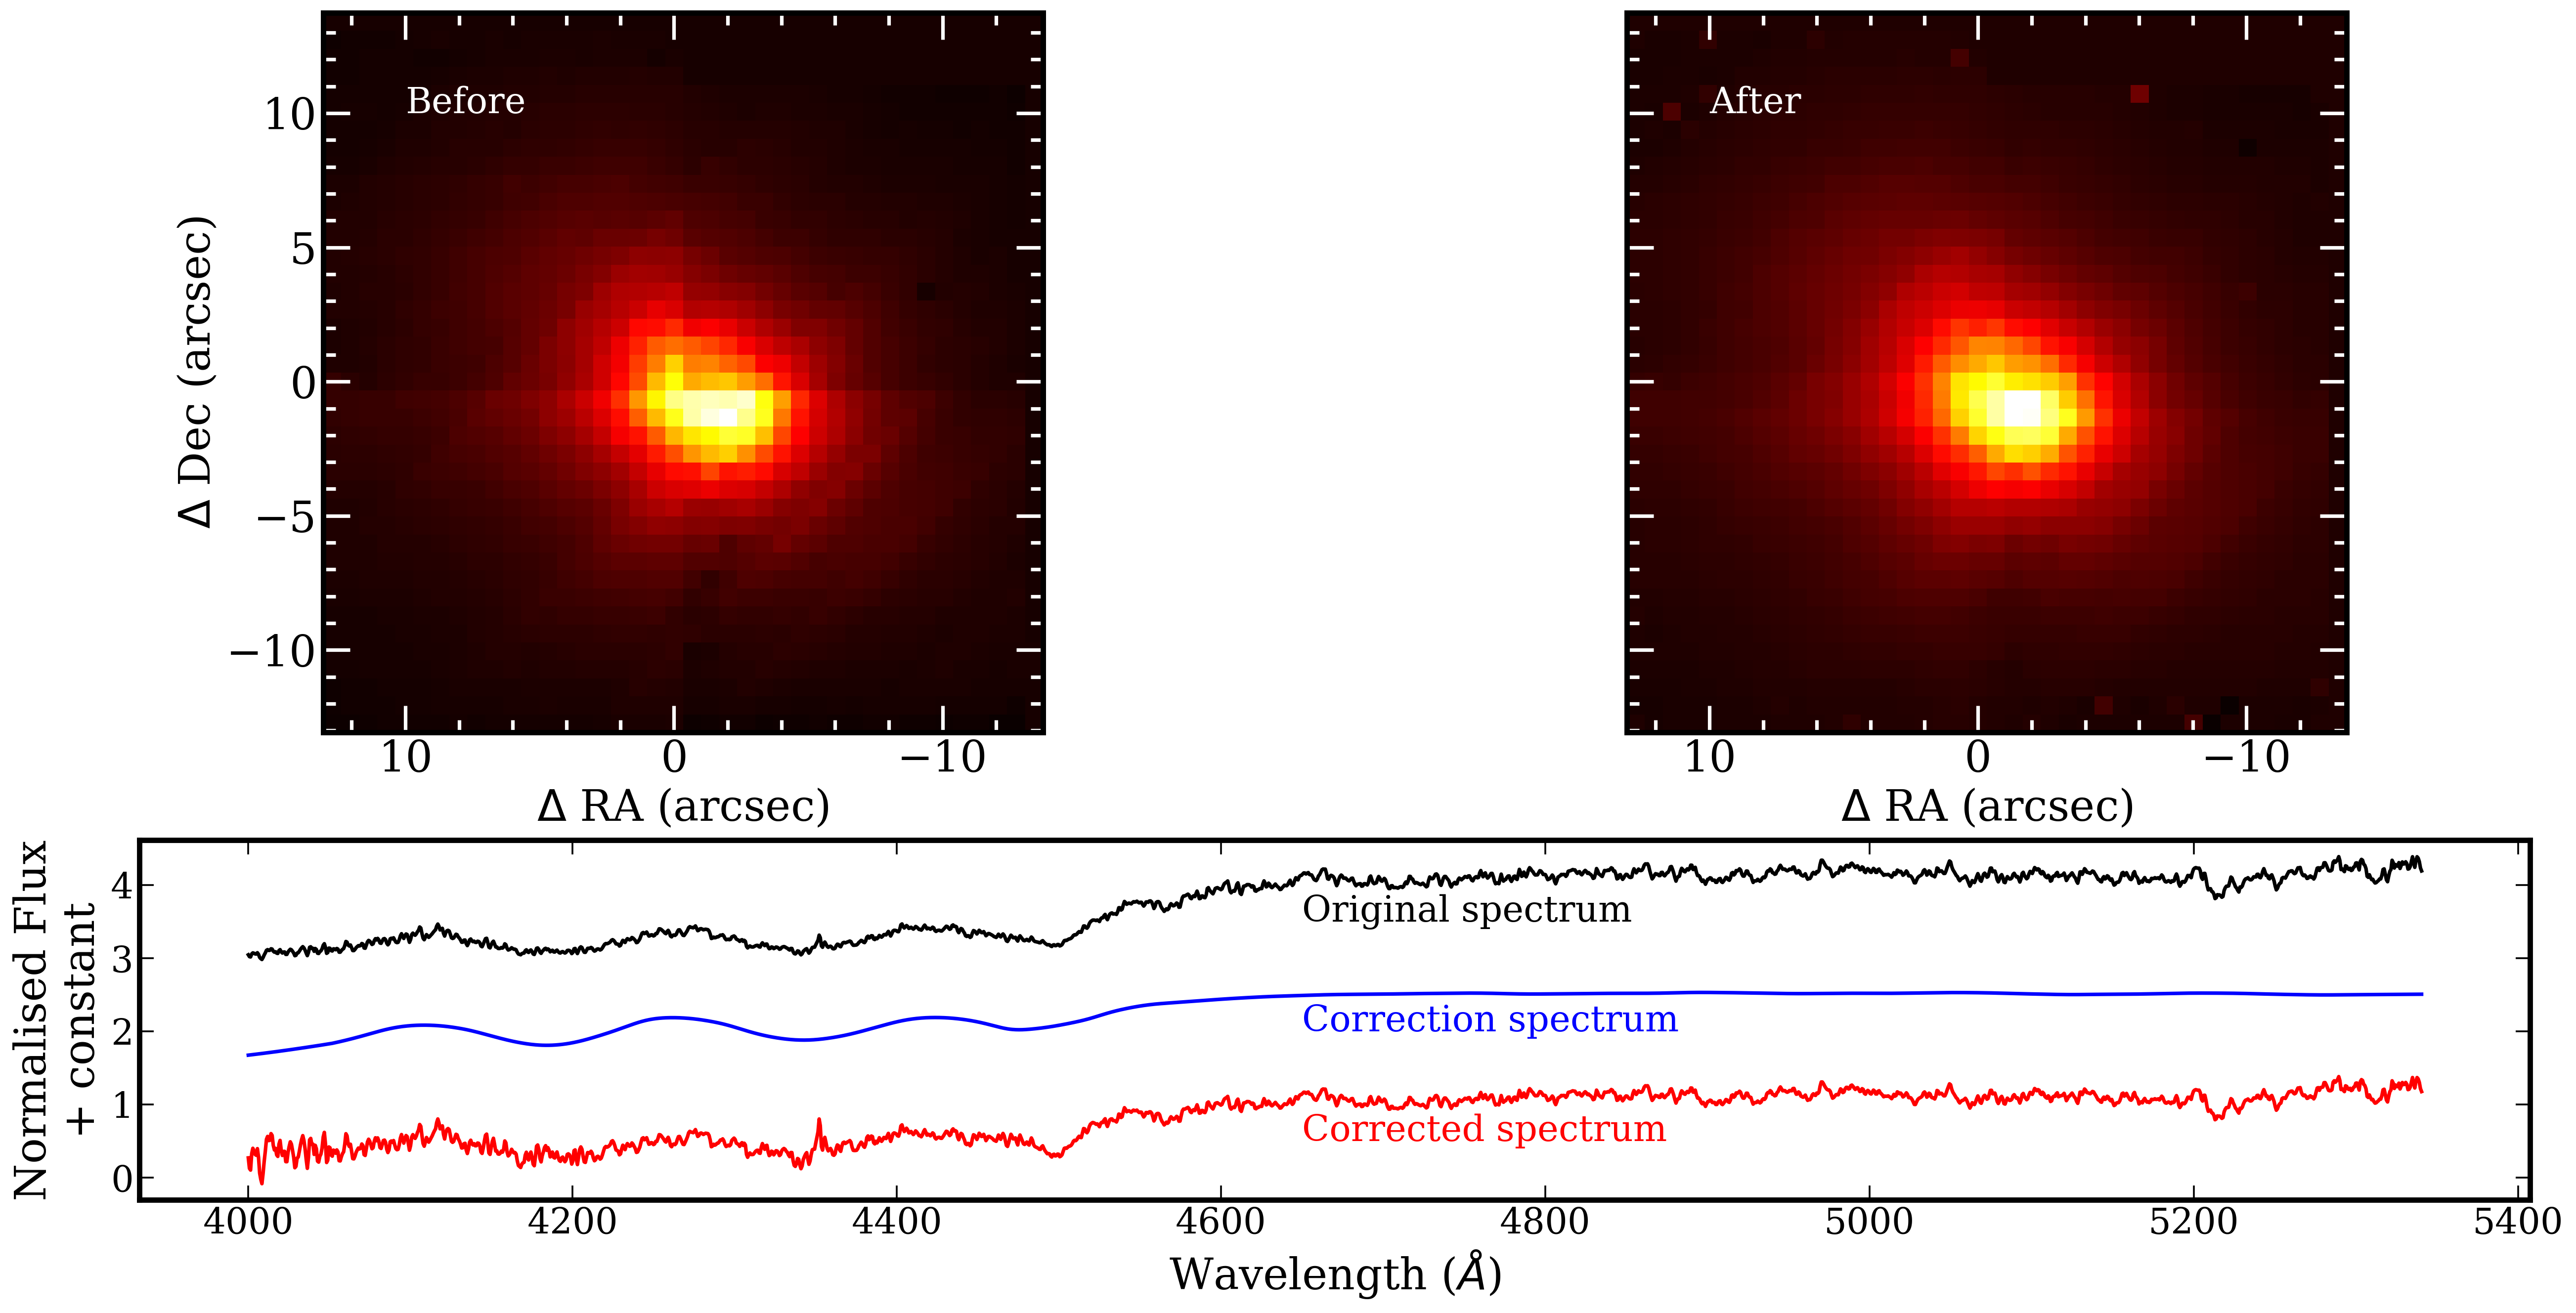
\includegraphics[width=0.99\textwidth]{chapter2/corr_image.png}
			\caption[Ad-hoc correction to the VIMOS datacubes]{Effects of the ad-hoc corrections applied as part of the VIMOS data-reduction pipeline. The top panels show the reconstructed image before (left) and after (right) the ad-hoc corrections are applied to the NGC 3557 datacube. The corrections aim to improve the quadrant-to-quadrant calibration and reduce diagonal intensity stripes. The bottom panel shows an example of the fringe-like pattern correction applied to a single spaxel in NGC 3100.}
			\label{fig:Correction}
		\end{figure}

		Following this, we noted that the cubes were still not properly calibrated. Three main issues remain: the quadrants have different intensities, clearly showing uncorrected throughput differences; diagonal intensity stripes are present in the reconstructed images at all wavelengths; and spectral features are observed \citep{Jullo2008} that are visually similar to fringe patterns caused by interference within the CCD between incident light and light reflected from the interfaces between layers of the CCD materials. Given the thickness of the CCD layers, such fringes should only be observed at $>7000$\,\AA, however they can be seen at all wavelengths, suggesting a different origin. \citet{Lagerholm2012} notes that they appear to be due to altitude angle and hysteresis-dependent reflections occurring within the fibres. We refer to these features hereafter as fringe-like patterns. The first two of these issues are illustrated in the top-left panel of Fig.\,\ref{fig:Correction}. \citet{Lagerholm2012} pointed out that the intensity stripes do not seem to be bound by the quadrants, and concluded that they therefore probably originate from an unknown data-reduction pipeline problem. They however made use of the data-reduction pipeline supplied by ESO\footnote{\url{http://www.eso.org/sci/software/pipelines/vimos/}}, while we use \textsc{Py3D} and also observe the intensity stripes, suggesting that the specific pipeline may not be the cause. 

		These issues were corrected by implementing a \textsc{python} version of the ad-hoc corrections given in \citet{Lagerholm2012}. This involves re-normalizing the quadrants to each other by finding the multiplicative factor for each quadrant which minimizes the differences of the integrated spectra of neighbouring fibres across the edges of neighbouring quadrants (quadrant 2 is held constant). This is followed by the removal of the fringe-like pattern by constructing a correction spectrum by dividing the spectrum of a given fibre by the median spectrum from the eight fibres spatially surrounding it and smoothing over a scale of 150 pixels in the dispersion direction. Each spectrum of the original datacube is then divided by the corresponding correction spectrum (example shown for a single spaxel in NGC 3100 in the bottom panel of Fig.\,\ref{fig:Correction}). The diagonal stripes are not addressed, however the top two panels of Fig.\,\ref{fig:Correction}, which show the reconstructed images (where the datacube is collapsed in the spectral direction) of NGC 3557 before and after these corrections are applied, shows that their impact is significantly lessened by these corrections. This suggests that they may have some connection to the fringe-like patterns. 

		These additional steps mean that the datacubes are not perfectly flux-calibrated, but all the corrections are multiplicative and thus will not effect equivalent width measurements. From comparisons to the MUSE data (see Section \ref{sec:MUSE}), we can then estimate the flux calibration of the resulting datacubes. 

		The variance spectra are propagated throughout the data-reduction pipeline (including these ad-hoc corrections) and are square-rooted at this point, to be used as noise inputs in the following analyses (see Section \ref{sec:analysis}).

	\subsection{VIMOS Data Quality}
		\label{subsec:VIMOSartefacts}
		By comparing the top panels of Fig.\,\ref{fig:Correction}, we can clearly see that while there is an obvious improvement of the calibration between the quadrants, there are still sharp offsets. This often gives rise to diamond-shaped rather than elliptical isophotes. Neighbouring spaxels along the quadrant edges can have fluxes that are different by as much as 20-30\%. Luckily, the worst affected galaxies are IC 4296 and NGC 1399, for which MUSE archival data are available (see Section \ref{sec:MUSE}). 

		Similar offsets are also observed in the spectral direction, with a slight offset of the absolute wavelength calibration between quadrants. This is most clearly seen in the mean velocity maps after the routines described in Section \ref{subsec:StellarFit} are applied. For example the left panel of Fig.\,\ref{fig:egVel} shows the mean stellar velocity map of NGC 1399. The top-right quadrant clearly has a slightly higher velocity than would be expected for a normal rotating galaxy. This corresponds to a shift of the galaxy spectra with respect to the reference wavelength frame (i.e.\ the arcs lamp lines). For comparison, the right panel of Fig.\,\ref{fig:egVel} shows the mean stellar velocity map of the same galaxy from a different instrument, that does not suffer from this problem. Again, the worst affected galaxies are IC 4296 and NGC 1399.

		\begin{figure}
			\centering
			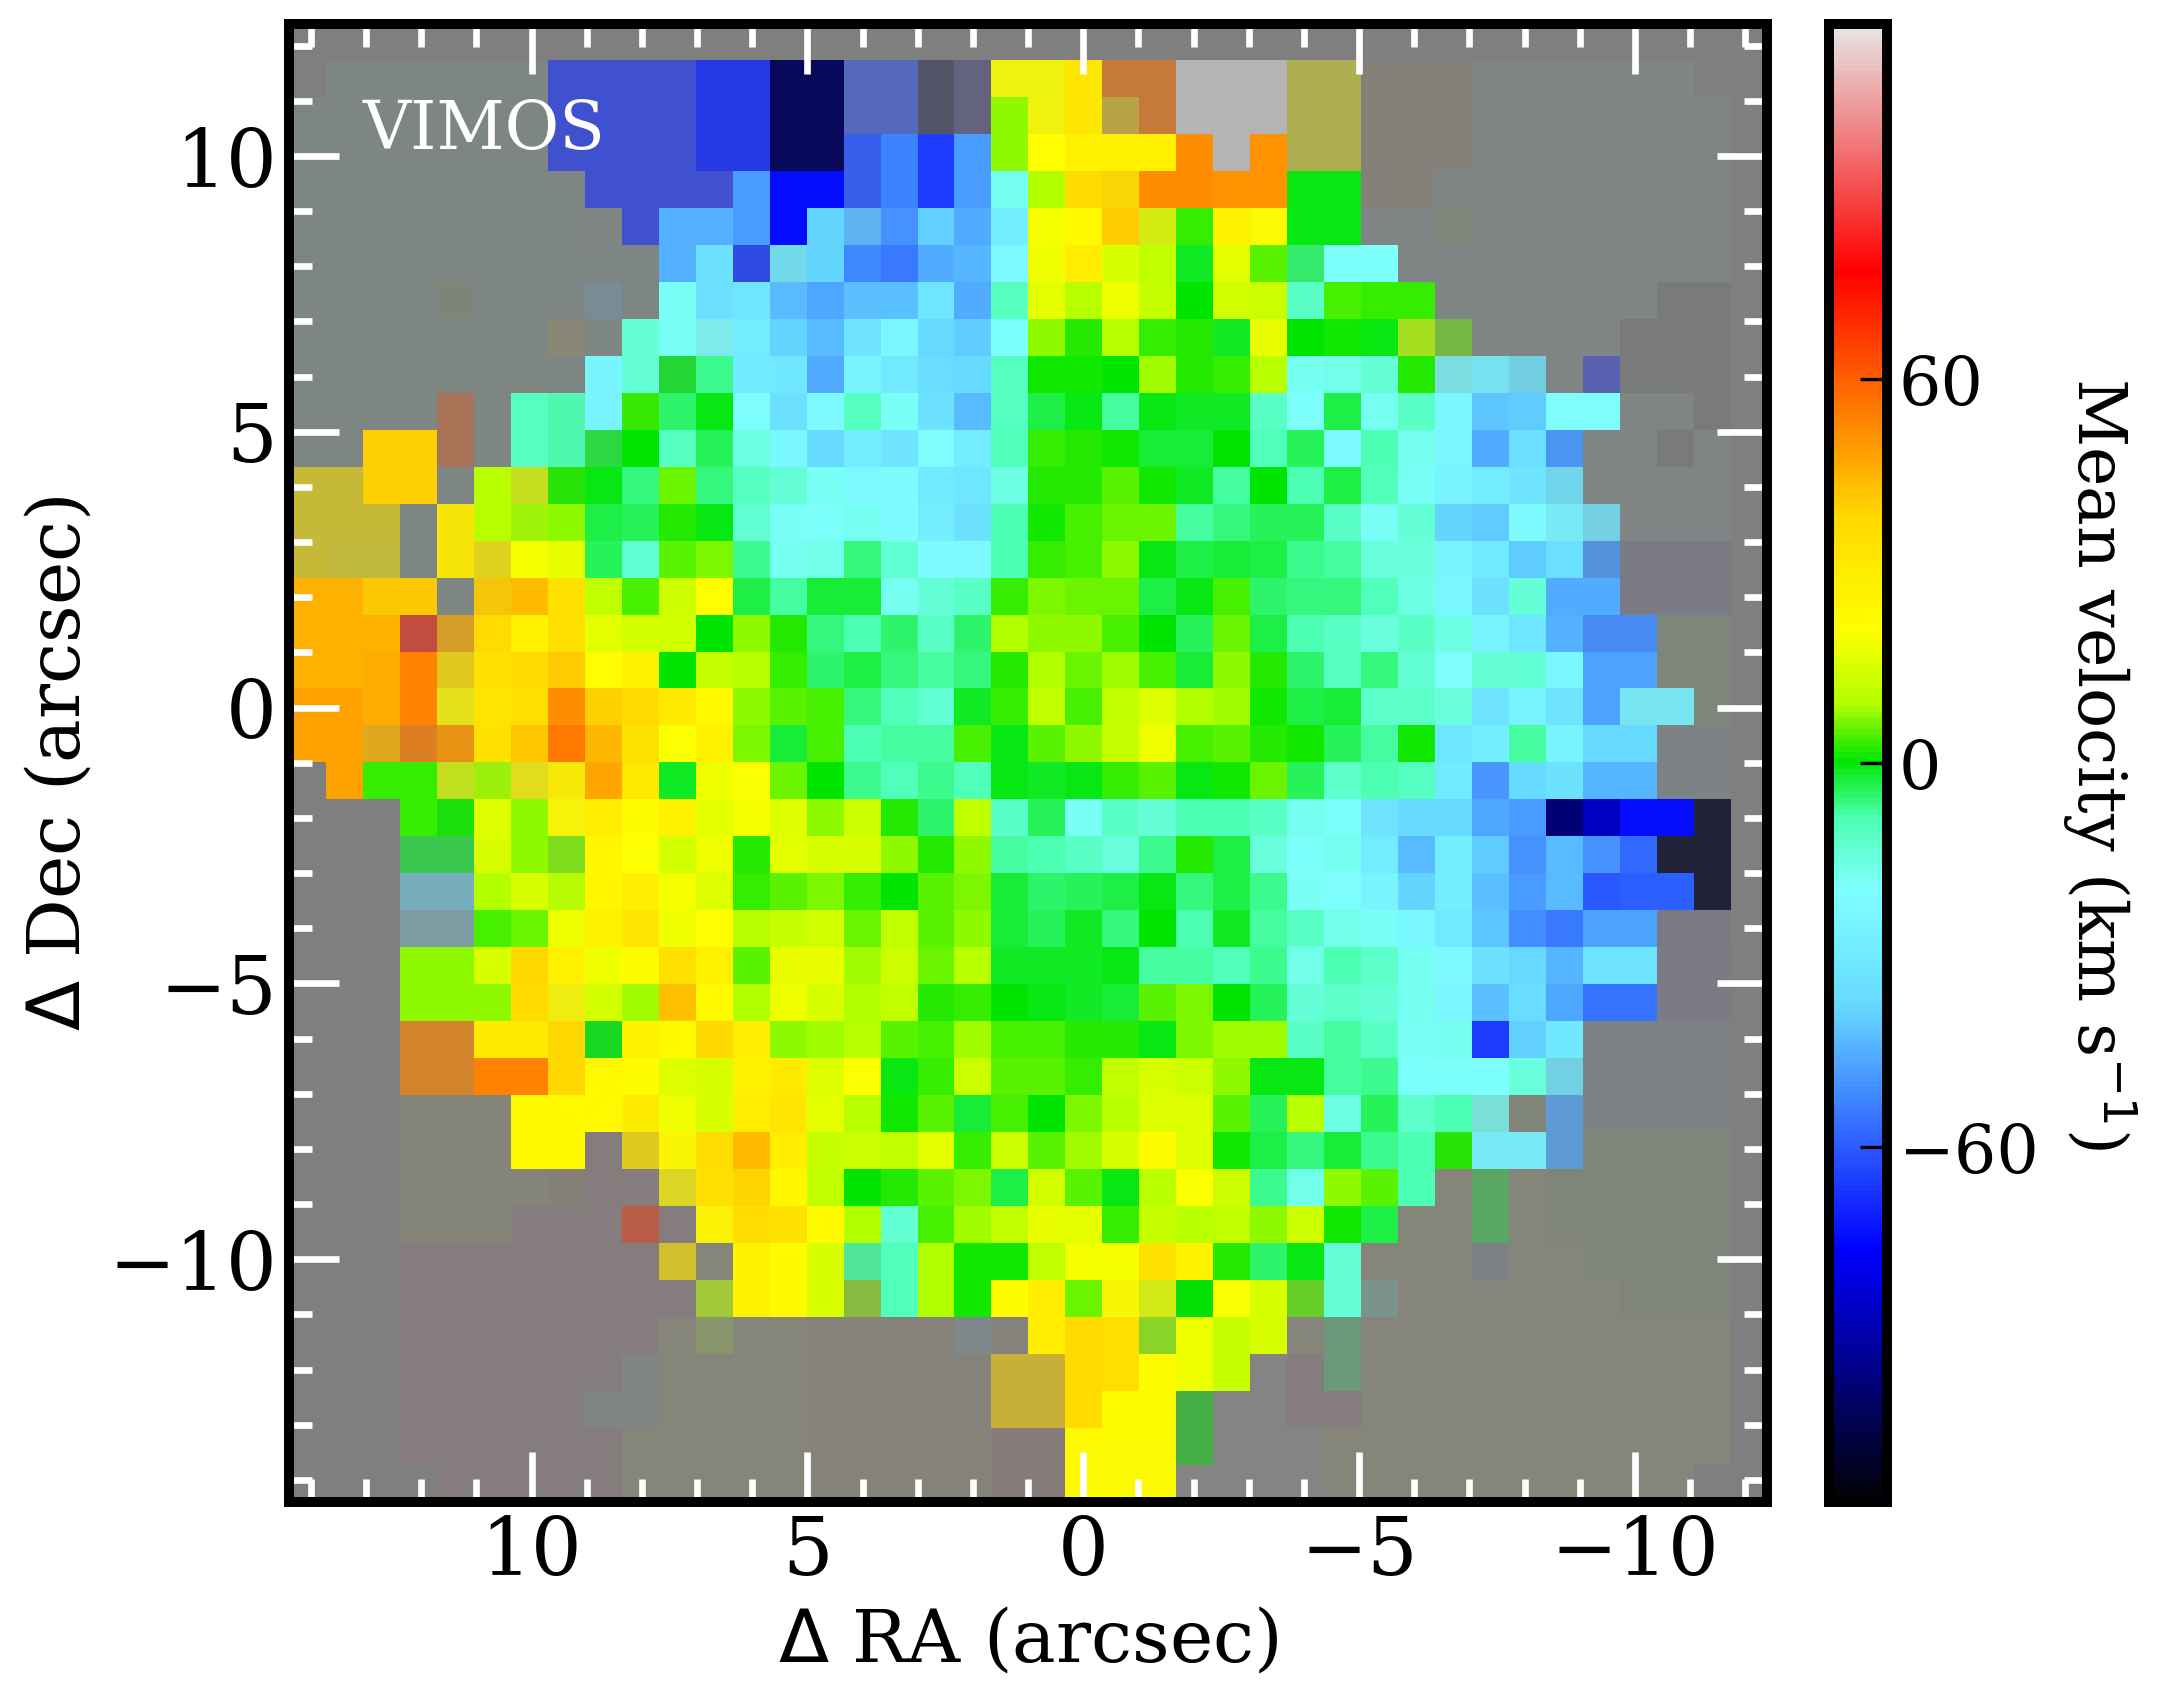
\includegraphics[width=.4\textwidth]{chapter2/VIMOS_NGC1399_vel.png}
			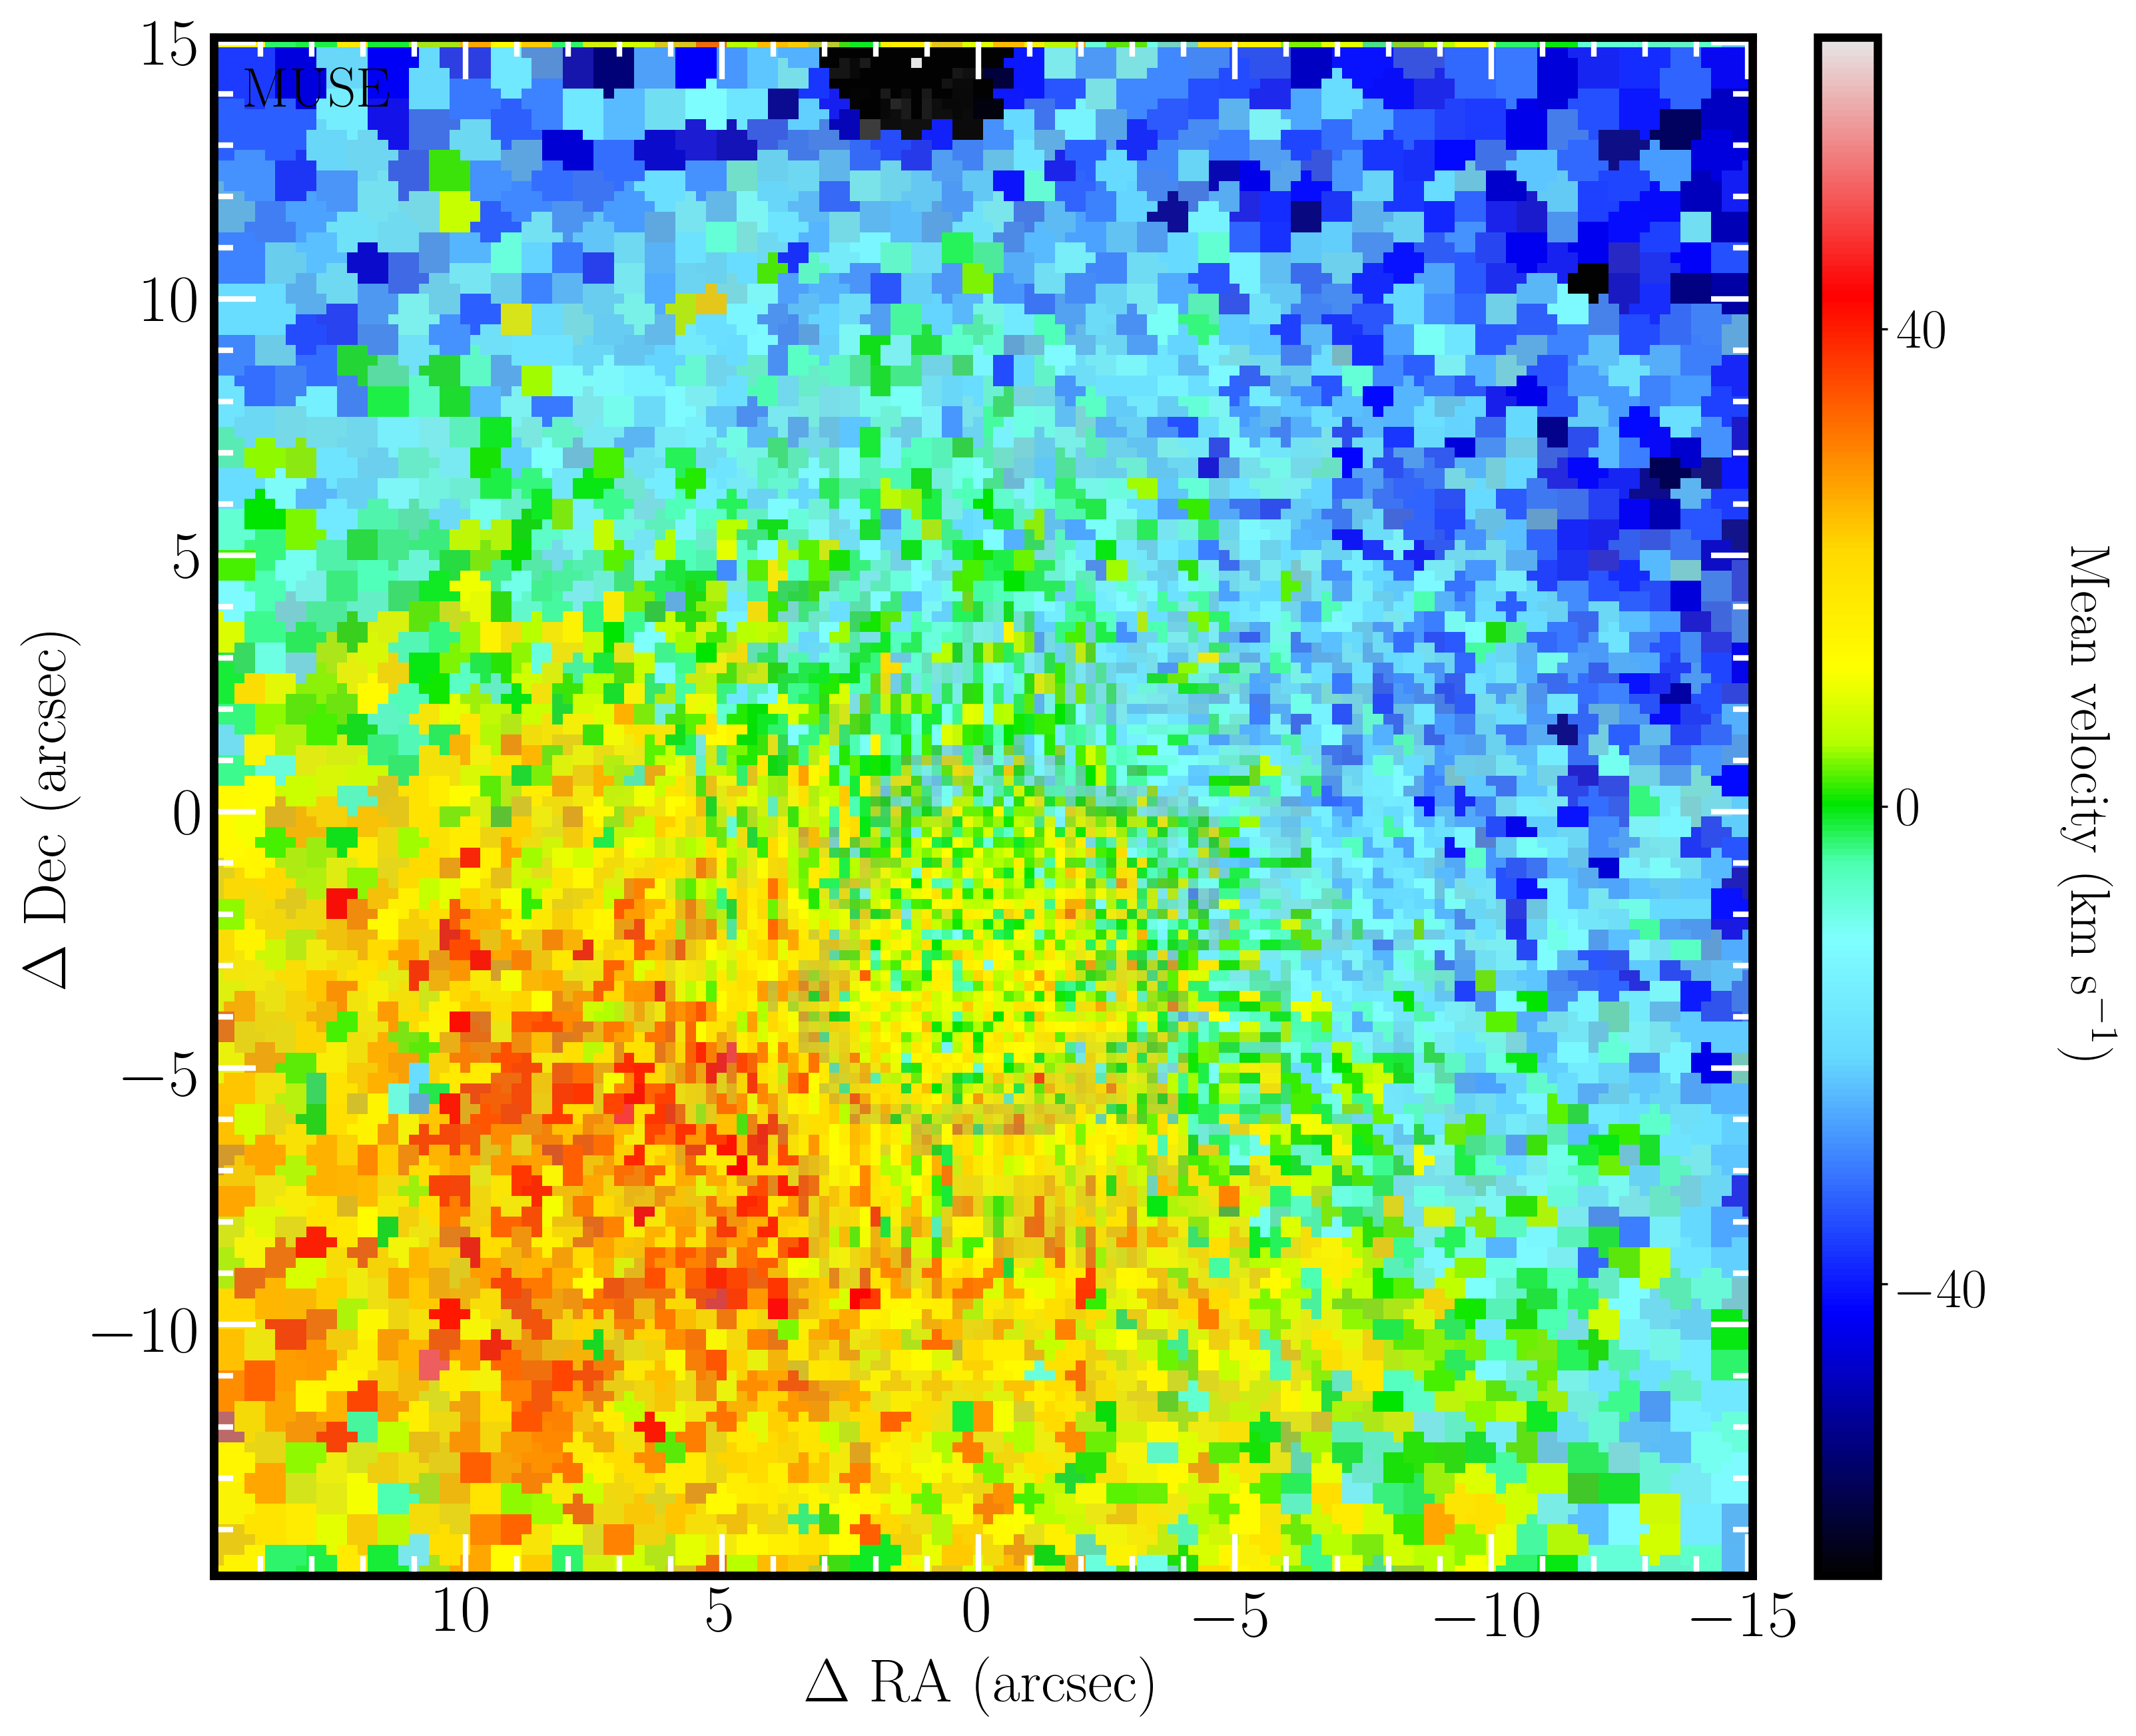
\includegraphics[width=.4\textwidth]{chapter2/MUSE_NGC1399_vel.png}
			\caption[VIMOS data wavelength calibration problems]{Mean stellar velocity maps of NGC 1399, demonstrating the wavelength calibration offsets between the different quadrants of VIMOS. Left panel: VIMOS map. Right panel: MUSE map (see Section \ref{sec:MUSE}).}
			\label{fig:egVel}
		\end{figure}

		\begin{figure}
			\centering
			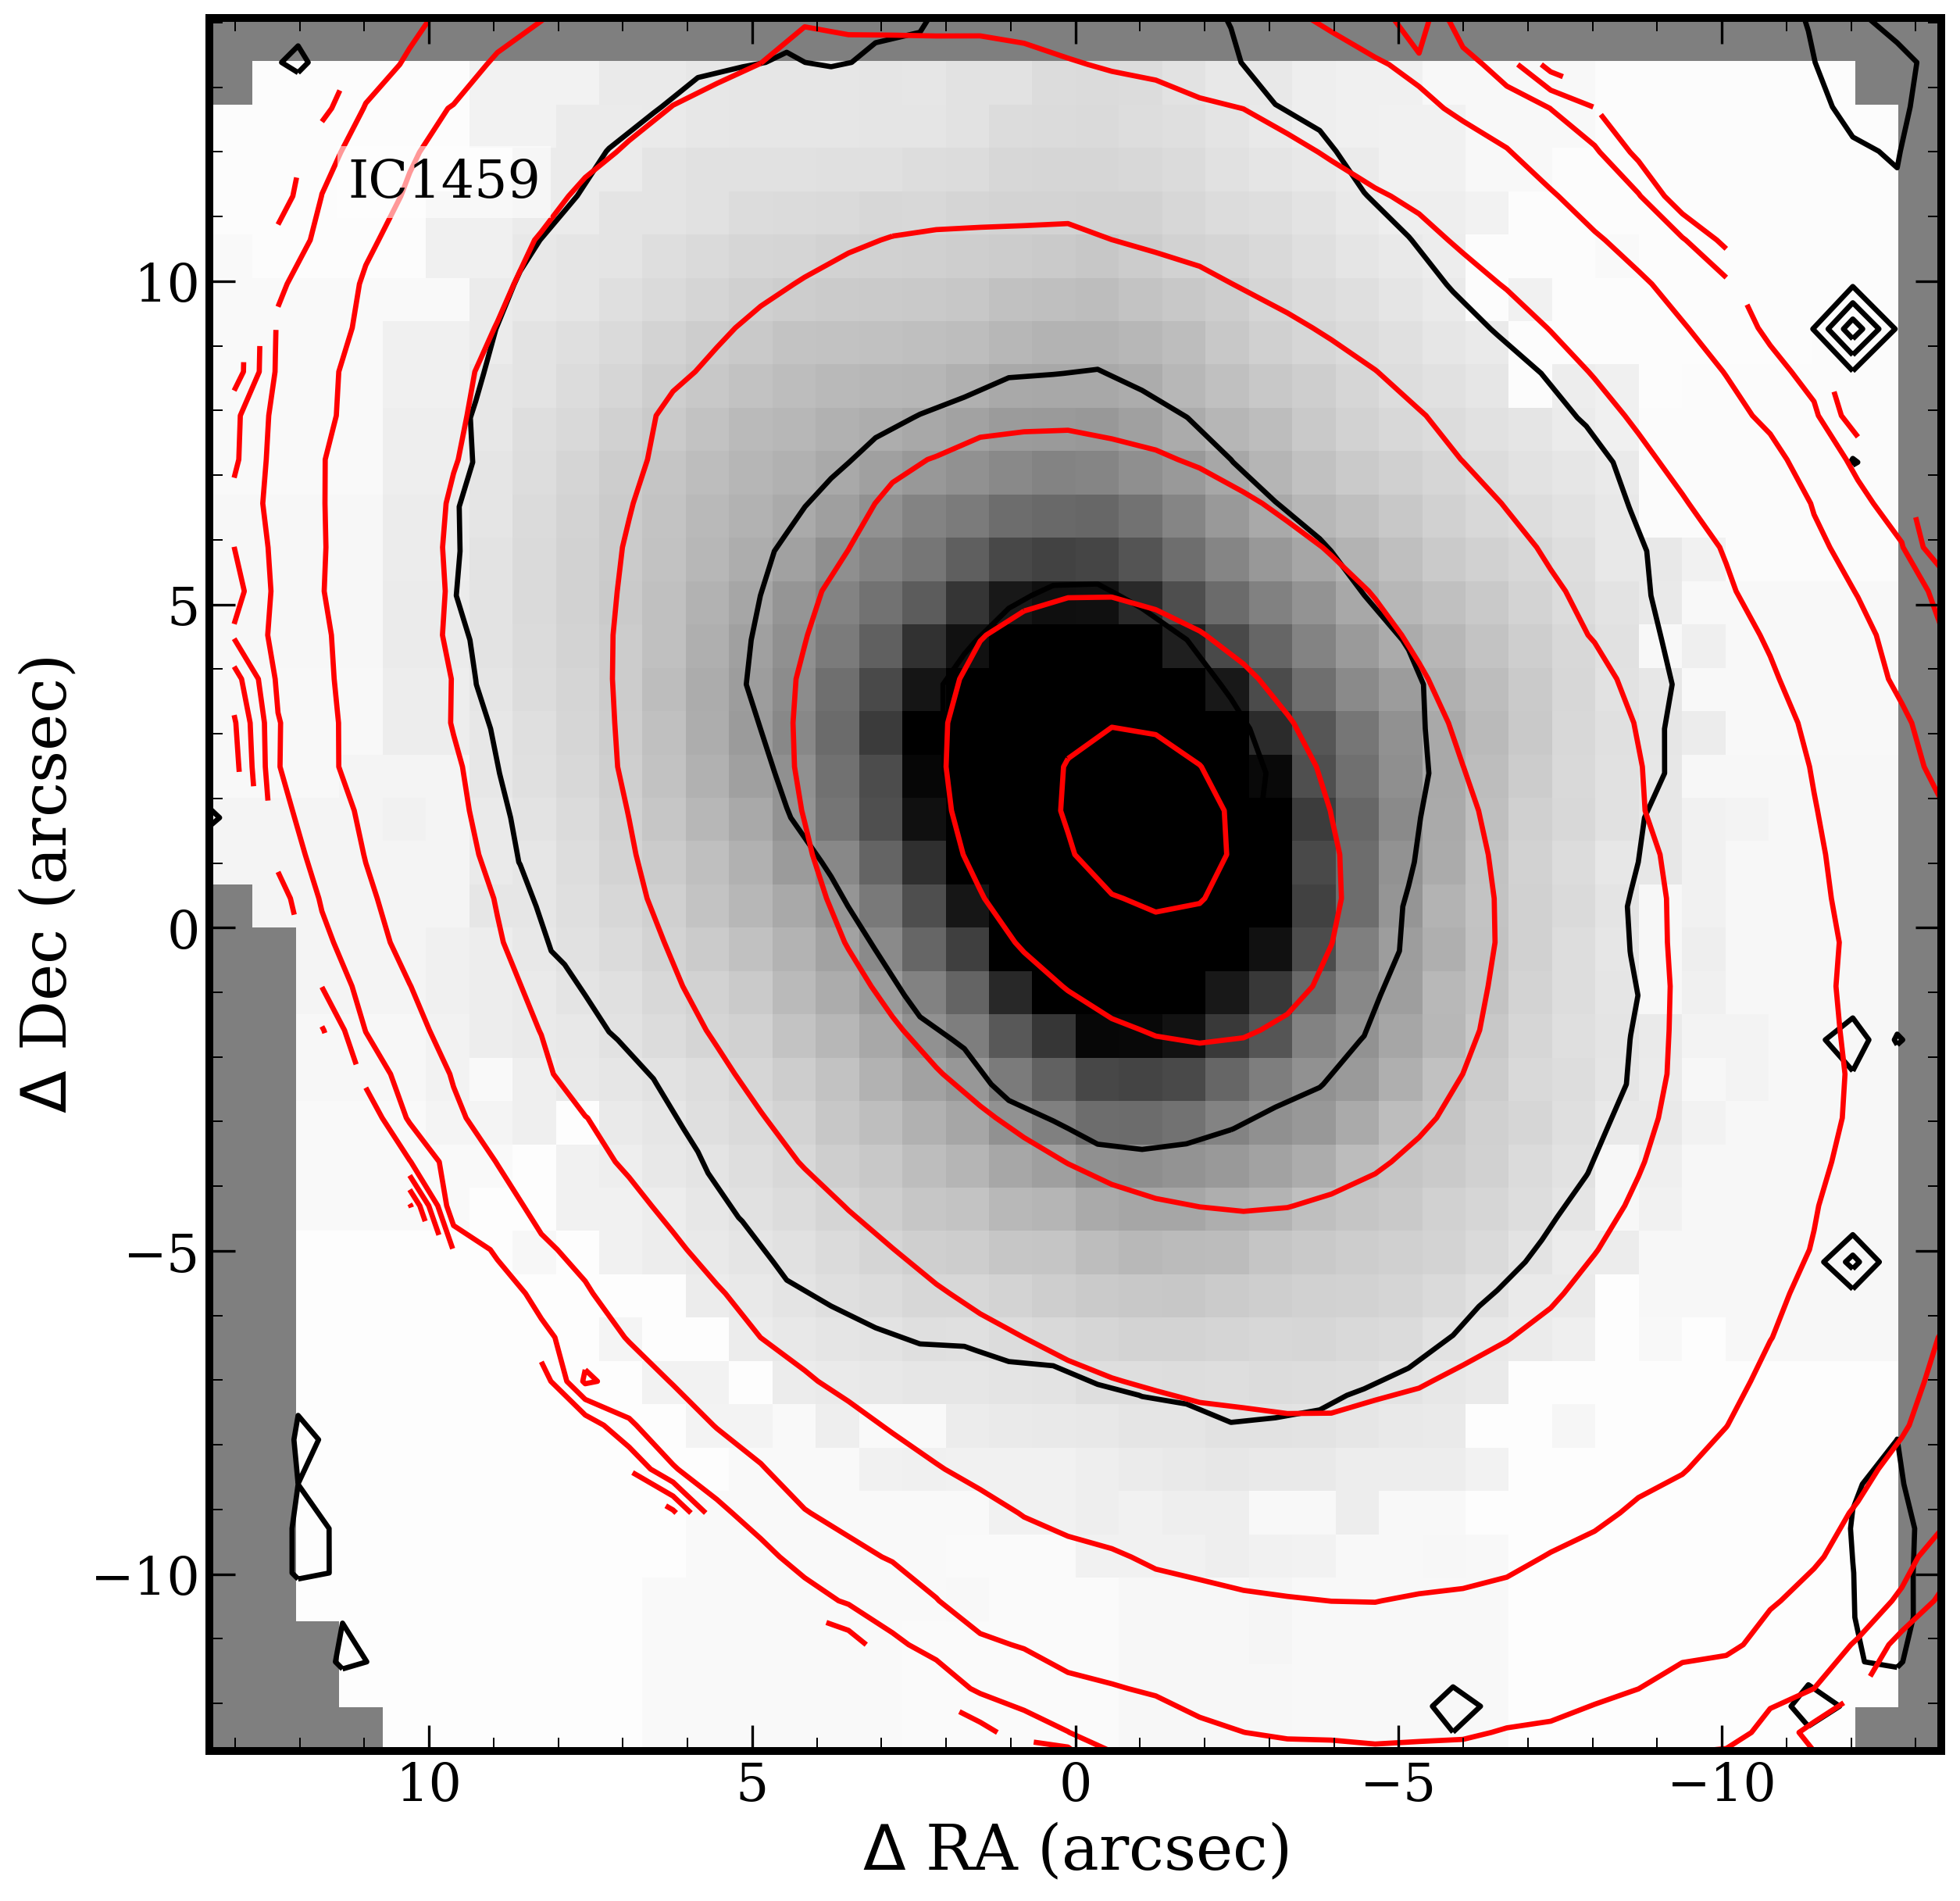
\includegraphics[width=.4\textwidth]{chapter2/hst_vimos_ic1459.png}
			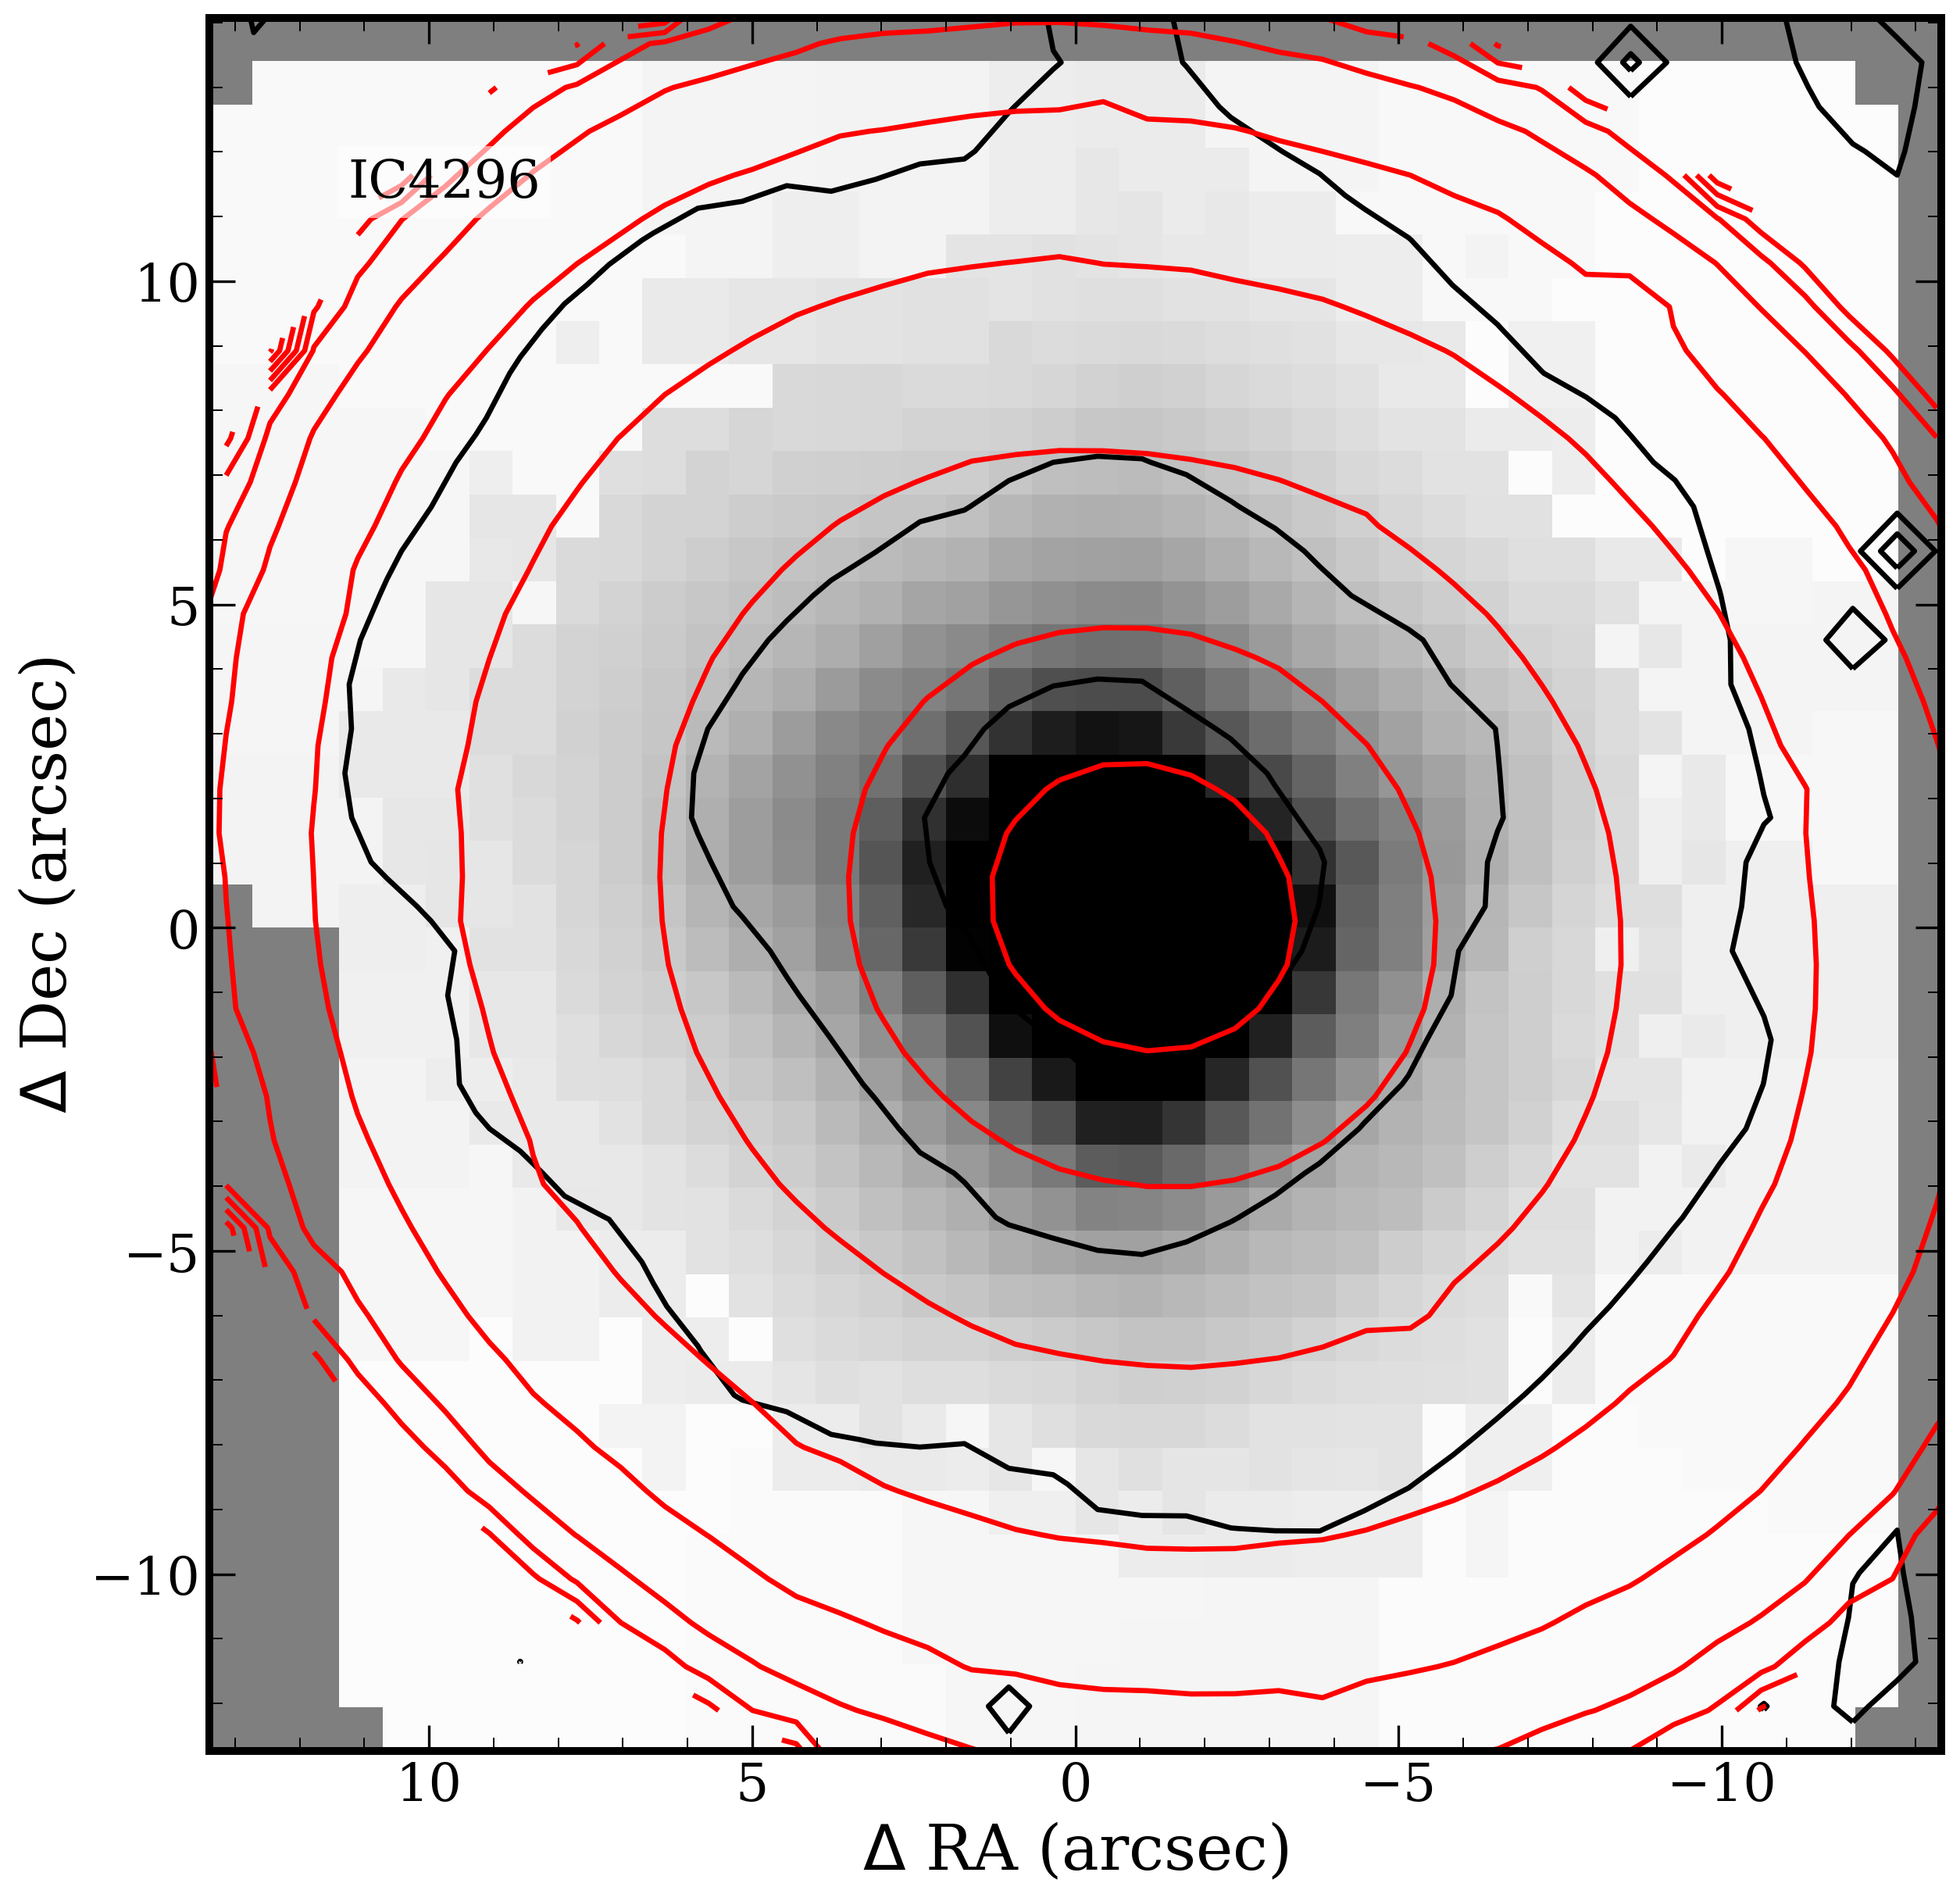
\includegraphics[width=.4\textwidth]{chapter2/hst_vimos_ic4296.png}
			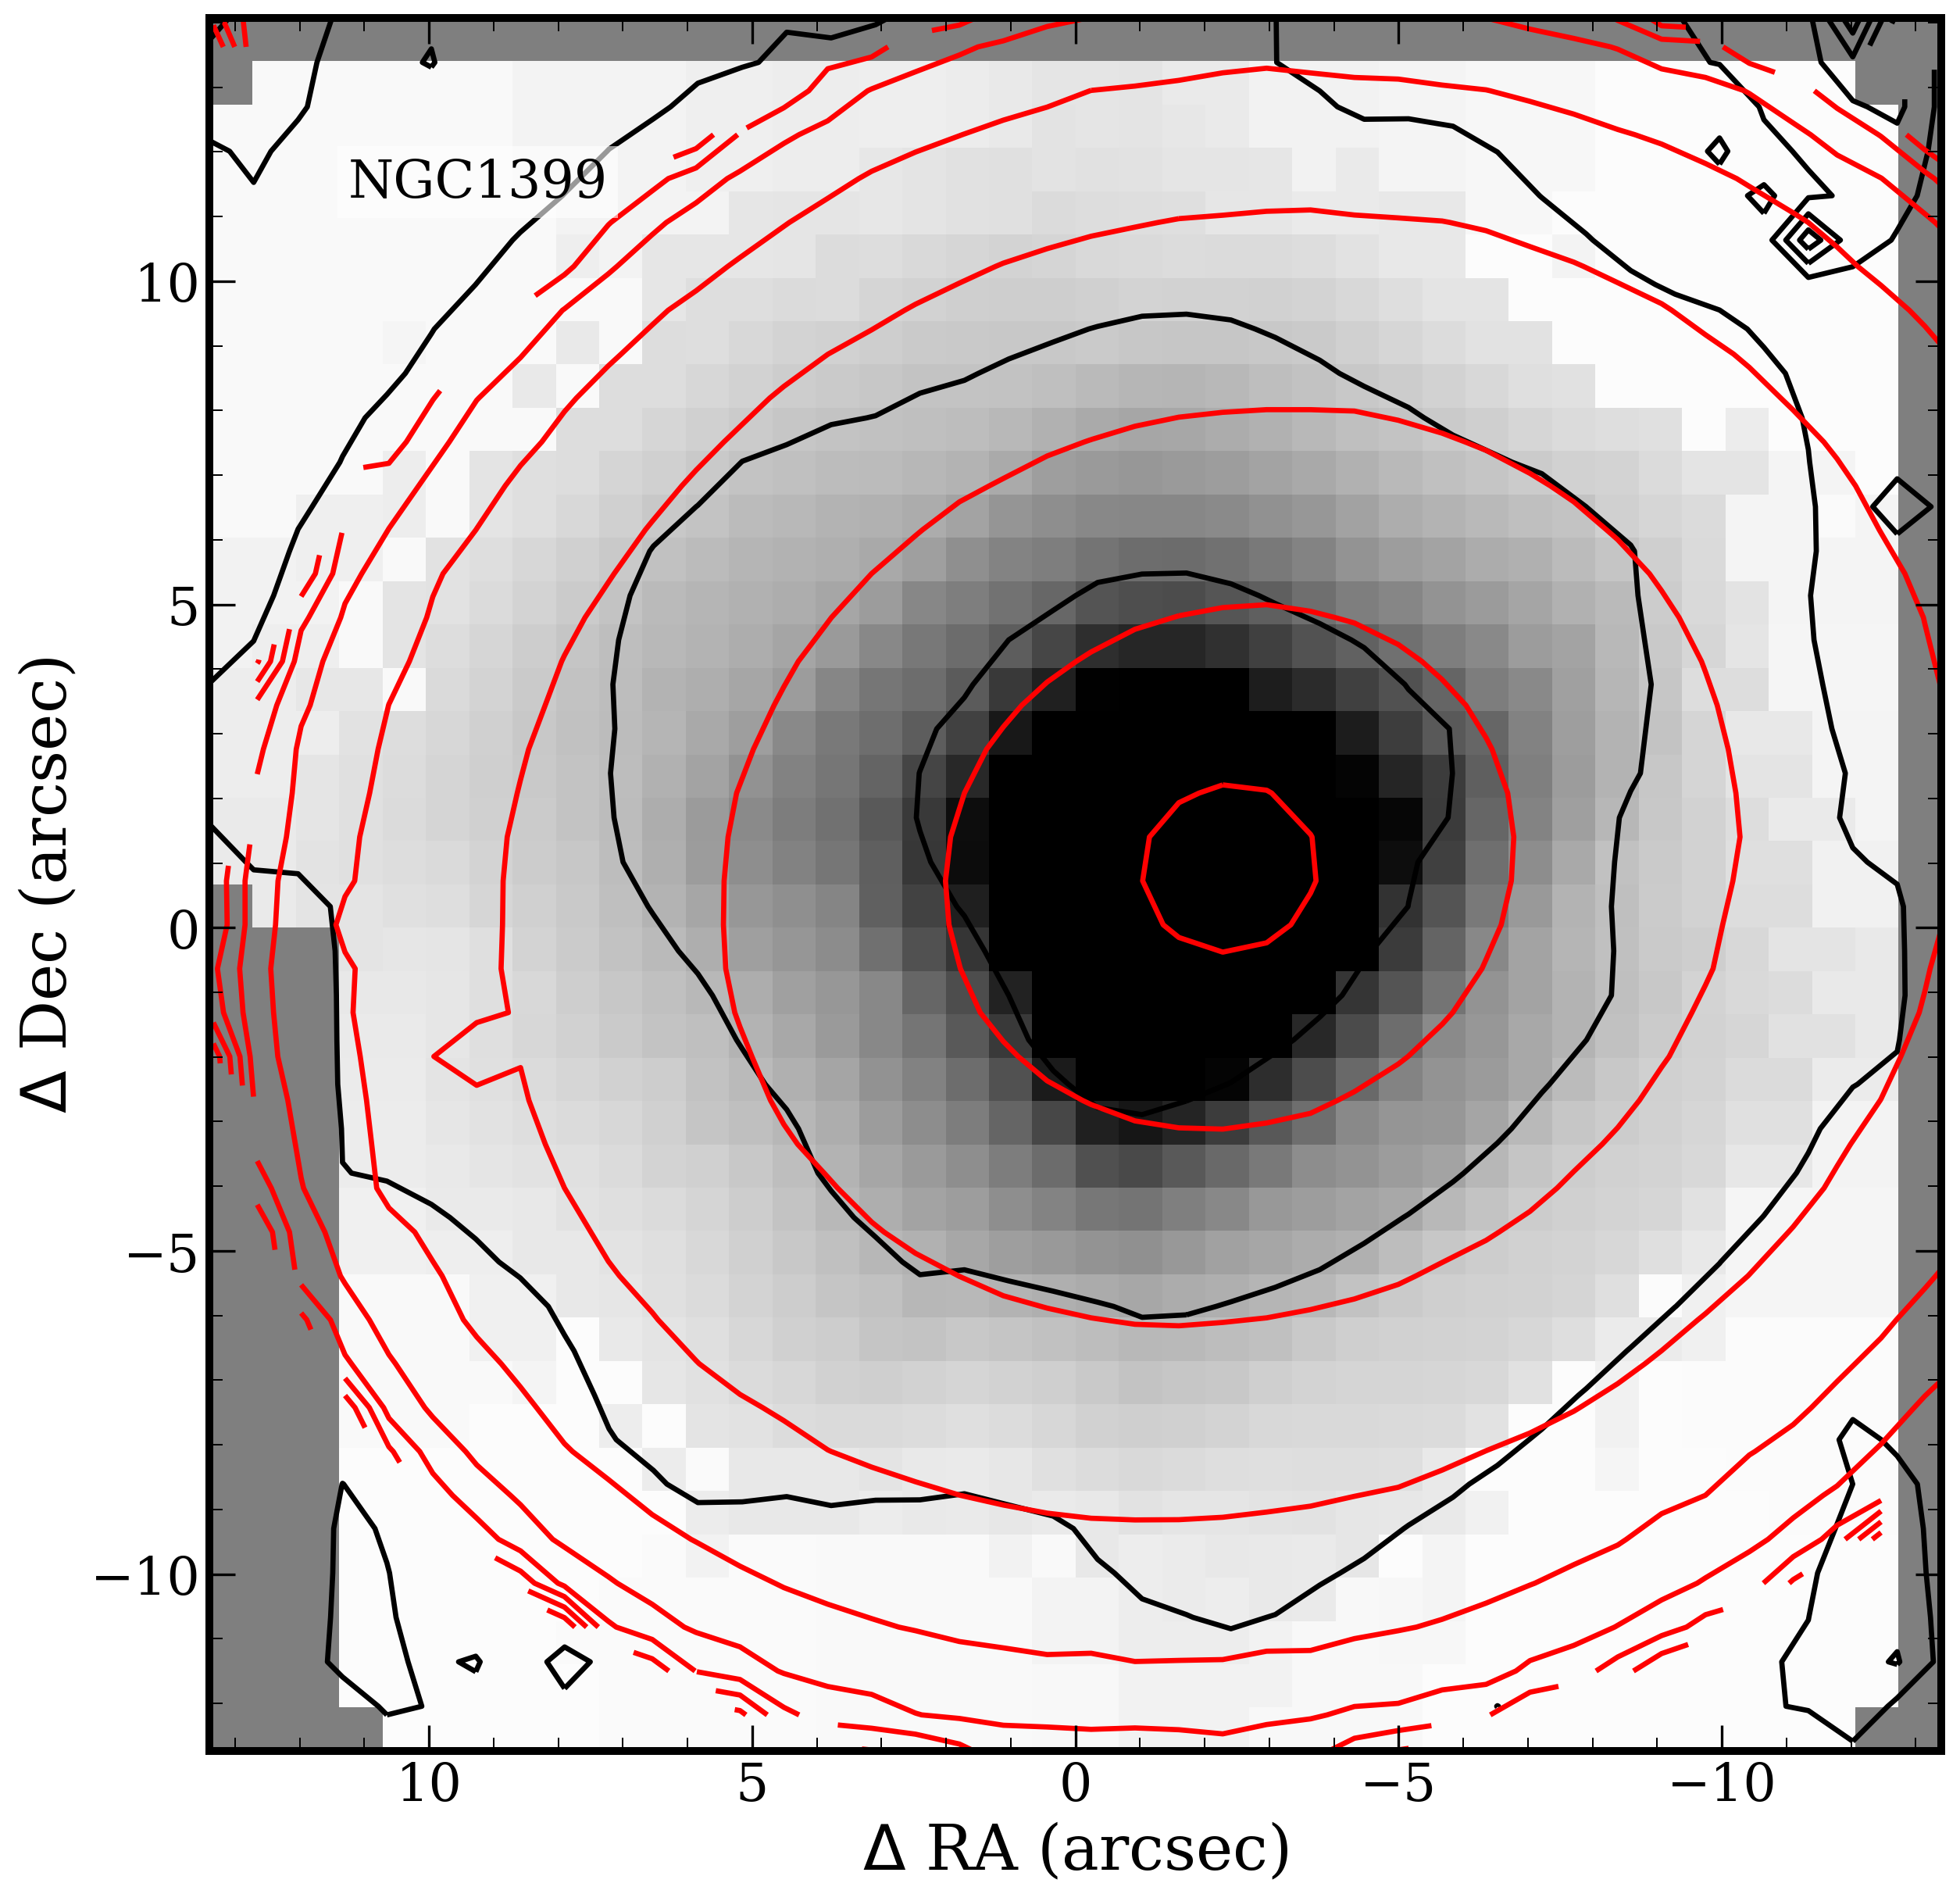
\includegraphics[width=.4\textwidth]{chapter2/hst_vimos_ngc1399.png}
			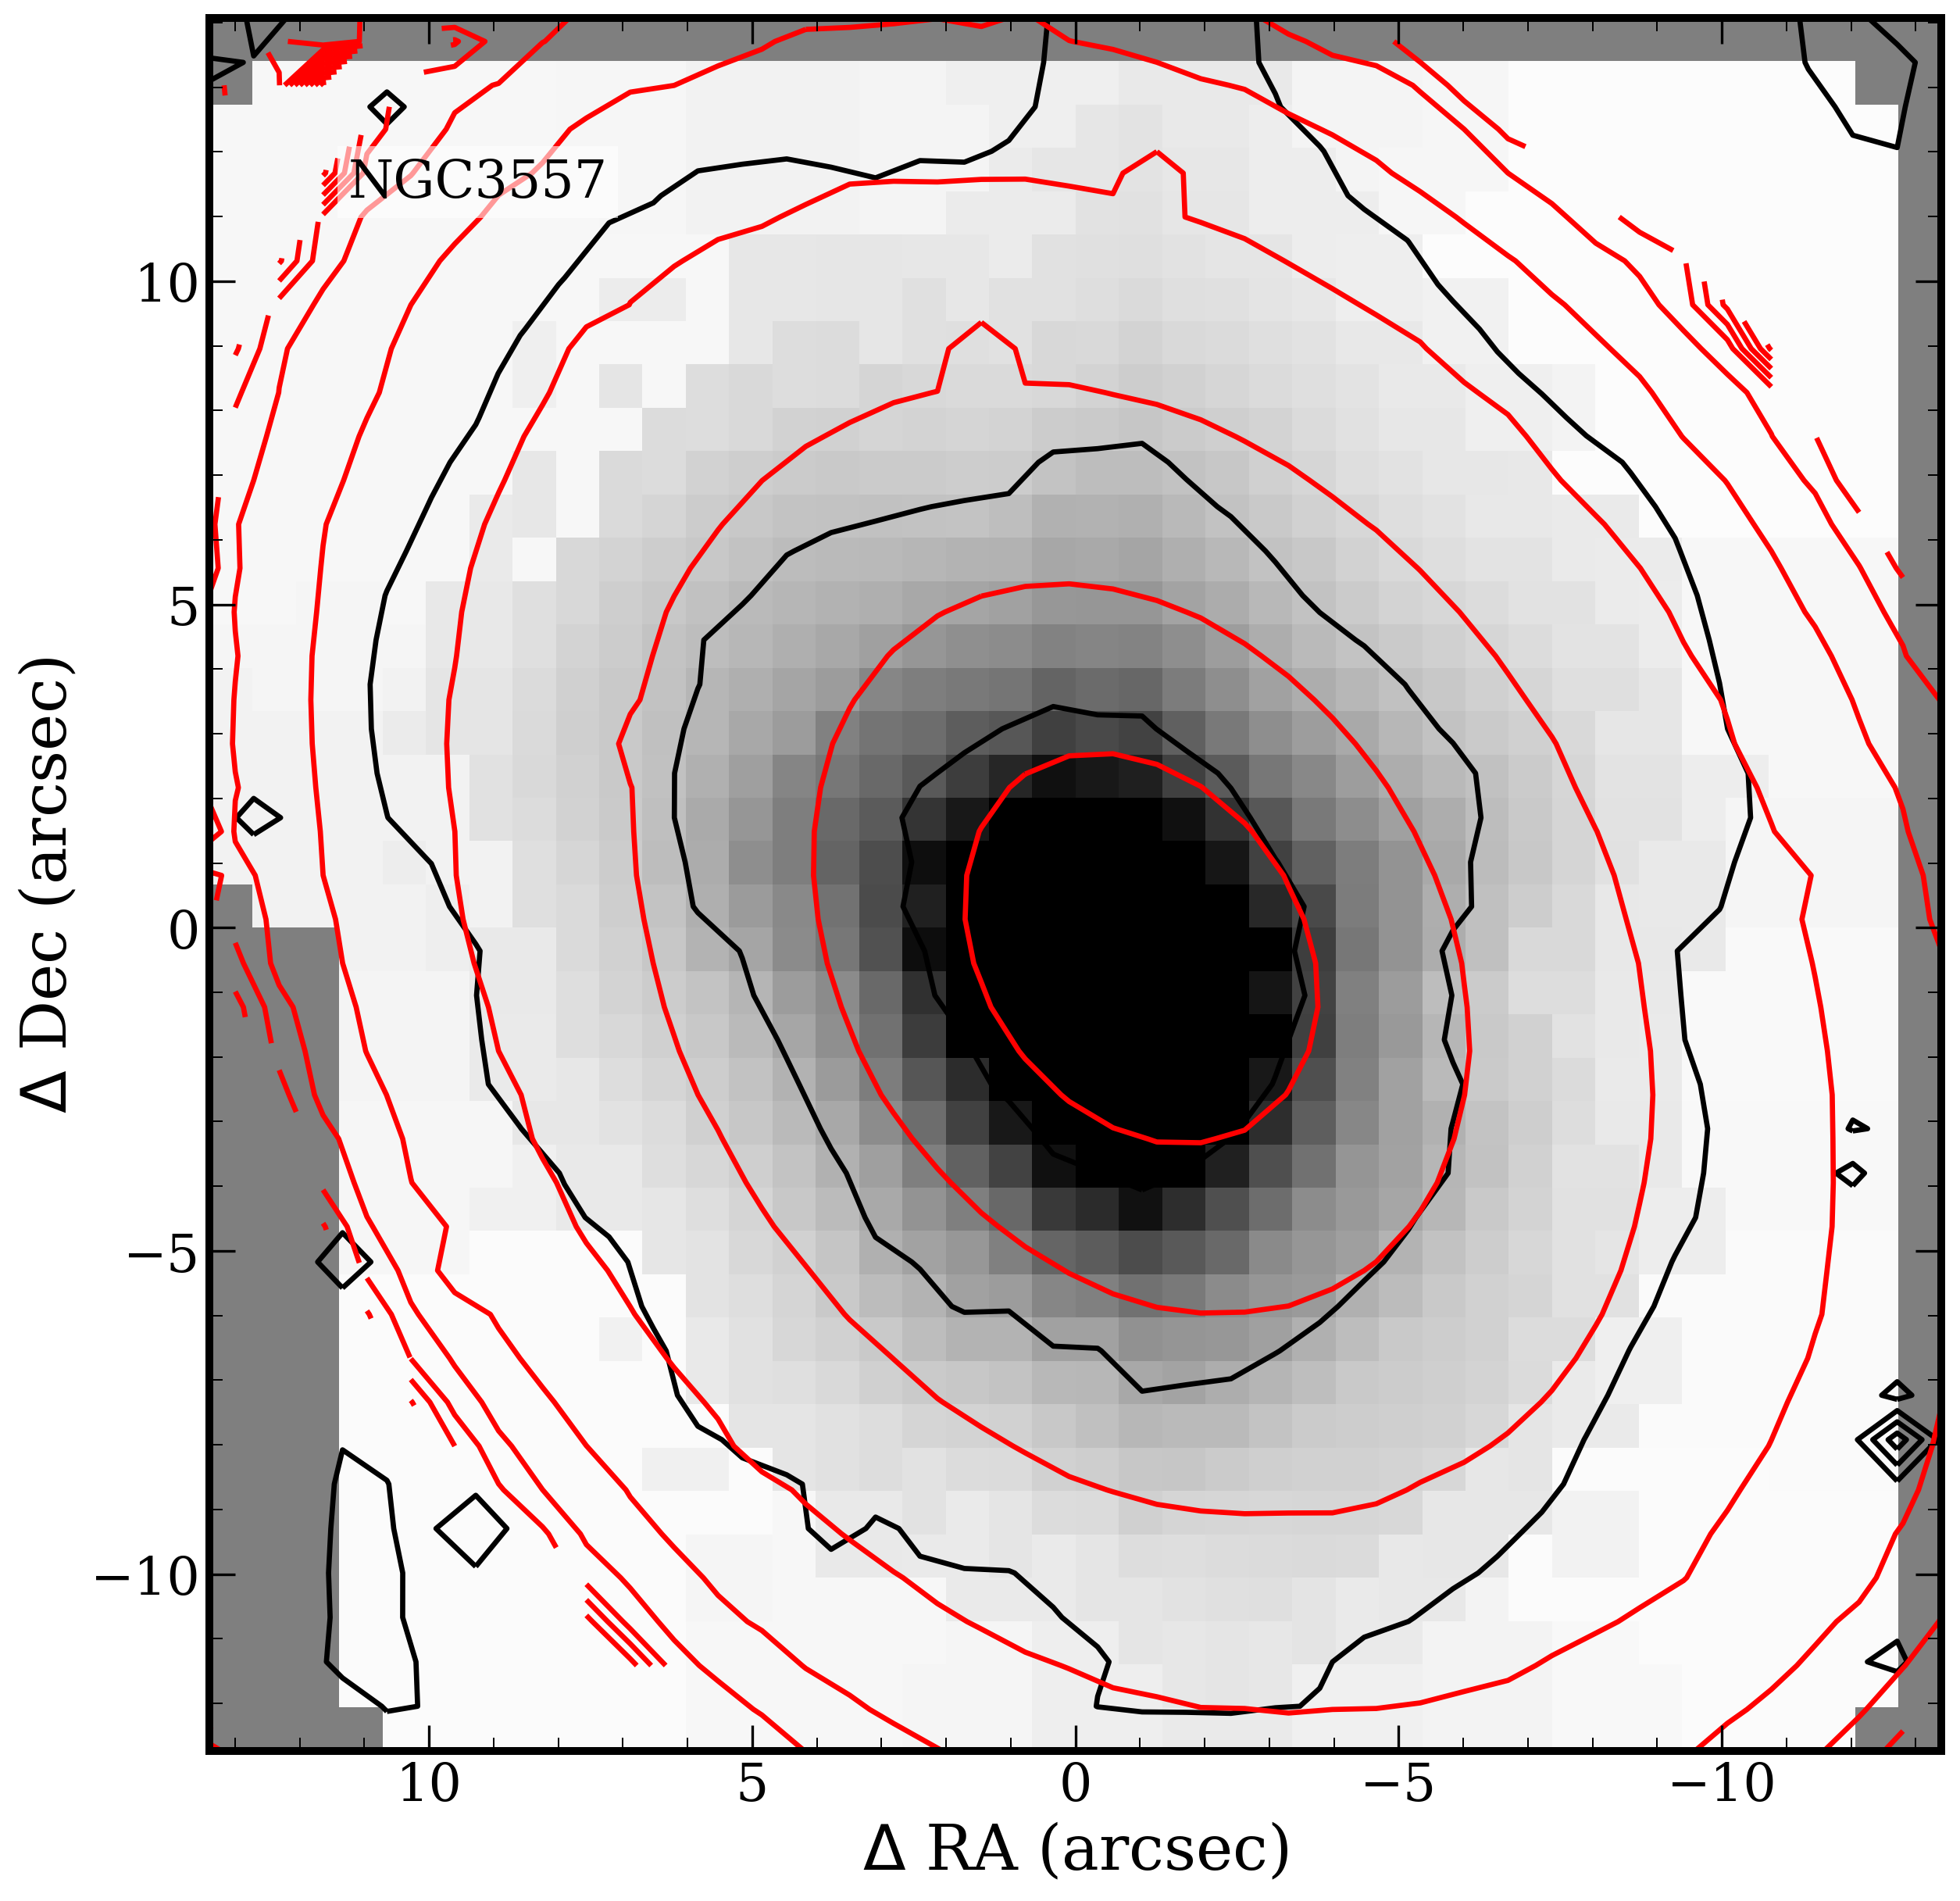
\includegraphics[width=.4\textwidth]{chapter2/hst_vimos_ngc3557.png}
			\caption[Comparison of VIMOS images to \textit{HST}]{Comparison of reconstructed VIMOS image to \textit{HST} image. Clockwise from top left: IC 1459, IC 4296, NGC 3557, NGC 1399. Image and black contours show the VIMOS reconstructed image. Red contours show the \textit{HST} image, reduced to the resolution of VIMOS. All contours are spaced at intervals of 1 mag.}
			\label{fig:HSTvsVIMOS}
		\end{figure}

		The correction spectra found in the process of removing the fringe-like pattern above introduces spatial covariance by effectively applying a spatially smoothing of the data over a scale of 2--3 spaxels. However the effect should not be large, however, so we chose to neglect these correlations and scale the variance spectra by the same factors as the observed spectra. This smoothing is, however, particularly undesirable at the centres of our sample galaxies, where the impact of active galactic nuclei (AGN) should be observed. This should be taken into account later, particularly in Chapter \ref{cha:gas}.

		Finally, in Fig.\,\ref{HSTvsVIMOS} we compare the reconstructed image to \textit{Hubble Space Telescope (HST)} archival images for the four galaxies for which such data existed (IC 1459, IC4296, NGC 1399 and NGC 3557). The \textit{HST} contours (red) are much smoother than the VIMOS contours (black), despite the resolution of the \textit{HST} images being reduced to that of VIMOS. Except for IC 1459 (top left), the VIMOS contours have a characteristic diamond shape due to the poor calibrations between quadrants, which is not seen in the \textit{HST} contours. As stated above, IC 4296 and NGC 1399 are the VIMOS datacubes most effected by the poor quadrant calibrations, while IC 1459 is one of the least effected.

		


	\subsection{Other VIMOS Pipelines}
		\label{subsec:Other}
		Two other publicly available data-reduction pipelines exist for VIMOS. First, the ESO supplied VIMOS pipeline recipe, a plug-in for ESO's general purpose data handling tool \textsc{Gasgano}\footnote{\url{http://www.eso.org/sci/data-processing/software/gasgano}} \citep{Izzo2004, ESO2012}. At the start of this project, this pipeline was not well received by the community. Indeed, ESO's support team suggested I try the alternative pipeline, \textsc{P3D}. Upgrades have since been made to both the instrument and the pipeline, as well as improved suggestions for the observing strategies (OBs), that are meant to remove some of the calibration issues discussed here. However, given the periods when all data were obtained, we have nevertheless decided not to experiment with this tool.
		
		% No publication paper for IDL? Is this because it is commerical?
		Second, \textsc{P3D}\footnote{\url{http://p3d.sourceforge.net/}} is a comprehensive, multi-instrument package with both a decent graphical user interface (GUI) and an application programming interface (API) in the commercial \textsc{Interactive Data Language}\footnote{\url{http://www.harrisgeospatial.com/SoftwareTechnology/IDL.aspx}} (\textsc{IDL}) \citep{Sandin2010, Sandin2011}. It includes routines for all the standard reduction steps: bias subtraction, tracing of the fibres along the dispersion axis, flatfielding, wavelength calibration, flux calibration, cosmic-ray removal and DAR correction. It also combines the quadrants into a single FITS file, although as mentioned above the flux calibration of the different quadrants is attempted by comparing the intensities of the blended sky line at 5199\,\AA. In our case, this calibration step failed for most galaxies as the 5199\,\AA\ sky line is extremely faint (or not detected) in many of the exposures. This failure can be seen in the extremely sharp offsets between the quadrants on the left and right of the reconstructed image shown in the left panel of Fig.\,\ref{fig:P3D}. 

		\begin{figure}
			\centering
			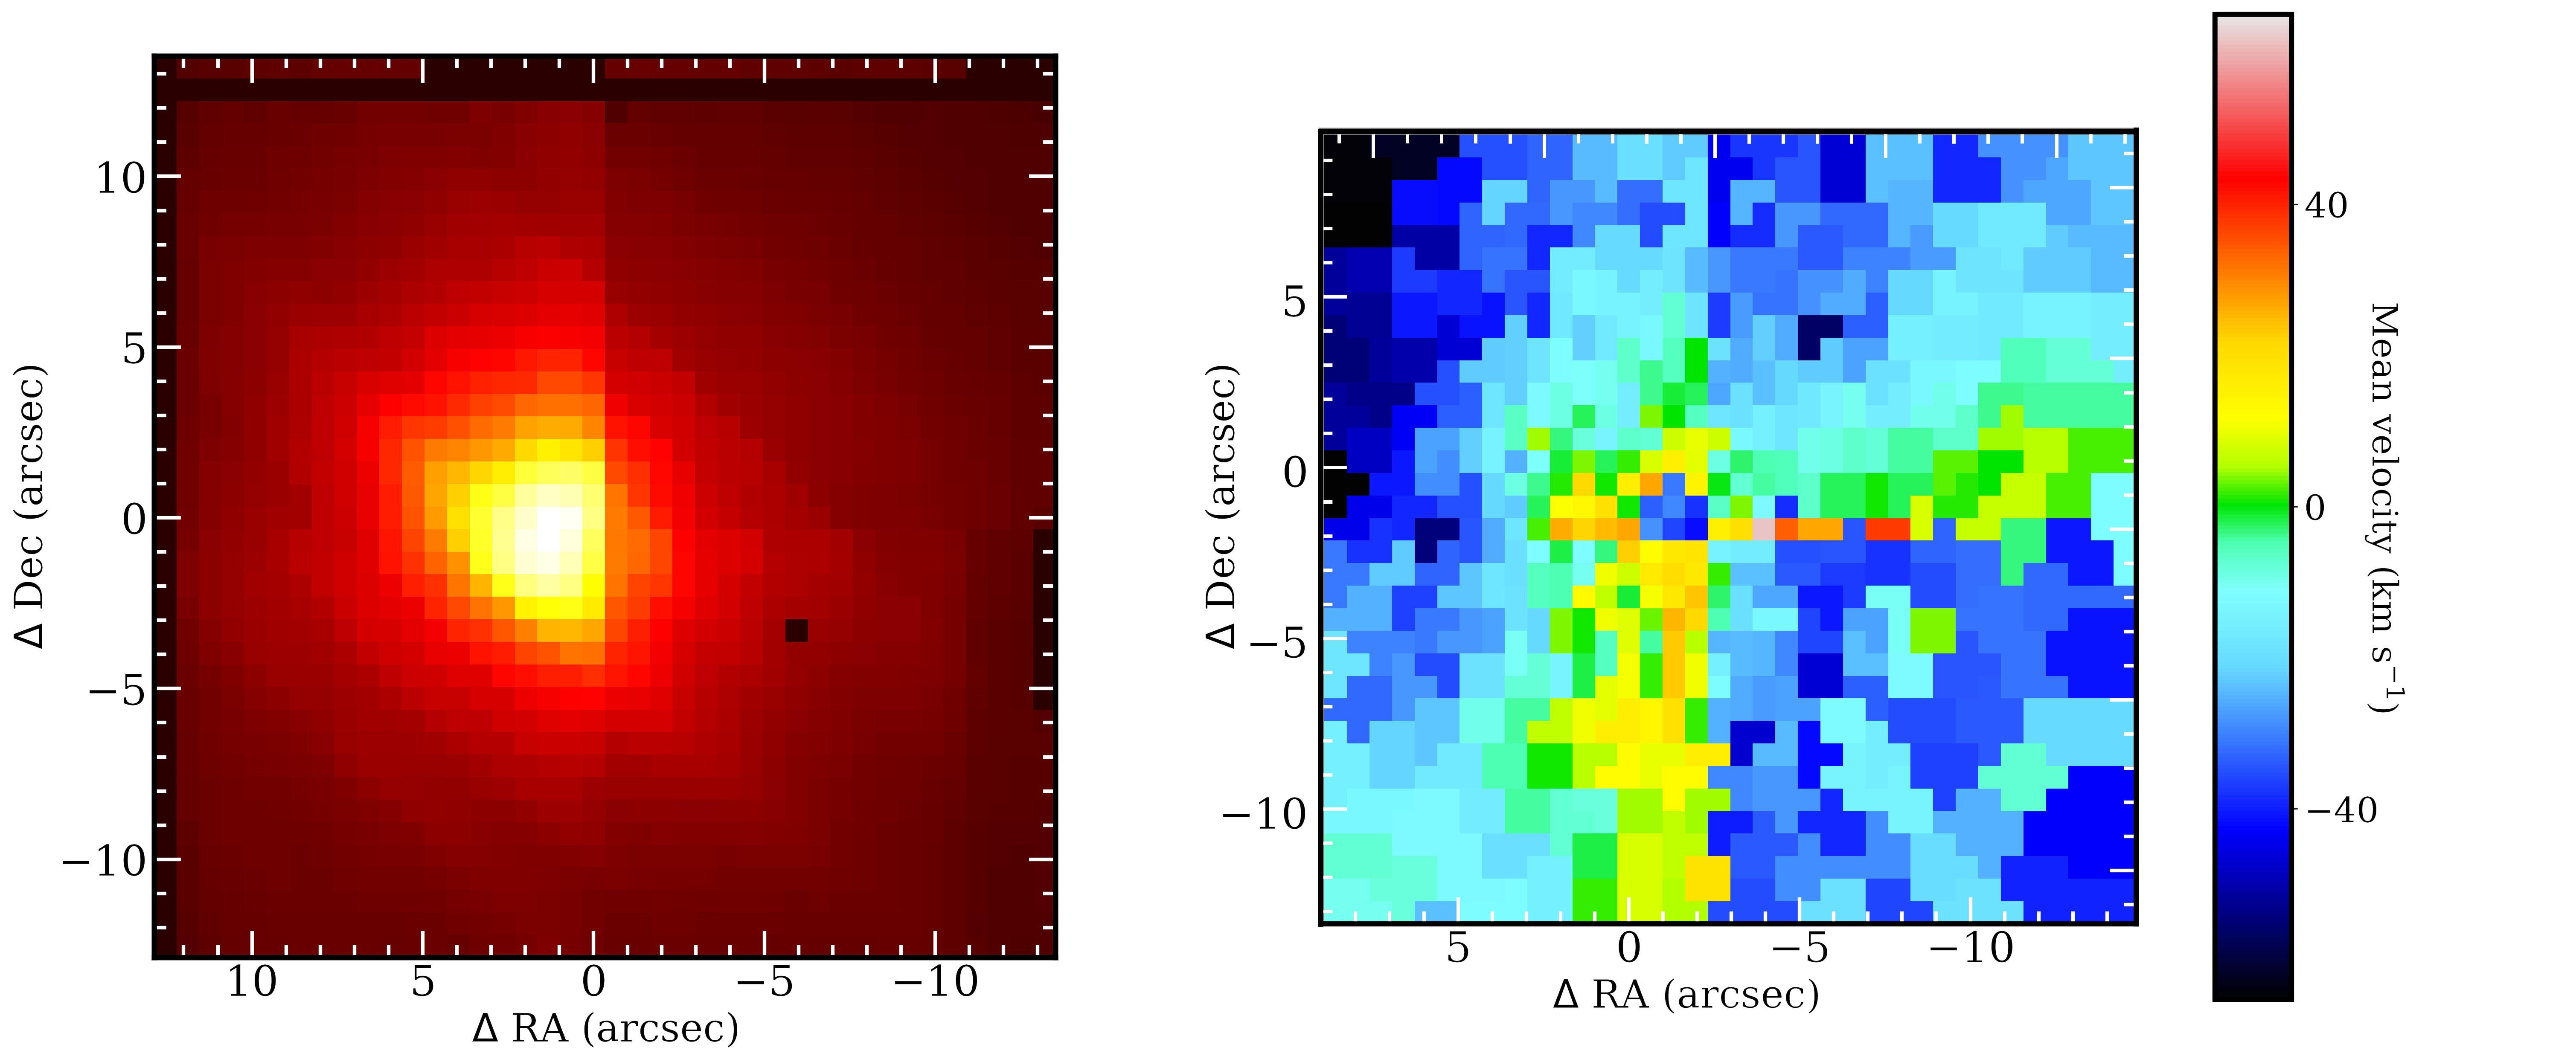
\includegraphics[width=.9\textwidth]{chapter2/P3D_NGC1399.png}
			\caption[\textsc{P3D}-reduced data problems]{Examples of problems with \textsc{P3D}-reduced data. Left panel: flux map (reconstructed image) of NGC 1399 Right panel: mean stellar velocity map of NGC 1399. Both maps show sharp offsets between the quadrants. The outer 2 spaxels on all sides of the velocity map were discarded.}
			\label{fig:P3D}
		\end{figure}


		The \textsc{p3d} wavelength-calibration step was not very successful either, as sharp offsets remain between the quadrants in the spectral direction. While this was still the case with \textsc{Py3D}-reduced data, the issue was much worse and more prevalent for \textsc{P3D}-reduced data. For example, the right panel of Fig.\,\ref{fig:P3D} shows the mean stellar velocity map of NGC 1399 extracted from \textsc{P3D}-reduced data. The wavelength calibration is so poor that the rotation pattern of the galaxy is completely obfuscated.

		
\section{Multi-unit Spectroscopic Explorer (MUSE)}
	\label{sec:MUSE}

	\subsection{MUSE Instrument}
		The Multi-unit Spectroscopic Explorer (MUSE) is located on UT4 of ESO's VLT \citep{Bacon2010}. It is comprised of 24 channels, each feeding an IFU (image slices) and spectrographs for a total contiguous field of view of $1\arcmin \times 1\arcmin$ at spatial sampling of $0\farcs2$. It has a spectral range of 4800-9300\,\AA\ with a spectral resolution of $\approx 2.3$\,\AA\ sampled at 1.25\,\AA\,pix$^{-1}$. MUSE is currently offered with and without adaptive optics (AO), and a narrow-field mode (with an order of magnitude improvement in spatial resolution and sampling) is planned for the future. 
		
	\subsection{MUSE Archival Observations}
		Four of the sample galaxies are in the MUSE archive: IC 1459, IC 4296, NGC 1316 and NGC 1399. NGC 1316 (observed as part of programme 094.B-0298A) and NGC 1399 (programme 094.B-0903A) were both observed as mosaics, while IC 1459 and IC 4296 (both also programme 094.B-0298A) were observed in single pointings. All were observed in service mode during ESO period 94, in the MUSE wide-field mode without adaptive optics. Every OB in both programmes followed the standard MUSE calibration plan.

	\subsection{MUSE Data Reducing}
		\label{subsec:MUSEreduction}
		
		Because the computing resources required to reduce raw MUSE data are very large (the recommended system configuration for the reduction of a single-pointing OB of 5 exposures is: 64\,GB of memory, 24 CPU cores and 4\,TB of free disk space), the data quality is high, and the pipelines products are known to be robust, we adopt for this project the pre-reduced (known as Phase 3) data products from ESO, so that the ESO data reduction pipeline\footnote{\url{http://www.eso.org/sci/software/pipelines/muse/muse-pipe-recipes.html}} is already applied. 

		The ESO pipeline contains all standard IFU data reduction steps: bias subtraction, flatfielding of detectors using continuum lamp exposures, flatfielding of fibres using twilight exposures, wavelength calibration, flux calibration using standard stars and sky subtraction (both programmes included dedicated sky exposures). Tiled observations, where present, are combined into a final mosaic.

		We found that the Phase 3 data products were indeed generally of a sufficient quality for our purposes, except that in both IC 1459 and IC 4296 the sky appears to have been over-subtracted. The ESO Phase 3 data release description for MUSE\footnote{\url{https://www.eso.org/sci/observing/phase3/data\_releases/IDP\_MUSE\_IFU\_release\_description\_1.0.pdf}} points out that the automatic data-reduction routine does not verify stable conditions (such as photometry and moon visibility) before applying the sky subtraction. Unstable conditions may well be the source of over subtraction which manifested itself as enormous apparent absorption features (often with negative fluxes) in the spectra. To remove this over-subtraction, we developed our own pseudo-sky subtraction routine. A median spectrum was taken from four $20 \times 20$\,spaxel regions, one in each spatial corner of the ESO reduced cube. After checking that no stellar continuum could be fit to the medium sky spectrum (i.e.\ that very little light from the galaxy is contaminating the pseudo-sky regions), this median sky spectrum was subtracted from each spaxel in the cube. 

		This extra (pseudo-)sky subtraction was not possible for NGC 1316 and NGC 1399 due to mosaic nature of the observations, since this sky subtraction should be applied to each exposure of the mosaics independently (while the different exposures are already combined as part of the automated data reduction). It is also impossible to access data products from intermediate steps in the data-reduction process, such as immediately before the mosaic is produced. Fortunately, both NGC 1316 and NGC 1399 are not as badly affected by poor sky subtraction as IC 1459 and IC 4296, so they are left uncorrected. 

		Finally, we trimmed all the cubes to the central $30\arcsec \times 30\arcsec$ ($150 \times 150$\,spaxels) only, to (a) avoid the regions used for the pseudo-sky spectrum and (b) reduce the computing resources required for spatial binning (see Section \ref{sec:analysis}). In any case, the bins would be so large in the outer parts as to be effectively useless (see Fig\,\ref{fig:egSNR}).

		As for the VIMOS data, the variance spectra are propagated throughout the entire data-reduction pipeline, including our additional pseudo-sky subtraction step, and are squared-rooted at the end, to be used as noise inputs at the analysis stage. 

		\subsubsection{MUSE Data Quality}
			As with the VIMOS data, we here (Fig.\,\ref{fig:HSTvsMUSE}) examine the reconstructed images (image and black contours), with archival \textit{HST} images (red contours). All galaxies in our sample for which MUSE data was available, also had archival \textit{HST} images available too. It can clearly be seen that the MUSE contours well match the \textit{HST} contours, unlike the for the VIMOS data (see Fig.\,\ref{fig:HSTvsVIMOS}). As such, it can be seen that the MUSE data is of a superior quality to the VIMOS data and as such, where both are available, a higher weighting should be given the MUSE data and its derivatives. 

			\begin{figure}
				\centering
				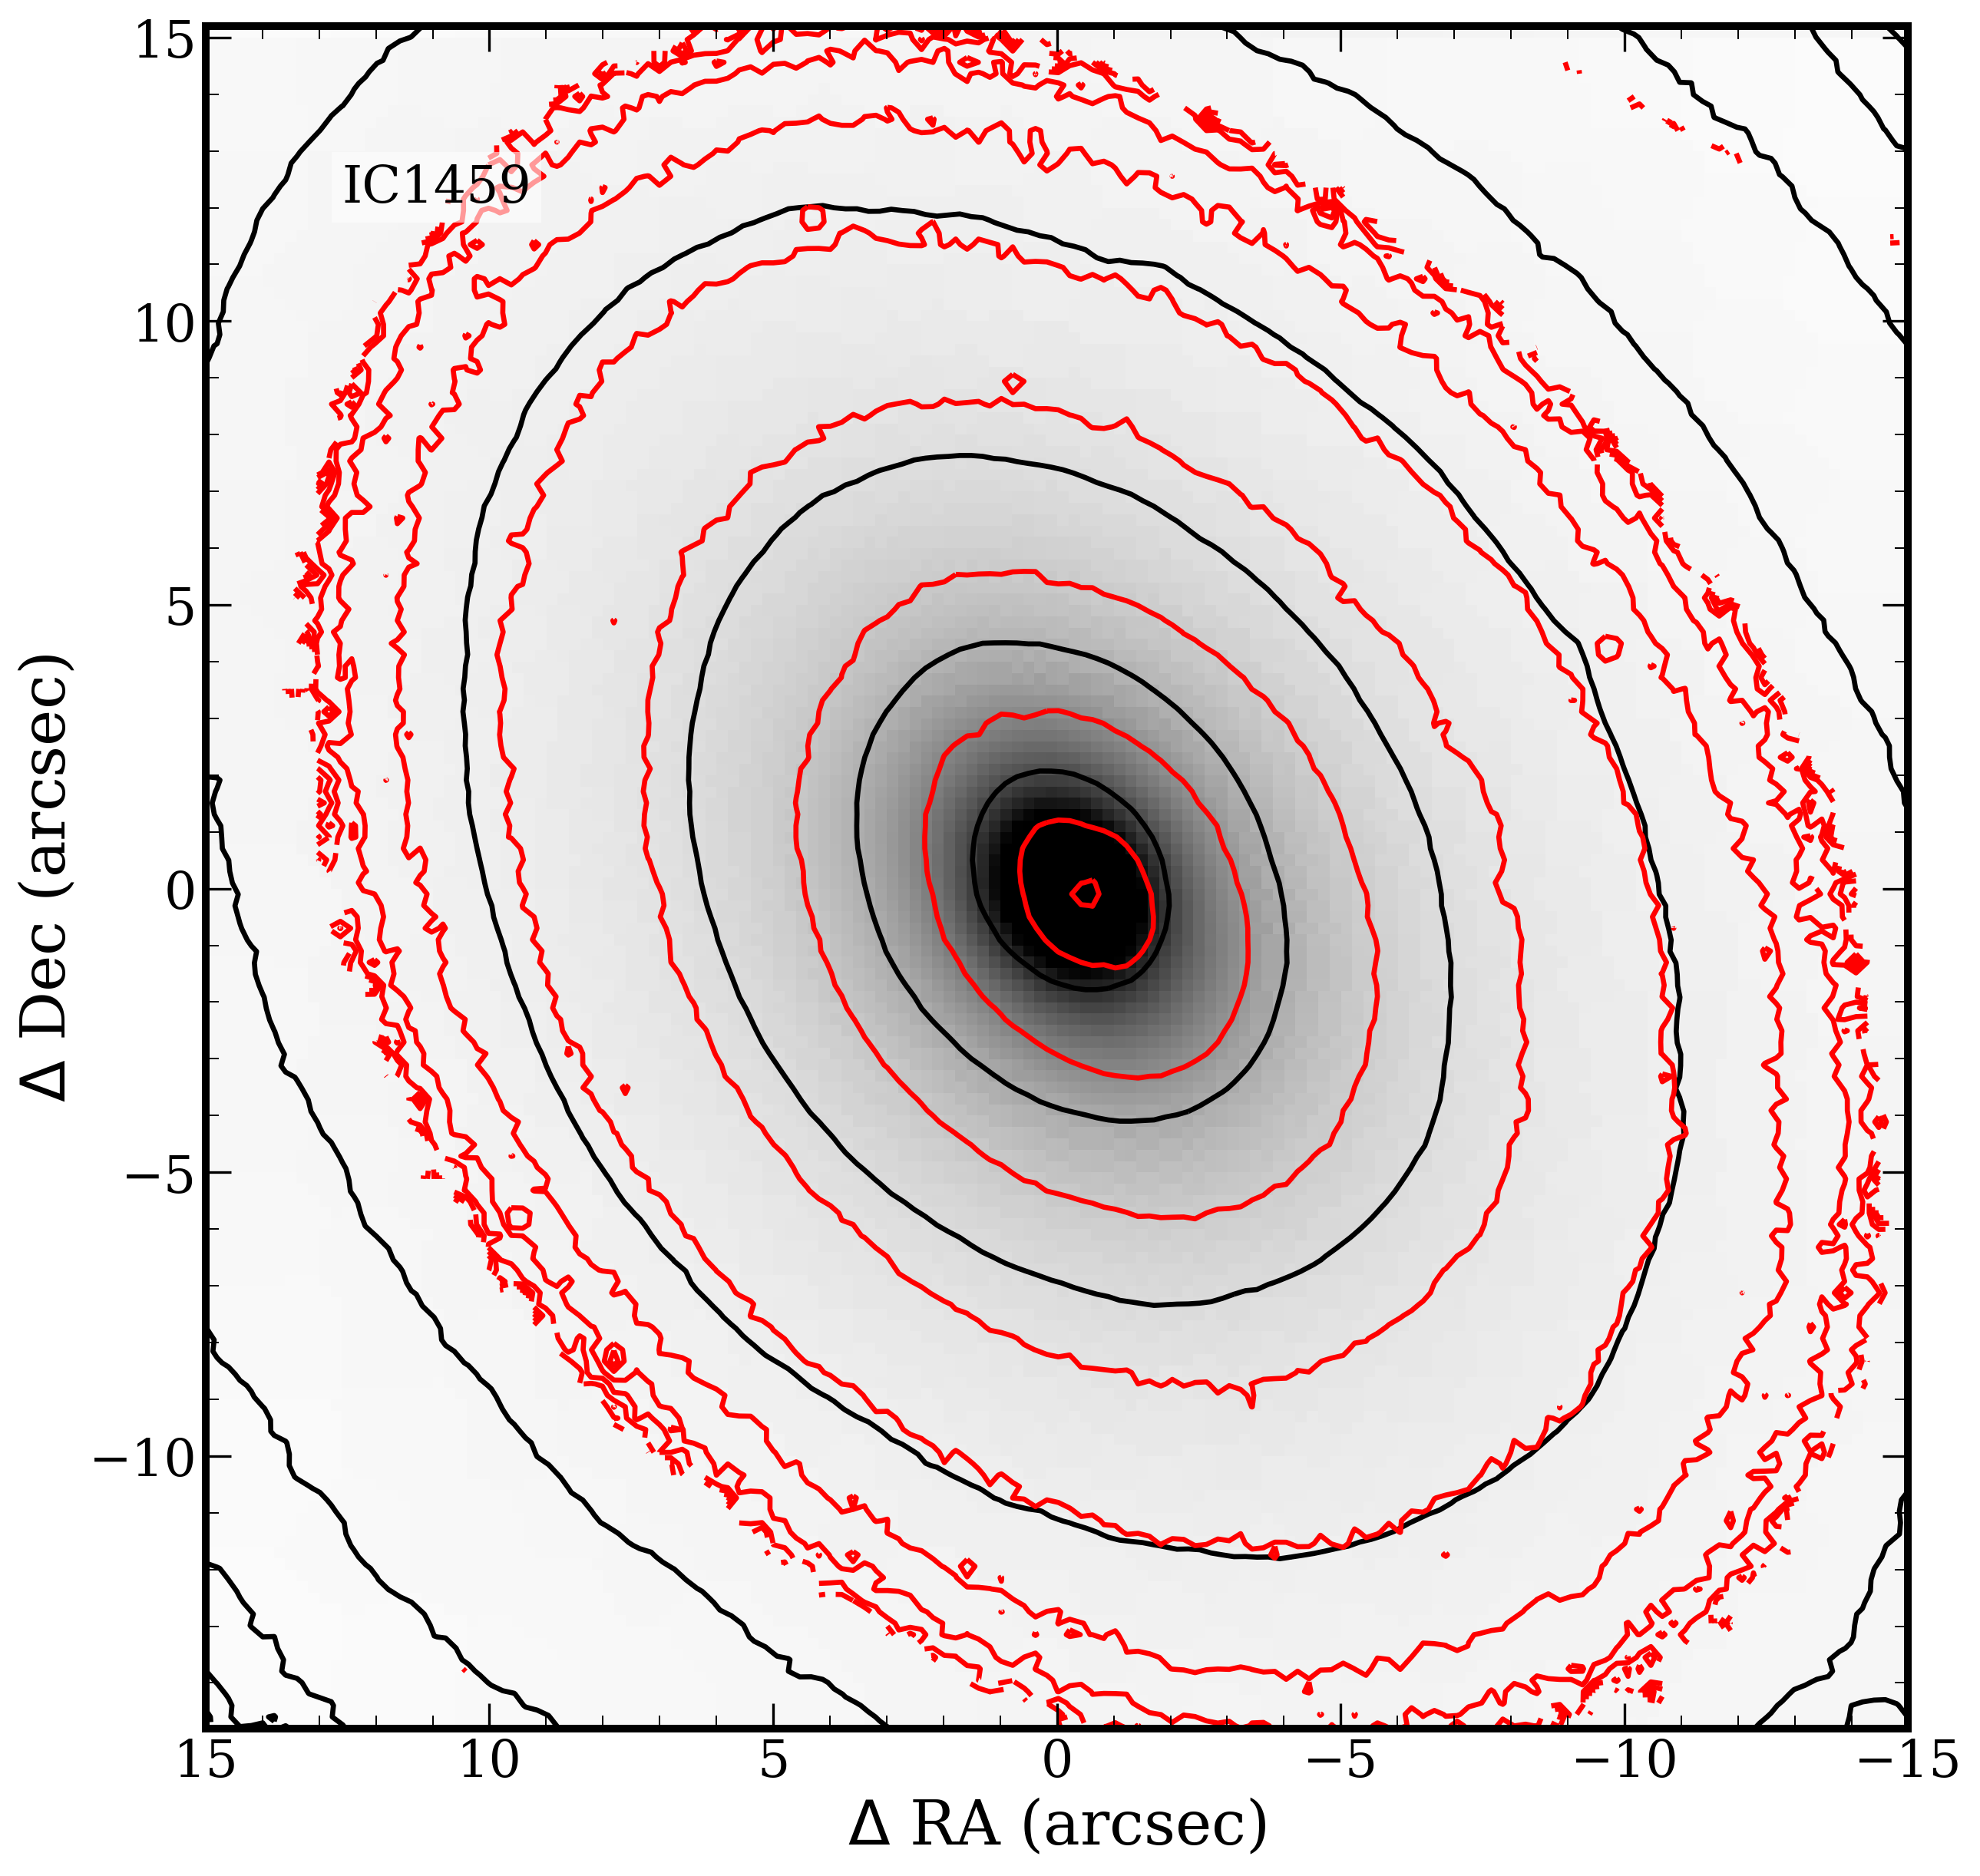
\includegraphics[width=.4\textwidth]{chapter2/hst_muse_ic1459.png}
				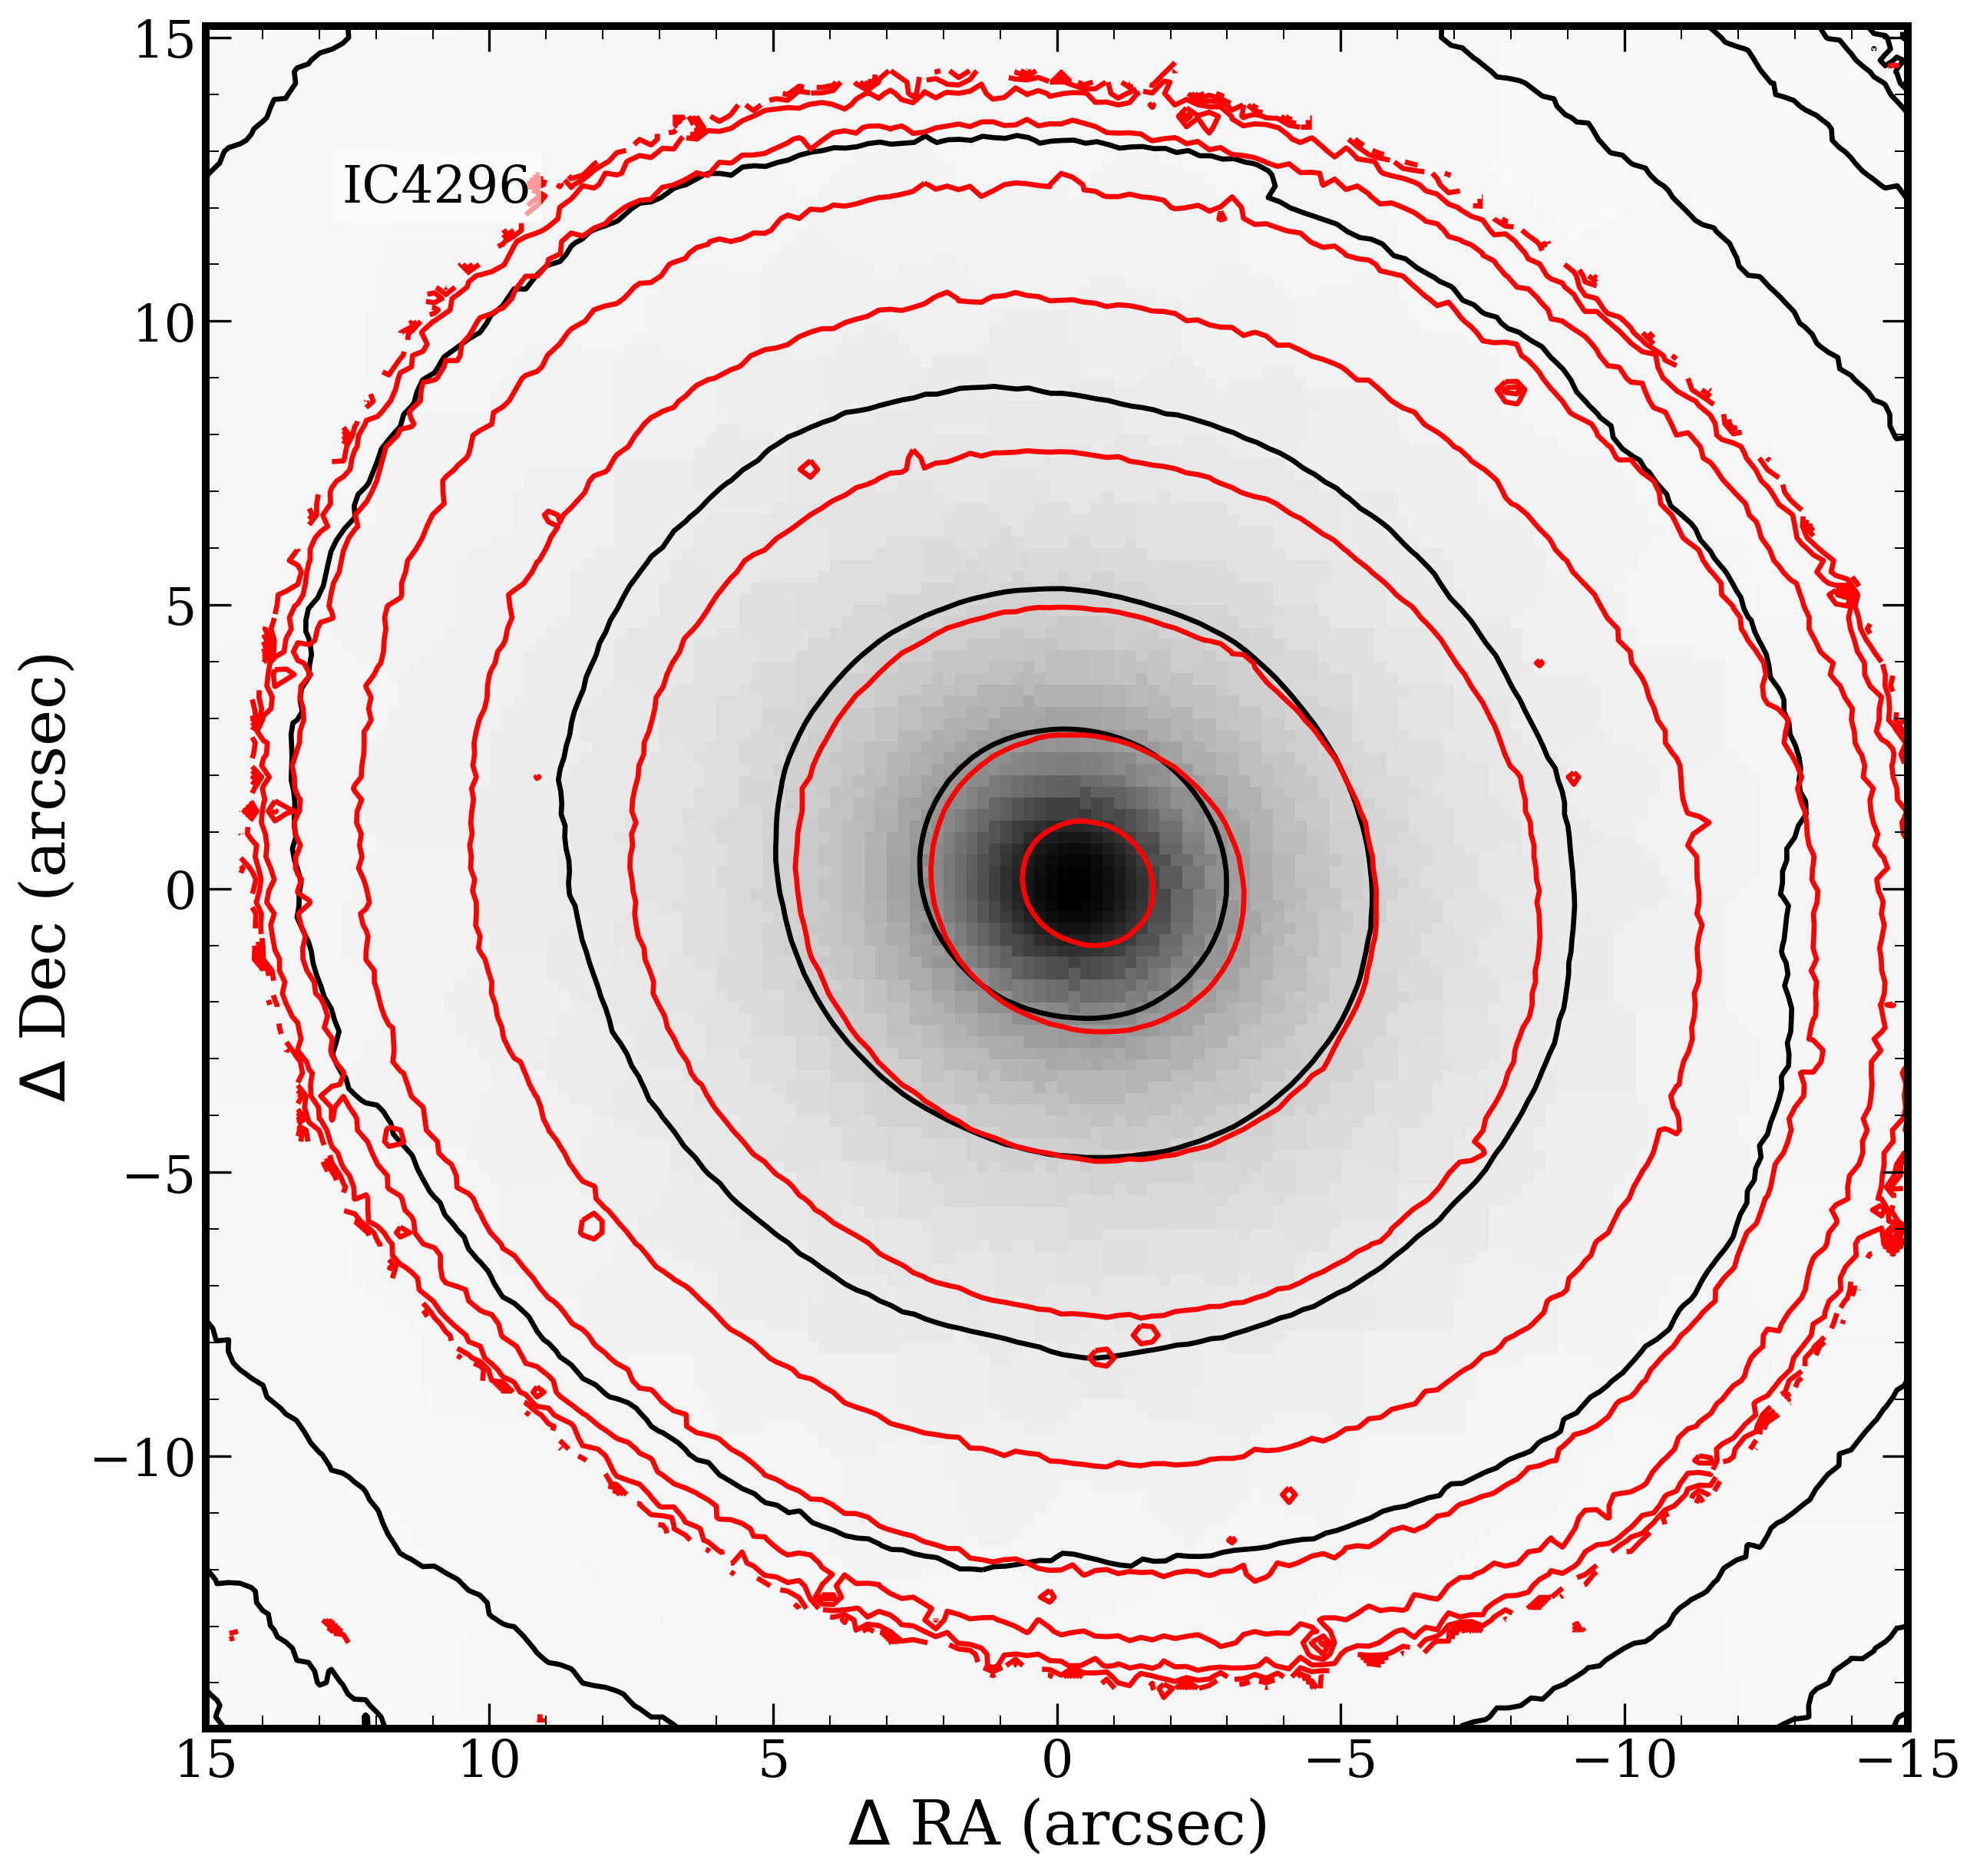
\includegraphics[width=.4\textwidth]{chapter2/hst_muse_ic4296.png}
				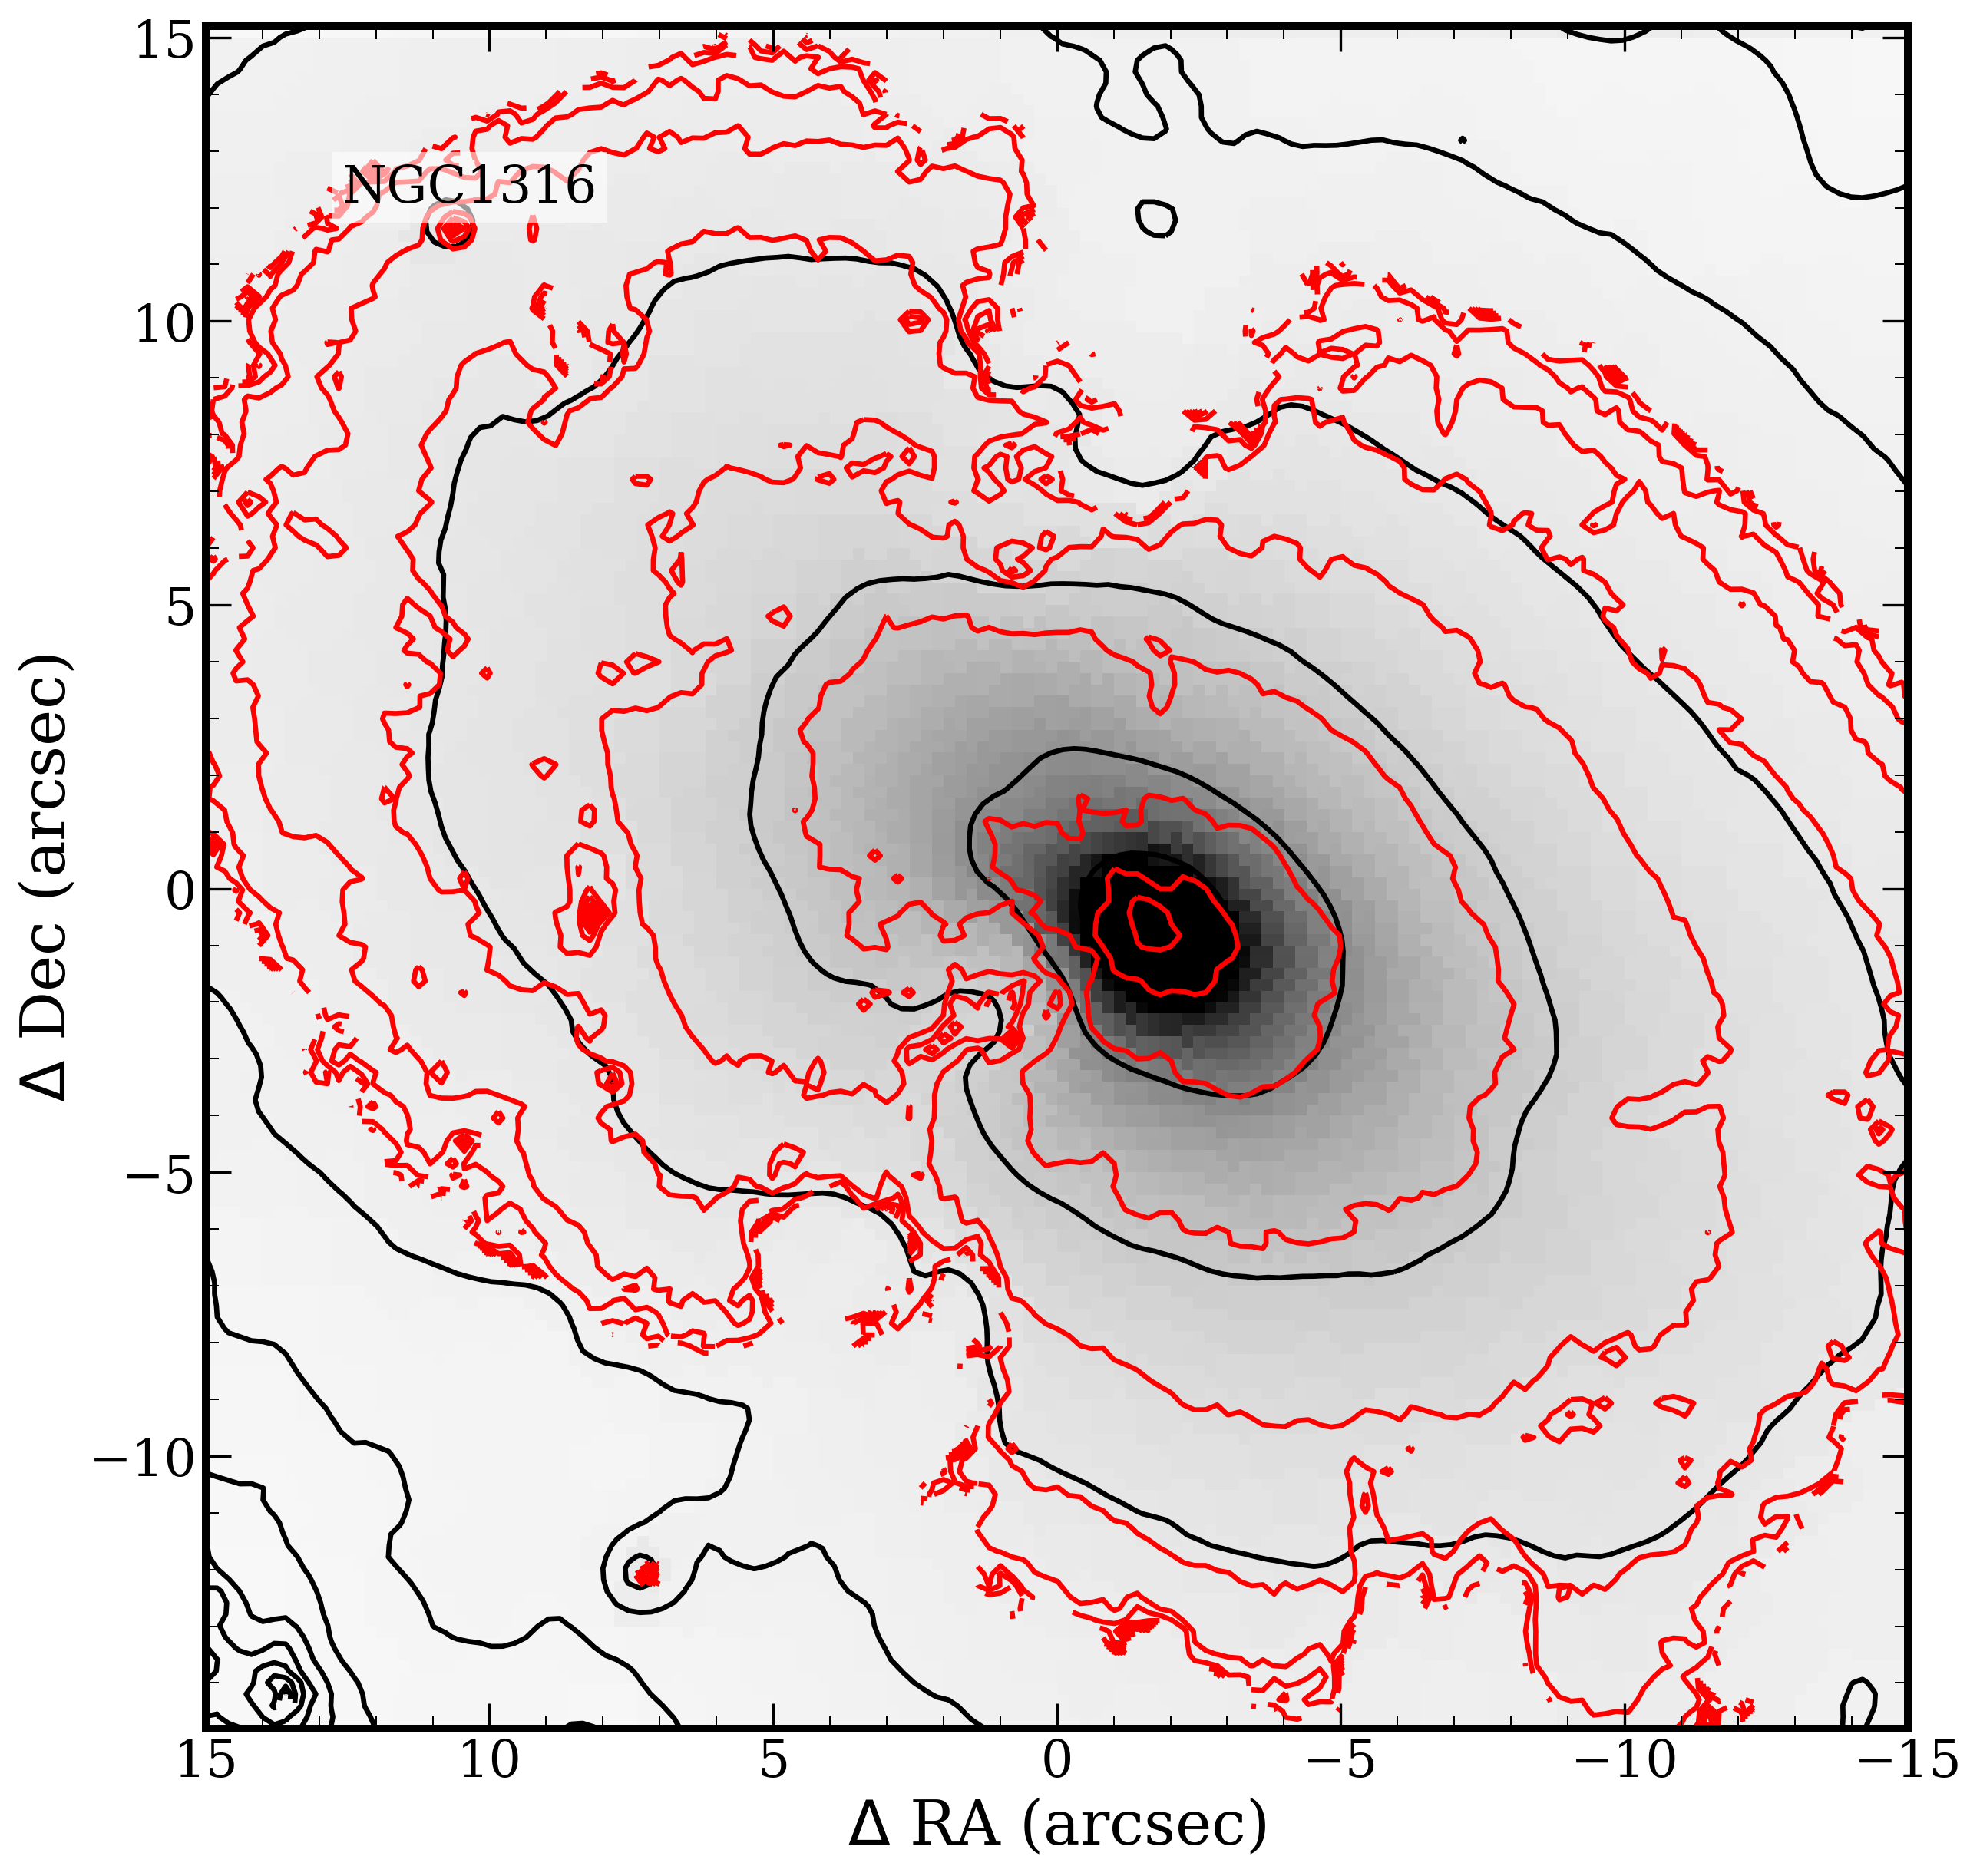
\includegraphics[width=.4\textwidth]{chapter2/hst_muse_ngc1316.png}
				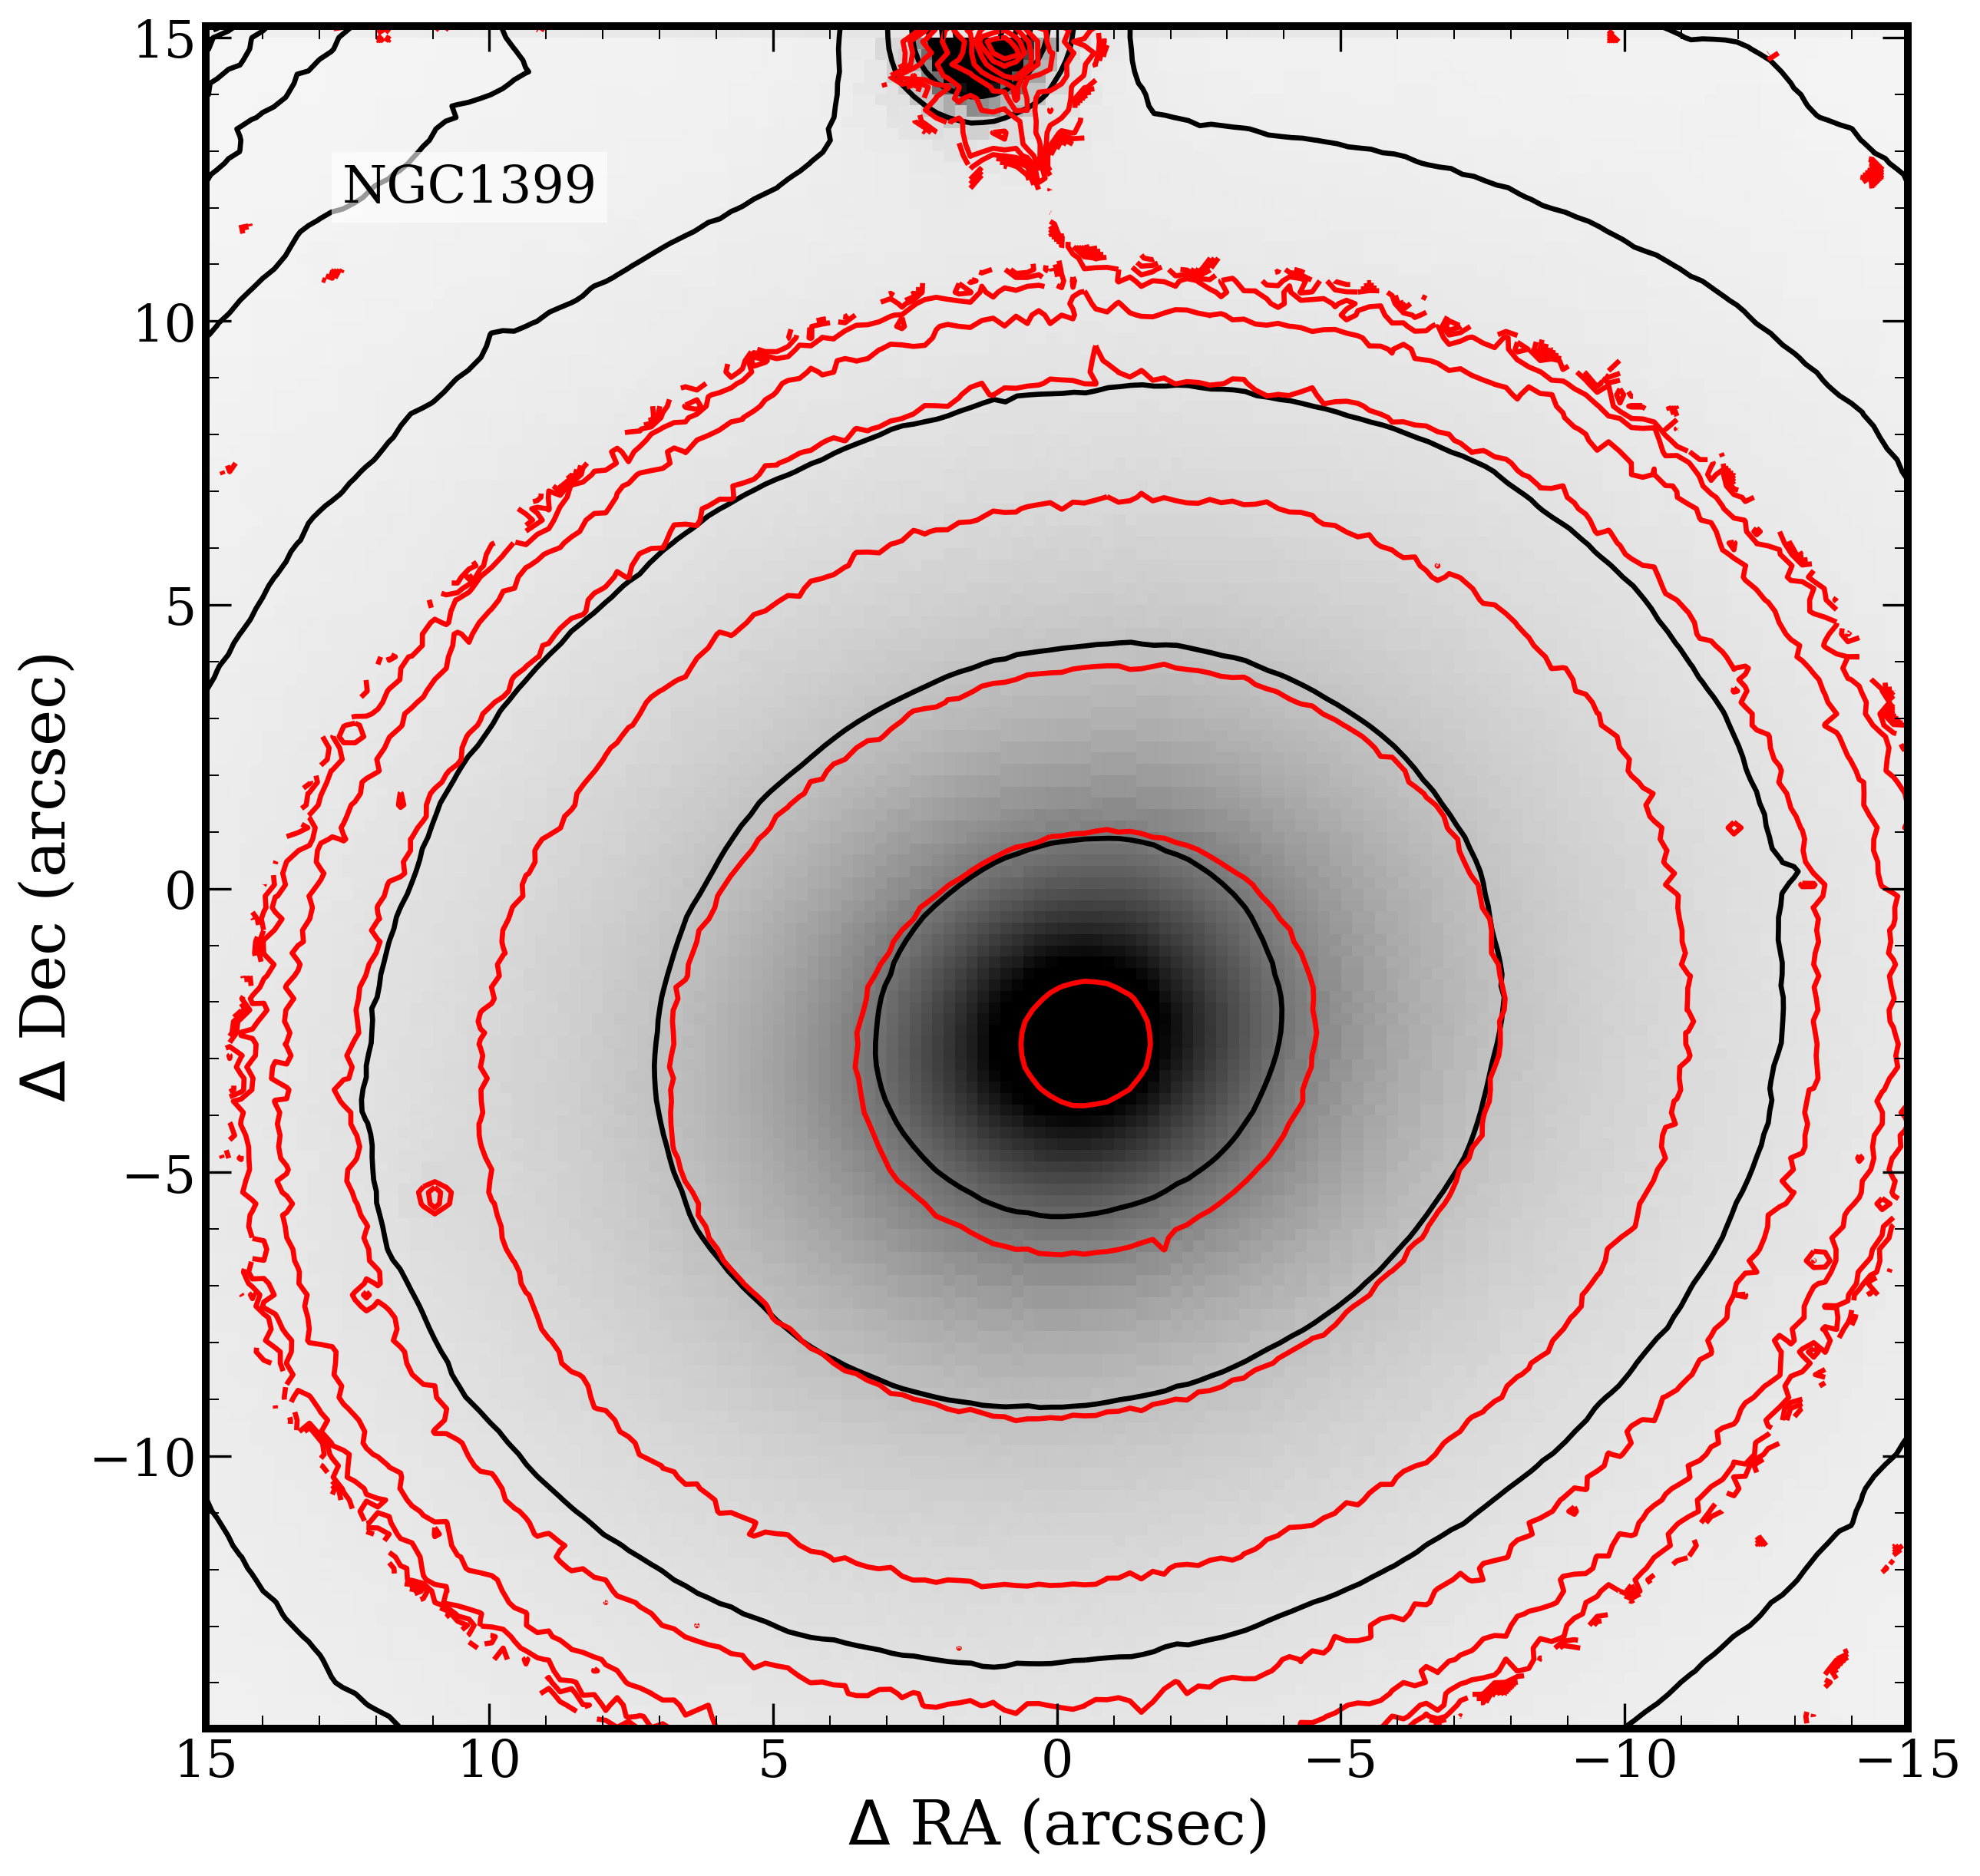
\includegraphics[width=.4\textwidth]{chapter2/hst_muse_ngc1399.png}
				\caption[Comparison of MUSE images to HST]{Comparison of reconstructed VIMOS image to \textit{HST} image. Clockwise from top left: IC 1459, IC 4296, NGC 1316, NGC 1399. Image and black contours show the MUSE reconstructed image. Red contours show the \textit{HST} image, reduced to the resolution of VIMOS. All contours are spaced at intervals of 1 mag.}
				\label{fig:HSTvsMUSE}
			\end{figure}


\section{Data Analysis}
	\label{sec:analysis}
	From this point on, the VIMOS and MUSE datasets are treated almost identically, the only difference (other than the different spectral ranges and resolutions) being that the MUSE datacubes are binned to a higher signal-to-noise ratio (S/N).

	For each galaxy (i.e.\ each combined cube), the data analysis process can be summed up as follows, each step being detailed below:
	\begin{enumerate}
		\item Spatially bin the spectra using Voronoi binning.
		\item Identify the relevant stellar templates, by fitting the entire galaxy spectrum (obtained by summing all galaxy spectra) with all the templates from the Medium-resolution Isaac Newton Telescope (INT) Library of Empirical Spectra (MILES) library, and hereafter using only the non-zero weight templates.
		\item Estimate the redshift and velocity dispersion of the entire galaxy spectrum with an iterative routine. % Markov chain Monte--Carlo (MCMC) routine. 
		\item Find the best-fitting line-of-sight velocity distribution (LOSVD; as parametrised by the Gaussian parameters $v$, the mean velocity and $\sigma$, the velocity dispersion) of the stellar and ionized gas components in each bin, using a Monte--Carlo method to estimate the uncertainties on the measurements. 
		\item Remove the fitted emission lines and measure the absorption line strengths in each bin. 
		\item Identify the best-fitting stellar population model in each bin using the measured absorption line strengths.
	\end{enumerate}

	The results from these pipelines are used in the following chapters to compare the properties and characteristics of our Southern Sample of radio galaxies to those of radio-quiet ETGs. 
	
	\subsection{Spatial Binning}
		\label{subsec:Binning}
		Given that galaxies are brightest at their centres and fade away radially, and that the noise (assumed to be Poisson dominated) scales as the square root of the signal, the S/N of the galaxy spectra will also be highest at the galaxy centres, decreasing with increasing radius. In the outer regions of galaxies, the S/N becomes too low to extract meaningful information from the spectra. Because of this, we spatially bin the spectra to a fixed target S/N (increasing a bin's size until it reaches the required S/N). This is performed using the adaptive Voronoi binning routine\footnote{\url{http://www-astro.physics.ox.ac.uk/~mxc/software/}} of \citet{Cappellari2003}. For our purposes, we define the `signal' and `noise' of each spaxel as the median value of its spectrum and noise spectrum, respectively. We require a S/N of 30 for all VIMOS datacubes and 50 for the IC 1459 and IC 4296 MUSE datacubes. The NGC 1316 and NGC 1399 MUSE datacubes were binned to a S/N of 50 for the analysis of the stellar kinematics and 100 for the analysis of the emission line kinematics and stellar populations. These target S/N were chosen in order to be as low as possible, while still returning meaningful information (as assessed by eye). The NGC 1316 and NGC 1399 MUSE datacubes have different S/N thresholds due to the extra (pseudo-)sky subtraction applied to the IC 1459 and IC 4296 datacubes, that were successful at removing artefacts from the spectra (thus allowing us to retain a higher level of spatial information for these two galaxies). The remaining artefacts in NGC 1316 and NGC 1399 datacubes did not seem to affect the analysis of the stellar kinematics, but did affect the emission line fits, so we enforced a higher S/N threshold for the emission line analysis and where careful subtraction of the emission lines is important (i.e.\ in the analysis of the stellar populations). 

		Figure \ref{fig:egSNR} shows an example of the Voronoi bins. Concentric rings can clearly be seen around the centre of the galaxy, as bins with a S/N just below the target are increased in size by a single spaxel, resulting in a final S/N well over the target. Spaxels within the first ring are not binned and can have arbitrarily high S/N (dictated by the galaxy surface-brightness profile), while bins outside the central rings are composed of many spaxels and naturally have S/Ns clustered around the target value.

		\begin{figure}
			\centering
			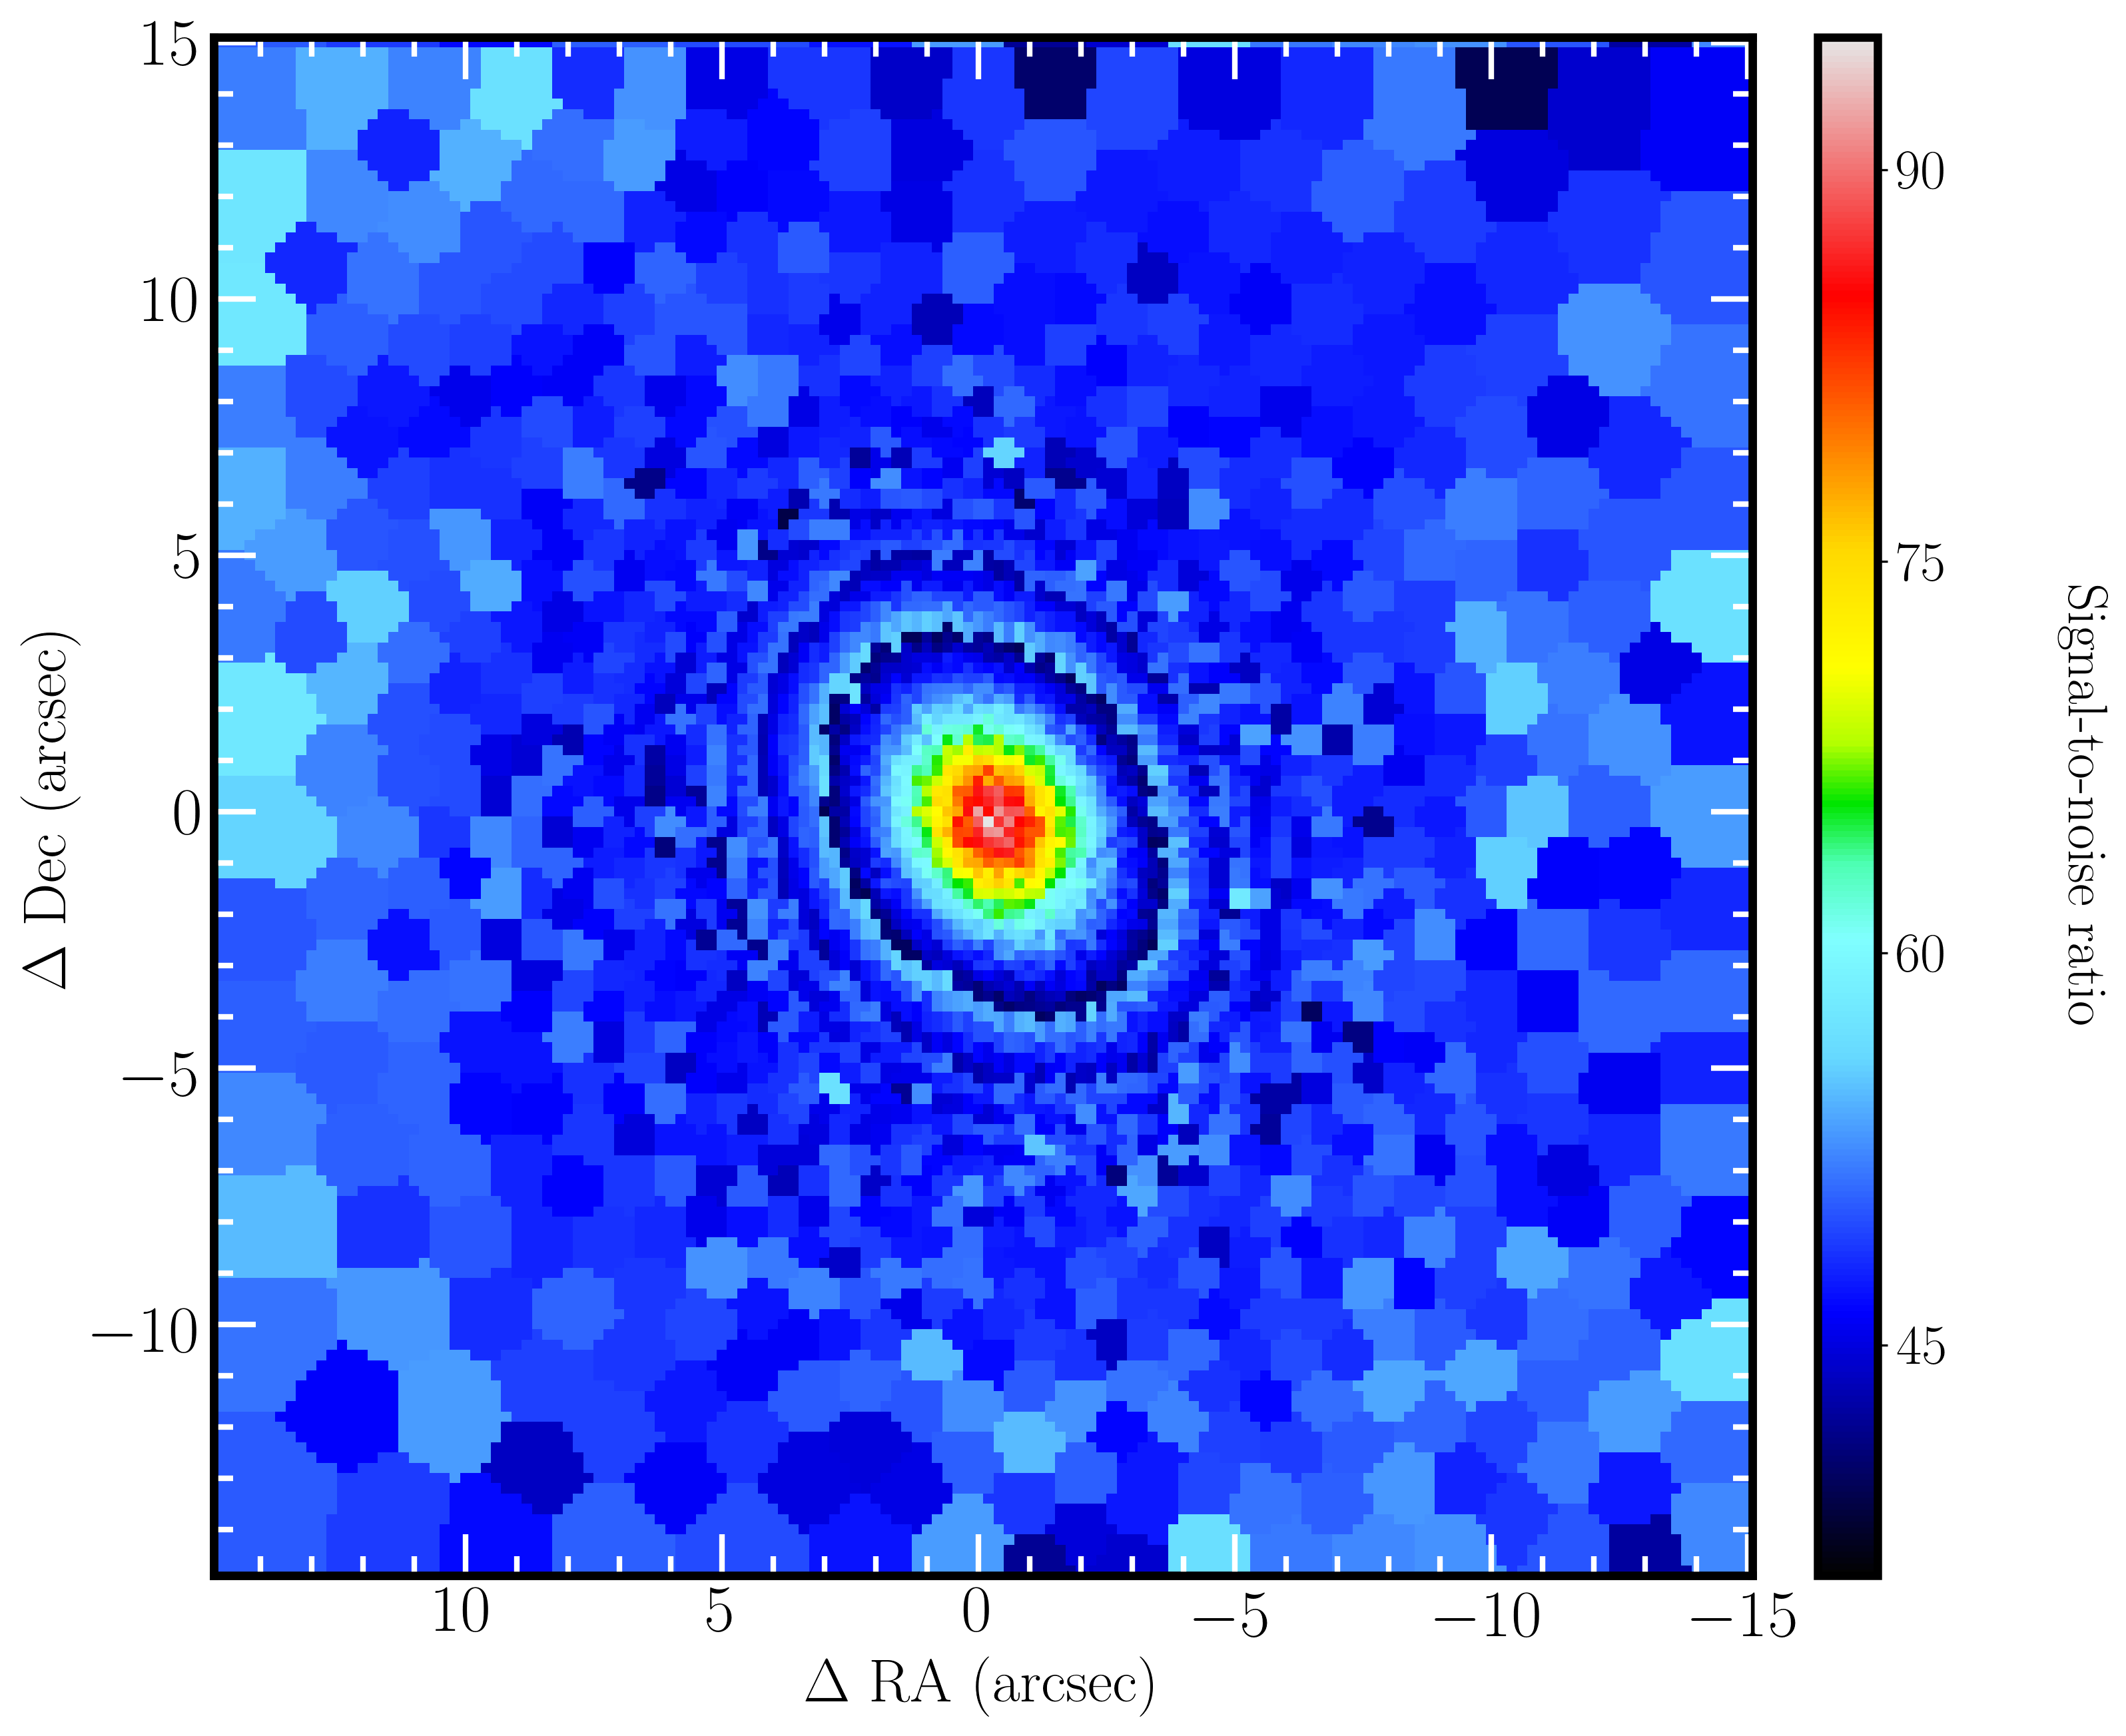
\includegraphics[width=.6\textwidth]{chapter2/egSNR.png}
			\caption[Example signal-to-noise map]{Example signal-to-noise ratio (S/N) map, from the MUSE observations of IC 1459.}
			\label{fig:egSNR}
		\end{figure}

	\subsection{Stellar Kinematics}
		\label{subsec:StellarFit}
		For our analysis, we make use of the penalized-fitting (\textsc{pPXF}) routine\footnote{\url{http://www-astro.physics.ox.ac.uk/~mxc/software/}} of \citet{Cappellari2004} and \citet{Cappellari2016a}. This routine finds the best-fitting stellar kinematics of each bin by minimizing the reduced chi-square ($\chi^2_\text{red}$) of a model spectrum built from a linear combination of empirical stellar templates, convolved with a Gaussian LOSVD (here parametrised by the mean velocity, $v$, and velocity dispersion, $\sigma$). Gaussian templates are also used to independently fit emission lines from the interstellar medium (ISM), with their own LOSVDs. Throughout our analysis, we fit all emission lines as a single component independently from the stars, and thus they have individual fluxes (except for fixed flux ratios within forbidden line doublets) but the same kinematics. \textsc{pPXF} requires an initial guess for the LOSVD of each component and we use here the redshift of the galaxy and $\sigma = 200\,\mathrm{km\,s^{-1}}$ for both components (stars and gas). Finally, Lagrange polynomials are used to make additive and/or multiplicative corrections to the continuum level of the fit. A potential sky line at 5199\,\AA\ in the Earth's frame of reference is masked in all fits.

		It was noted that for NGC 1316, the NaD absorption feature (which as generally attributed to absorption from the ISM and is thus affected by the kinematics of the ISM) was significantly effecting the quality of the stellar best-fitting spectrum. For this reason, the wavelength range of NGC 1316 spectra was limited to $<5800 \, \AA$ whilst fitting for the stellar spectra only.

		To improve the speed of our analysis, we first collapse each datacube spatially to produce a global spectrum of the galaxy, by summing across both spatial dimensions at each wavelength. The entire MILES stellar library \citep{Sanchez-Blazquez2006, Falcon-Barroso2011a} is then used to provide templates for the \textsc{pPXF} fit. We mask $600\,\mathrm{km\,s^{-1}}$--wide regions around potential emission lines (see Table \ref{tab:EmissionLine}), and use a fourth order Lagrange polynomial for an additive continuum correction. Here we use the redshift values from Simbad \citep{Wenger2000} as our initial velocity guesses. For our 14 datacubes (10 VIMOS and 4 MUSE datacubes), these fits use an average of 23 templates (with non-zero weights) out of 985. The other templates are discarded for all future analyses of a given datacube. This drastically improves the runtime of \textsc{pPXF} without affecting the quality of the fits.

		Next we implement a routine to find more optimal initial guesses of the mean velocity and velocity dispersion for each galaxy, to be used when fitting in divided bins, by means of iterative fits to the global spectrum. For each galaxy, the initial fit is set up in the same way as in the previous step, but only using the templates with non-zero weights. For each fit, the best-fitting mean velocity and velocity dispersion of the previous fit are used as the initial \textsc{pPXF} guesses, thus iteratively improving the initial guesses with each subsequent fit. The final mean velocity of a given galaxy, is used as its precise spectroscopic redshift and is given in Table \ref{tab:sample}. 

		% After the first three repetitions, the velocity was used to calculate the precise redshift of the galaxy: these are the redshift values quoted in \ref{tab:sample}. After this, small random perturbations to the iterative initial estimates are applied to ensure that the routine converges on a global minimum chi-squared, rather than a local one. 100 repetitions are run, with the mean velocities and velocity dispersions recorded and used as the initial estimates for all subsequent fits in that datacube. 

		Beyond this point, each bin is analysed independently. Each one is processed through \textsc{pPXF} using only the MILES templates with non-zero weights identified above, using the redshift and velocity dispersion estimates from the last step as initial guesses. Again, regions around potential emission lines are masked, and a fourth order polynomial additive continuum correction is used. The residuals between the best-fitting spectrum and the input spectrum are smoothed in wavelength using a weighted, moving average. This is then summed in quadrature with the noise spectrum (as propagated through the data reduction pipeline) to produce a combined `residual noise' spectrum. A Monte--Carlo (MC) estimate of the uncertainties, with 1000 repetitions is used, whereby in each iteration (after the first), random noise is added to the best-fitting model from the first run, distributed with a Gaussian profile of width equal to the residual noise. The standard deviation of the best-fitting parameters from these 1000 iterations are then adopted as the best-fitting uncertainties.

		% For accurate estimates of the uncertainties on these best-fitting values, a Monte--Carlo, with 1000 repetitions is used. In each iteration (after the first), random noise, distributed with a Gaussian profile and an amplitude comparable to the noise propagated through the data reduction pipeline, is added to the best-fitting spectrum from the first run. The standard distribution of the fitted parameters from each iteration is used as the quoted uncertainty.


	\subsection{Emission-line Kinematics}
		\label{subsec:EmissionFit}
		Deriving the distribution and kinematics of the emission lines is achieved in a manner similar to that of deriving the stellar kinematics. However, to minimize template mismatch, whereby emission lines are erroneously fitted to the edges of badly modelled and thus subtracted absorption features, we follow the method set out in \citet{Sarzi2005}. This is a three-step process, applied to each bin:
		\begin{enumerate}
			\item The region around each emission line's rest-frame wavelength is masked, and the stellar spectrum is fitted, ignoring the masked regions.
			\item The kinematics of the stellar component (i.e.\ all stellar templates) is fixed to that found in step 1. The region around the [\ion{O}{iii}] doublet is then unmasked and fitted with two (one for each doublet component) additional (and positive) Gaussians with a single free amplitude, mean velocity and velocity dispersion. The ratio of the amplitudes is fixed to 0.35.
			\item All potential emission lines are unmasked and fit with additional Gaussians, but with their kinematics fixed to that of [\ion{O}{iii}] derived in Step 2. Only the amplitudes of the Gaussians (i.e.\ the amplitude of the emission lines) therefore fit. 
		\end{enumerate}
		All the steps above are repeated with the aforementioned MC method to estimates the uncertainties, and include a tenth order multiplicative Lagrange polynomial to account for poorly modelled continuum emission. The ratio of the amplitudes of the constituent emission lines within a doublet is fixed for some forbidden lines (see Table \ref{tab:EmissionLine}).

		For each fitted emission line $i$, the ratio of the amplitude of the fitted line to the median residual noise across the line, $(A/N)_i$, is used to estimate the reliability of the detection threshold. As in \citet{Sarzi2005}, a fit to the [\ion{O}{iii}] doublet only is considered a detection if $(A/N)_{[\text{\ion{O}{iii}}]} \ge 4$. For all other lines except [\ion{N}{i}], a fit to the line is only considered a detection if [\ion{O}{iii}] is detected in the same bin and $(A/N)_i \ge 3$. For a fit to the [\ion{N}{i}] doublet, we require a detection of both [\ion{O}{iii}] and H$\beta$ and $(A/N)_{[\text{\ion{N}{i}}]} \ge 4$. The emission lines considered are listed in Table \ref{tab:EmissionLine}, along with their rest wavelengths and that of any doublet counterparts (for so-called forbidden lines). 

	 	\begin{table}
	 		\centering
	 	\begin{threeparttable}
	 		\caption{Emission lines considered in the \textsc{pPXF} fits. Every emission line given below, within the wavelength range of a given datacube was included in the analysis, thus VIMOS datacubes are fitted with H$\gamma$, H$\beta$, \brackets{\ion{O}{iii}} and \brackets{\ion{N}{i}} lines and doublets, while MUSE datacubes are fitted with H$\beta$, \brackets{\ion{O}{iii}}, \brackets{\ion{N}{i}}, \brackets{\ion{O}{i}}, \brackets{N}{ii}, H$\alpha$ and \brackets{\ion{S}{ii}} lines and doublets.}
	 		\label{tab:EmissionLine}
	 		\begin{tabular}{l c c c}
	 		\hline
	 		\hline
	 		Emission Line & Rest-frame & Doublet rest-frame & Amplitude ratio \\
	 		 & wavelength & wavelength & \\
	 		 & (\AA) & (\AA) \\
	 		\hline
	 		% \bracket{\ion{O}{ii}} 	& 3726.03 & 3728.82 & Free \\
	 		% H$\delta$ 	& 4101.76 & -- & -- \\
	 		H$\gamma$ 	& 4340.47 & -- & -- \\
	 		H$\beta$ 		& 4861.33 & -- & -- \\
	 		\bracket{\ion{O}{iii}}	& 4958.92 & 5006.84 & 0.35 \\
	 		\bracket{\ion{N}{i}} 	& 5199.36 & 5201.86 & 0.65 \\
	 		\bracket{\ion{O}{i}} 	& 6300.30 & 6363.67 & 0.33 \\
	 		\bracket{\ion{N}{ii}} 	& 6548.03 & 6583.41 & 0.34 \\
	 		H$\alpha$ 	& 6562.30 & -- & -- \\
	 		\bracket{\ion{S}{ii}} 	& 6716.47 & 6730.85 & Free \\
	 		\hline
	 		\hline
	 		\end{tabular}
	 		\begin{tablenotes}
	 		\note Col\,1: Emission line name. Col\,2: Emission line rest-frame wavelength. Col\,3: Doublet rest-frame wavelength for forbidden lines. Col\,4: The fixed ratio of the amplitudes of the lines within a doublet. `Free' indicates the amplitudes of both doublet constituents are fit independently of each other. 
	 		\end{tablenotes}
	 	\end{threeparttable}
	 	\end{table}




	 \subsection{Stellar Populations}
	 	\label{subsec:PopFit}
	 	To investigate the stellar populations of our sample galaxies we assume that a given spectrum (a global, spatially-integrated spectrum or the spectrum of a single bin) is well approximated by a single stellar population (SSP), i.e.\ that this spectrum is well represented by a collection of stars all born at the same time, in the same environment (i.e.\ with a unique combination of age, metallicity and $\alpha$-element over/under-abundance). 

	 	There are two methods to find the best-fitting SSP: full spectral fitting using synthetic spectra with different properties, and comparison of empirical or modelled line strengths to observed absorption line strengths. The former has the advantage of utilizing more information, fitting fine structure features in the spectrum and easily finding complex stellar populations. It does, however, rely on highly accurate synthetic spectra for each combination of stellar population properties considered. Also, for massive ETGs, fine spectral feature are lost because of the smoothing caused by the high velocity dispersions. The latter has the advantage of only considering the parts of the spectrum that are highly sensitive to the stellar population. It can also more easily be based on empirical observations of stars in the solar neighbourhood, and is thus less model dependent.
	 	% Interpolation between well-populated regions of the parameter space of the stellar population properties can be used to minimize the errors in sparse regions of the parameter space. 
	 	We also found that full spectral fitting almost always converged to an extreme corner of the parameter space, presumably because the model spectra are not accurate enough or our data still contains instrumental artefacts. For these reasons, we adopted the absorption line strength approach.

	 	\subsubsection{Absorption Line Strengths}
	 		\label{subsubsec:Absorption}
	 		Absorption line strength indices are defined as equivalent widths. Each index consists of 3 bandpasses: one blue and one red continuum bandpass on either side of a central bandpass containing the absorption feature of interest. A pseudo-continuum $F_\mathrm{C}(\lambda)$ is defined as the straight line between the two continuum bandpasses, assigning the median flux of each bandpass to its central wavelength. The index $I$ is then measured as the equivalent width of the spectrum $F_\mathrm{I}(\lambda)$ within the central bandpass (sampling from wavelength $\lambda_1$ to $\lambda_2$), with respect to the pseudo-continuum. For the so-called atomic indices, measured in \AA, this yields
	 		\begin{align}
	 			I_\text{\AA} \equiv \, & \int^{\lambda_2}_{\lambda_1} \! \left[1 - \frac{F_\mathrm{I}(\lambda)}{F_\mathrm{C}(\lambda)}\right] \, \mathrm{d}\lambda \, , \\
	 		\intertext{while for molecular indices, measured in magnitude, this yields}
	 			I_\text{mag} \equiv \, & -2.5 \log\left[\frac{1}{\lambda_2 - \lambda_1} \int^{\lambda_2}_{\lambda_1} \! \frac{F_\mathrm{I}(\lambda)}{F_\mathrm{C}(\lambda)} \, \mathrm{d}\lambda\right] \, .
	 		\end{align}
	 		The indices used for this project, along with their defining rest-frame bandpasses, are taken from \citet{Trager1998} and are listed in Table \ref{tab:abIndex}. All spectra are appropriately shifted to account for their systematic stellar velocity (redshift). 

		 	\begin{table}
				\centering
			\begin{threeparttable}
				\caption{Line index bandpass definitions. All absorption indices where the entirety of all bandpasses within the rest-frame wavelength range of a given datacube are measured, thus G4300, Fe4383, Ca4455, Fe4531, H$\beta$ and Fe5015 indices are measured for all VIMOS datacubes, while Mg\,b is measured for most VIMOS datacubes (the red continuum band is redshifted out of the wavelength range of NGC 612 and PKS 718-34). H$\beta$, Fe5015, Mg\,b, Fe5270, Fe5335, Fe5406, Fe5709, Fe5782, NaD, TiO1 and TiO2 are measured for all MUSE datacubes.}
				\label{tab:abIndex}
				\begin{tabular}{l c c c}
					\hline
					\hline
					Index 	& Blue continuum & Index band & Red continuum \\
					 & (\AA) & (\AA) & (\AA) \\ 
					\hline 
					G4300 	& 4266.375\,--\,4282.625 & 4281.375\,--\,4316.375 & 4318.875\,--\,4335.125 \\
					Fe4383 	& 4359.125\,--\,4370.375 & 4369.125\,--\,4420.375 & 4442.875\,--\,4455.375 \\
					Ca4455 	& 4445.875\,--\,4454.625 & 4452.125\,--\,4474.625 & 4477.125\,--\,4492.125 \\
					Fe4531 	& 4504.250\,--\,4514.250 & 4514.250\,--\,4559.250 & 4560.500\,--\,4579.250 \\
					H$\beta$ & 4827.875\,--\,4847.875 & 4847.875\,--\,4876.625 & 4876.625\,--\,4891.625 \\
					Fe5015 	& 4946.500\,--\,4977.750 & 4977.750\,--\,5054.000 & 5054.000\,--\,5065.250 \\
					Mg\,b 	& 5142.625\,--\,5161.375 & 5160.125\,--\,5192.625 & 5191.375\,--\,5206.375 \\
					Fe5270 	& 5233.150\,--\,5248.150 & 5245.650\,--\,5285.650 & 5285.650\,--\,5318.150 \\
					Fe5335 	& 5304.625\,--\,5315.875 & 5312.125\,--\,5352.125 & 5353.375\,--\,5363.375 \\
					Fe5406 	& 5376.250\,--\,5387.500 & 5387.500\,--\,5415.000 & 5415.000\,--\,5425.000 \\
					Fe5709 	& 5672.875\,--\,5696.625 & 5696.625\,--\,5720.375 & 5722.875\,--\,5736.625 \\
					Fe5782 	& 5765.375\,--\,5775.375 & 5776.625\,--\,5796.625 & 5797.875\,--\,5811.625 \\
					NaD 	& 5860.625\,--\,5875.625 & 5876.875\,--\,5909.375 & 5922.125\,--\,5948.125 \\
					TiO1 	& 5816.625\,--\,5849.125 & 5936.625\,--\,5994.125 & 6038.625\,--\,6103.625 \\
					TiO2 	& 6066.625\,--\,6141.625 & 6189.625\,--\,6272.125 & 6372.625\,--\,6415.125 \\
					\hline
					\hline
				\end{tabular}
				\begin{tablenotes}
				\footnotesize
				\note All index definitions are from \citet{Trager1998}. All bandpasses are defined in the rest frame and as such all spectra must be appropriately shifted to account for the redshift of the stars. 
				\end{tablenotes}
			\end{threeparttable}
			\end{table}

			Much of the literature provides absorption line strength measurements in the Lick/Cassegrain Image Dissector Scanner spectrograph system (hereafter Lick/IDS system; \citealt{Faber1985, Worthey1994}), but this has several disadvantages. Firstly, the Lick/IDS system is based on non-flux-calibrated spectra from the IDS spectrograph on the Shane telescope (Lick Observatory), that has a relatively low and wavelength-dependent spectral resolution. When using the Lick/IDS system with other instruments, it is thus necessary to calibrate the observations by performing empirical corrections aiming to compensate for the uncalibrated continua of the Lick/IDS data. This requires observations of standard stars using the same instrumental set-up as the main observations. Since this was not requested as part of the VIMOS observing strategy and standard star observations are thus unavailable, we are unable to transform our measurements to the Lick/IDS system. An additional/new proposal is not possible either, as VIMOS has been substantially upgraded in the intervening time. Given the low spectral resolution and poor data quality on which the Lick/IDS system is based, we believe in any case that the community should be making a concerted effort to use alternative systems. We therefore choose to use the line index system (LIS) of \citet{Vazdekis2010}. LIS is based on flux-calibrated measurements at several spectral resolutions (5.0, 8.4 and 14.0\,\AA\ FWHM). \citet{Vazdekis2010} also provide empirical cubic functions to transform Lick/IDS literature measurements to LIS\footnote{\url{http://www.iac.es/proyecto/miles/pages/line-index-system-lis/transformations.php}}.

			Because of the models we use for stellar population fitting (see Section \ref{subsubsec:StellarPop}), we actually measure the absorption line indices at a slightly degraded spectral resolution of 2.5\,\AA. For comparisons to the literature (Section \ref{subsec:absorption}), we also measure the absorption line indices at 8.4\,\AA\ resolution. 

			Since our aim is to find the best-fitting stellar population model, it is important to first remove the contribution of the ISM to the spectra. This involves fitting for and subtracting the emission lines detected (as described in Section \ref{subsec:EmissionFit}). 

			We must also correct for the effect of the different velocity dispersions of the stellar populations, that varyingly spread absorption features such that differing fractions of the absorption are outside of the central bandpasses. To do this, we simply create a best-fitting spectrum (as in the previous step) that is not convolved with the best-fitting LOSVD. Note that for NGC 1316, for indices with a wavelength longer than 5800\,\AA\, we use the extrapolated best-fitting pPXF fit. A given index, $I$, is then measured for both this `unconvolved' spectrum ($I^\text{unc}$) and the convolved best-fitting spectrum ($I^\text{conv}$), and the ratio of these two indices is used as a multiplicative correction factor for the index measured ($I^\text{obs}$), such that the corrected index ($I^\text{corr}$) is given by
			\begin{equation}
				I^\text{corr} \equiv \frac{I^\text{unc}}{I^\text{conv}} I^\text{obs} \, .
				\label{eq:absCorrection}
			\end{equation}
			These corrected indices are those reported and discussed in the sections below and in Section \ref{subsec:absorption}.


		\subsubsection{Stellar Population Models}
			\label{subsubsec:StellarPop}
			The final step of the data analysis pipeline is to find the best-fitting SSP model of a given spectrum. Sets of SSP models consist of a grid of models characterised by stellar properties such as age ($t$), metallicity ([Fe/H]) and alpha-element enhancement ([$\alpha$/Fe]). Here, we first provide a generic overview of the process of generating synthetic stellar population models, and then detail the specific of the models adopted. 

			Synthetic SSPs are created using the following components:
			\begin{itemize}
				\item the paths of stars of a given mass and metallicity as they travel across the Hertzsprung--Russell diagram (HRD) by ageing. These are known as stellar evolutionary tracks and are generally empirical.
				\item the function $\Phi(M)$, representing the number of stars formed $N(M)$ per mass interval $\mathrm{d}M$, i.e.\ $\Phi(M) \equiv \frac{\mathrm{d}N(M)}{\mathrm{d}M}$. This is the initial mass function (IMF).
				\item an empirical library of stellar spectra, to be able to assign a spectrum to each position on the HRD. 
			\end{itemize}
			The desired output of expected line strengths for a three-dimensional grid of varying age, metallicity and $\alpha$-enhancement can be computed in one of two ways: (i) by producing full synthetic spectra from the stellar evolution models sampled very finely as a function of the tree stellar parameters of interest or (ii) by finding a `fitting function' for each index, that analytically relates the index measured from an empirical library to the three stellar parameters of interest. The former is dependent on a good understanding of the physics of stellar atmospheres and is known to suffer from incomplete line lists and continuum uncertainties \citep{Thomas2004}. This would have been the appropriate method for producing synthetic spectra for full spectral fitting had we chosen that method for investigating the stellar populations of our sample galaxies (see Section \ref{subsec:PopFit}). The latter, and more popular, method allows for interpolation between well-populated regions of stellar parameter space in order to increase the accuracy of the models in stellar parameter space that are only sparsely sampled by an empirical stellar library \citep{Thomas2010}. 

			\begin{figure}
				\centering
				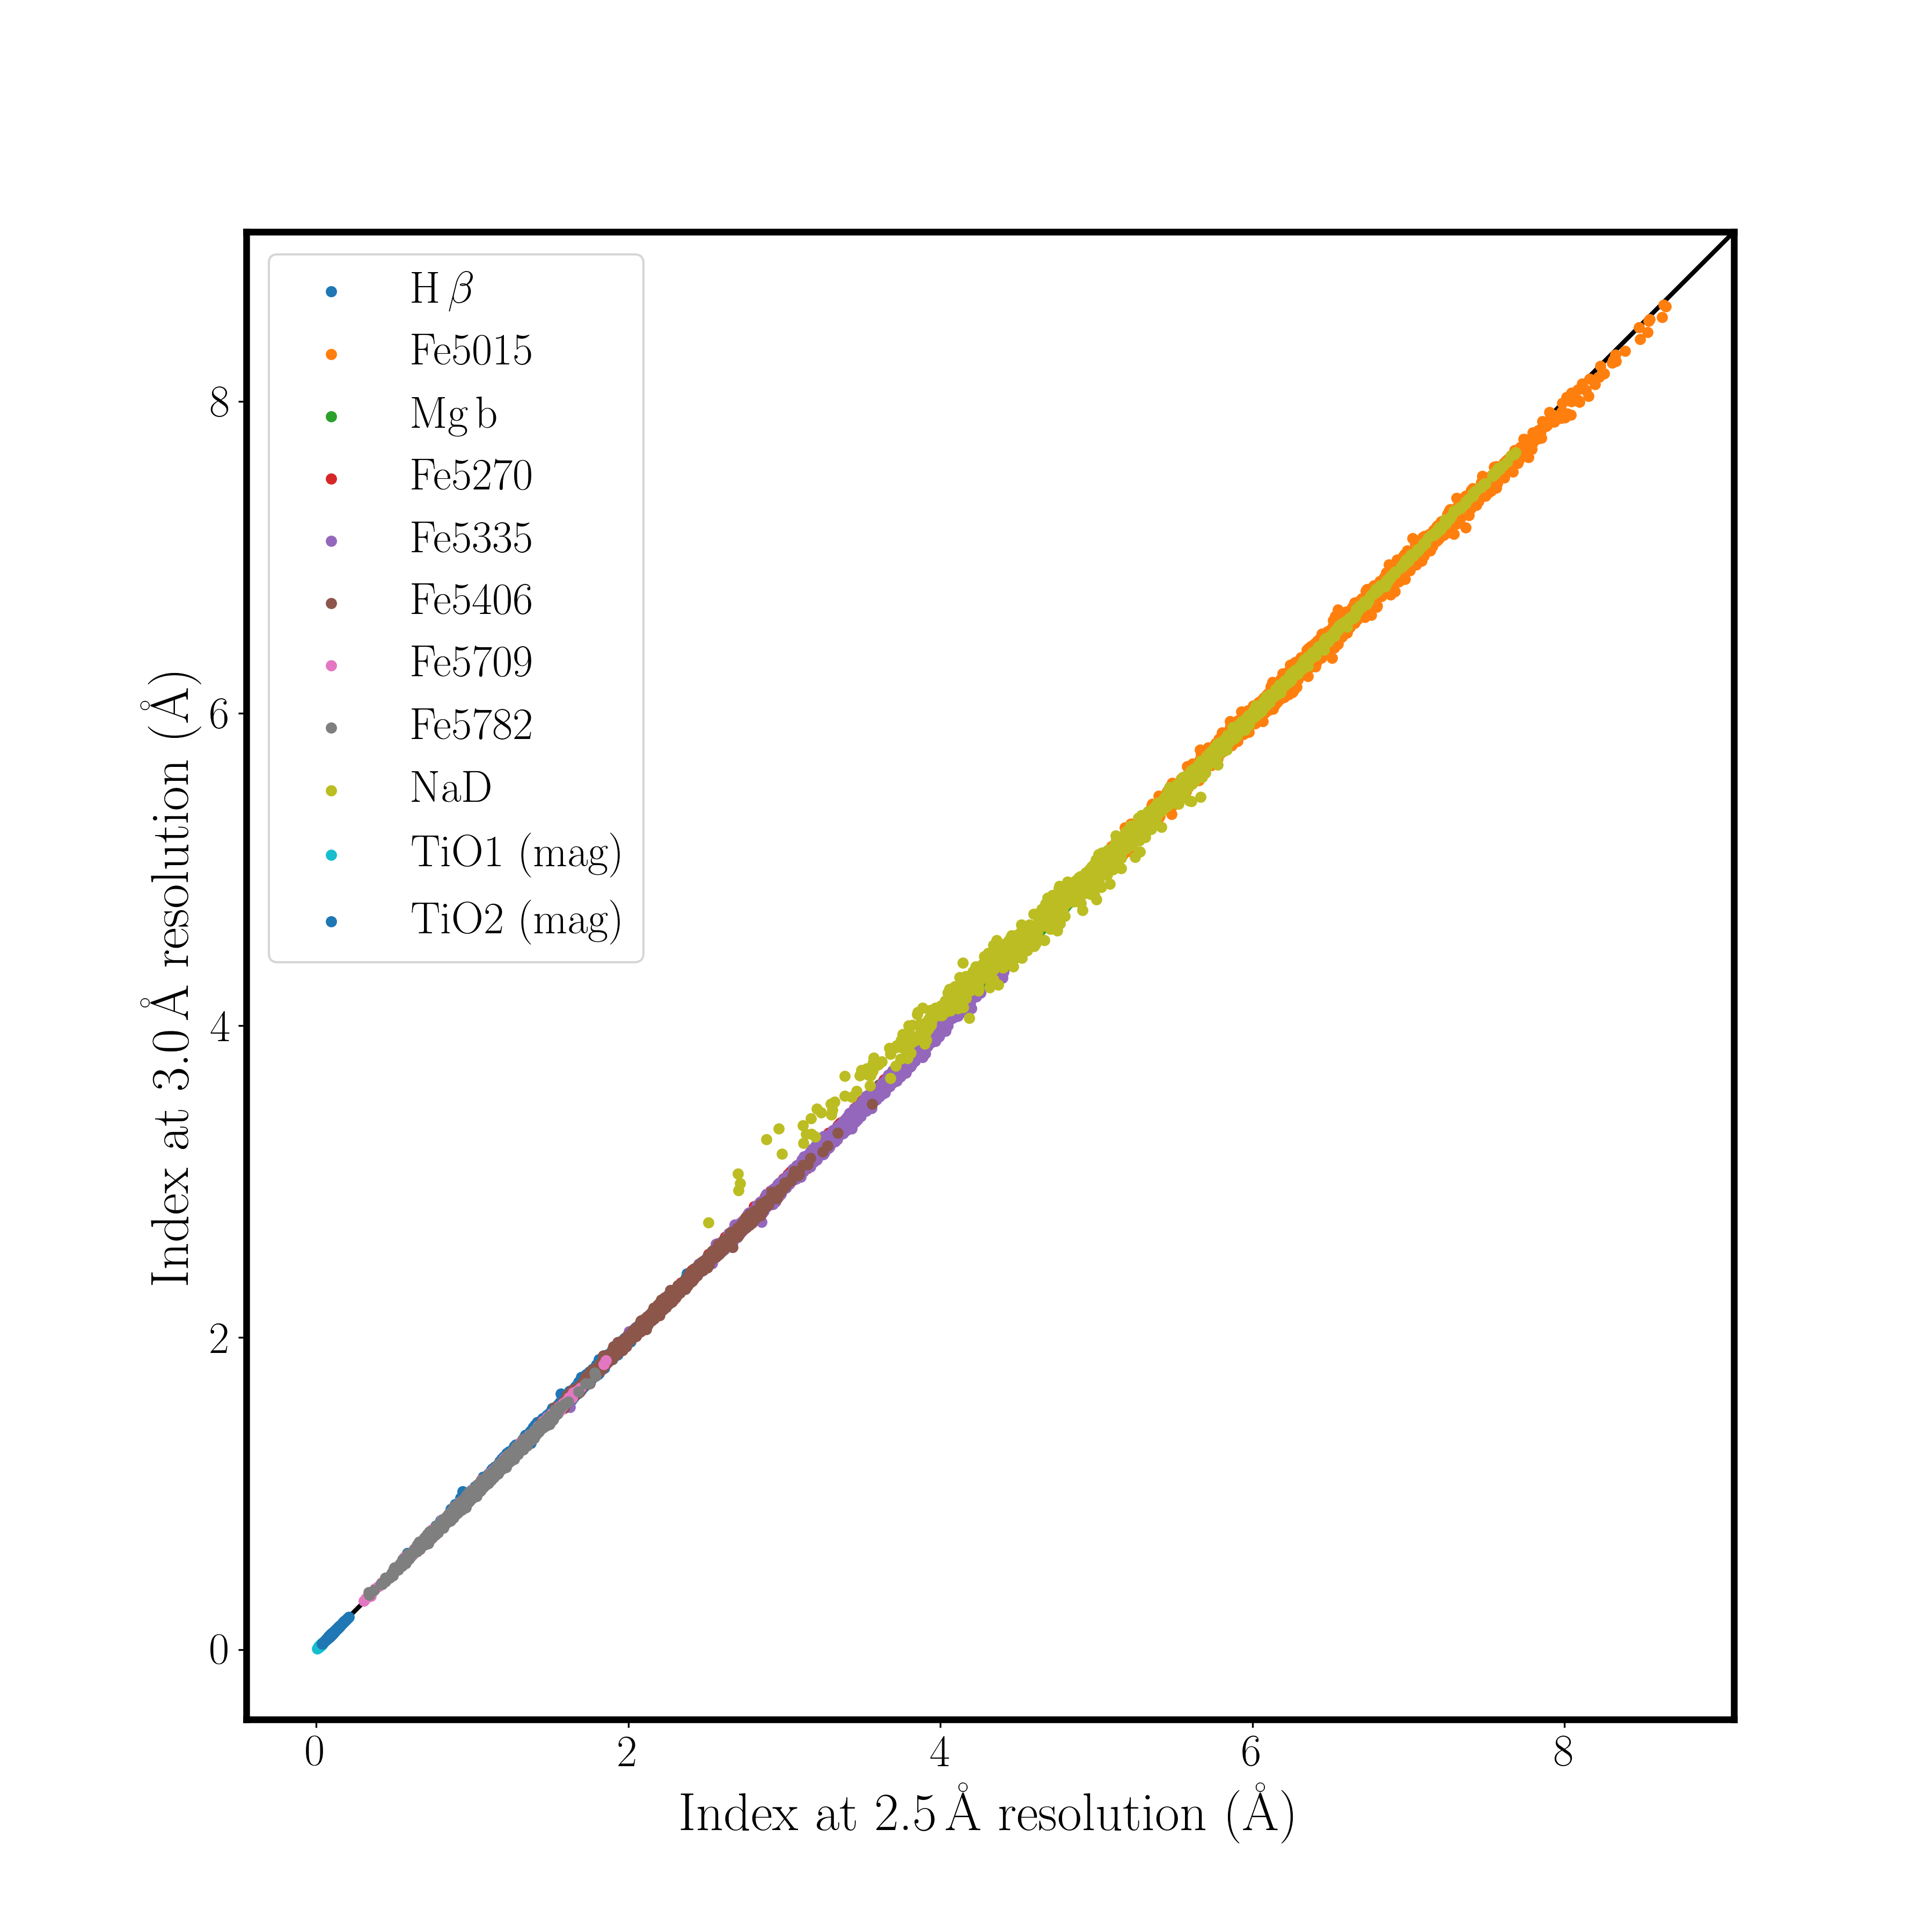
\includegraphics[width=.7\textwidth]{chapter2/compare_resolutions.png}
				\caption[Resolution effects on absorption line index strengths]{Resolution effect on absorption line strength measurements. Absorption line strength indices at 2.5\AA\ and 3.0\AA\ spectral resolution are compared, showing that the effect of a slightly lower spectral resolution is negligible. The dotted lines mark a difference of $\pm1$\% between the measurements at each resolution.}
				\label{fig:res}
			\end{figure}

			ETGs often have very different fractional abundances of the various metals than those of the nearby stars that we are able to observe (all of which have near solar abundances). As such, the empirical stellar libraries used to calibrate the models fall short of the required coverage of parameter space. Most methods somehow attempt to extrapolate their results to non-solar abundances, and in a similar way to the fitting functions described above, `index response functions' can be constructed. These attempt to calibrate the effects of the varying abundances of individual elements, and comparison must then be made to completely theoretical spectra.

			Here we use the SSP models of \citeauthor{Thomas2010} (\citeyear{Thomas2010}; hereafter TMJ), as they are based on flux-calibrated spectra and therefore do not require calibration to the Lick/IDS system. These models assume a \citet{Salpeter1955} IMF ($\Phi(M) \propto M^{-2.35}$) and are based on the evolutionary population synthesis code of \citet{Maraston1998}. The models use the stellar evolutionary tracks of \citet{Cassisi1997} for metallicities $[Z/H] < -0.33$ and of \citet{Girardi2000} for $[Z/H] \ge -0.33$, the MILES stellar spectral library of \citet{Sanchez-Blazquez2006a} and \citet{Falcon-Barroso2011a}, the fitting functions of \citet{Johansson2010} and the index response functions of \citet{Korn2005}. The MILES library and thus the models have spectral resolution of 2.5\,\AA. This is better then the resolution of the reduced VIMOS data (3\,\AA), but we show in Fig.\,\ref{fig:res} that this has a negligible effect. Indeed, comparing the absorption line strengths measured at 2.5\,\AA\ and 3\,\AA\ for the MUSE datasets shows that the worst affected index is Fe5782 with a mean difference of only 1\% between the indices measured at 3\,\AA\ and 2.5\,\AA\ resolution. All other indices show a difference of only a few tenths of a percent. 

			The response functions of \citet{Korn2005} extend the work of \citet{Tripicco1995}, who investigated the response functions of the original 21 Lick indices when the individual element abundance fractions are varied for a 5 Gyr old SSP at solar metallicity. The new functions include varying metallicities as well as individual element fractions, and are calculated for all 25 Lick indices. The effect of age on these response functions was tested by computing them for 1 Gyr models and comparing them to the 5 Gyr models of \citet{Tripicco1995}. \citet{Korn2005} found a 1\% difference for two indices (G4300 and Fe4383) and significantly smaller differences for all other indices, thus concluding that age does not significantly affect the response functions.

			Finally, individual element abundances are combined to calculate the alpha-element enhancement parameter [$\alpha$/Fe]. This is done following \citet{Trager2000}, who grouped the elements into three categories: 
			\begin{itemize}
				\item enhanced elements, including C, N, O, Na, Mg, Si, Ca and Ti (i.e.\ $\alpha$ and light elements); 
				\item depressed elements, including Cr and Fe (i.e.\ iron peak elements); and
				\item fixed elements (all other elements). 
			\end{itemize}
			The fixed-element group elements are held at solar abundances, while the enhanced-(depressed-)element group elements are scaled up (down) by the same factor. 

			The TMJ models return absorption line strength indices for a 3 dimensional grid ($t$, $[Z/H]$, [$\alpha$/Fe]) with $t$ = 0.1, 0.2, 0.4, 0.6, 0.8, 1, 2, 3, 4, 5, 6, 7, 8, 9, 10, 11, 12, 13, 14 and 15 Gyr; $[Z/H]$ = -2.25, -1.35, -0.33, 0.0, 0.35 and 0.67; and [$\alpha$/Fe] = -0.3, 0.0, 0.3 and 0.5.

			TMJ showed that their models produce good fits to globular cluster measurements of \citet{Puzia2002} and \citet{Schiavon2005} and the galaxy measurements of the SAURON team by \citet{Kuntschner2010}. \citet{Conroy2010} suggest that the stellar evolutionary tracks of \citet{Girardi2000} used for the high-metallicity models do not fit the globular clusters well, but TMJ point out that this can be explained by an anomaly in the Balmer lines that is not present in the SAURON data analysis. TMJ therefore suggest that this is an issue with the globular cluster measurements themselves. 

			% Following the method of \citet{McDermid2006}, we first linearly interpolate the TMJ models to a three-dimensional grid with sides of length 40 in age, metallicity and $\alpha$-enhancement. The metallicity and $\alpha$-enhancement axes are linearly sampled, while the age axis is logarithmically sampled. 

			Markov chain Monte--Carlo (MCMC) fitting is useful as it allows for the efficient exploration of parameter space by avoiding regions with low probabilities (high $\chi^2_\text{red}$). A large number of `walkers' are placed at an initial position (the hypothesis). In each iteration, each walker moves a random distance in a random direction. For a given walker, if the probability is higher at its new location it accepts the move, otherwise it is rejected and the walker remains in its initial position. In this thesis we choose to use \textsc{emcee}, a \textsc{python} MCMC fitting package \citep{Foreman-Mackey2013}. \textsc{emcee} is an ensemble MCMC sampler, meaning that the steps taken by each walker are influenced by the position of all the other walkers. This allows for a quicker convergence on the most-likely result. After first interpolating the 3-dimensional grid of TMJ SSP models using \textsc{LinearNDInterpolator} (a \textsc{python} package provided in \textsc{scipy}; \citealt{Barber1996}), we use the MCMC method to find the most-likely SSP model, by comparing the absorption line strength indices measured (with the method described above in Section \ref{subsubsec:Absorption}) to those of the interpolated grid models. \textsc{emcee} is an affine-invariant ensemble MCMC sampler meaning that we can take the standard deviation of the positions of the walkers in the MCMC code as the uncertainty on the most-likely stellar population.

			In Section \ref{sec:pop} we will use the results from this pipeline to compare the absorption line strength indices and the stellar populations of our Southern Sample radio galaxies to those of radio-quiet ETGs.

\chapter{MUSE data}
	\label{cha:MUSE}

\chapter{Stellar Kinematics and Populations}
	\label{cha:stellar}
% More preface here
With the advent of integral-field spectroscopy (IFS), we can now observe the spatially-resolved properties of a galaxy without relying on extrapolations of or multiple observations with slits. Surveys such as the Spectrographic Areal Unit for Research on Optical Nebulae (SAURON; \citealt{deZeeuw2002}) and Atlas$^\text{3D}$ \citep{Cappellari2011} have demonstrated that systematic IFS surveys provide a wealth of information about the structure of nearby galaxies. This chapter focuses on the resolved stellar properties of our sample of radio galaxies. In this we aim to demonstrate that our radio selected sample is no different in the $V$-band than optically-selected early-type galaxies ETGs from the MASSIVE (not an acronym; \citealt{Ma2014}) and Atlas$^\text{3D}$ samples. We achieve this by showing that they are consistent with the defining characteristics of ETGs that are accessible to $V$-band IFS data. These characteristics are (with relevant section is shown in parentheses): regular/non-regular rotator classification scheme, qualitative kinematic classes (see Fig.\,\ref{fig:EgSubstructure}; Section \ref{subsec:maps}), fast/slow rotator classifications (\ref{subsec:FSRot}), radially resolved specific angular momentum profiles (with $\lambda_R$; \ref{subsec:ResolvedLambda_R}), absorption line strengths(\ref{subsec:absorption}), Mg--$\sigma$ relation (\ref{subsubssec:Mgsigma}), stellar populations (\ref{subsec:ssp}) and their gradients (\ref{subsubsec:popGrad}) and the kinematically-decoupled core (KDC) age--size relation(\ref{subsec:popKDC}). 
% ^^^^^^^^^^^^^^^ check section references above are correct ^^^^^^^^^^^^^^^

The chapter is structured as follows: firstly we present the kinematic maps for the stellar component of each galaxy (section \ref{sec:stellarKin}) and the distribution of the sample on the $\lambda_\mathrm{R_e}$--ellipticity diagram. Then, in section \ref{sec:pop}, we investigate the stellar populations of each galaxy using the measured absorption line strengths. Finally, in Section \ref{sec:stellarDiscussion} we discuss these observation.


\section{Kinematics}
	\label{sec:stellarKin}

	\subsection{Maps}
		\label{subsec:maps}
		Using the methods described in Chapter \ref{cha:Data} to reduce (see Sections \ref{subsec:VIMOSreduction} and \ref{subsec:MUSEreduction}), spatially bin (Section \ref{subsec:Binning}) and fit the stellar line-of-sight velocity distributions (LOSVDs; here parametrised by the mean velocity, $v$ and velocity dispersion, $\sigma$, only; Section \ref{subsec:StellarFit}), we produce stellar kinematic maps. These kinematic maps are shown in Figs.\,\ref{fig:VIMOS_stellar} and \ref{fig:MUSE_stellar} with their associated uncertainties for the VIMOS and MUSE datacubes, respectively. 

		As part of this project, radio continuum maps have been produced by Robert Laing (private communication) by re-reducing archival data from the Very Large Array (VLA) in a variety of bands. We also use the VLA image from \citet{Lanz2010} for NGC 1316. These images have a variety of resolutions and spatial scales: we choose the image that closest matches our VIMOS and MUSE observations and overlay this on all maps (except those showing uncertainties) in green contours. Additionally, this project has also secured observations of the Southern Sample (except NGC 1316 and NGC 1399 for technique reasons) from the Atacama Large Millimeter/sub-millimeter Array (ALMA). \ce{^{12}CO(2-1)} flux maps have been produced by Ruffa et al.\ (in prep.). These are shown in cyan contours on all maps (except those showing uncertainties). 
% Is the radio still in green contours? 



		\begin{figure}
			\centering
			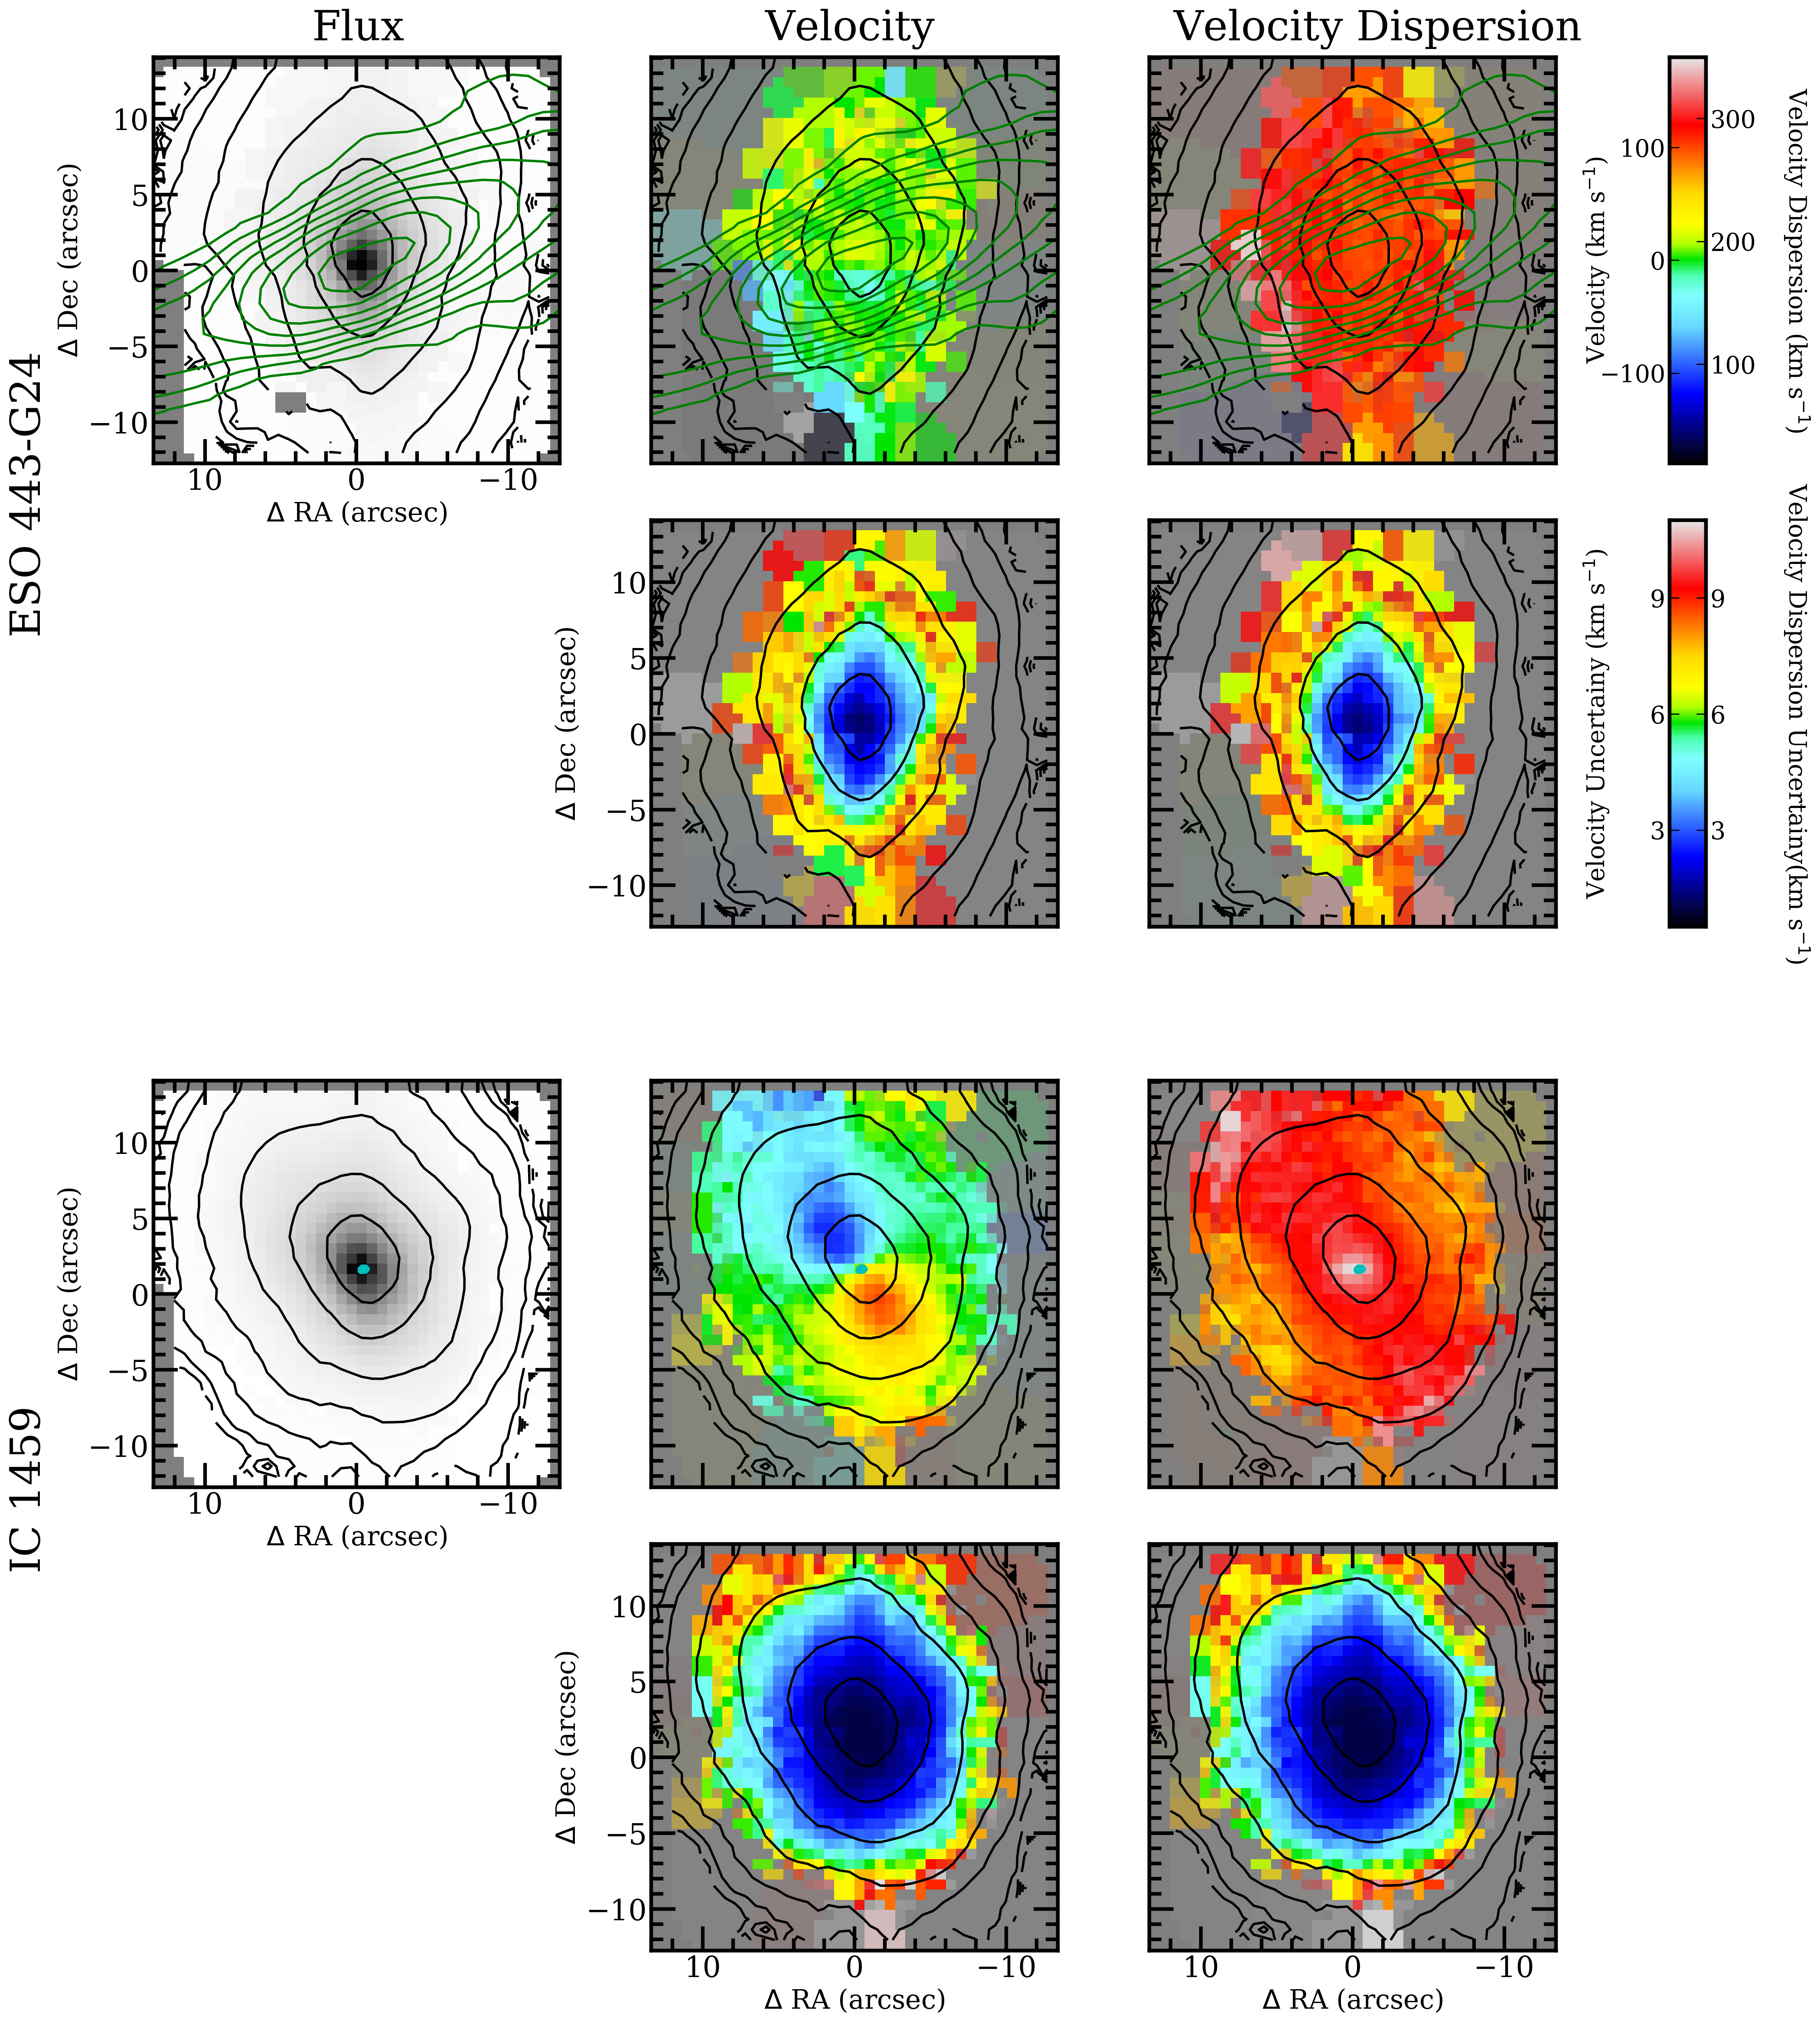
\includegraphics[height=0.62\textheight]{chapter4/vimos/kin1.png}
			\caption[VIMOS stellar kinematic maps]{VIMOS stellar kinematic maps. Left to right: flux (image), mean velocity and velocity dispersion. Top to bottom: ESO 443-G24 and IC 1459. Alternate rows show a given parameter its associated uncertainty. Flux contours (isophotes) are shown in black, \ce{^{12}CO(2-1)} contours from ALMA in cyan and radio continuum contours from VLA in green. The radio band displayed depends on the data available in the archive and which images had a similar resolution and scales. Limits on the colour scale are: mean velocity maps -180 to 180\,$\mathrm{km \, s^{-1}}$, mean velocity uncertainty 1 to 11\,$\mathrm{km \, s^{-1}}$, velocity dispersion 35 to 350\,$\mathrm{km \, s^{-1}}$ and velocity dispersion uncertainty 1 to 11\,$\mathrm{km \, s^{-1}}$.} 
			\label{fig:VIMOS_stellar}
		\end{figure}
		\begin{figure}
			\centering
			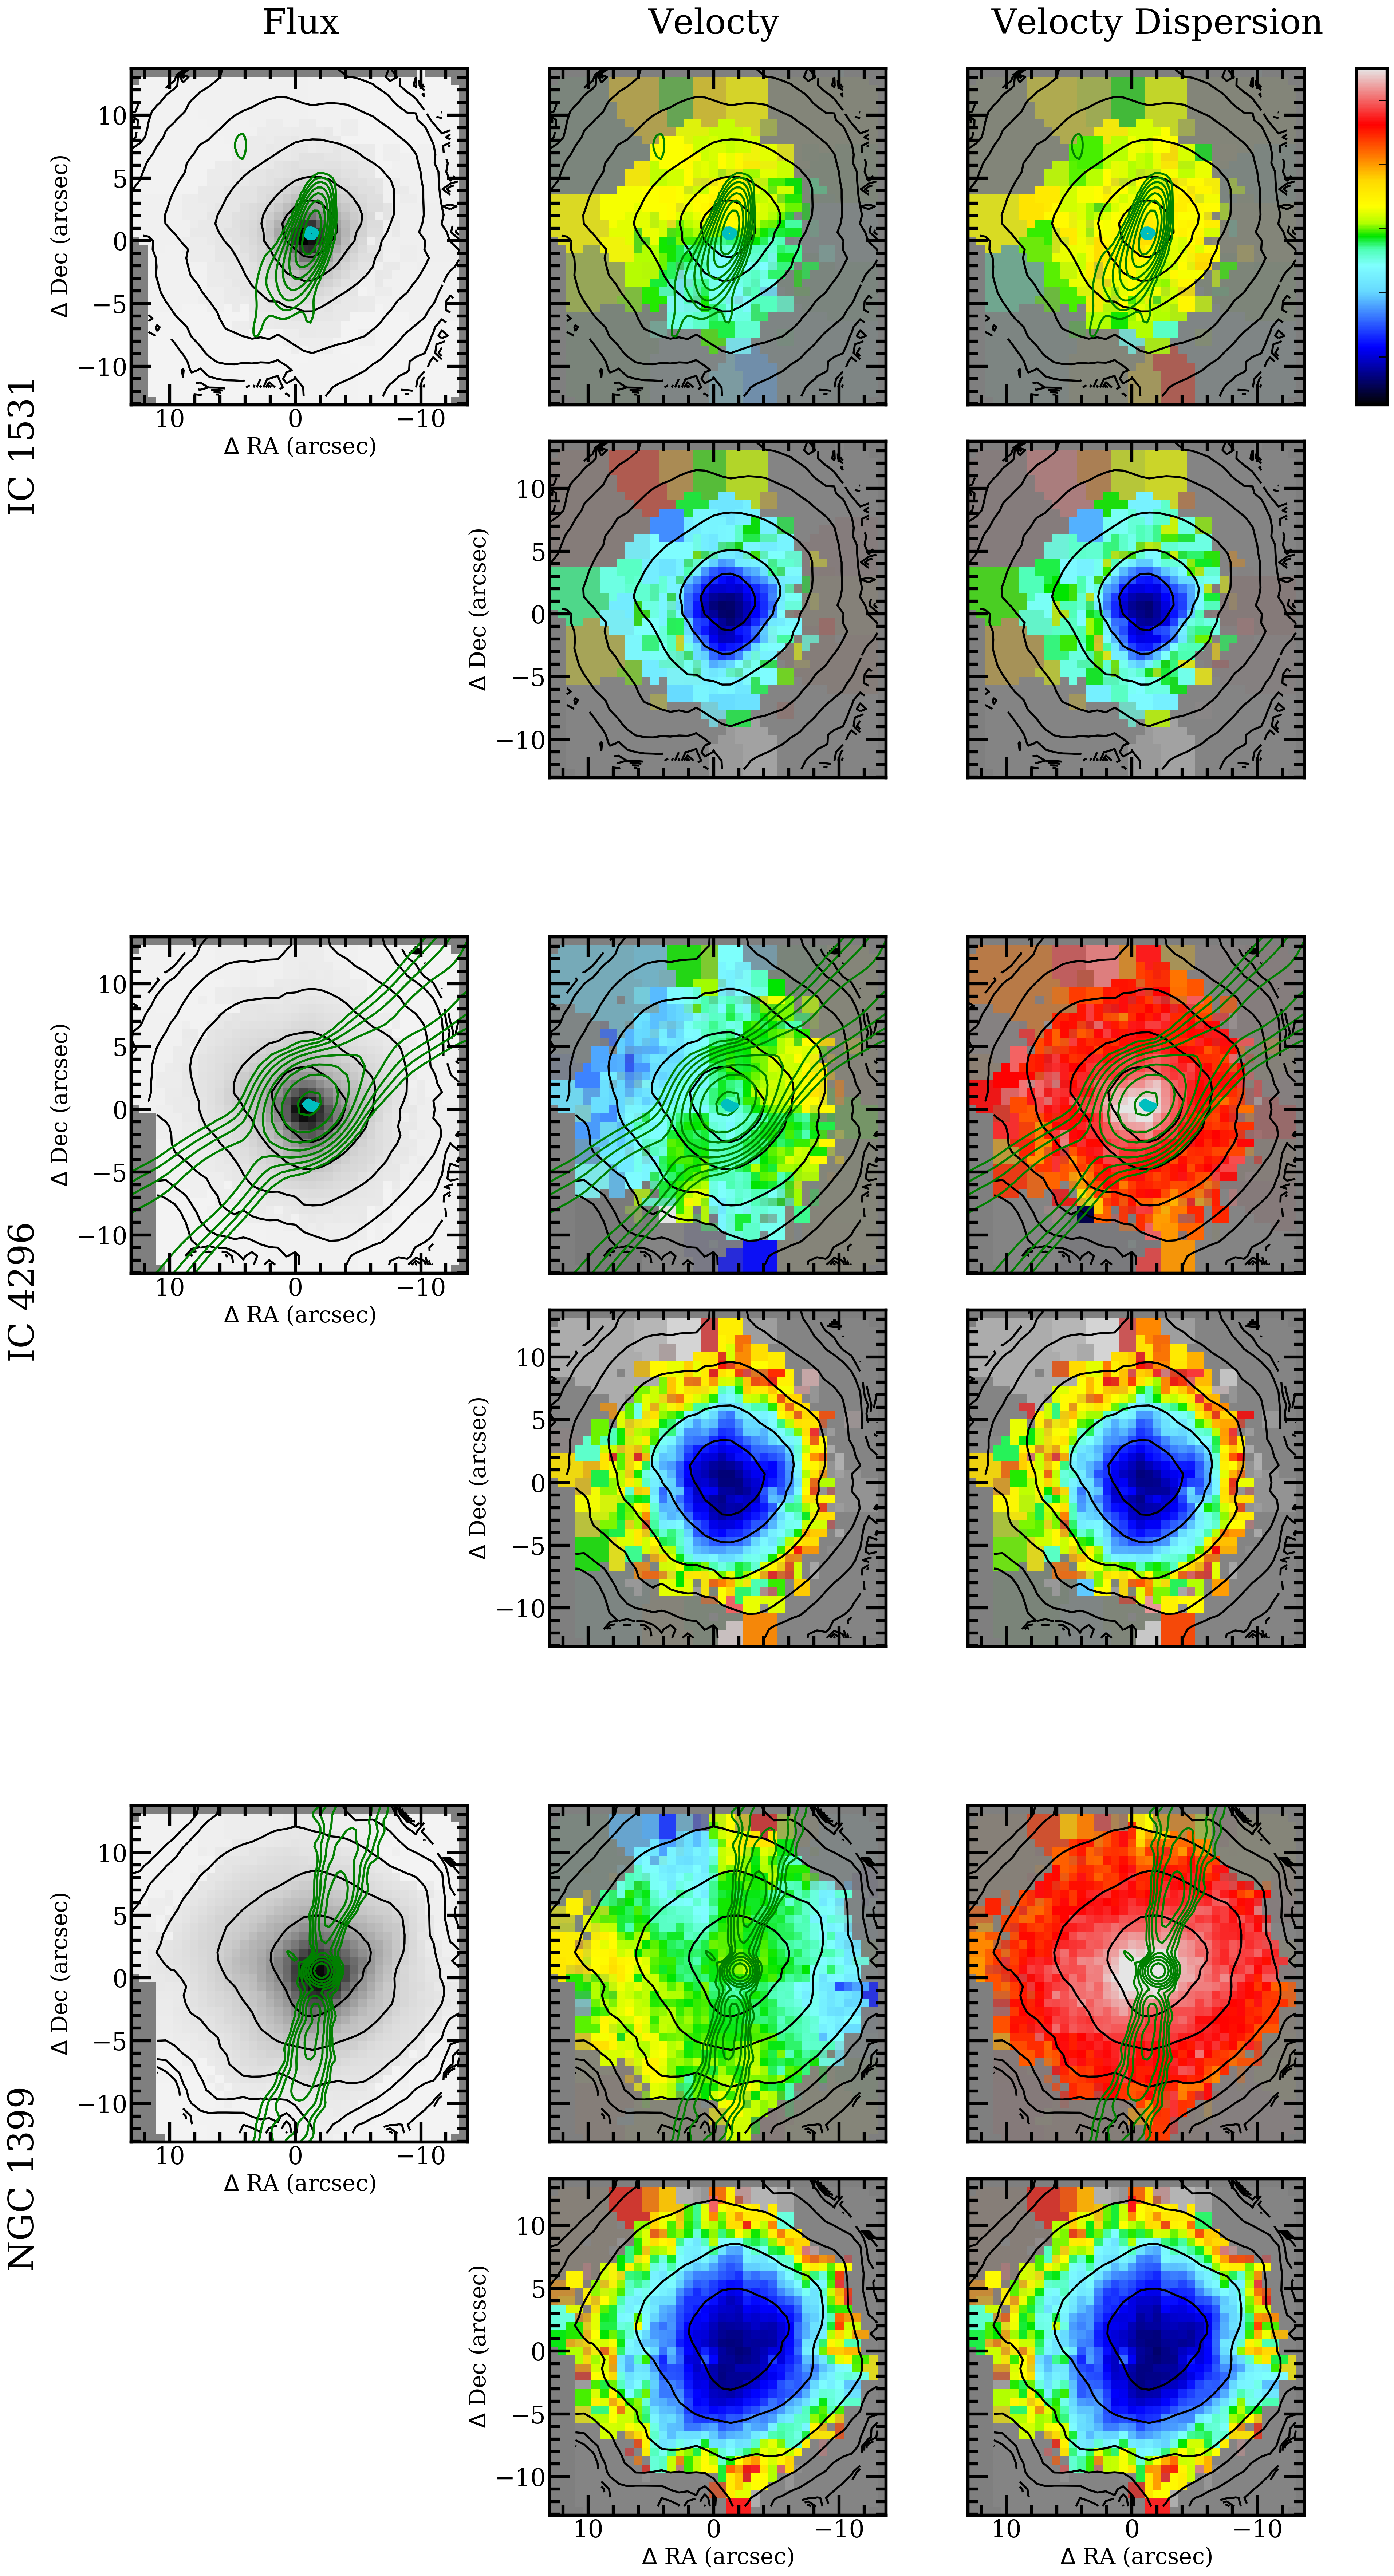
\includegraphics[height=0.94\textheight]{chapter4/vimos/kin2.png}
			\contcaption{\textit{Continued.}}
		\end{figure}
		\begin{figure}
			\centering
			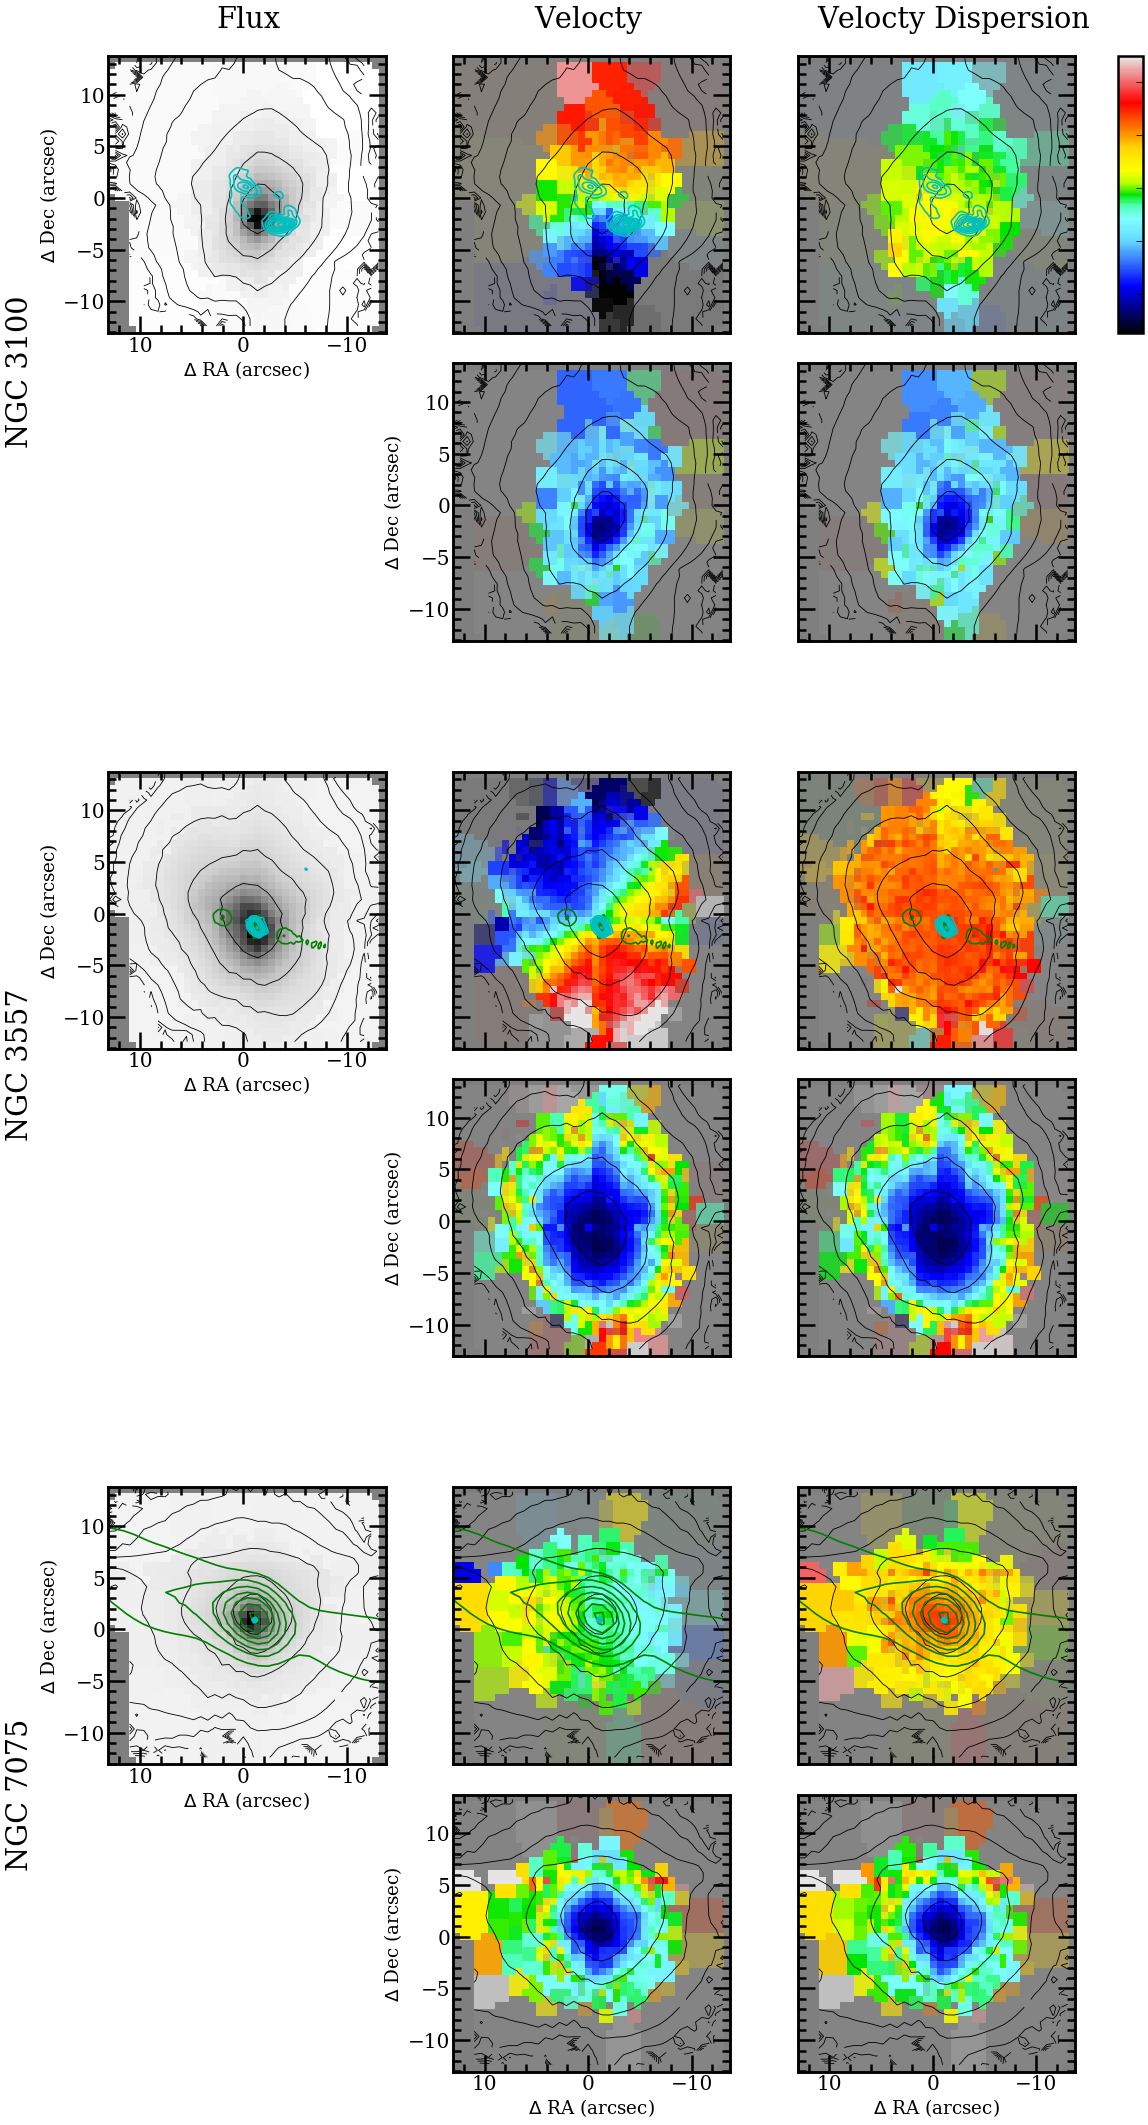
\includegraphics[height=0.94\textheight]{chapter4/vimos/kin3.png}
			\contcaption{\textit{Continued.}}
		\end{figure}
		\begin{figure}
			\centering
			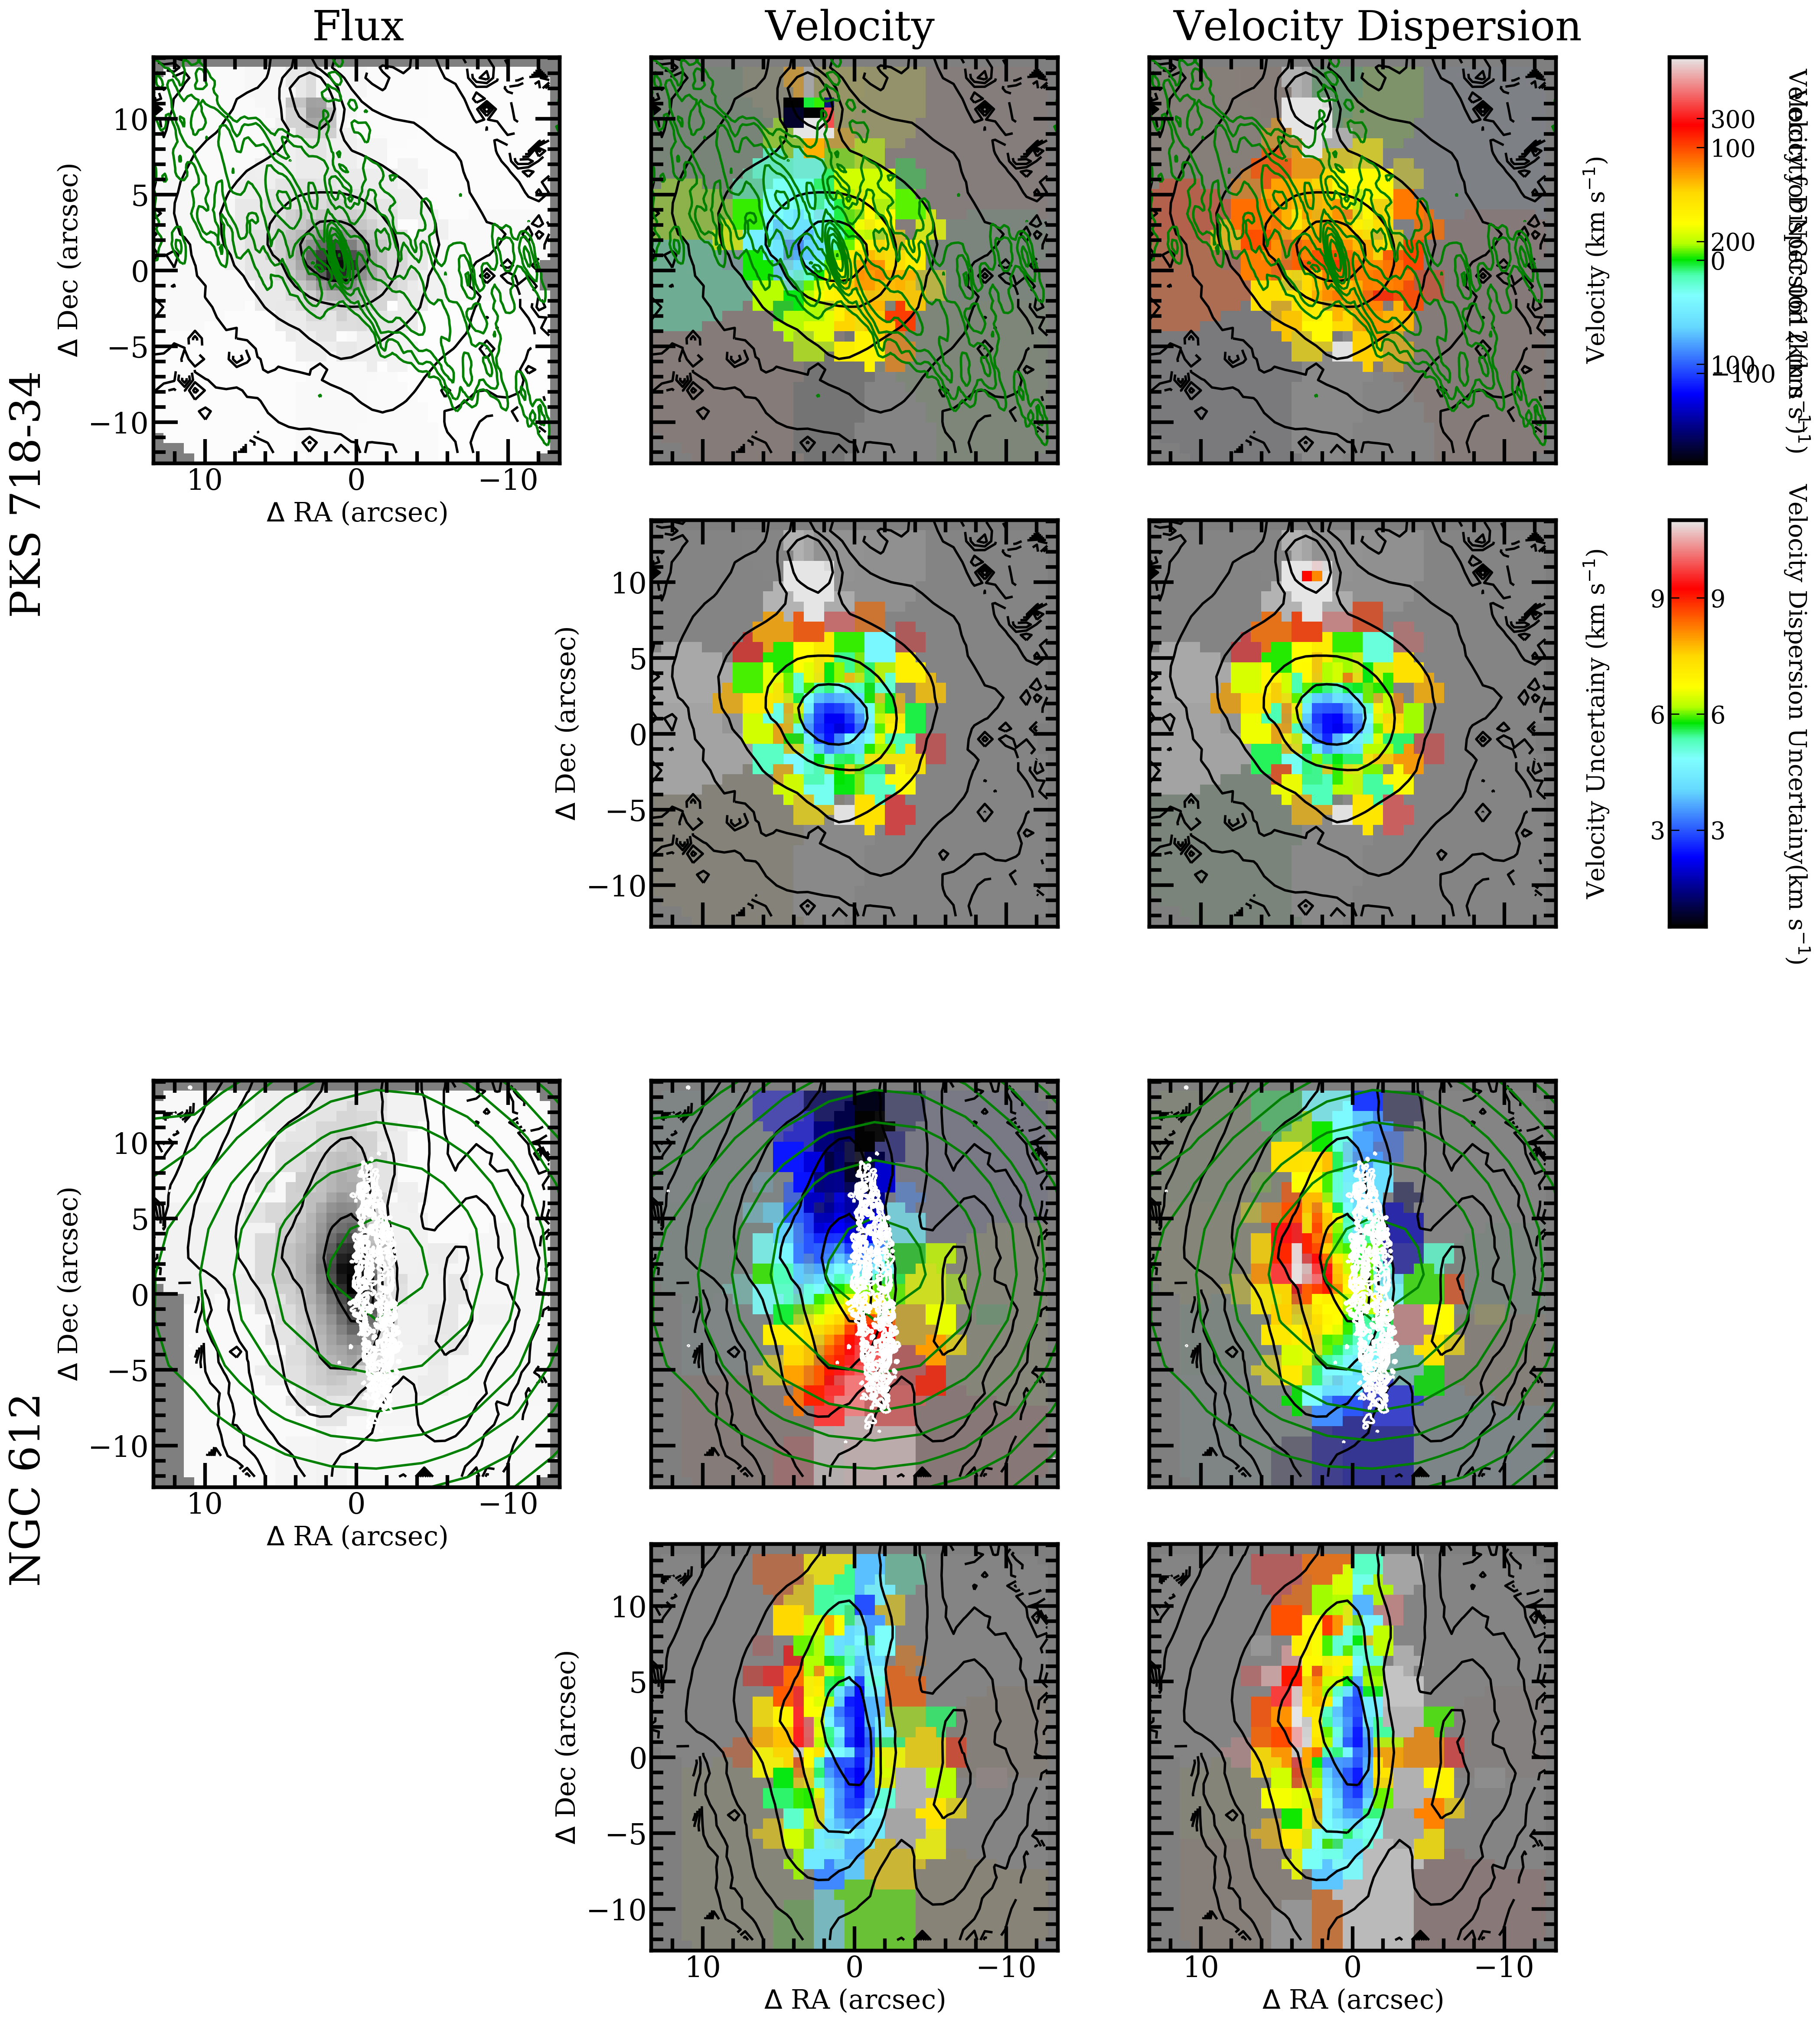
\includegraphics[height=0.62\textheight]{chapter4/vimos/kin4.png}
			\contcaption{\textit{Continued.} The colour scale for the mean velocity map of NGC 612 only is $-322$ to $322 \, \mathrm{km \, s^{-1}}$.}
		\end{figure}

		\begin{figure}
			\centering
			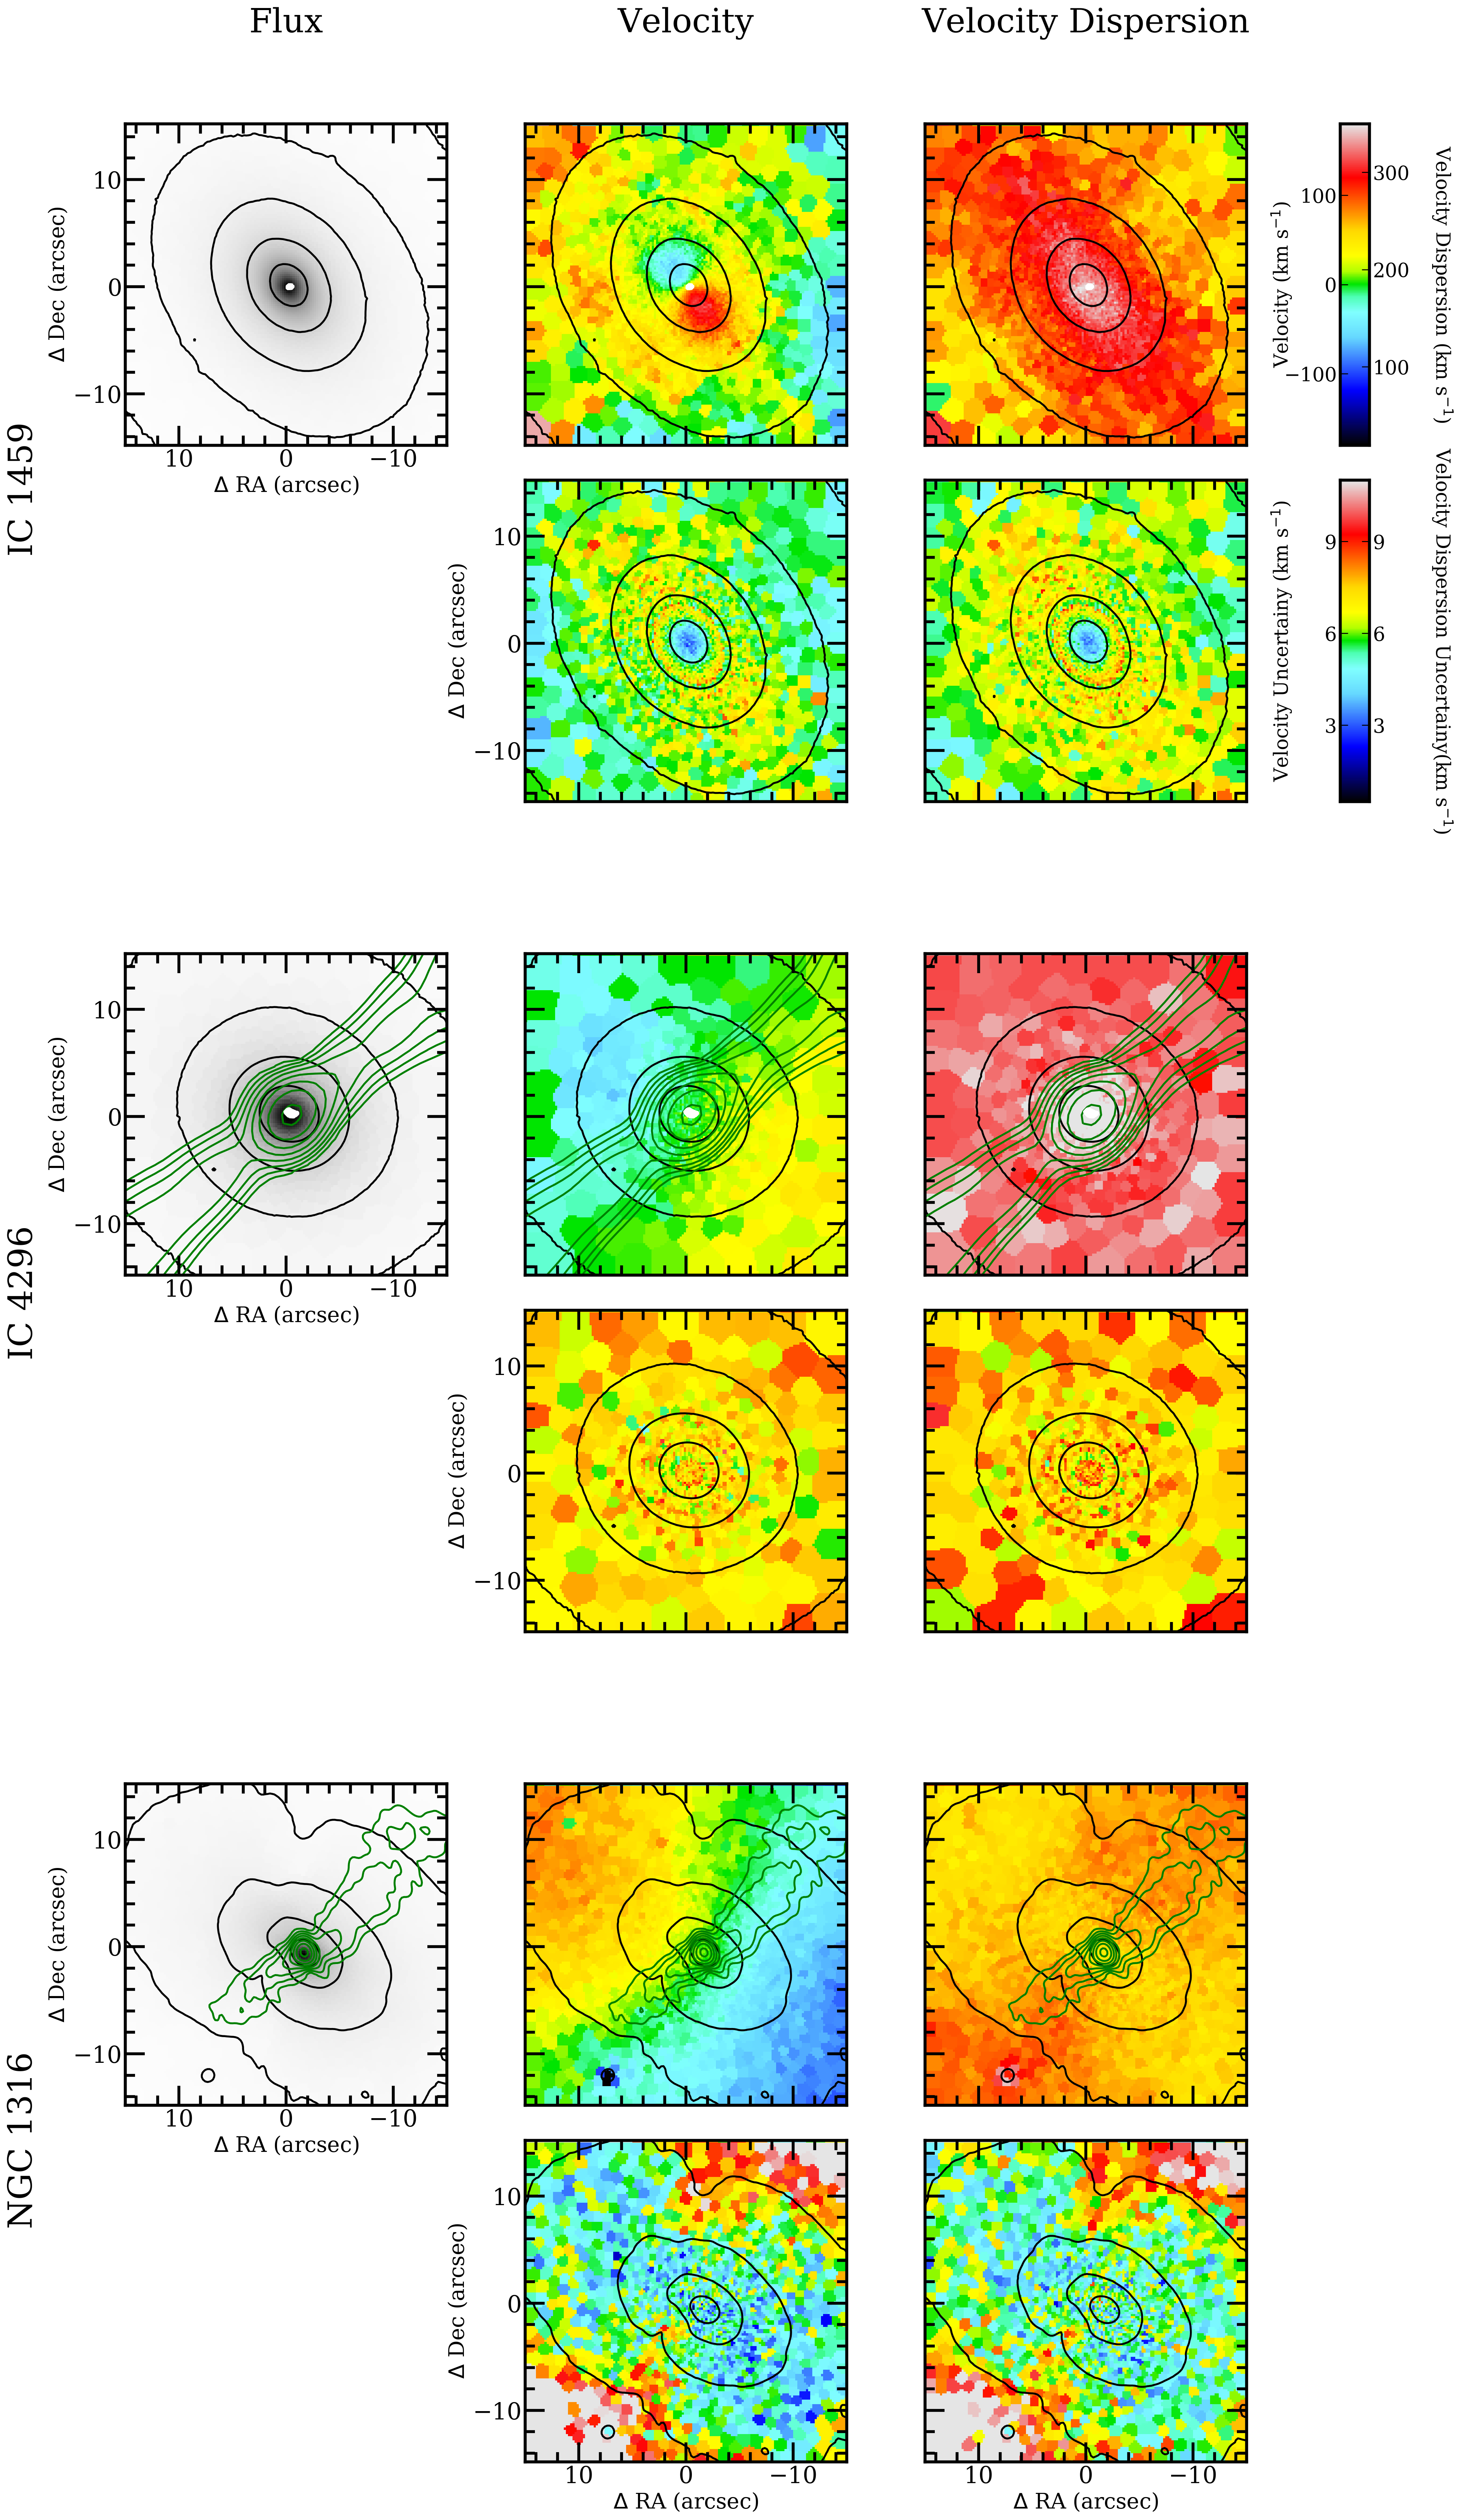
\includegraphics[height=0.94\textheight]{chapter4/muse/kin1.png}
			\caption[MUSE stellar kinematic maps]{As in Figure \ref{fig:VIMOS_stellar} but for the MUSE stellar kinematic maps.}
			\label{fig:MUSE_stellar}
		\end{figure}
		\begin{figure}
			\centering
			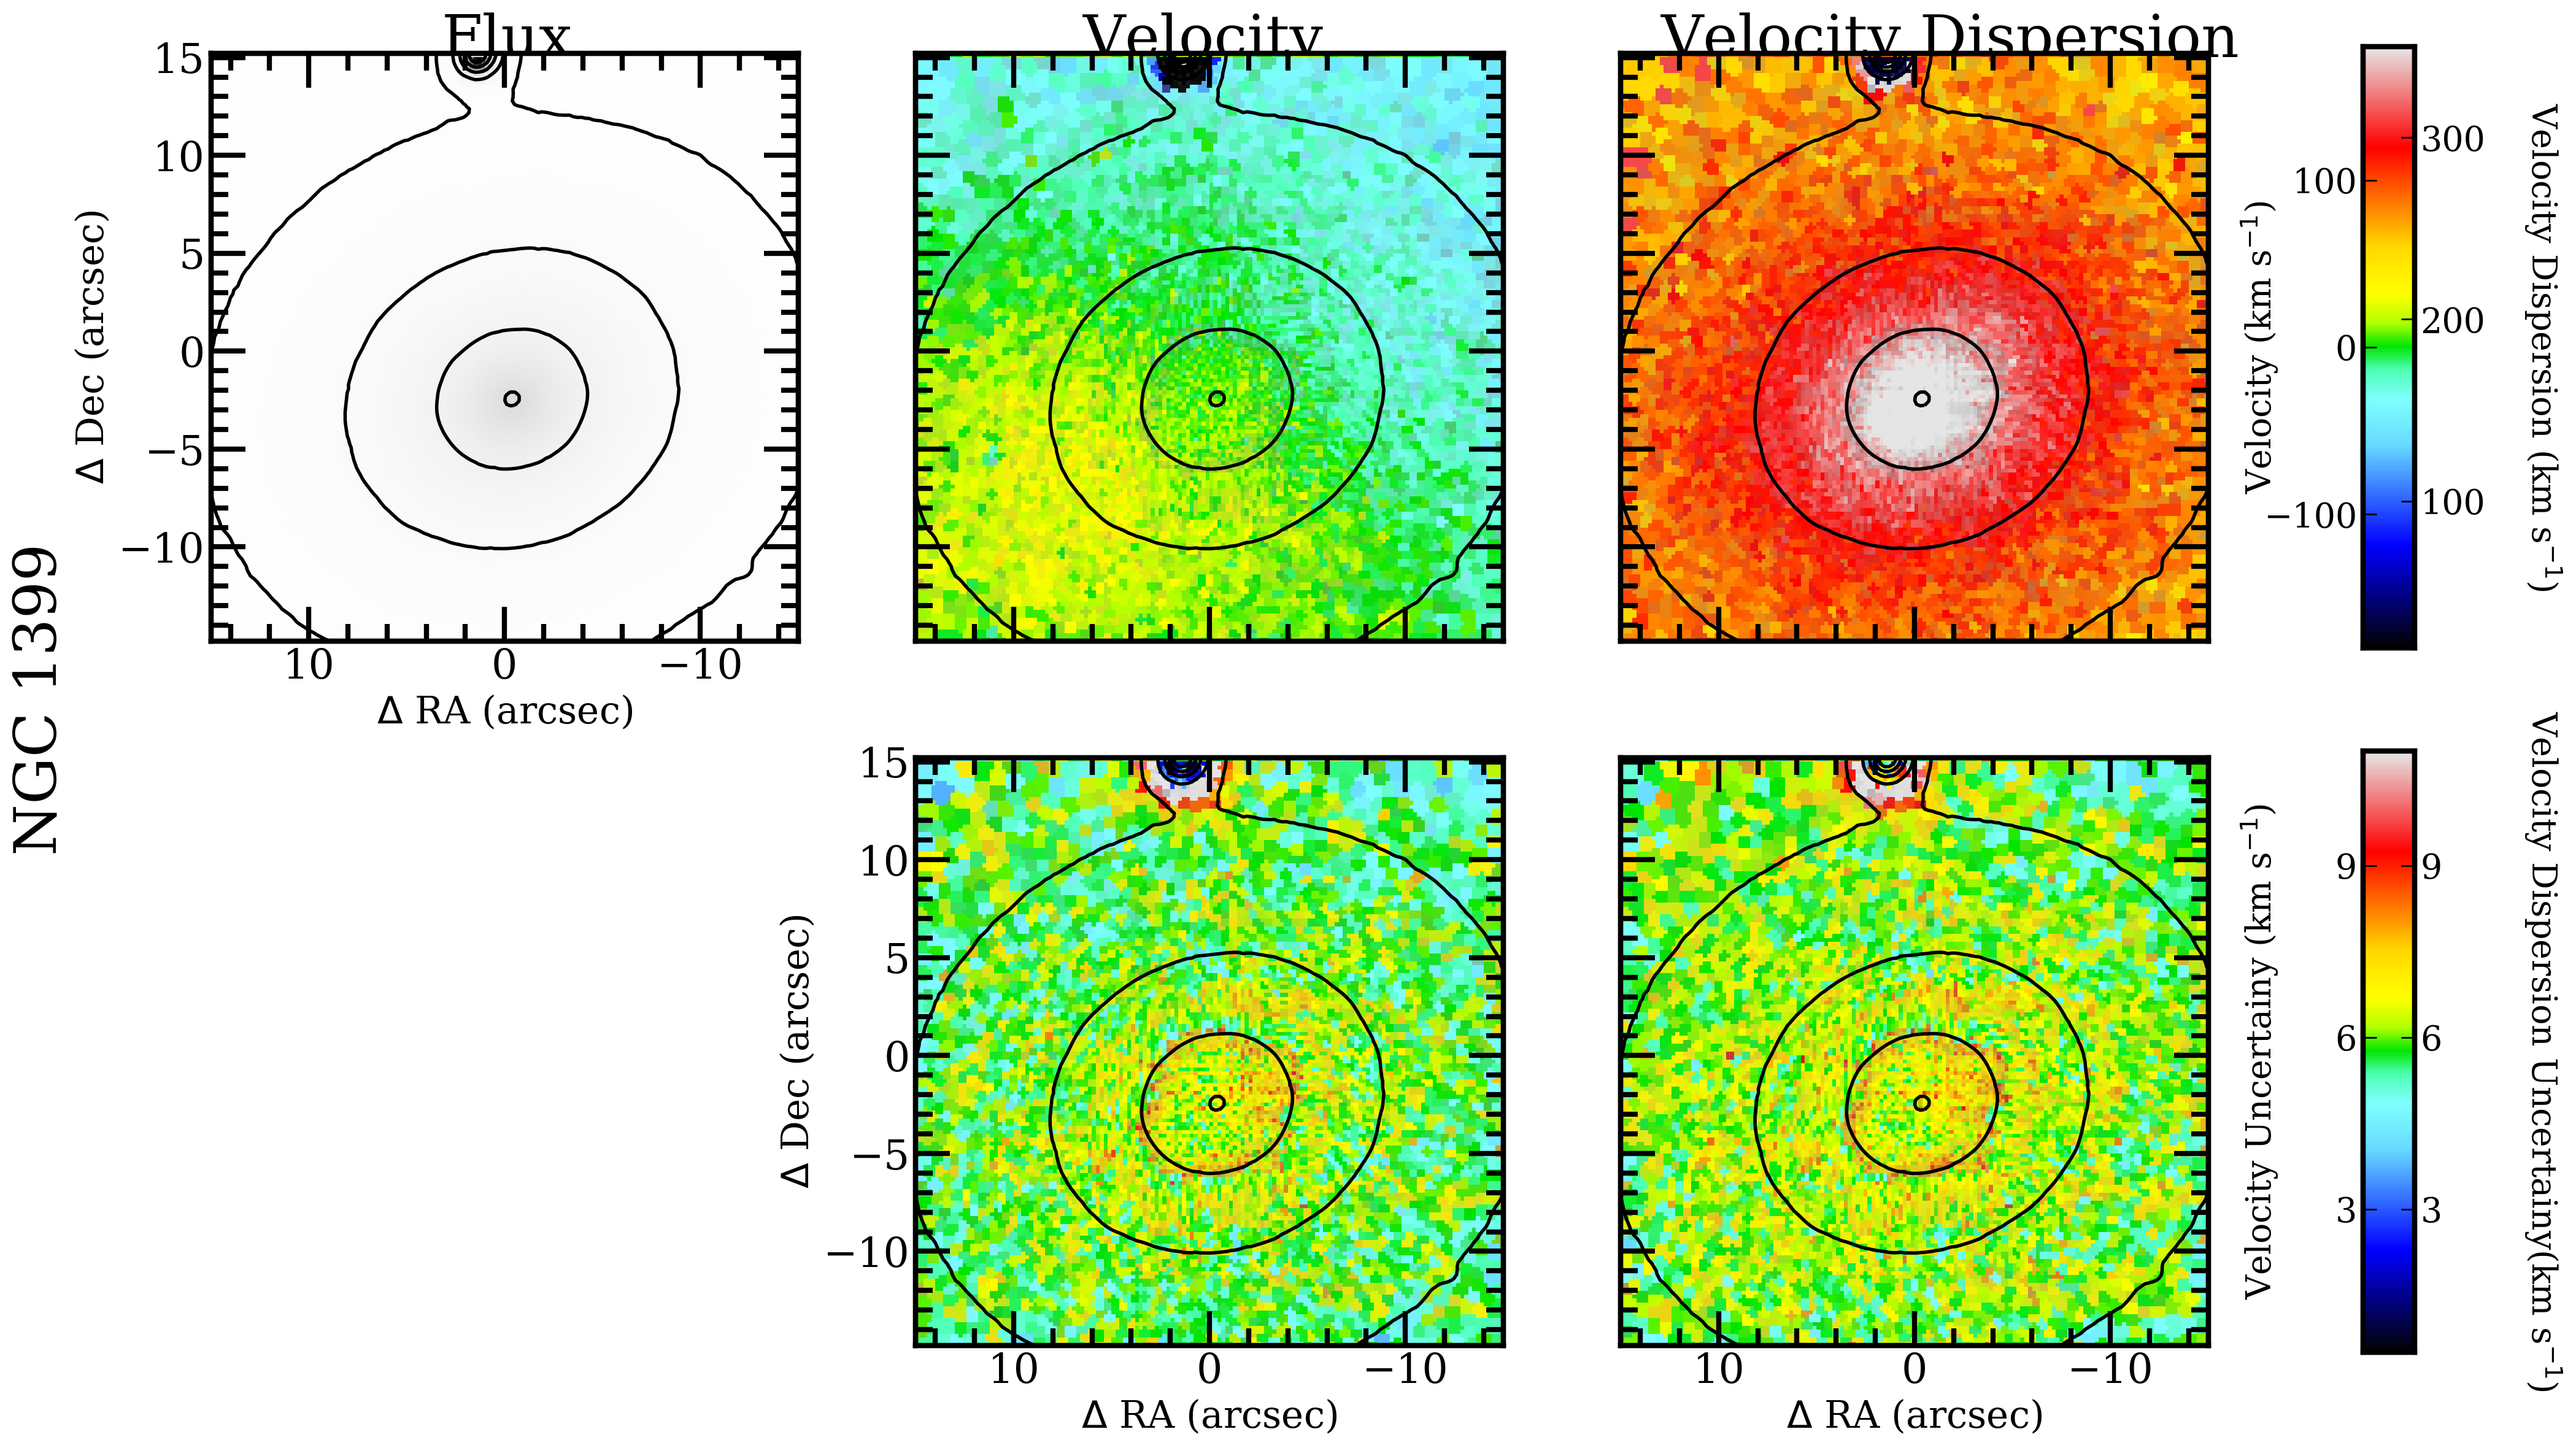
\includegraphics[height=0.31\textheight]{chapter4/muse/kin2.png}
			\contcaption{\textit{Continued.}}
		\end{figure}



		\begin{table}
			\centering
		\begin{threeparttable}
			\caption{Kinematic classifications}
			\label{tab:classify}
			\begin{tabular}{l c c c c c c c}
				\hline
				\hline
				Galaxy		& $\lambda_\mathrm{R_e}$ & $\epsilon_\mathrm{e}$  & $\Gamma_\text{kin}$ (deg) & FR/SR 	& RR/NRR 	& Feature & Group 	\\
				\hline 
				ESO 443-G024 & 0.048 & 0.35 & $-18\pm\leavevmode\phantom{0}2$	& SR & NRR & KDC & c \\
				IC 1459 	& 0.125 & 0.24 & \leavevmode\phantom{0}$-3\pm\leavevmode\phantom{0}1$ & SR & NRR & KDC & c \\
				IC 1531 	& 0.101 & 0.08 & $-54\pm25$	& FR & NRR & LV & a \\
				IC 4296		& 0.034 & 0.03 & \leavevmode\phantom{$-0$}$8\pm12$ & SR &\leavevmode\phantom{N}RR & -- & e \\
				NGC 612 	& 0.655 & 0.36 & \leavevmode\phantom{$-$}$12\pm\leavevmode\phantom{0}6$	& FR &\leavevmode\phantom{N}RR & -- & e \\
				NGC 1316 	& 0.100 & 0.39 & \leavevmode\phantom{$-0$}$6\pm\leavevmode\phantom{0}2$ & FR & NRR & -- & f \\
				NGC 1399 	& 0.090 & 0.12 & $-74\pm\leavevmode\phantom{0}5$ & SR & NRR & LV & a \\
				NGC 3100 	& 0.354 & 0.24 & \leavevmode\phantom{0}$-8\pm\leavevmode\phantom{0}2$ & FR &\leavevmode\phantom{N}RR & -- & e \\
				NGC 3557 	& 0.312 & 0.20 & \leavevmode\phantom{$-$}$16\pm\leavevmode\phantom{0}5$ & FR &\leavevmode\phantom{N}RR & -- & e\\
				NGC 7075 	& 0.068 & 0.04 & \leavevmode\phantom{$-$}$36\pm50$ & SR & NRR & -- & b \\
				PKS 718-34  & 0.159 & 0.17 & \leavevmode\phantom{$-$}$15\pm25$ & FR & NRR & KDC\tnote{a} & b\\
				\hline
				\hline
			\end{tabular}
			\begin{tablenotes}
			\footnotesize
			\note Col.\,1: Galaxy name. Col.\,2: $\lambda_\mathrm{R}$ evaluated at $R_\mathrm{e}$. Col.\,3: Ellipticity at $R_\mathrm{e}$. Col.\,4: Misalignment angle between the kinematic and photometric position angles. Col.\,5: Fast-/slow-rotator (FR/SR) classification. Col.\,6: Regular-rotator (RR) or non-regular-rotator (NRR). Col.\,7: Kinematic features. Col.\,8: Kinematic group.
			\item [a] Tentative classification. A higher signal-to-noise ratio (S/N) in the outer regions of the field of view is required for confirmation.
			\end{tablenotes}
		\end{threeparttable}
		\end{table}

		The stellar kinematics of the sample galaxies are classified according to the regular rotator/non-regular rotator (RR/NRR) categories of \citet{Krajnovic2011}, with the results listed in Col.\,6 of Table \ref{tab:classify}. Here and hereafter, where MUSE datacubes exist their derived properties are quoted. Otherwise the values are derived from the VIMOS datacubes. We find 4/11 of our sample galaxies are regular rotators. This compares to 82\% of the Atlas$^\text{3D}$ sample being classified as regular rotators \citep{Krajnovic2011}. However the likely-hood of a given galaxy being a regular rotator is highly mass dependent with the likely-hood decreasing with increasing mass. Thus since our Southern sample are all extremely massive galaxies, we expect to find a higher fraction of non-regular rotators than the Atlas$^\text{3D}$ survey. 

		In addition to this, we attempt to identify the kinematic features defined by \citet{Krajnovic2011} in an algorithmic way. However, the artefacts from the VIMOS quadrants (see Section \ref{subsec:VIMOSartefacts}) confuse ellipse fitting algorithms so only maps derived from the MUSE data are classified in this way; kinematic features in maps derived from the VIMOS data are identified by eye. These classification are listed in Col.\,7 of Table \ref{tab:classify} and the corresponding kinematic group (see Table \ref{tab:KinGroups} and Fig.\,\ref{fig:EgSubstructure} for group definitions and examples) to which a given galaxy belongs to is given is Col.\,8. We observe 3 KDCs (although PKS 718-34 is only a tentative classification) such that $29\pm19$\% of non-regular rotators in our Southern sample definitely (not including PKS 718-34) contain KDCs (or $43\pm19$\% including PKS 718-34), with the large uncertainty reflecting the low-number statistics. This is consistent with the Atlas$^\text{3D}$ survey who found find $25\pm7$\% of non-regular rotators host KDCs \citep{Krajnovic2011}.


		\subsection{Ellipticity}
			\label{subsec:Ellipticity}

			\begin{figure}
				\centering
				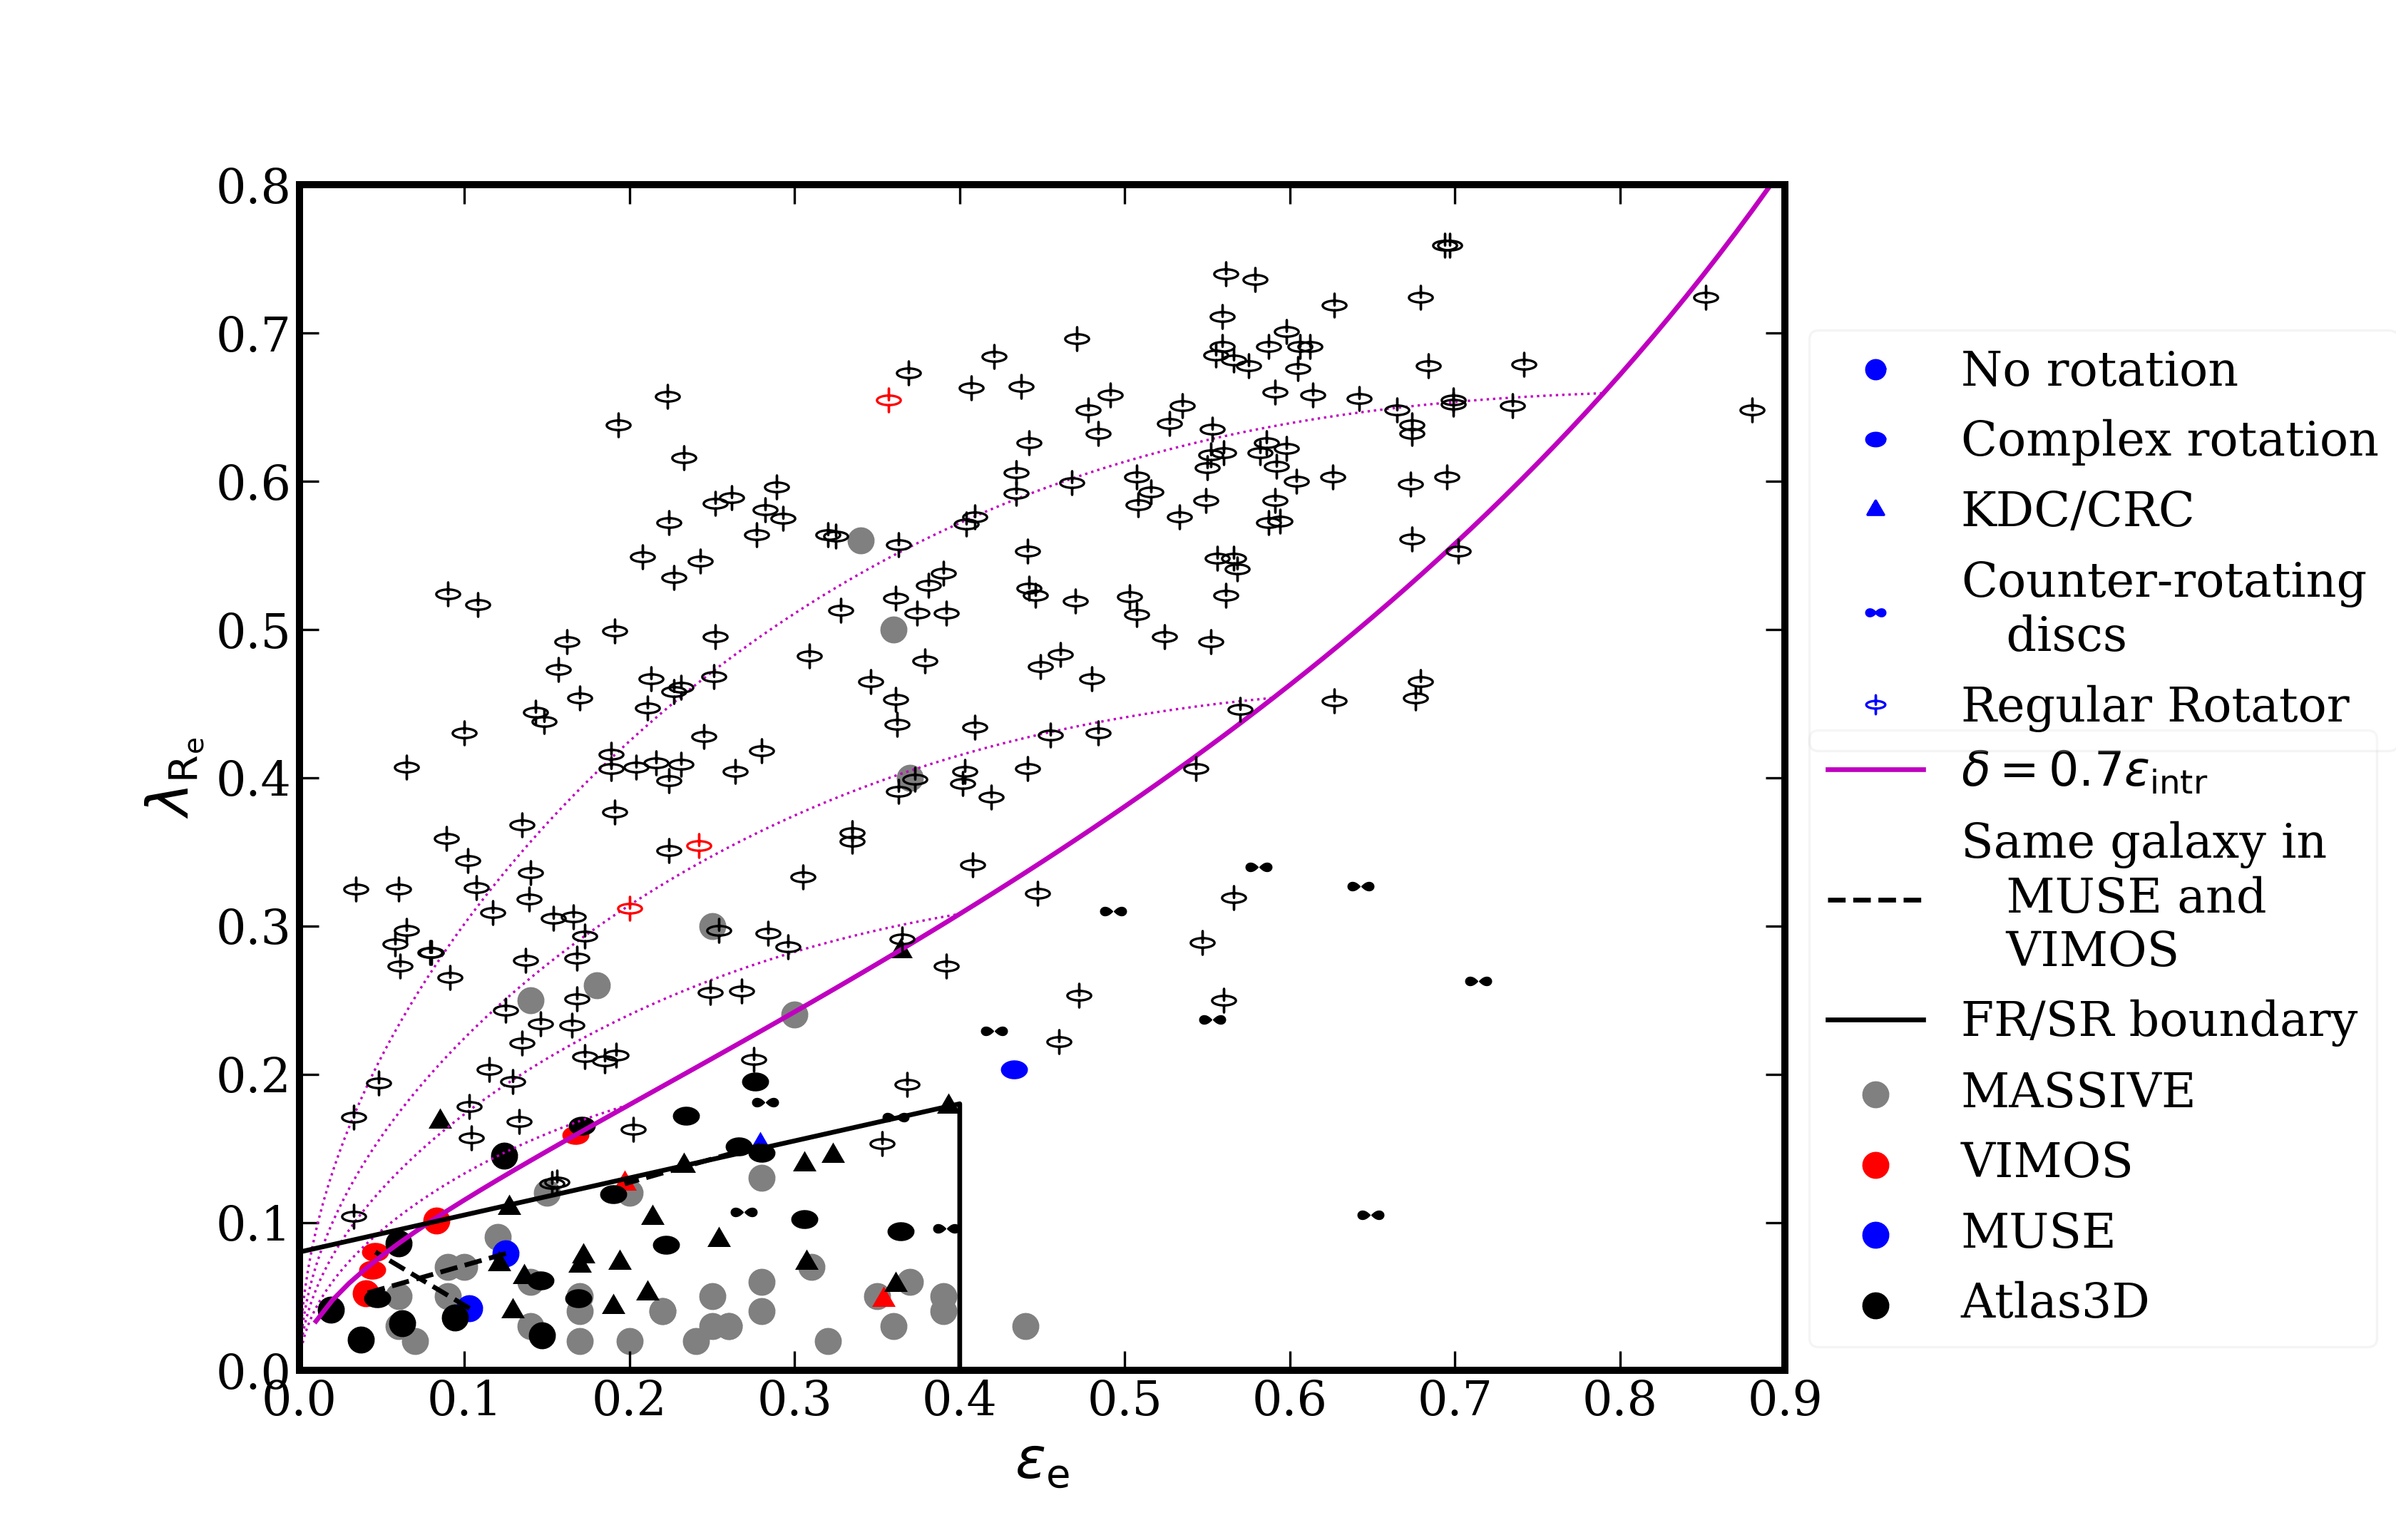
\includegraphics[width=.9\textwidth]{chapter4/lambda_R_ellipticity.png}
				\caption[$\lambda_\mathrm{R_e}$ -- ellipticity diagram]{$\lambda_\mathrm{R_e}$ -- ellipticity diagram. VIMOS and MUSE measurements are shown in red and blue, respectively. For comparison, Atlas$^\text{3D}$ galaxies \citep{Emsellem2011} are shown in black and MASSIVE galaxies \citep{Veale2017} in grey. The theoretical limit (edge-on systems) of disc-dominated galaxies is shown in solid magenta, with lines of constant intrinsic angular momentum but varying inclination in dotted magenta. The black solid lines show the limits of the fast-/slow-rotator classes. The MASSIVE survey does not report substructure, so the MASSIVE sample galaxies are shown with filled circles.}
				\label{fig:lambdaR_ellip}
			\end{figure}

			Ellipticity is measured as the ellipticity of the best-fitting ellipse to the surface-brightness map with an mean radius $R_\mathrm{m}$, of 1 effective radius $R_\mathrm{e}$. Firstly the centre of the galaxy is found as the luminosity weighted centre using the \textsc{python} routine \textsc{find\_galaxy}, which is part of the \textsc{mge} package\footnote{\url{http://www-astro.physics.ox.ac.uk/\~mxc/software/}} by \citet{Cappellari2002}. This is then used as an input for the \textsc{idl} routine \textsc{kinemetry}\footnote{\url{http://davor.krajnovic.org/idl/}} by \citet{Krajnovic2006} which finds the best-fitting ellipses at a range of evenly spaced semi-major axes. This is achieved by performing harmonic expansion of maps along ellipses with a given semi-major axis and, when used for even moments (e.g.\ surface brightness, velocity dispersion, h$_4$ etc.), minimising the amplitude of the first and second harmonics. The results include the ellipticity, $\epsilon$ and position angle $PA_\text{phot}$ of the best-fitting ellipse for each semi-major axis. The fit is repeated for increasing semi-major axis until $<$75\% of the ellipse is not contained within the field of view.

			In reality, the field of view does not always contain 1 $R_\mathrm{e}$. Where this is the case, we follow the method by \citet{Emsellem2007}, were $R_\mathrm{m}$ is redefined as $R_\mathrm{m} \equiv \sqrt{A_\mathrm{s}/\pi}$, where $A_\mathrm{s}$ is the area of the ellipse contained within the field of view. For a given galaxy, we fit ellipses as described above, up to $R_\mathrm{m} = R_\mathrm{max}$, where $A_\mathrm{s}$ reaches a maximum difference if 15\% to the area of the fitted ellipse, $A_\text{ellipse}$. The value $\epsilon_\mathrm{e}$, the ellipticity at 1 $R_\mathrm{e}$ or $R_\text{max}$, whichever is smallest, is given in Table \ref{tab:classify}. 

		\subsection{Fast-/Slow-Rotator Classification}
			\label{subsec:FSRot}

			The specific angular momentum parameter $\lambda_R$ (see Section \ref{sec:ETG} for for definitions of $\lambda_R$) is evaluated at 1 $R_\mathrm{e}$ or $R_\text{max}$, whichever is smaller (as described for ellipticity in Section \ref{subsec:Ellipticity}), and is given in Table \ref{tab:classify}. This is plotted against the ellipticity, $\epsilon_\mathrm{e}$ (see Section \ref{subsec:Ellipticity}) in Fig.\,\ref{fig:lambdaR_ellip}. This plot shows the classification scheme of \citet{Cappellari2016} for the fast-/slow-rotator (FR/SR) categories (originally defined by \citealt{Emsellem2011}, but later refined by \citealt{Cappellari2016}; see Section \ref{sec:ETG}). This classification is given in Col.\,5 of Table \ref{tab:classify}.

			We find that 5 out of 11 galaxies, or $(45\pm13)$\%, are slow rotators. This is between that of the Atlas$^\text{3D}$ and MASSIVE projects, who find 13.1\% and 77.5\% of their sample galaxies to be slow rotators, respectively. However, slow rotators are more likely to be found in higher mass galaxies and the three samples (Atlas$^\text{3D}$, MASSIVE and our Southern sample) have very different mass distributions (see upper panel of Fig.\,\ref{fig:SRmassFraction}).

			In order to account for the difference in mass distribution, we find the expected fraction of slow rotators in the Southern sample, $f'$, corrected to the mass distribution of the combined Atlas$^\text{3D}$ and MASSIVE samples (hereafter the A+M sample), as
			\begin{equation}
				f' = \sum_{i=0}^N N^\mathrm{SS}_i f^\mathrm{AM}_i \, , 
			\end{equation}
			where $N^\mathrm{SS}_i$ is the number of Southern sample galaxies in the $i^\mathrm{th}$ mass bin, $N^\mathrm{AM}_i$ is the fraction of slow rotators in the $i^\mathrm{th}$ mass bin in the A+M combined sample and $N$ is the total number of mass bins. In our case we use the $K$-band absolute magnitude ($M_K$) as a proxy for stellar mass, with bins of 0.5 mag. This gives an expected fraction of $f' = 0.64 \pm 0.06$, just consistent with our finding of $(45\pm13)$\% of the Southern sample galaxies being slow rotators. Again the large uncertainty reflects the low number statistics of the Southern sample. There is, therefore, no discernible difference in the fraction of galaxies that are slow-rotators between our radio-selected Southern sample and the optically-selected A+M sample, once differences in the mass distributions are taken into account. 

			\begin{figure}
				\centering
				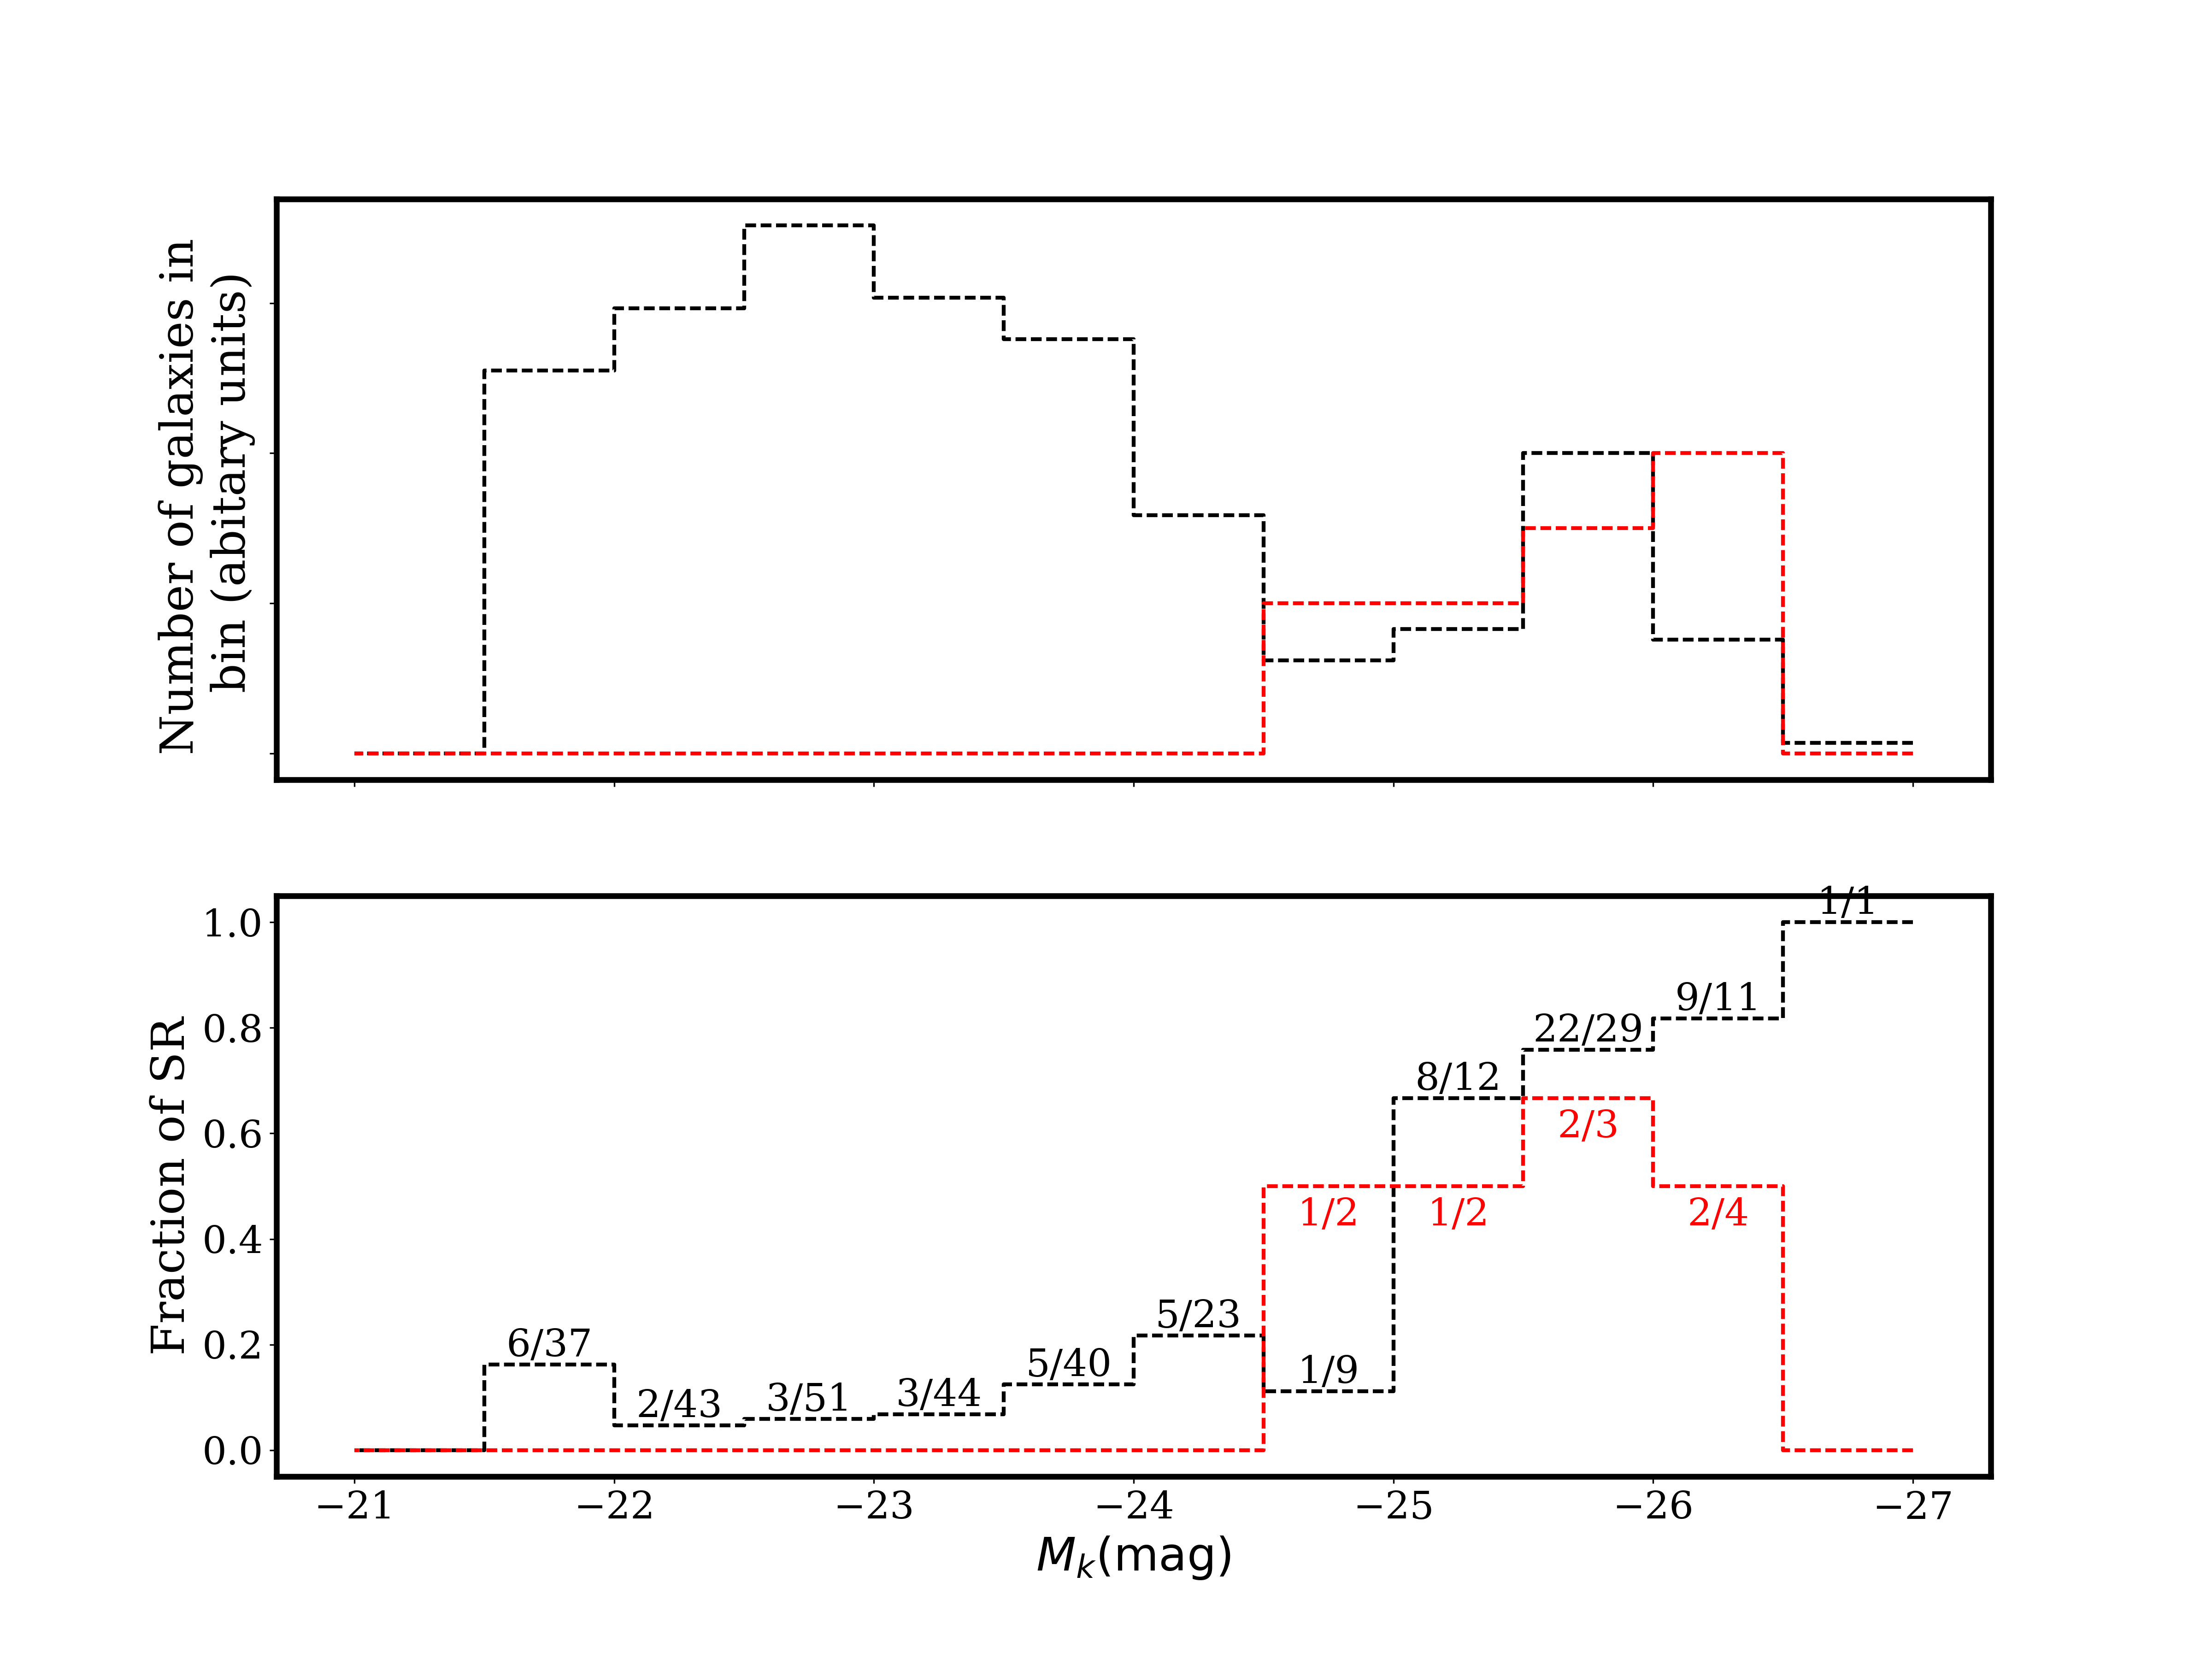
\includegraphics[width=0.8\textwidth]{chapter4/M_k_binned.png}
				\caption[Mass matching global kinematics]{Upper panel: mass distribution of the A+M sample (black) and of our Southern sample (red). Lower panel: fraction of slow rotators within each mass bin. The labels list the number of slow rotators and total number of galaxies in each bin.}
				\label{fig:SRmassFraction}
			\end{figure}

		\subsection{Radial Angular Momentum Profile}
			\label{subsec:ResolvedLambda_R}
			The radial $\lambda_R$ profiles (i.e.\ $\lambda_R$ as a function of aperture radius) are shown in Fig.\,\ref{fig:lambdaR_profile}. We see, with the exception of IC 1531, a disc with very low inclination, fast and slow rotators are separated by $\approx 0.3\,\mathrm{R_\odot}$. We also see that most of the fast rotators of our Southern sample have a rapidly rising $\lambda_R$ profile, which flatten out by $\approx 0.5\,\mathrm{R_\odot}$. This is consistent with the SAURON surveys findings \citep[e.g.][Fig.\,2]{Emsellem2007}. 

			\begin{figure}
				\centering
				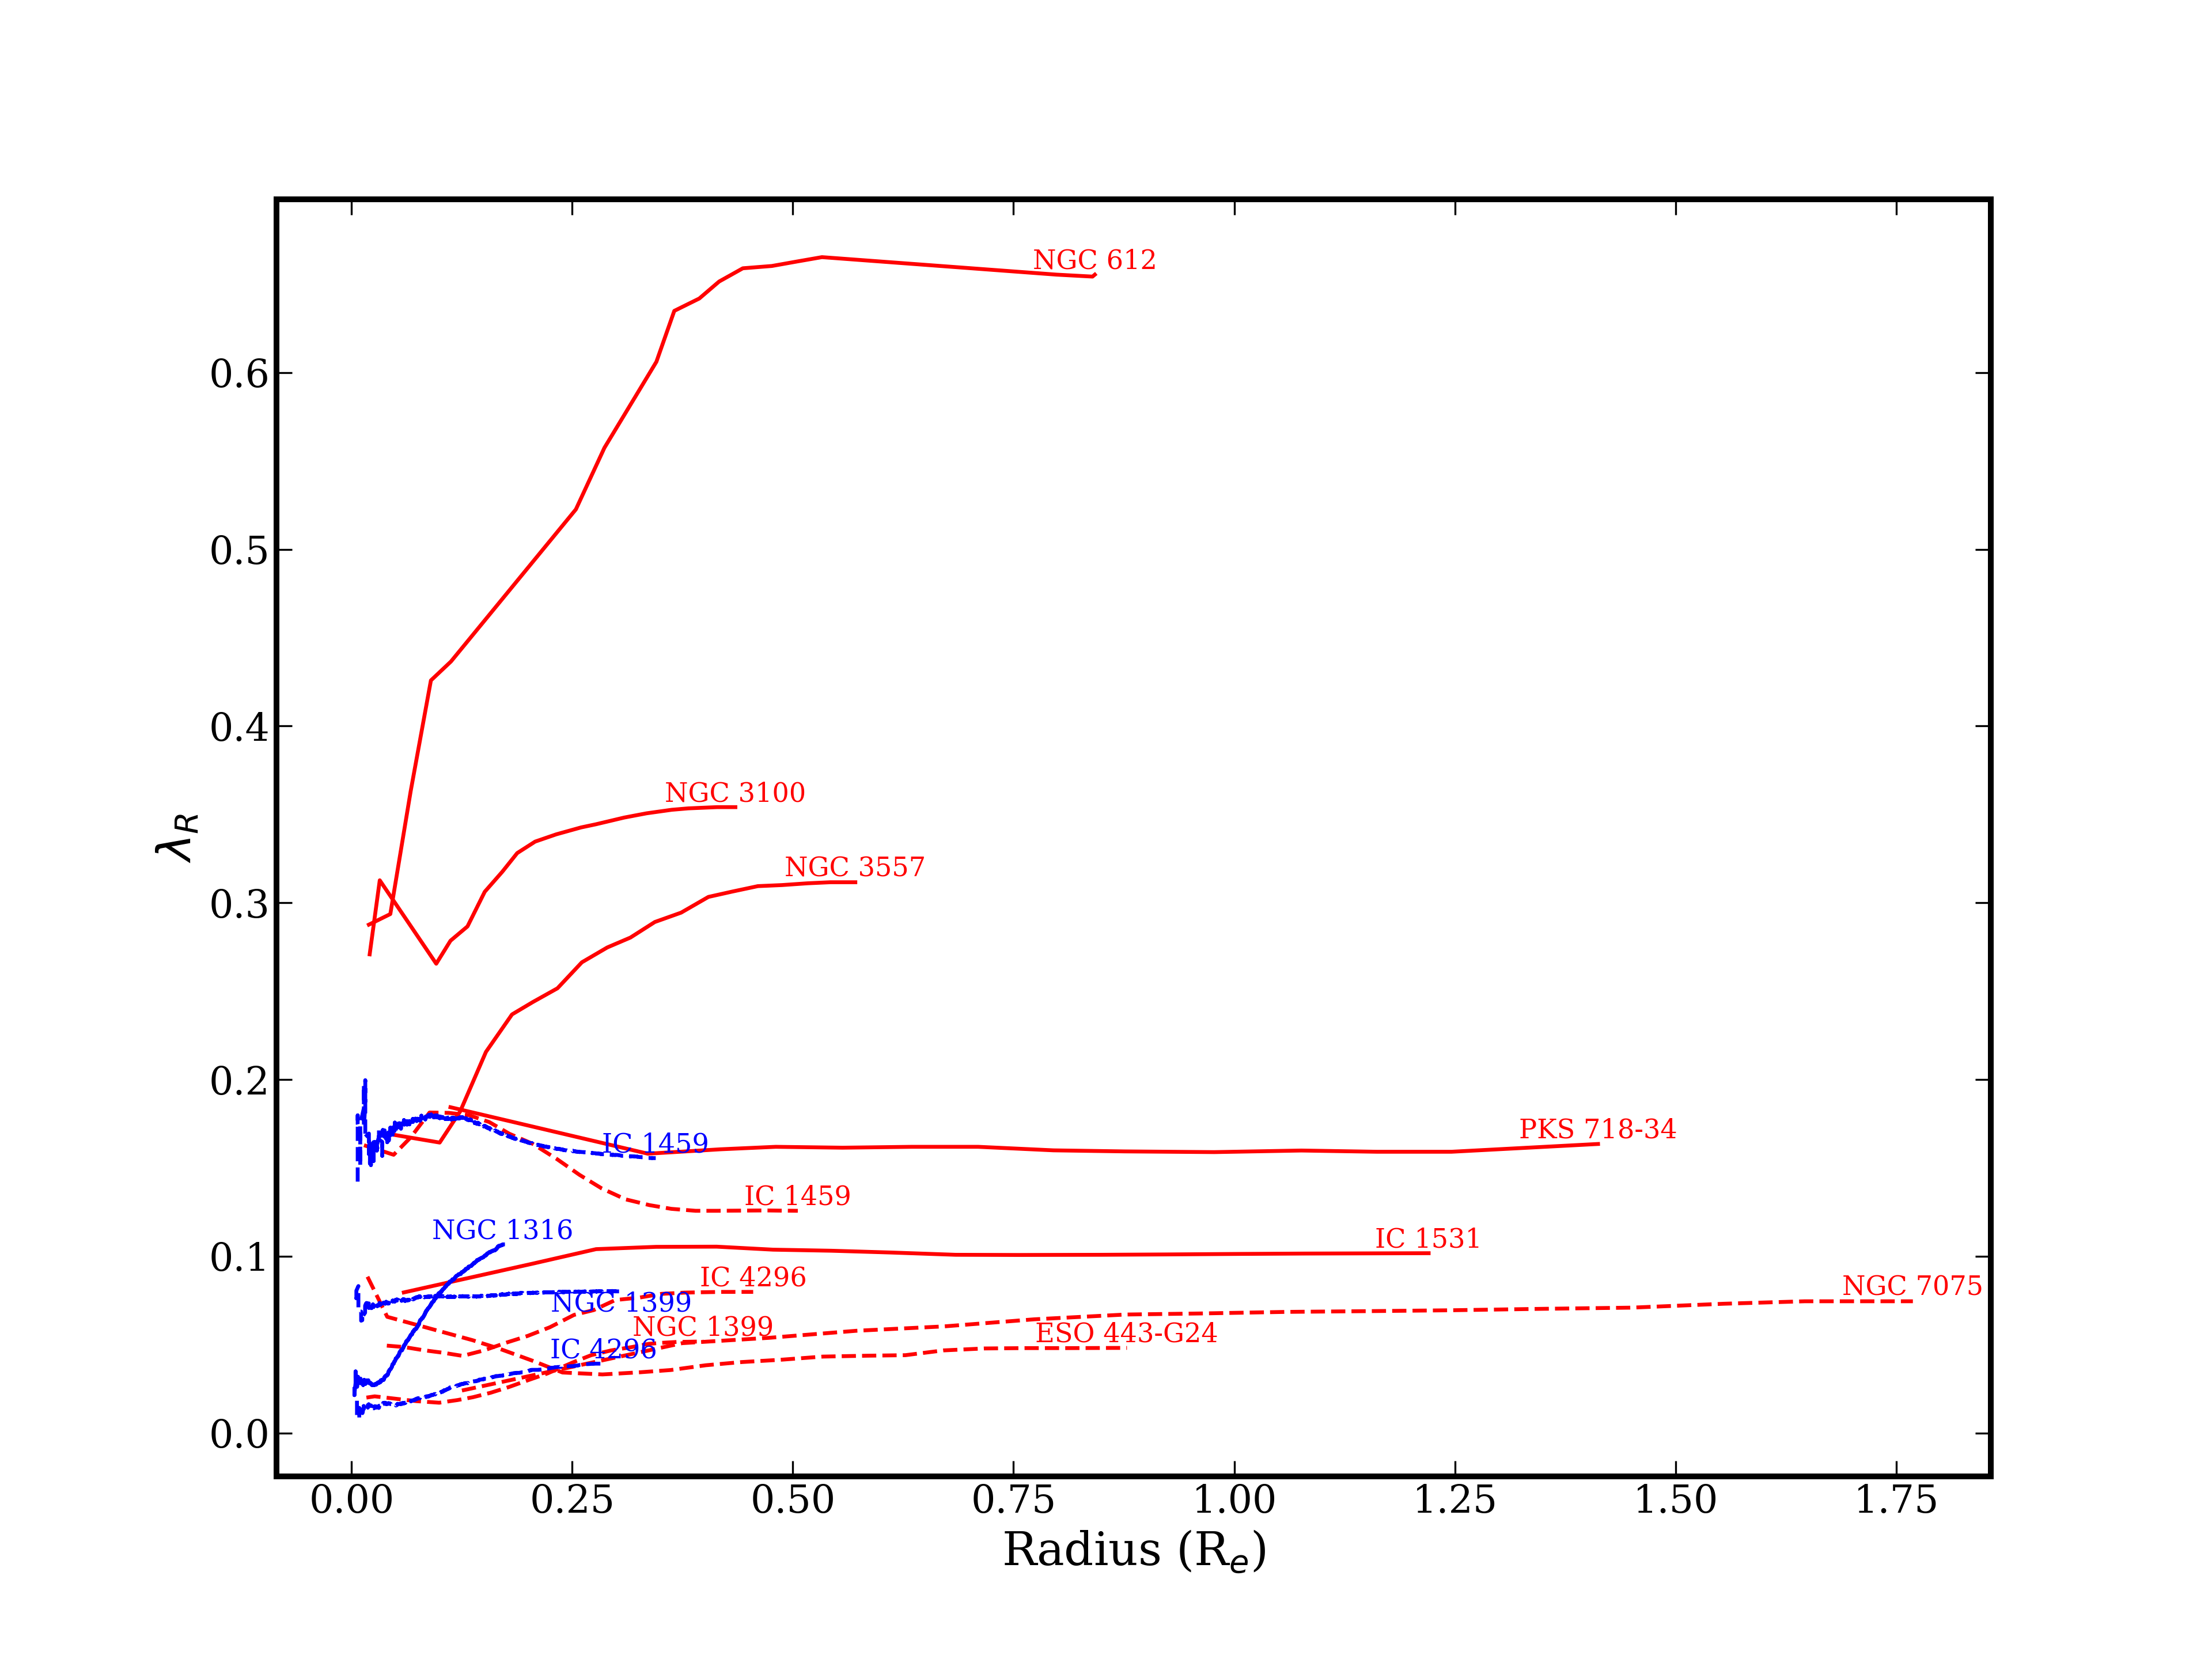
\includegraphics[width=.7\textwidth]{chapter4/lambda_R.png}
				\caption[$\lambda_{R}$ radial profiles]{Radial $\lambda_{R}$ profiles. Profiles derived from VIMOS data are in blue, while those derived from MUSE data are in red. Solid lines represent fast rotators; dashed lines, slow rotators.}
				\label{fig:lambdaR_profile}
			\end{figure}

		
		\subsection{Intrinsic Shape}
			\label{subsec:Misalignment}

			The photometric position angle, $PA_\text{phot}$, is defined as the angle westwards from North of semi-major axis of the largest best-fitting ellipse as found in Section \ref{subsec:Ellipticity}. The kinematic position angle, $PA_\text{kin}$, is defined as the angle of the axis perpendicular to the apparent angular momentum vector westwards from North. A global value of $PA_\text{kin}$ is found using the \textsc{python} routine \textsc{fit\_kinematic\_pa}\footnote{\url{http://www-astro.physics.ox.ac.uk/\~mxc/software/\#pa\_kin}} as described in appendix C of \citet{Krajnovic2006}. This routine finds a symmetric (about $PA_\text{kin}$) velocity field, by replacing the mean velocity, $V$, in each bin with
			\begin{equation}
				V'(x, y) = \frac{V(x,y) + V(x, -y) - V(-x,y) - V(-x,-y))}{4} \,,
			\end{equation}
			where $x$ and $y$ are the centroid coordinates of a given bin, with the origin at the centre of the galaxy and the x axis aligned along $PA_\text{kin}$. Linear interpolation is used where necessary.

			Column 4 in Table \ref{tab:classify} lists the misalignments between the photometric and kinematic position angles, $\Gamma_\text{kin} \equiv \arcsin(\sin[PA_\text{phot} - PA_\text{kin}])$. Misaligned systems may appear aligned in certain projections (though aligned systems will be aligned in all projections) and as such $\Gamma_\text{kin}$ cannot be used to describe the intrinsic shape of an individual galaxy, but, as described in Section \ref{sec:ETG}, it can be used in a statistical manner. We find all the regular rotators in our Southern sample, are consistent with having aligned photometry and kinematic position angles to within 11\degree, while non-regular rotators have a large range of values of $\Gamma_\text{kin}$. IC 1531, NGC7075 and PKS 718-34 all have very large uncertainties in the value of $PA_\text{phot}$ due to the VIMOS quadrant artefacts causing the fitting routine of \textsc{kinemetry} to become unreliable. 

			The lack of misalignments in regular rotators is consistent with \citet{Cappellari2007}, \citet{Krajnovic2011} and \citet{Fogarty2015}, who all showed that regular rotators almost always have aligned photometric and kinematic axes with very little scatter and that regular rotators with a significant misalignment are either interacting or strongly barred. The lack of misalignments suggests that the regular rotators (including those within our Southern sample) are consistent with being axisymmetric \citep{Cappellari2016}.

			Misalignments between the photometric and kinematic position angles are routinely observed for non-regular rotators. This generally implies a more triaxial intrinsic shape, although large misalignments are extremely rarely observed in galaxies with $\epsilon > 0.4$, suggesting that non-regular rotators are more spherical in shape \citep{Cappellari2016}. The non-regular rotators in our Southern sample indeed all have $\epsilon < 0.4$ showing that they are consistent with a fairly spherical, triaxial intrinsic shape.


\section{Stellar Population}
	\label{sec:pop}
	As described in Section \ref{subsec:PopFit}, in order to find the best-fitting stellar populations for our Southern sample, we must first measure the absorption line strengths of the indices in Table \ref{tab:abIndex}. We first present maps of the strength of each index (Section \ref{subsec:absorption}), before examining the Mg -- $\sigma$ relation (Section \ref{subsubssec:Mgsigma}), comparing the measured line strengths to the literature (Section \ref{subsubsec:Lit}) and finally presenting maps of the stellar populations (Section \ref{subsec:ssp}).

	\subsection{Absorption Line Strengths}
		\label{subsec:absorption}

		Figs.\,\ref{fig:VIMOS_absorption} and \ref{fig:MUSE_absorption} show the spatially-resolved absorption line strengths of our Southern sample galaxies. For the VIMOS datacubes, we measure the G4300, Fe4383, Ca4455, Fe4531, H\,$\beta$, Fe5015 and Mg\,b indices, as defined in Table \ref{tab:abIndex}. For the most distant galaxies (NGC 612 and PKS 718-34), the red continuum band of the Mg\,b is redshifted beyond the spectral range of the VIMOS spectrograph. In these cases we have not attempted to adjust the definition of the Mg\,b index bandpass (as \citealt{Kuntschner2006} did with defining Fe5270s to use instead of Fe5270), but have simply not included Mg\,b in any future analysis of these galaxies. For the MUSE datacubes, we measure the H\,$\beta$, Fe5015, Mg\,b, Fe5270, Fe5335, Fe5406, Fe5709, Fe5782, NaD, TiO1 and TiO2 indices, also defined in Table \ref{tab:abIndex}.

		\begin{figure}
			\centering
			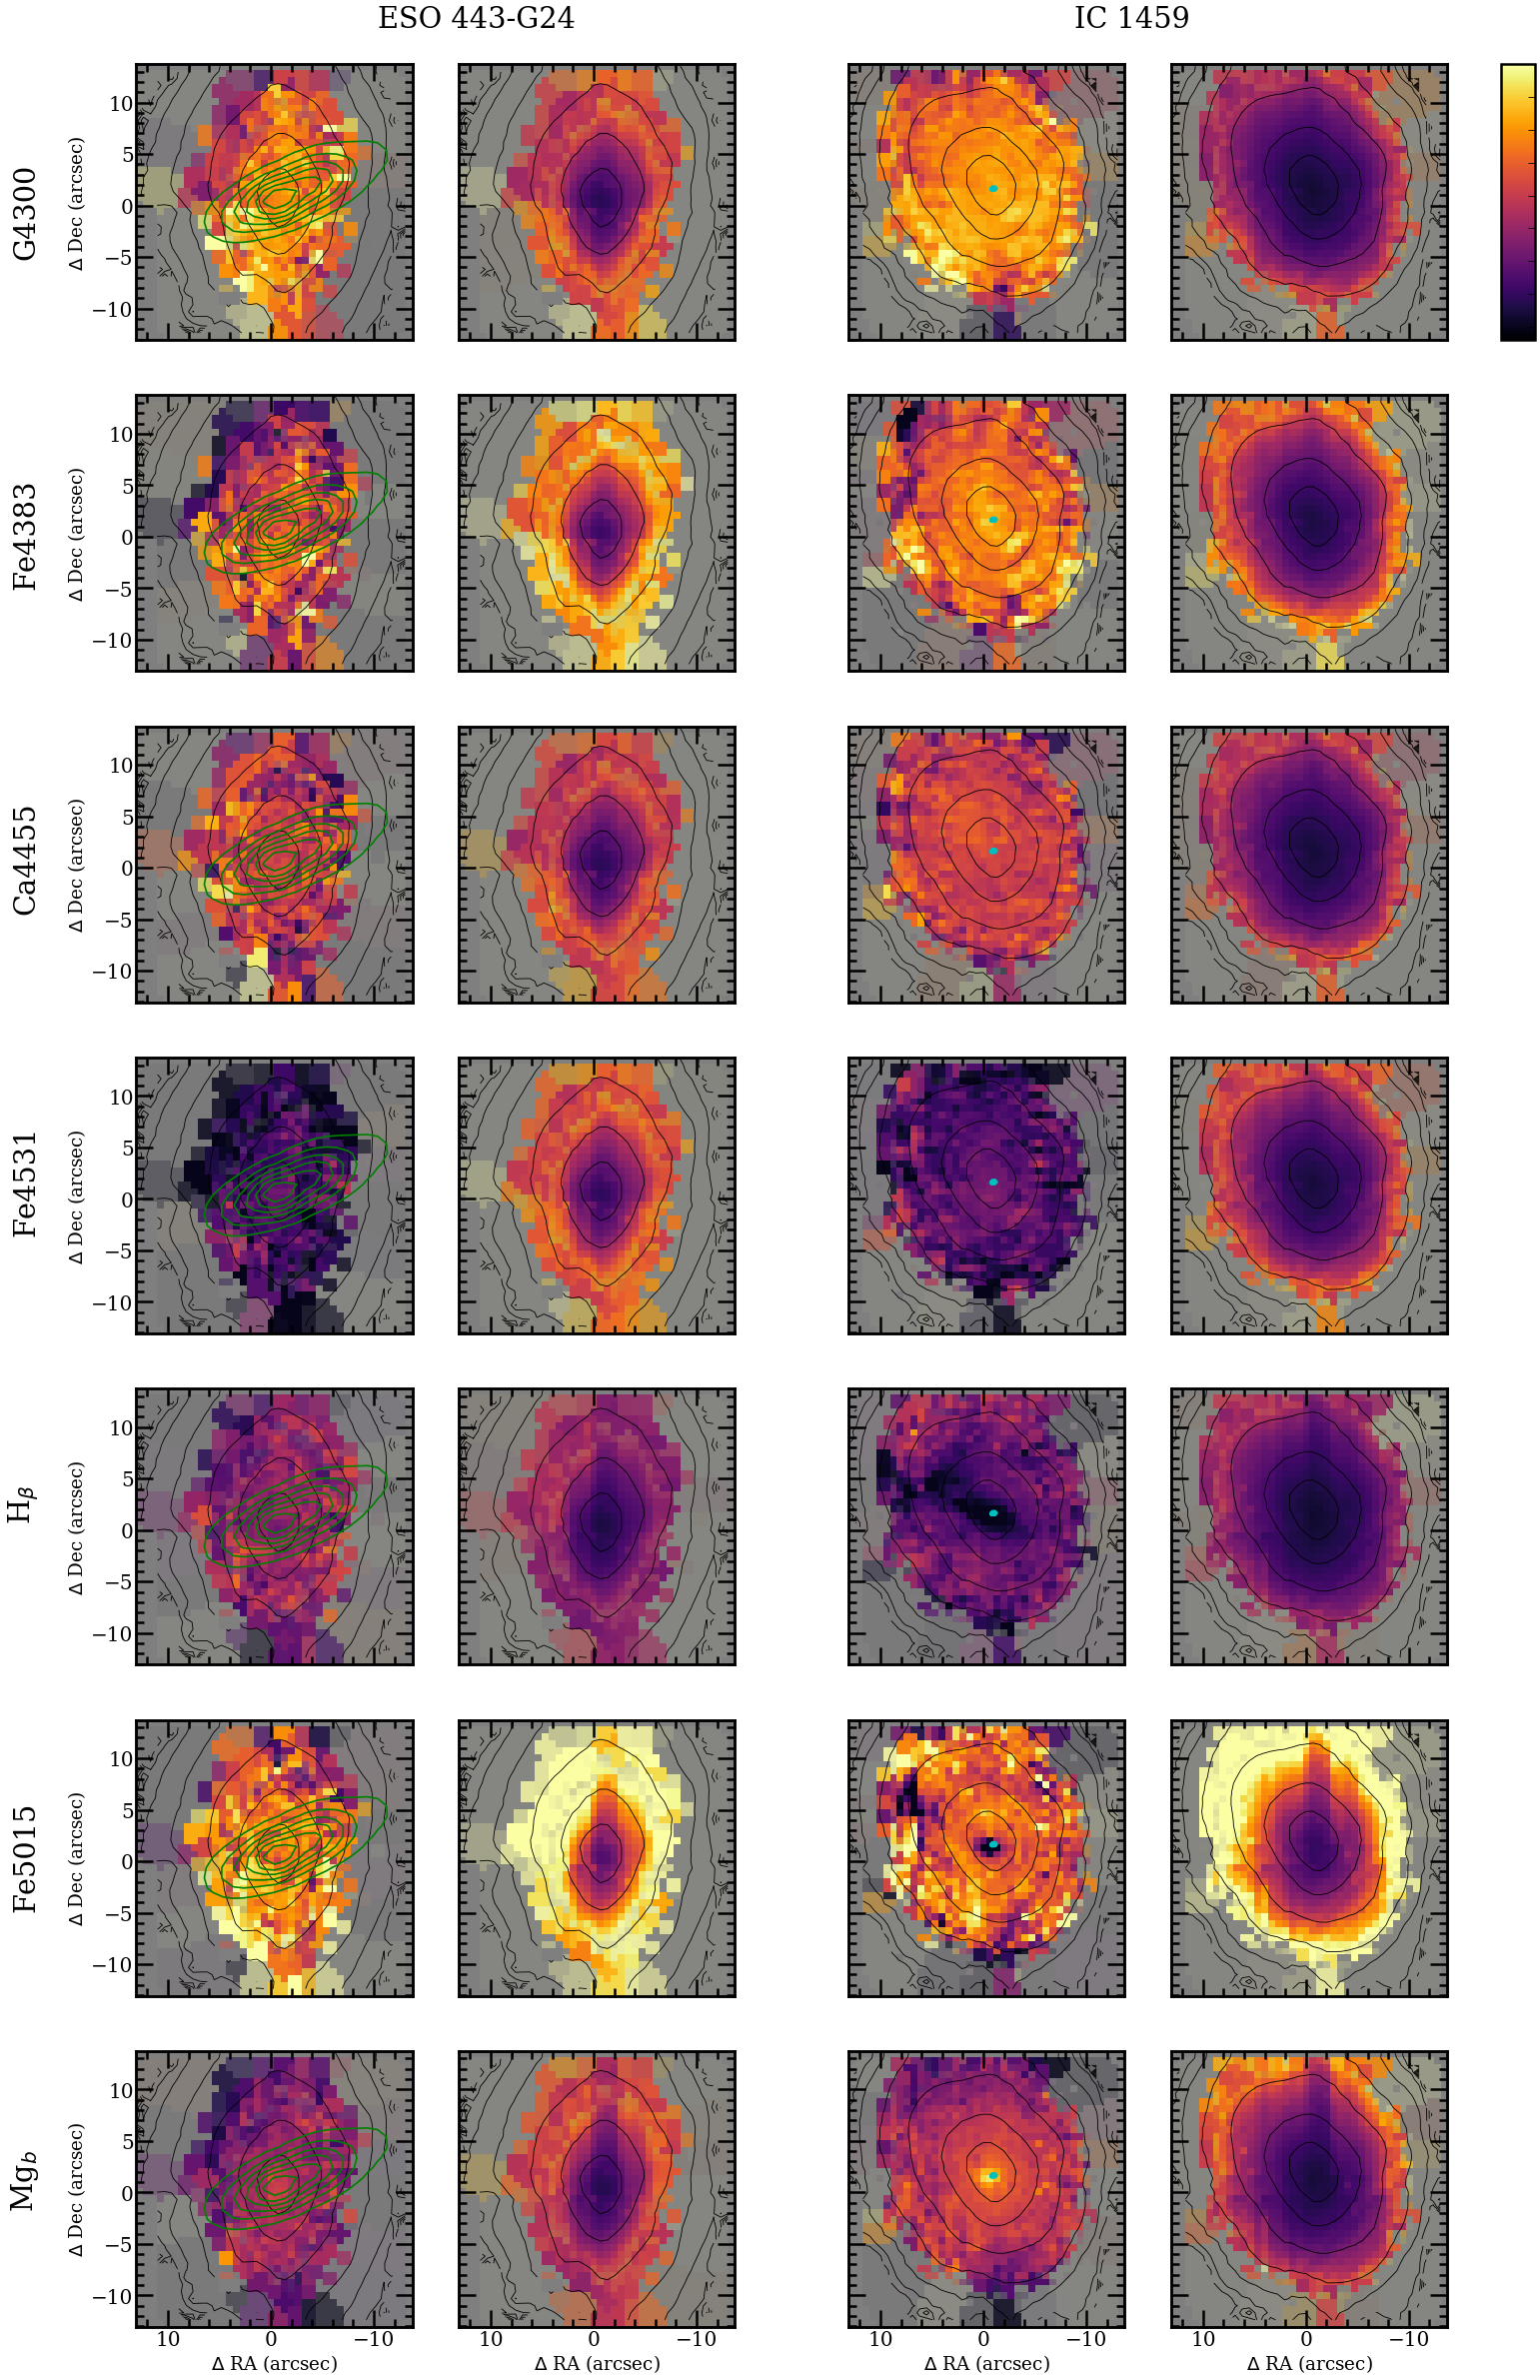
\includegraphics[height=0.89\textheight]{chapter4/vimos/abs1.png}
			\caption[VIMOS absorption line strength maps]{VIMOS absorption line strength maps. Left to right: ESO 443-G24 line index and associated uncertainties, IC 1459 line index and associated uncertainties. Top to bottom: G4300, Fe4383, Ca4455, Fe4531, H\,$\beta$, Fe5015 and Mg\,b index. Contours are as in Fig.\,\ref{fig:VIMOS_stellar}. Limits on the colour scales are 0.5--3.5\,\AA\ for Ca4455 and H\,$\beta$ line strengths, 3--7\,\AA\ for all other line strengths and 0--0.5\,\AA\ for all uncertainty maps.}
			\label{fig:VIMOS_absorption}
		\end{figure}
		\begin{figure}
			\centering
			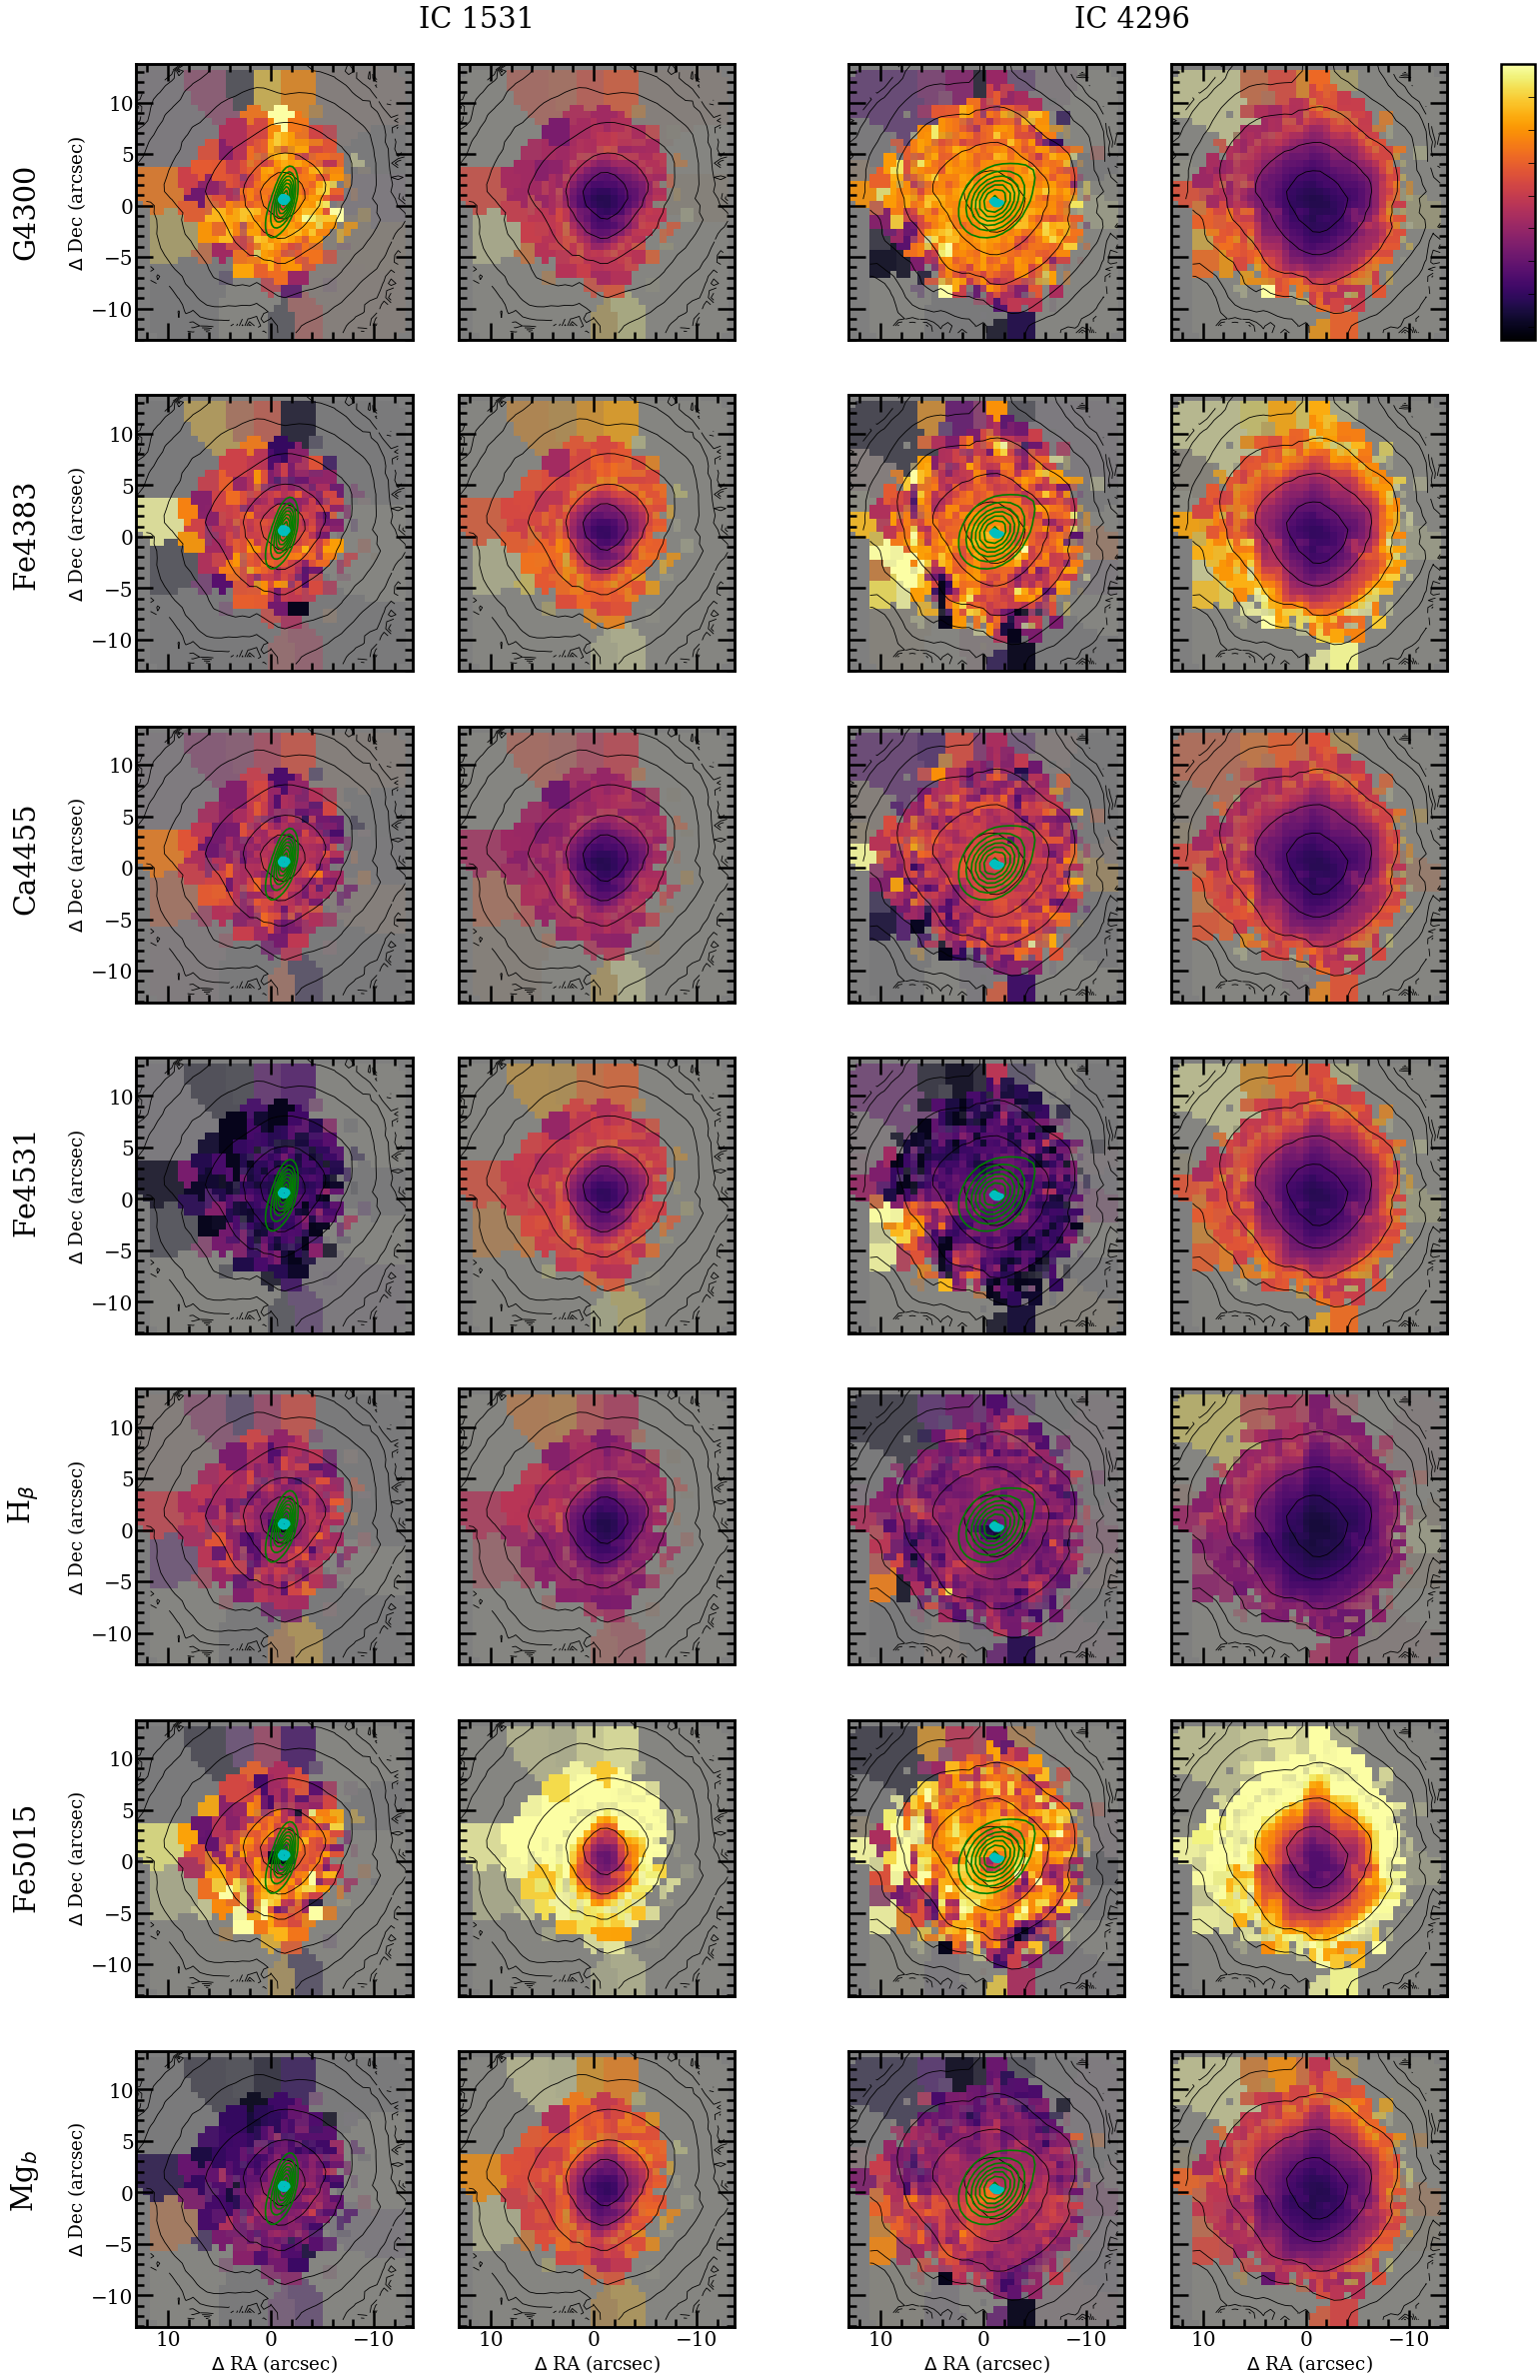
\includegraphics[height=0.94\textheight]{chapter4/vimos/abs2.png}
			\contcaption{\textit{Continued.}}% for IC 1531 and IC 4296.}
		\end{figure}
		\begin{figure}
			\centering
			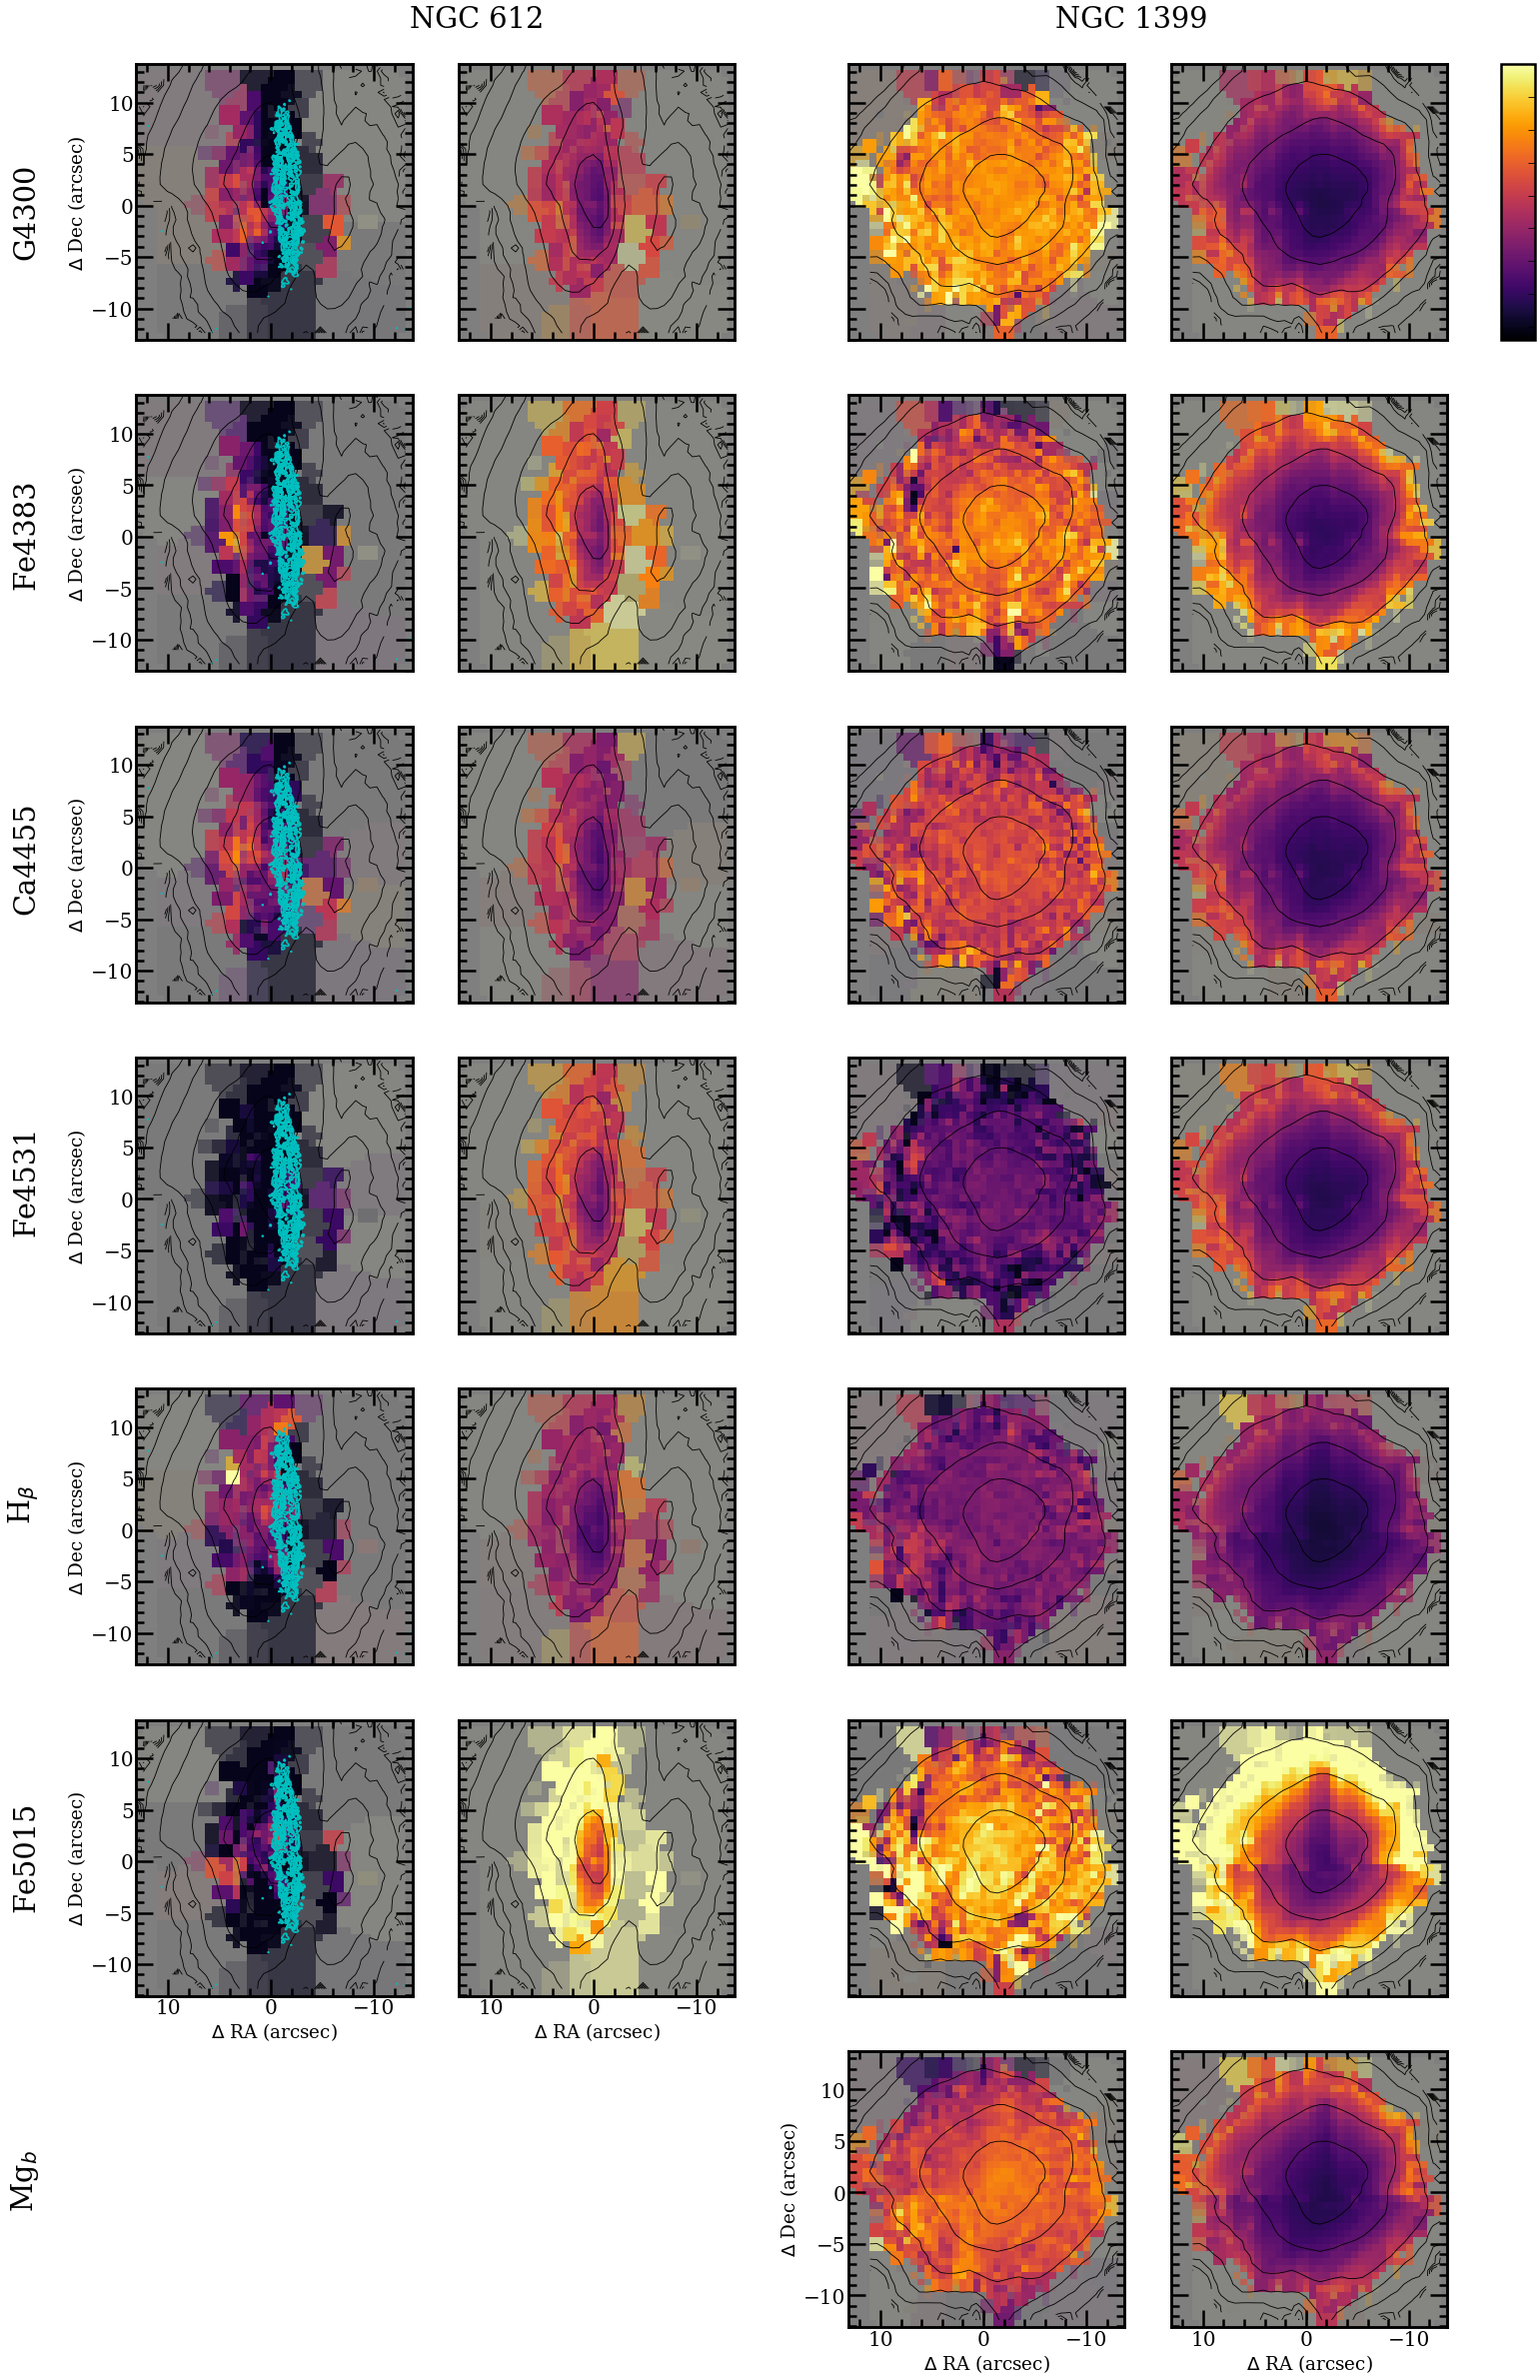
\includegraphics[height=0.94\textheight]{chapter4/vimos/abs3.png}
			\contcaption{\textit{Continued.}}% for NGC 612 and NGC 1399}
		\end{figure}
		\begin{figure}
			\centering
			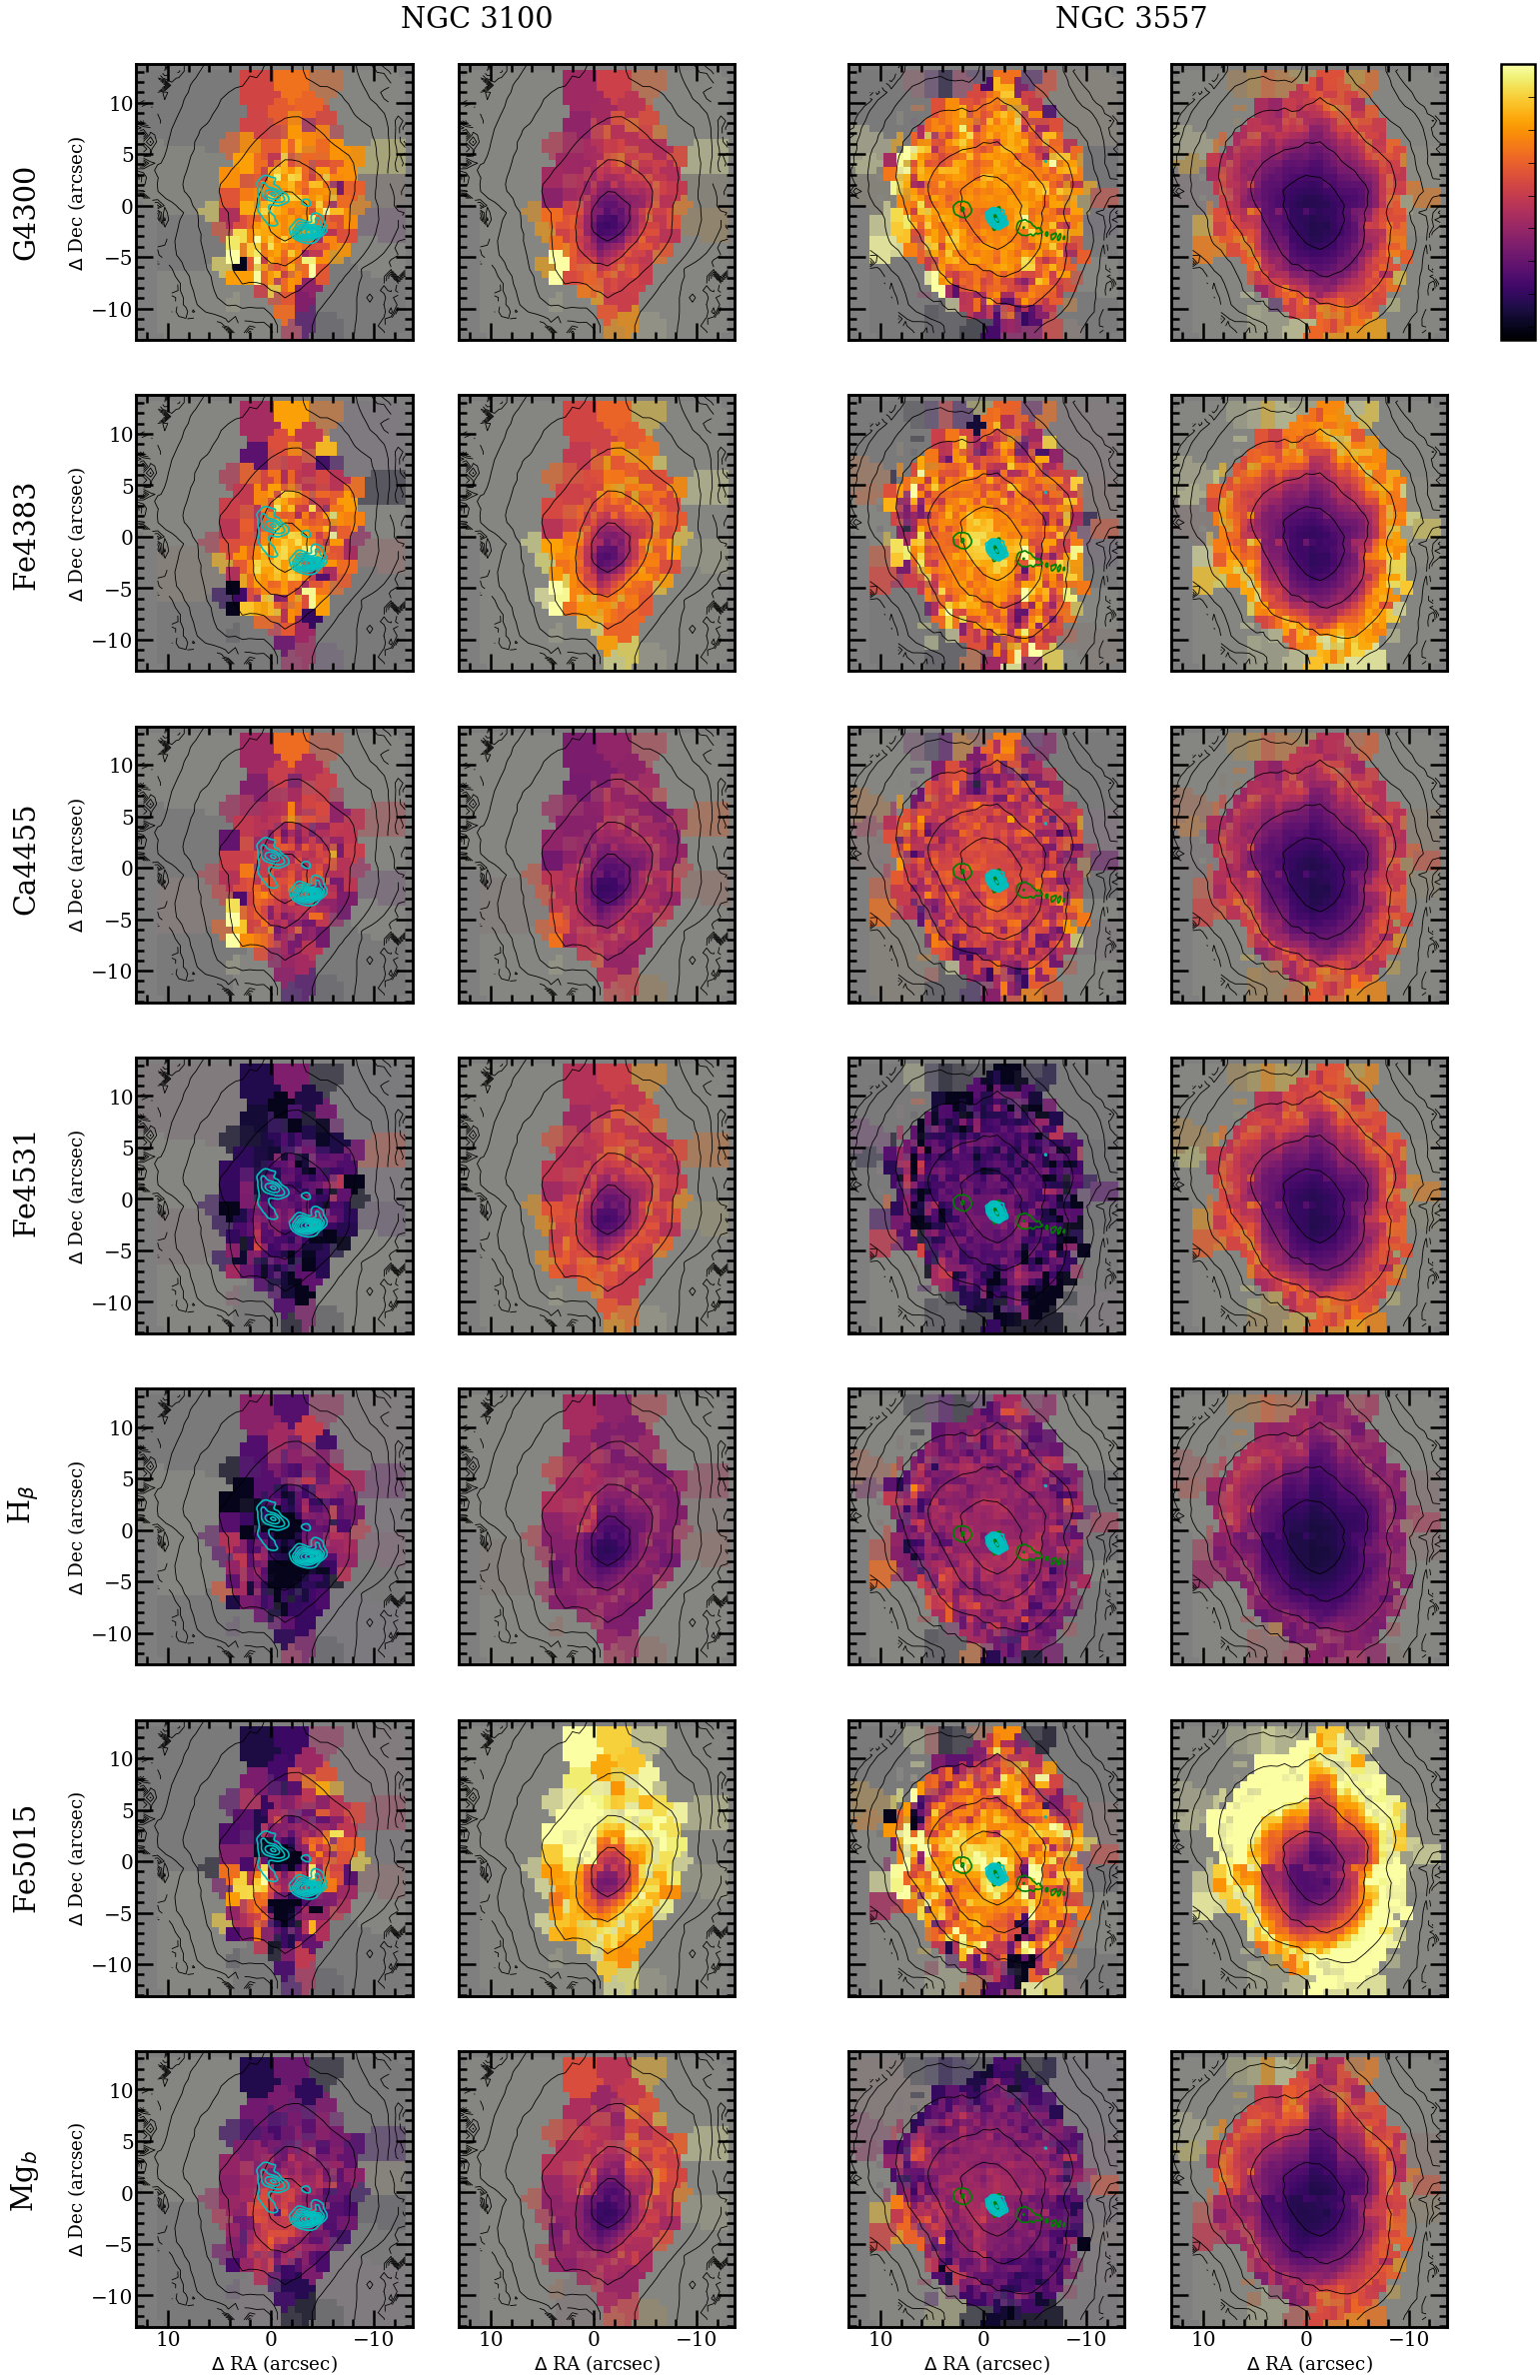
\includegraphics[height=0.94\textheight]{chapter4/vimos/abs4.png}
			\contcaption{\textit{Continued.}}% for NGC 3100 and NGC 3557}
		\end{figure}
		\begin{figure}
			\centering
			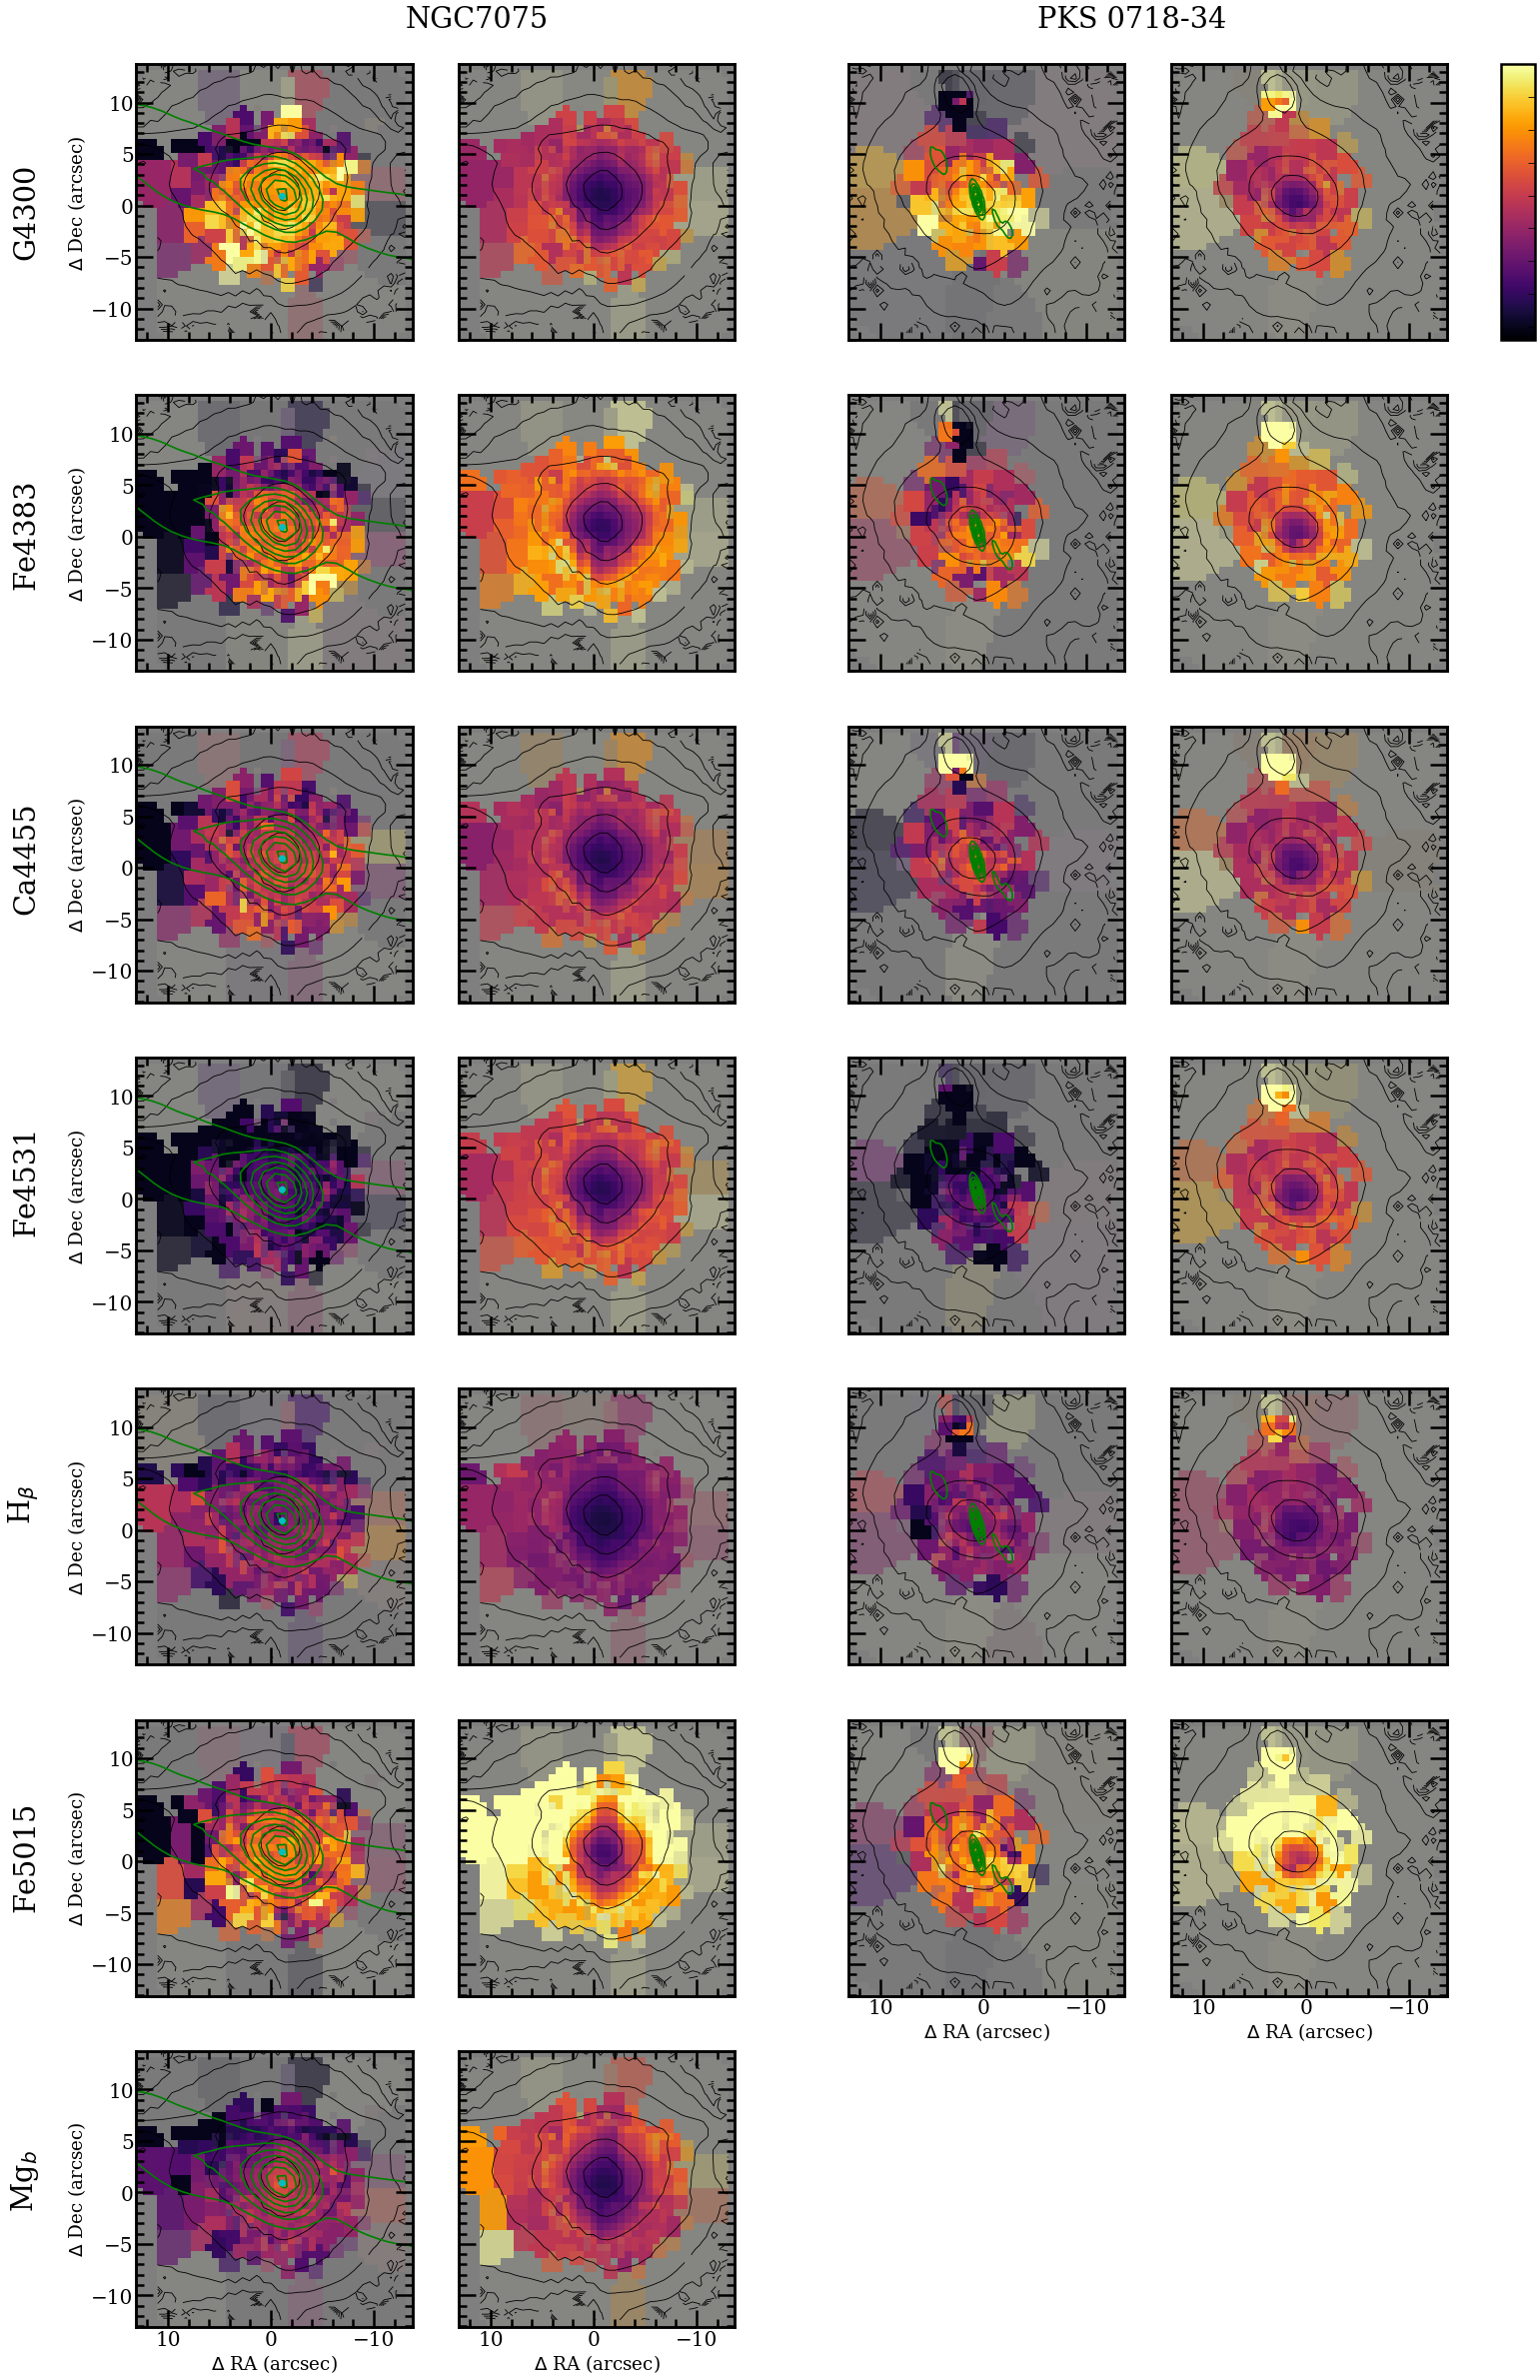
\includegraphics[height=0.94\textheight]{chapter4/vimos/abs5.png}
			\contcaption{\textit{Continued.}}% for NGC 7075 and PKS 718-34}
		\end{figure}

		\begin{figure}
			\centering
			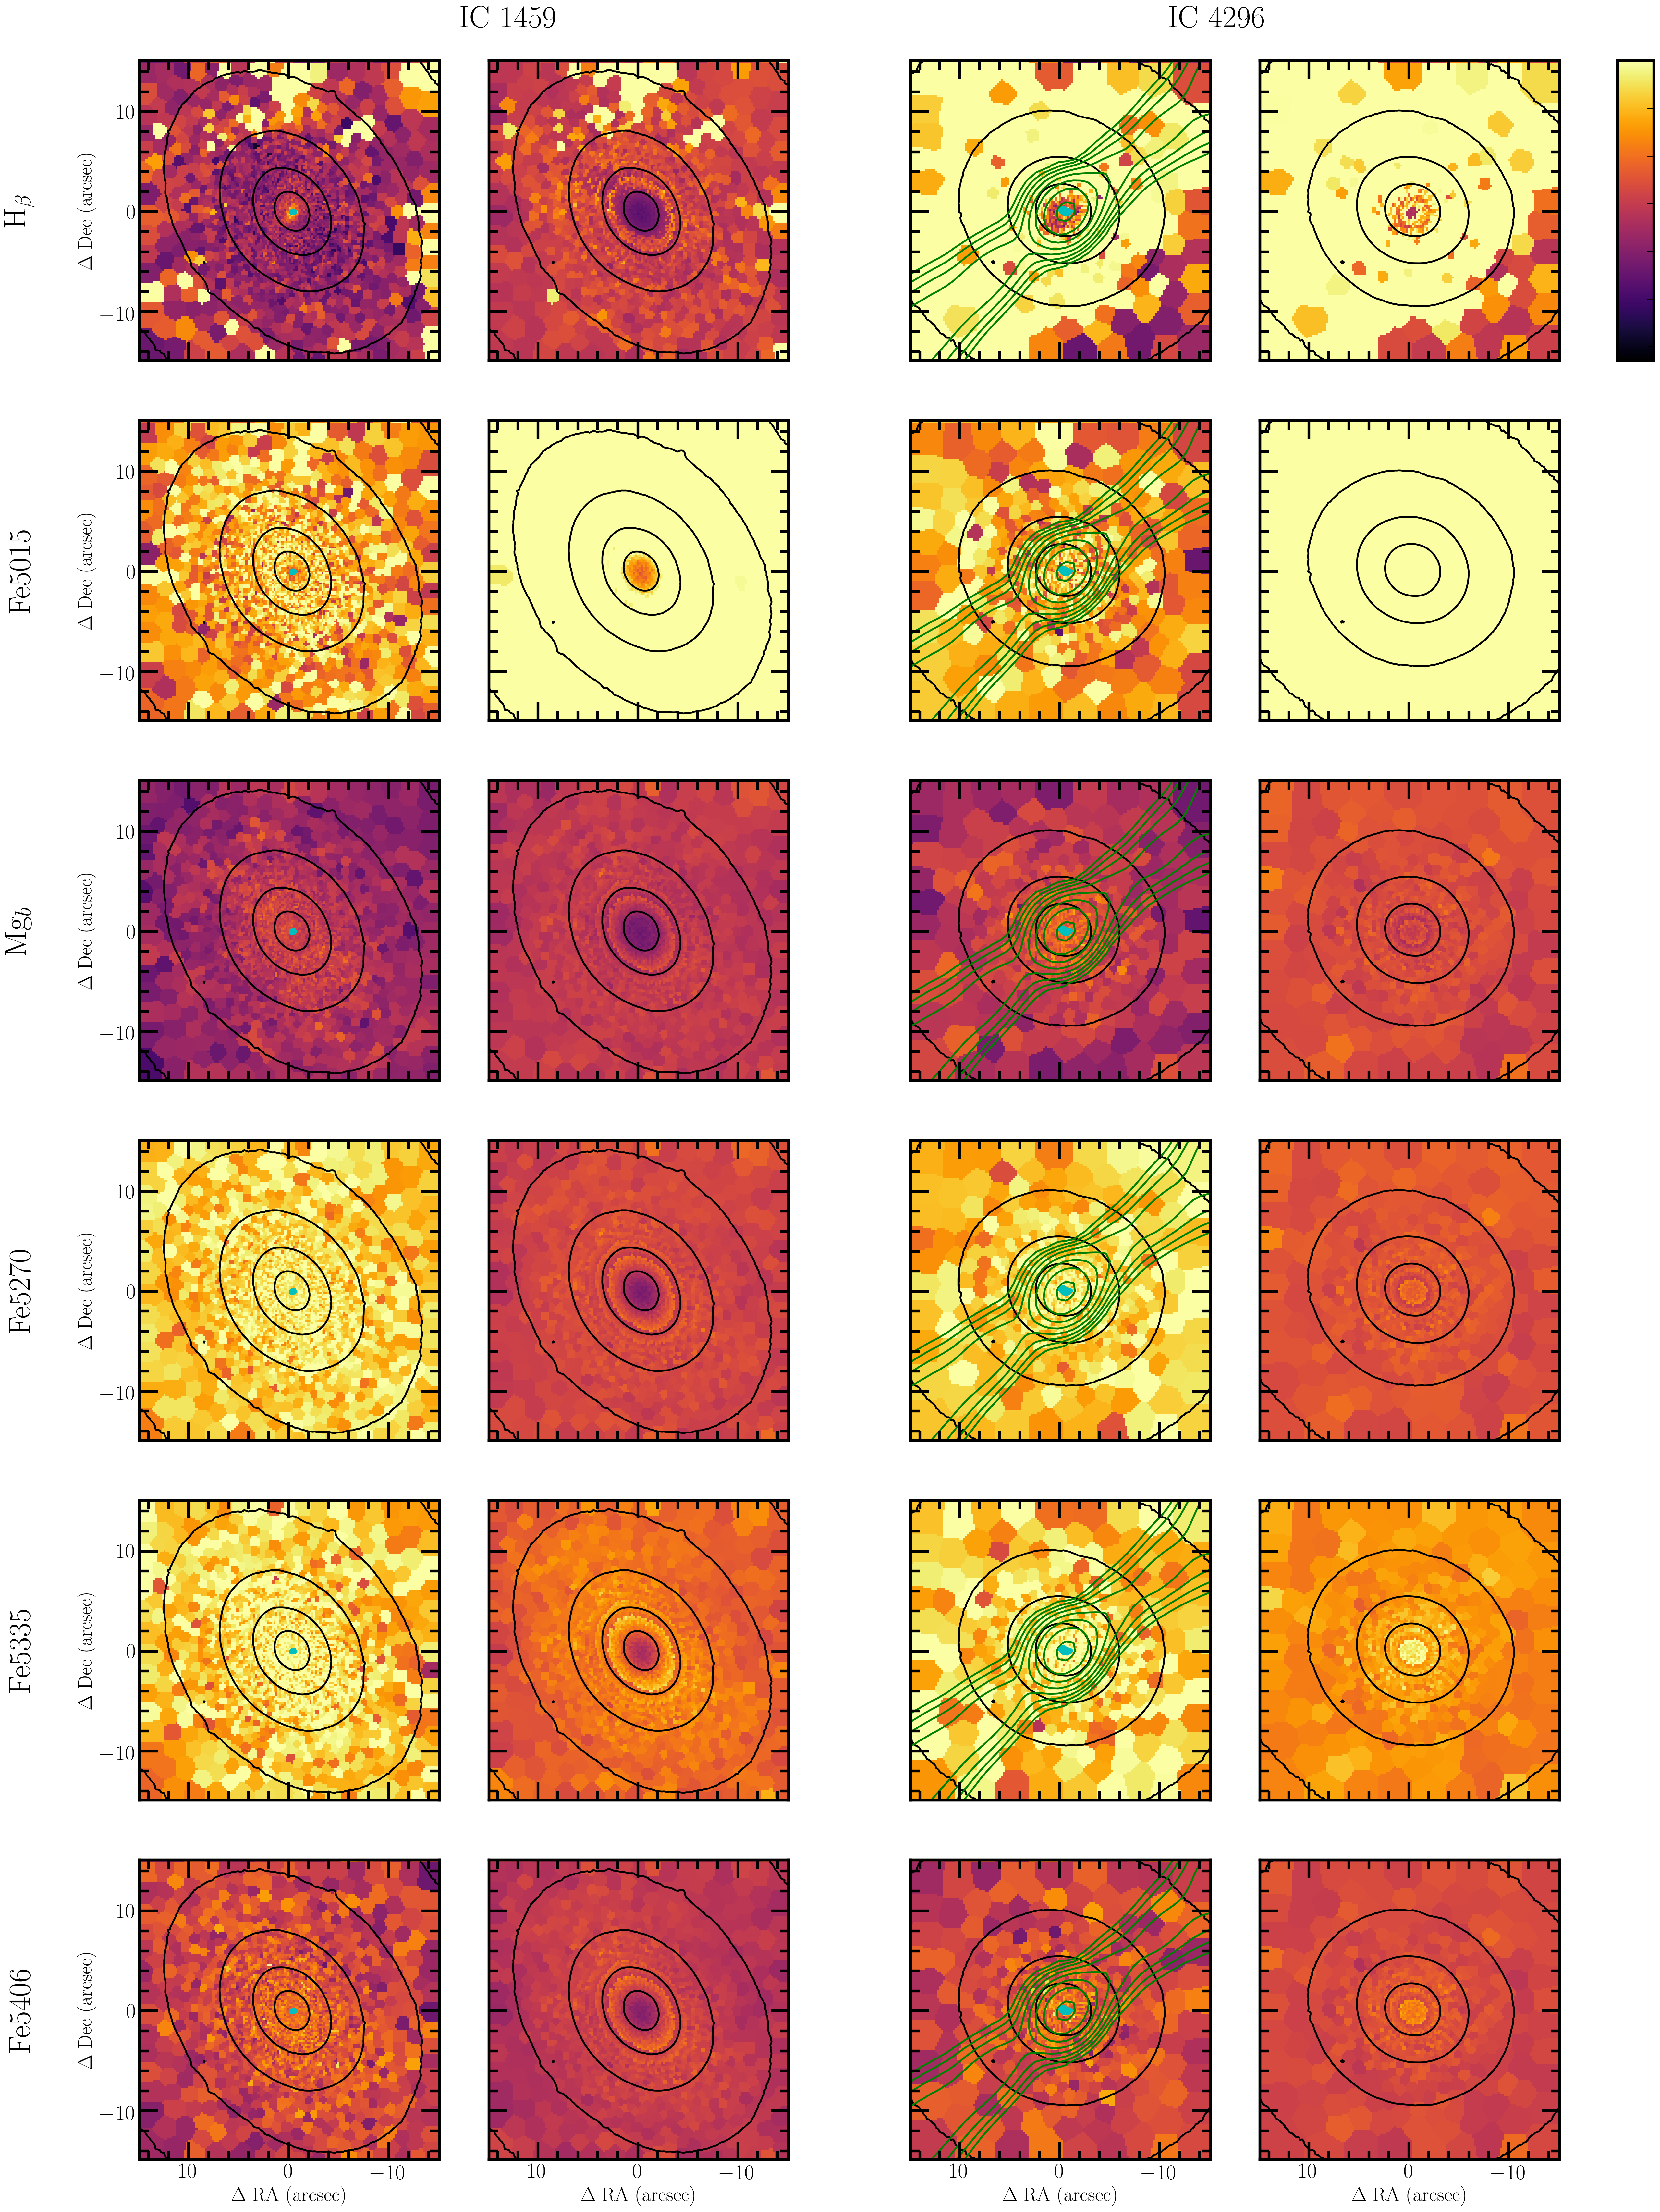
\includegraphics[height=0.81\textheight]{chapter4/muse/abs1.png}
			\caption[MUSE absorption line strength maps]{As Fig.\,\ref{fig:VIMOS_absorption} but for the MUSE absorption line strength maps. Limits on the colour scales are 0.5--3.5\,\AA\ for the H\,$\beta$, Fe5270, Fe 5335, Fe5406, Fe5709 and Fe5782 indices, 0--0.35\,mag for the TiO1 index, 0--0.1\,mag for the TiO2 index and 3--7\,\AA\ for all other indices. For the uncertainty maps the colour scale limits are 0--0.03\,mag for the TiO1 and TiO2 indices and 0--0.5\,\AA\ for all other indices.}
			\label{fig:MUSE_absorption}
		\end{figure}
		\begin{figure}
			\centering
			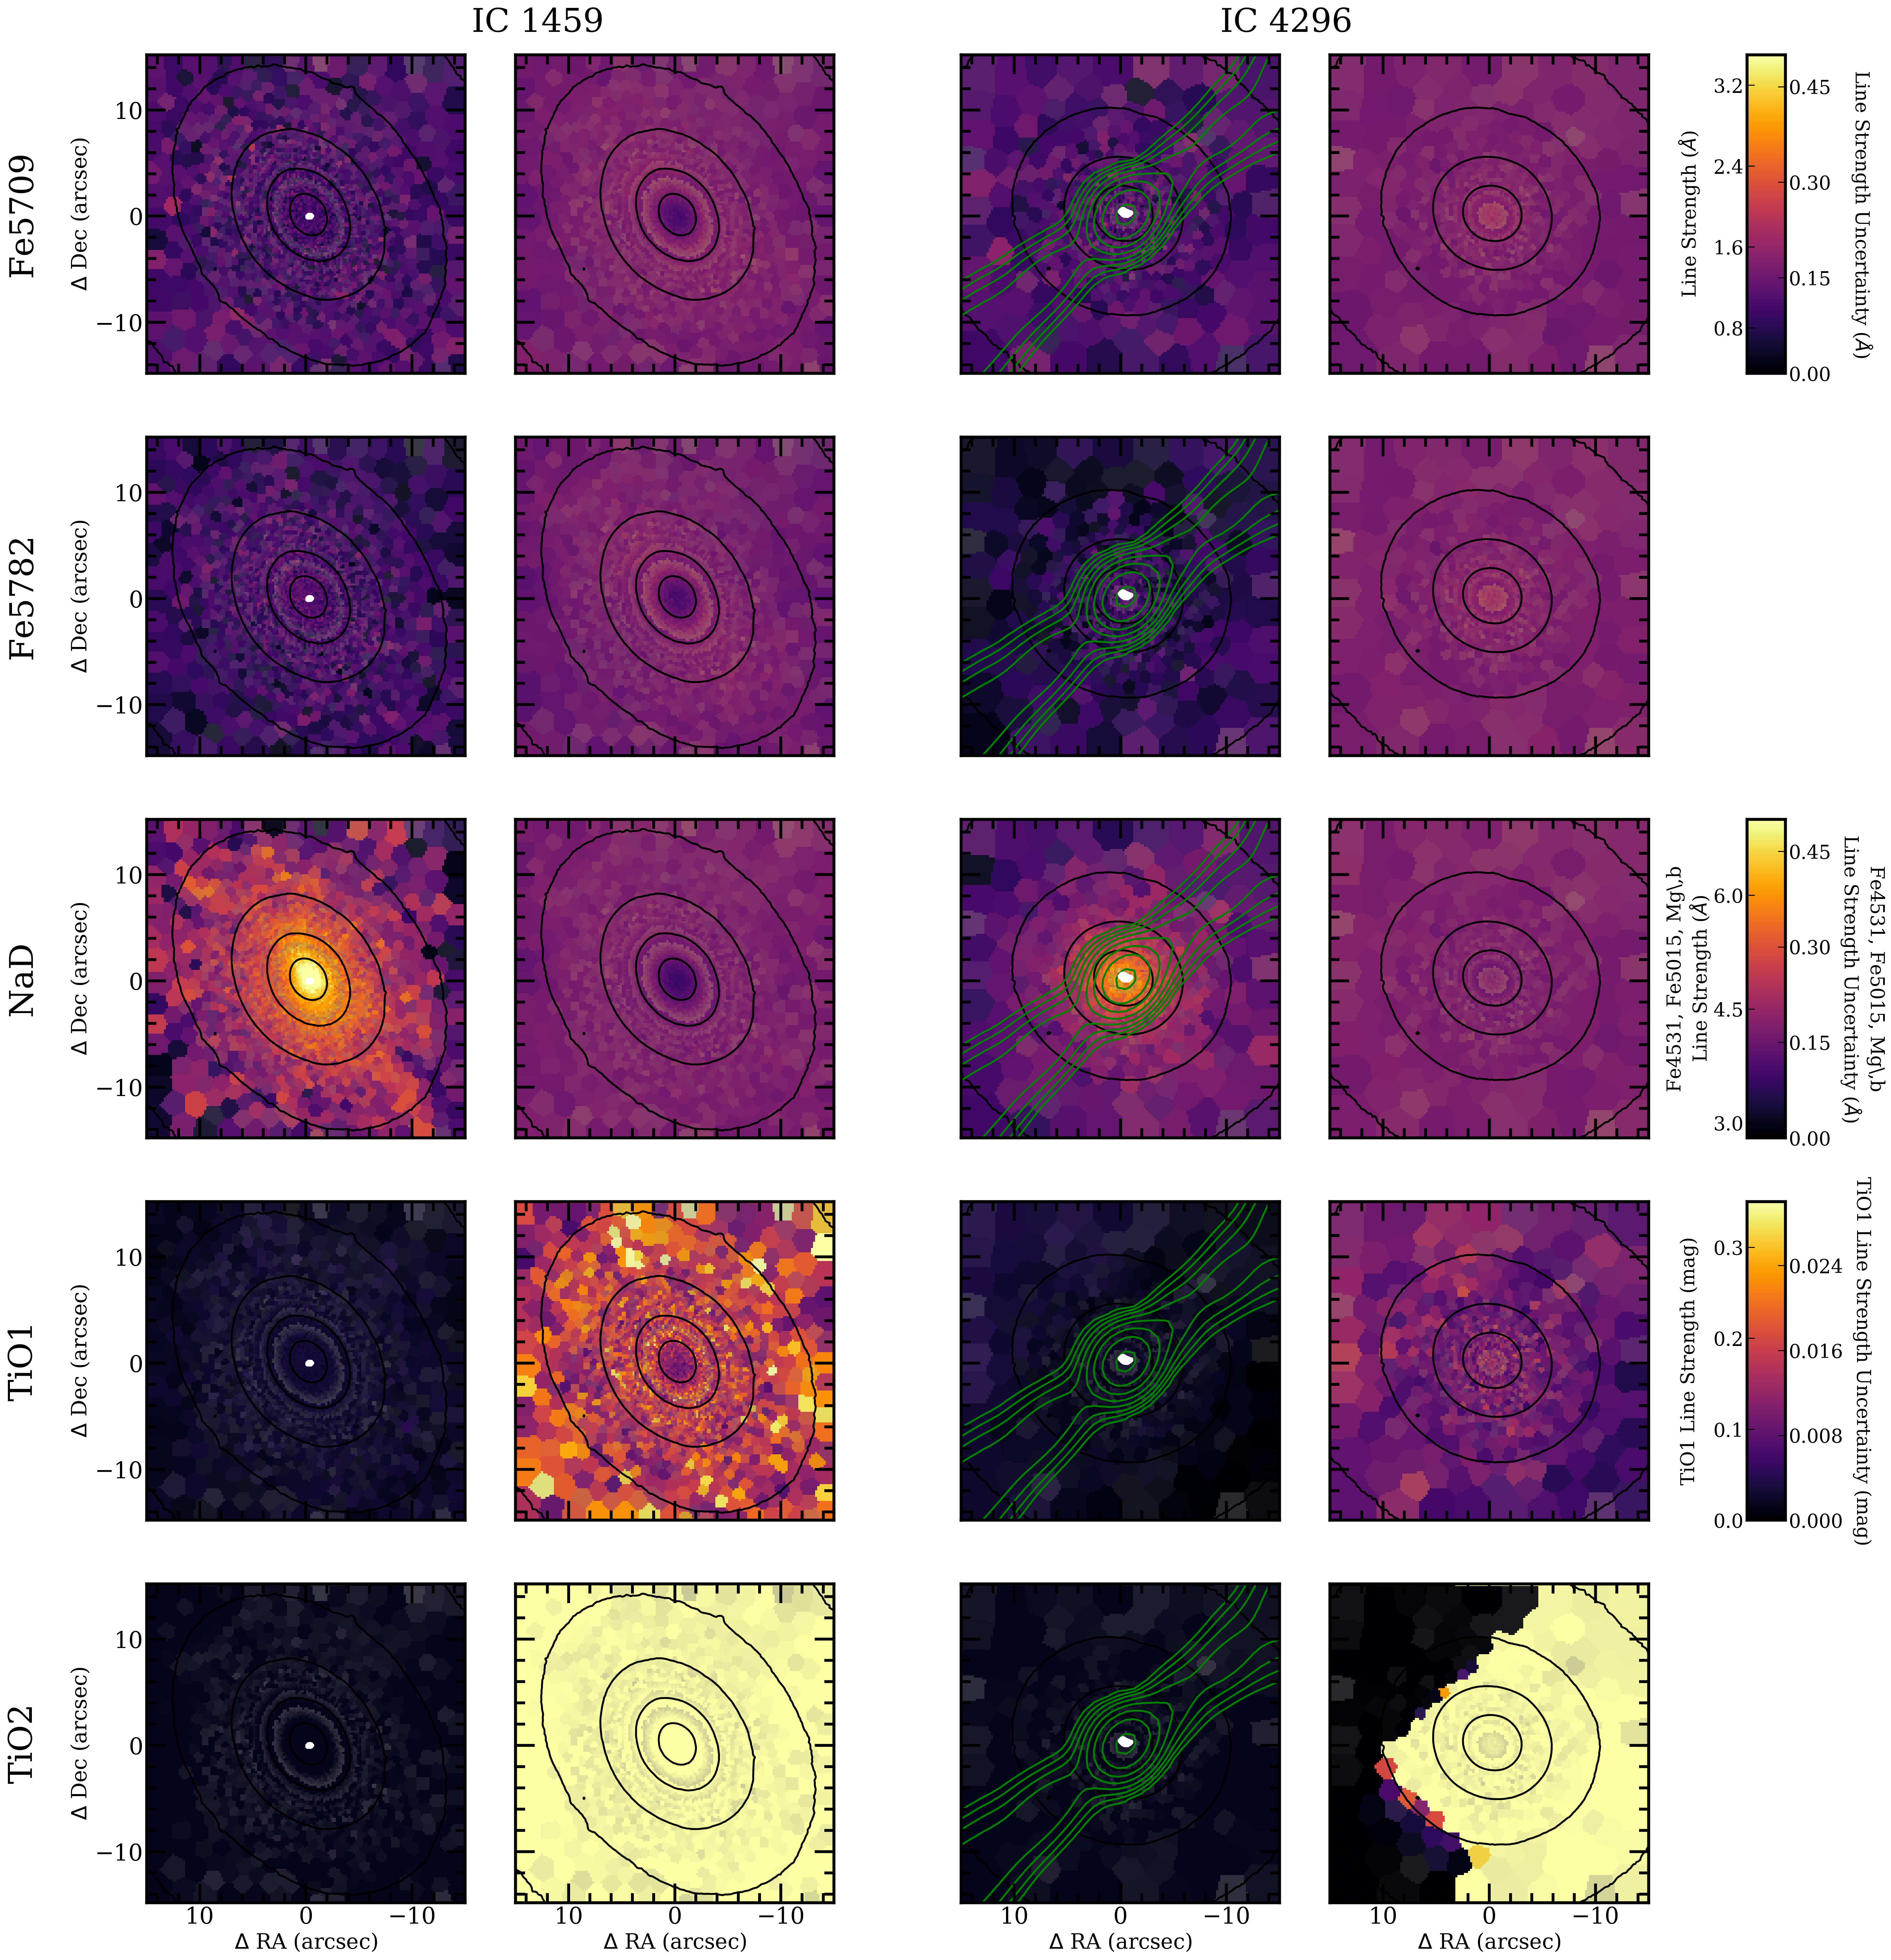
\includegraphics[height=0.67\textheight]{chapter4/muse/abs1b.png}
			\contcaption{\textit{Continued.}} %: From top to bottom: Fe5782, NaD, TiO1, TiO2. Plots are as in \ref{fig:VIMOS_stellar}. Limits on the colour scale are 0-9 \AA\ for the line strengths and 0-1 \AA\  for the uncertainties and 0-0.35 mag for TiO1 and TiO2 line strengths and 0-0.03 mag for the uncertainty in TiO1 and TiO2.}
		\end{figure}
		\begin{figure}
			\centering
			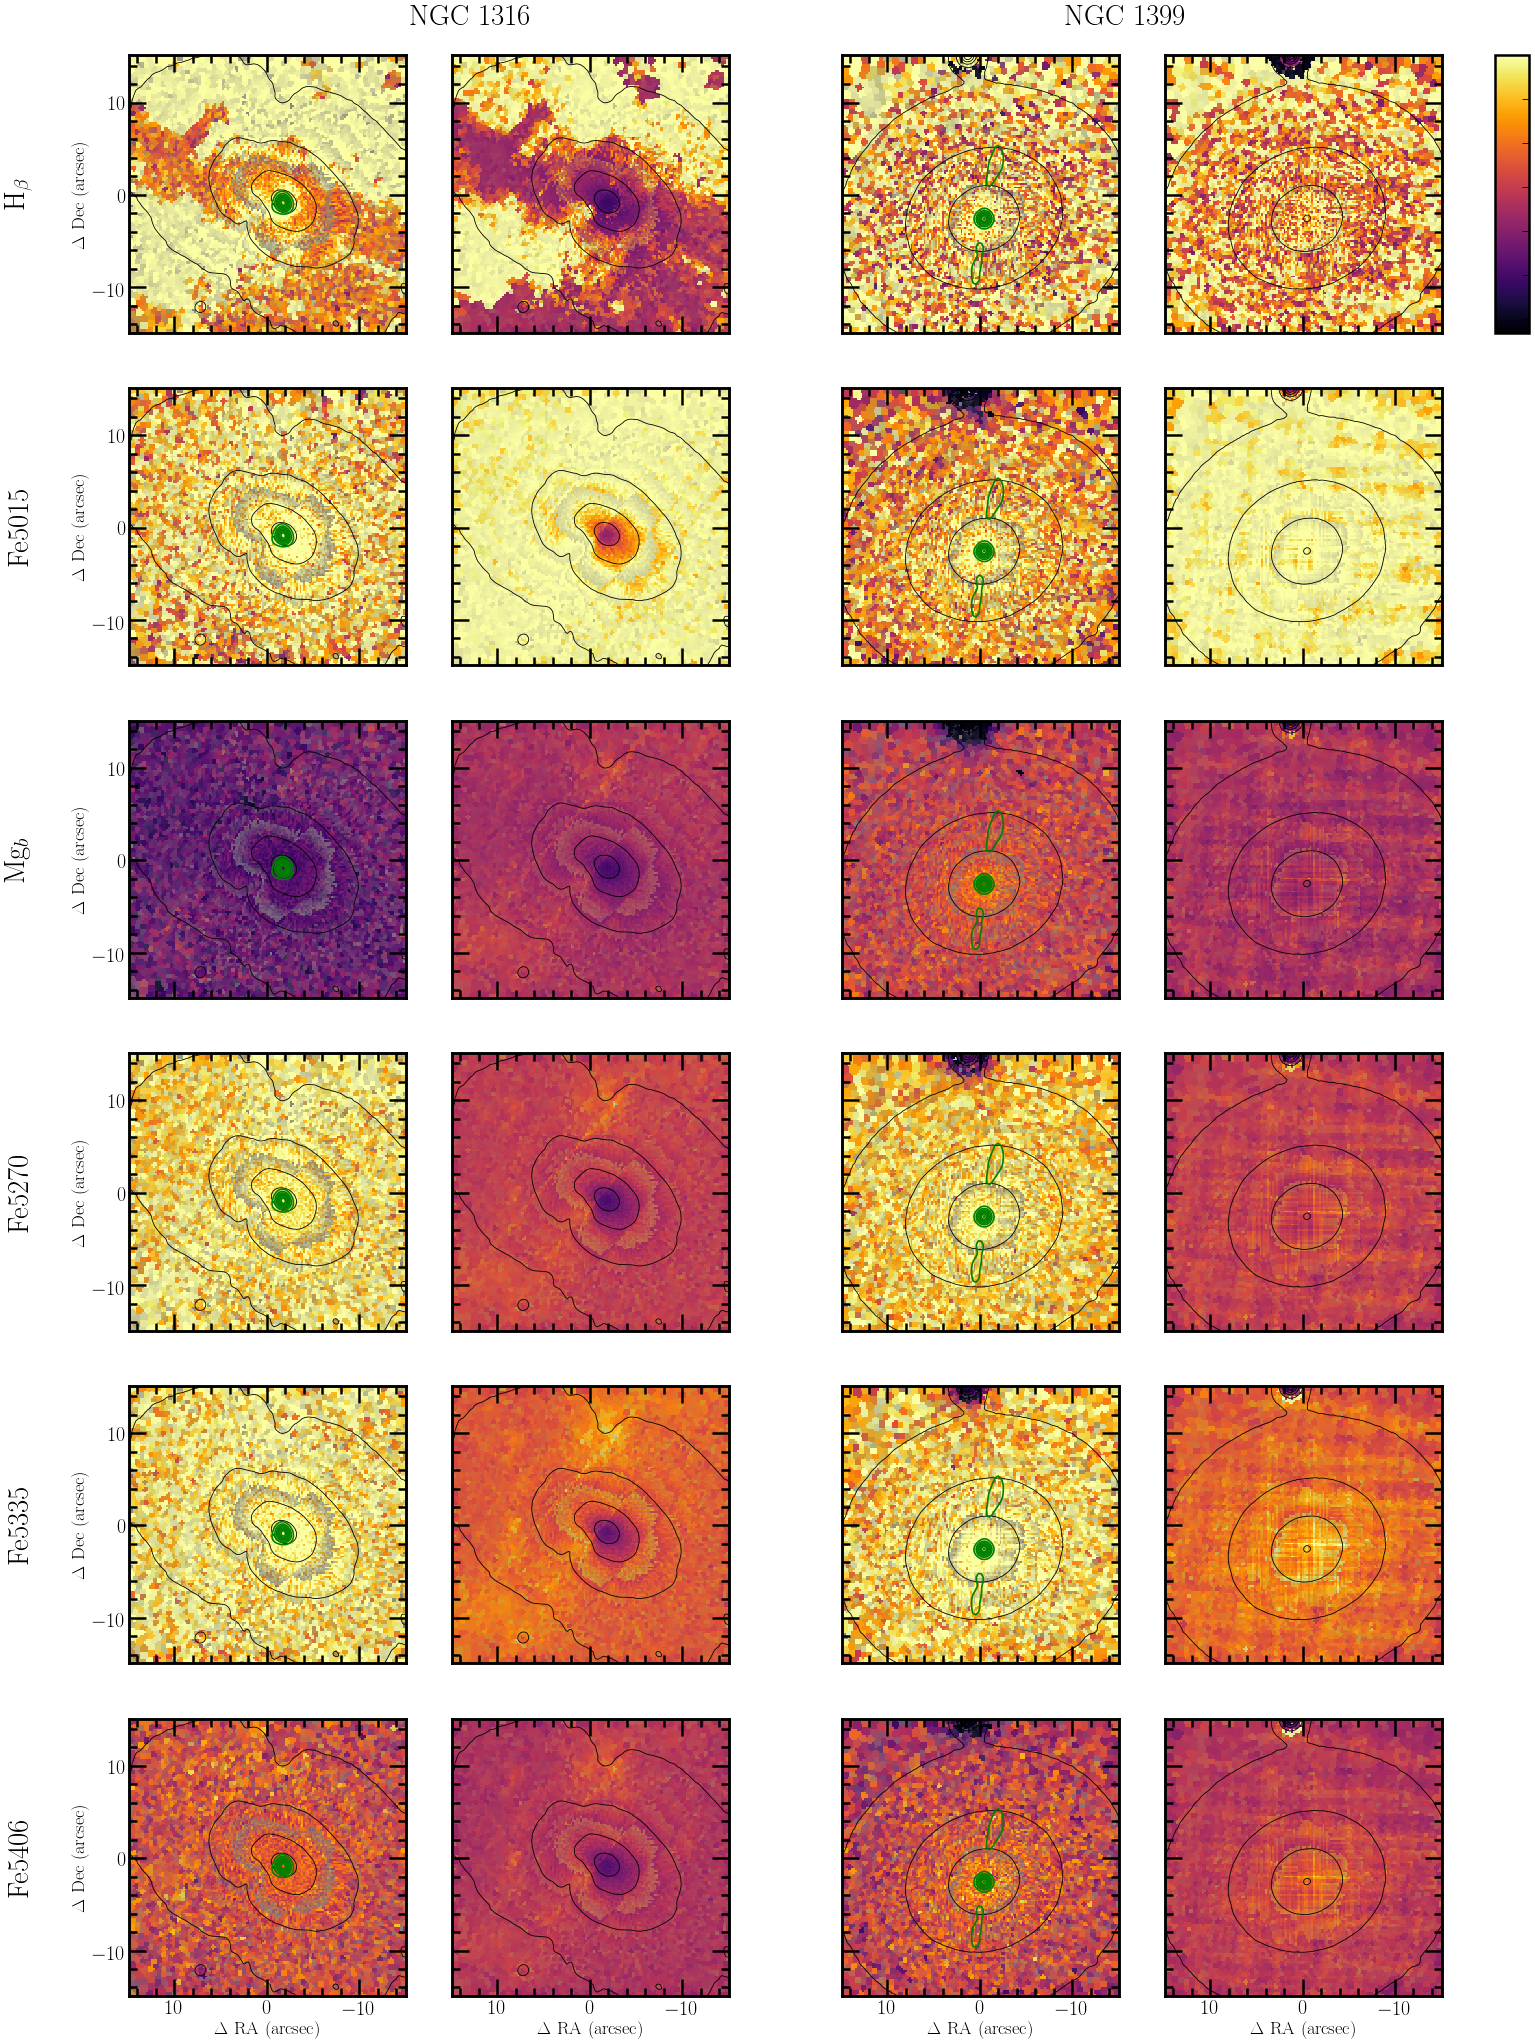
\includegraphics[height=0.81\textheight]{chapter4/muse/abs2.png}
			\contcaption{\textit{Continued.}}% for NGC1316 and NGC1399.}
		\end{figure}
		\begin{figure}
			\centering
			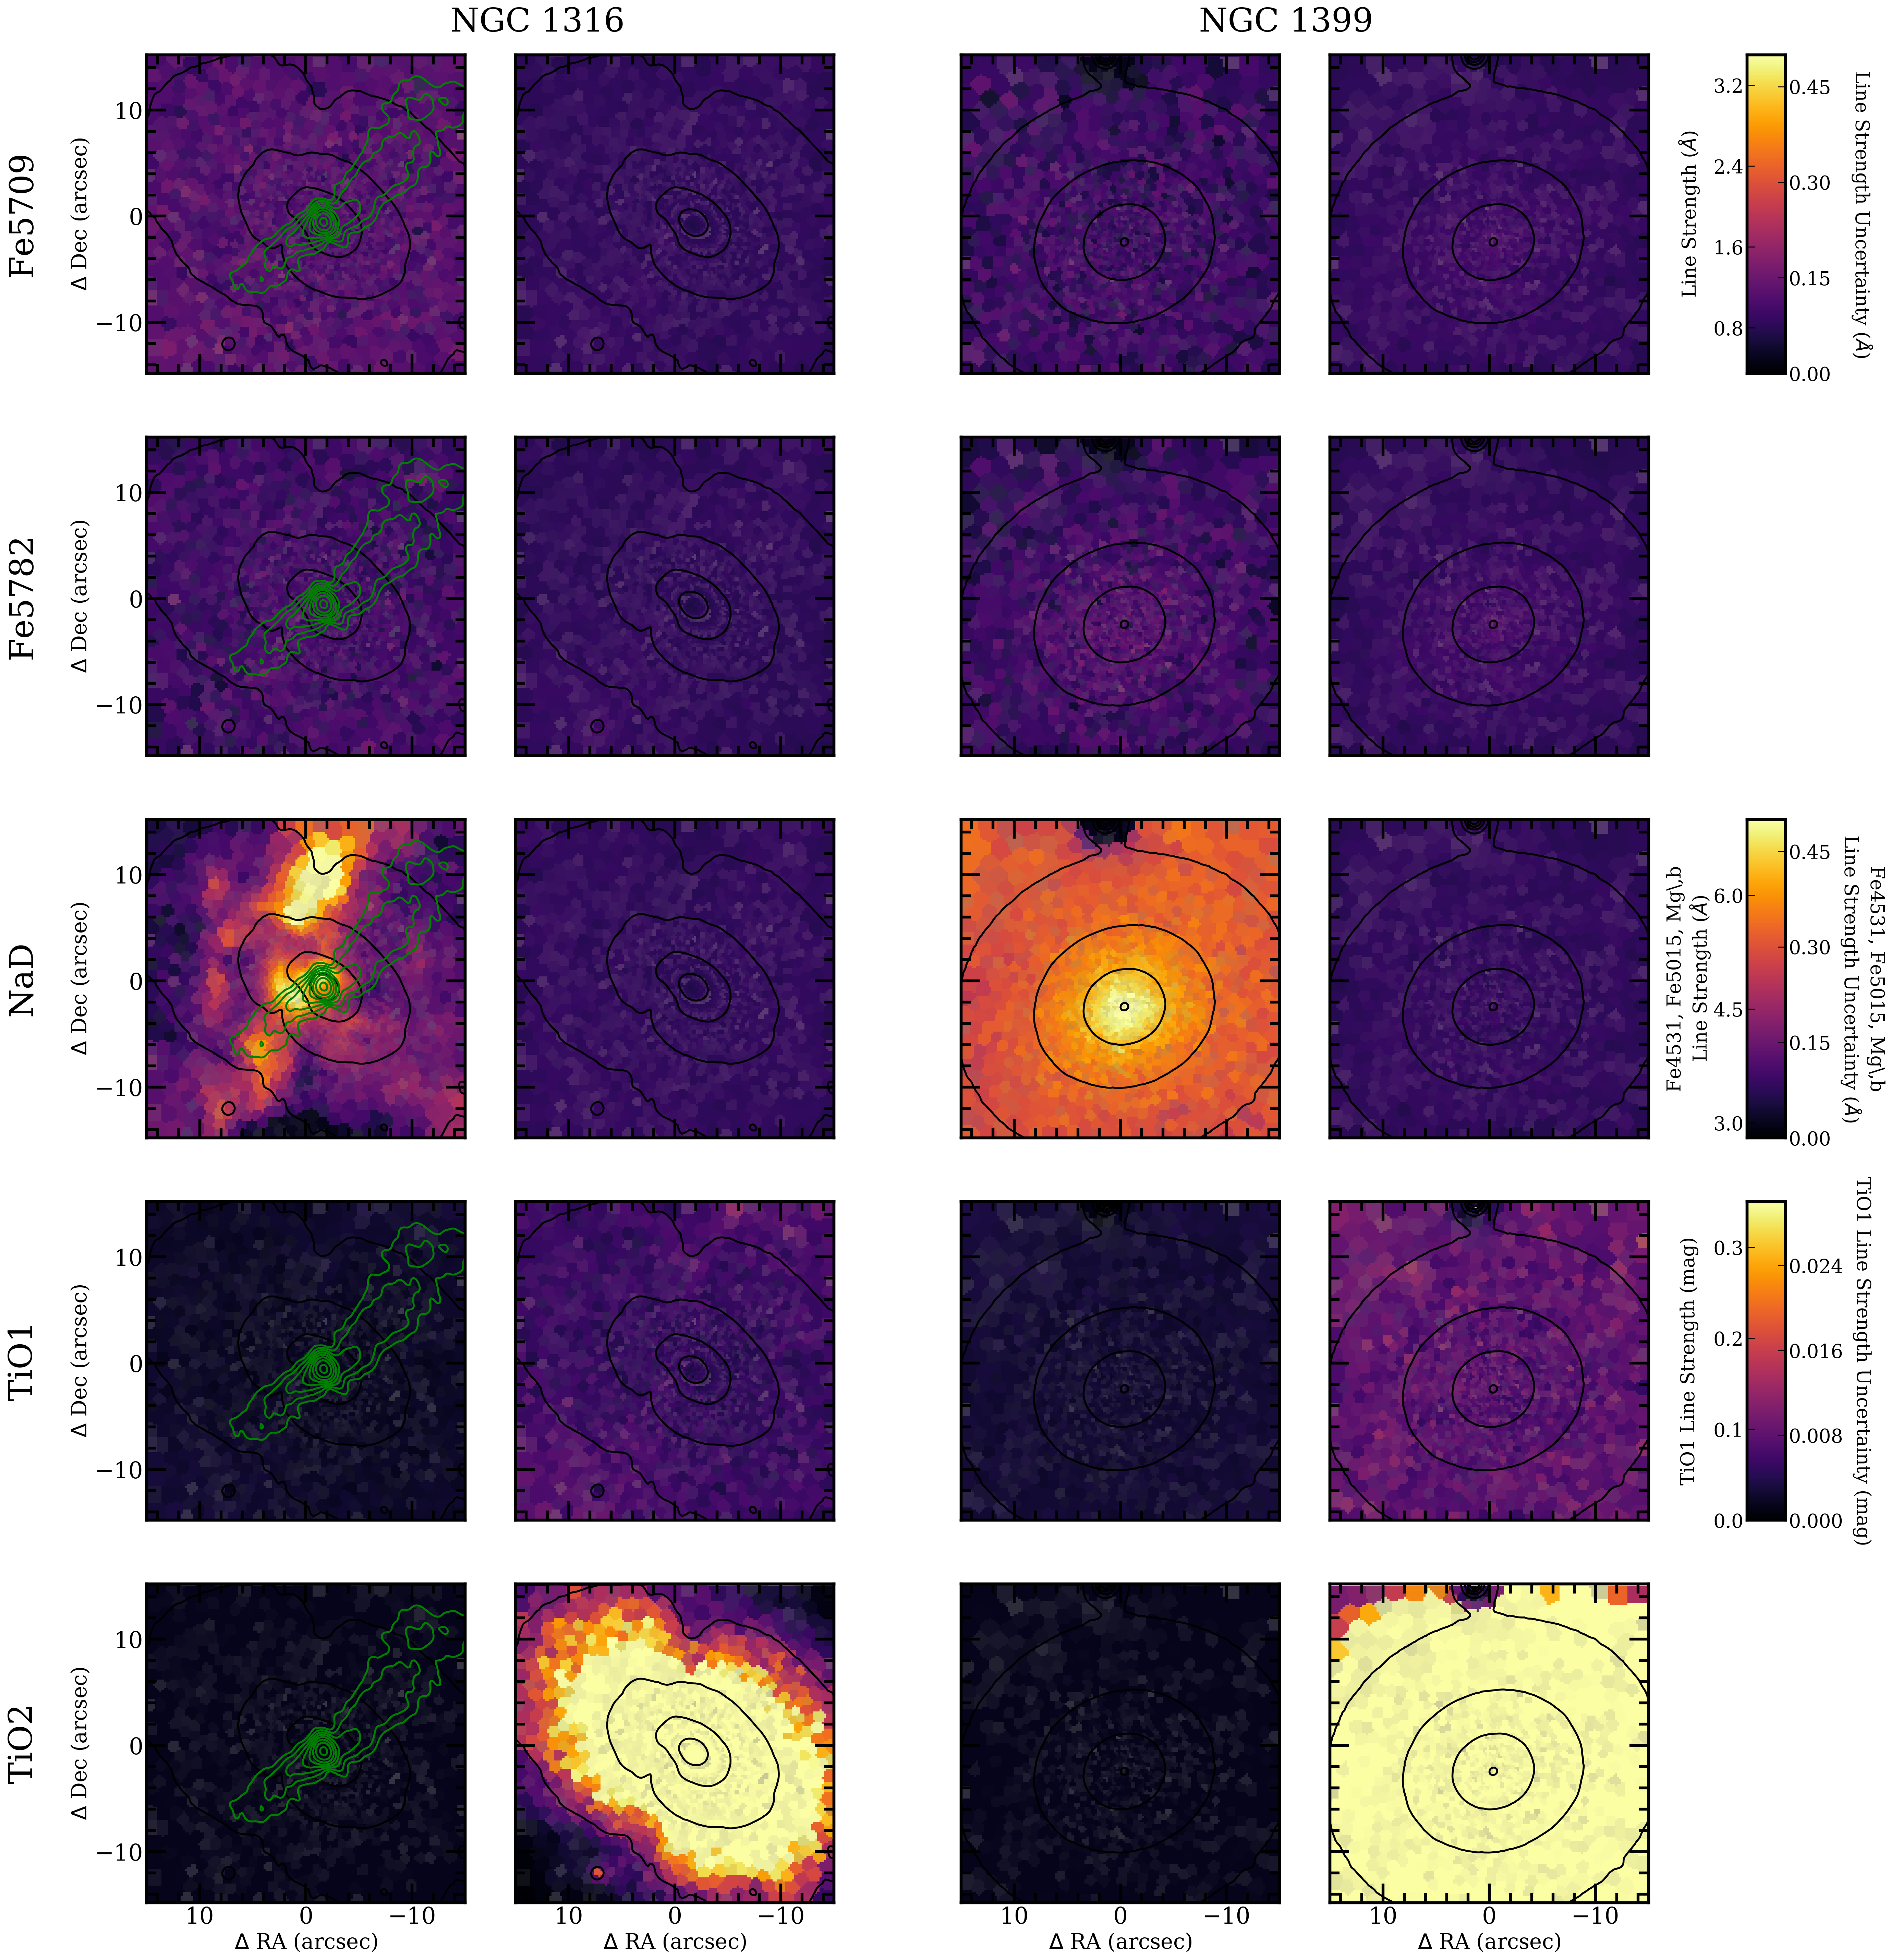
\includegraphics[height=0.67\textheight]{chapter4/muse/abs2b.png}
			\contcaption{\textit{Continued.}}% for NGC1316 and NGC1399.}
		\end{figure}

			We observe that most of our Southern sample show almost uniform, small H\,$\beta$ line strengths throughout a given galaxy, as well as slight central concentration in Fe, Ca4455 and Mg\,b index maps. NGC 612 is the exception to these trends, with large H\,$\beta$ line strengths, particularly along the dust lane and larger gradients in Fe and Ca4455 (see description in Appendix \ref{cha:Description}). The MUSE derived maps also show significant central concentration in the NaD index. The NaD feature is thought to be significantly deepened by absorption from the interstellar medium (ISM), if present \citep[e.g.][]{Phillips1993, Bergmann2009}, a concept consistent with the NaD line strength map of NGC 1316 where the strongest absorption is seen in the dust lane. Like NGC 612, NGC 1316 also has large H\,$\beta$ line strengths, again with the highest values along the dust lane. 

		\subsubsection{Mg -- $\sigma$ relation}
			\label{subsubssec:Mgsigma}
			The definition of the Mg$_2$ absorption line index (blue continuum: 4895.125--4957.625\,\AA, index bandpass: 5154.125--5196.625\,\AA\ and red continuum: 5301.125--5366.125\,\AA) has overlapping bandpasses with the Mg\,b index, but includes the MgH molecular absorption line, and is hence considered a molecular index and is measured in units of magnitude. \citet{Bender1993} first noticed the unusually tight relationship between the global Mg$_2$ absorption line strength and logarithm of the central velocity dispersion, $\sigma_0$, in elliptical galaxies. They also noticed that residuals to the linear best-fit appeared to be intrinsic as they have a near Gaussian shape about the median values, but do not seem to be correlated to any other galaxy property. 

			Since part of the red continuum band of the Mg$_2$ index is outside of the spectral range of VIMOS, we instead use the Mg\,b index. \citet{Ziegler1997} show there is a linear relationship between Mg\,b and Mg$_2$, with a gradient of 14.3--15.5\,mag\,\AA$^{-1}$\ depending on metallicity. We thus use Mg\,b as a proxy for Mg$_2$. 

			Using an aperture with a radius of 2 arcsec on each datacube, we measure $\sigma_0$ and Mg\,b at a spectral resolution of 8.4\,\AA\ full-width half-maximum (FWHM; see Table \ref{tab:globalMg} and points in Fig.\,\ref{fig:globalMg}). The best-fitting linear relationship (found using \textsc{lts\_linefit} by \citealt{Cappellari2013}) has a gradient of $2.3 \pm 0.5 \,\mathrm{\AA\,dex^{-1}}$ (solid black line in Fig.\,\ref{fig:globalMg}) with an intrinsic scatter of $0.13 \pm 0.10 \, \mathrm{\AA}$. Individual measurements for each galaxy are given in table \ref{tab:globalMg}.

			This is in very good agreement with the gradient found by \citet{Ziegler1997} for a sample of elliptical galaxies within Virgo and Coma using data from \citet{Dressler1987} of $2.5\,\mathrm{\AA\,dex^{-1}}$ (shown as the blue dotted line in Fig.\,\ref{fig:globalMg}), with an intrinsic scatter of 0.16\,\AA\ for galaxies with $\log \sigma_0 \geqslant 2.3$. 

			\begin{table}
				\centering
			\begin{threeparttable}
				\caption{The Mg\,b index and velocity dispersion within 2 arcsec.}
				\label{tab:globalMg}
				\begin{tabular}{l c c}
					\hline
					\hline
					Galaxy 	& Mg\,b & $\sigma_0$ \\
							& \AA	& km s$^{-1}$ \\
					\hline
					ESO 443-G024 & $4.42 \pm 0.03$ & $220.8 \pm 0.8$ \\
					IC 1459 	& $4.66 \pm 0.012$ & $311.5 \pm 1.6$ \\
					IC 1531 	& $4.01 \pm 0.04$ & $149.6 \pm 1.1$ \\
					IC 4296		& $4.57 \pm 0.10$ & $338.5 \pm 2.1$ \\
					NGC 612 	& --   			  & $228.0 \pm 3.0$ \\
					NGC 1316 	& $3.41 \pm 0.05$ & $207.4 \pm 1.3$ \\
					NGC 1399 	& $4.90 \pm 0.13$ & $303.0 \pm 2.9$ \\
					NGC 3100 	& $4.37 \pm 0.04$ & $134.6 \pm 0.9$ \\
					NGC 3557 	& $4.26 \pm 0.04$ & $232.9 \pm 0.4$ \\
					NGC 7075 	& $4.43 \pm 0.06$ & $194.5 \pm 1.4$ \\
					PKS 718-34  & -- 		      & $217.0 \pm 1.6$ \\
					\hline
					\hline
				\end{tabular}
				\begin{tablenotes}
				\footnotesize
				\note Part of the red continuum bandpass of the Mg\,b index in NGC 612 and PKS 718-34 is redshifted outside of the wavelength range of VIMOS.
				\end{tablenotes}
			\end{threeparttable}
			\end{table}


			\begin{figure}
				\centering
				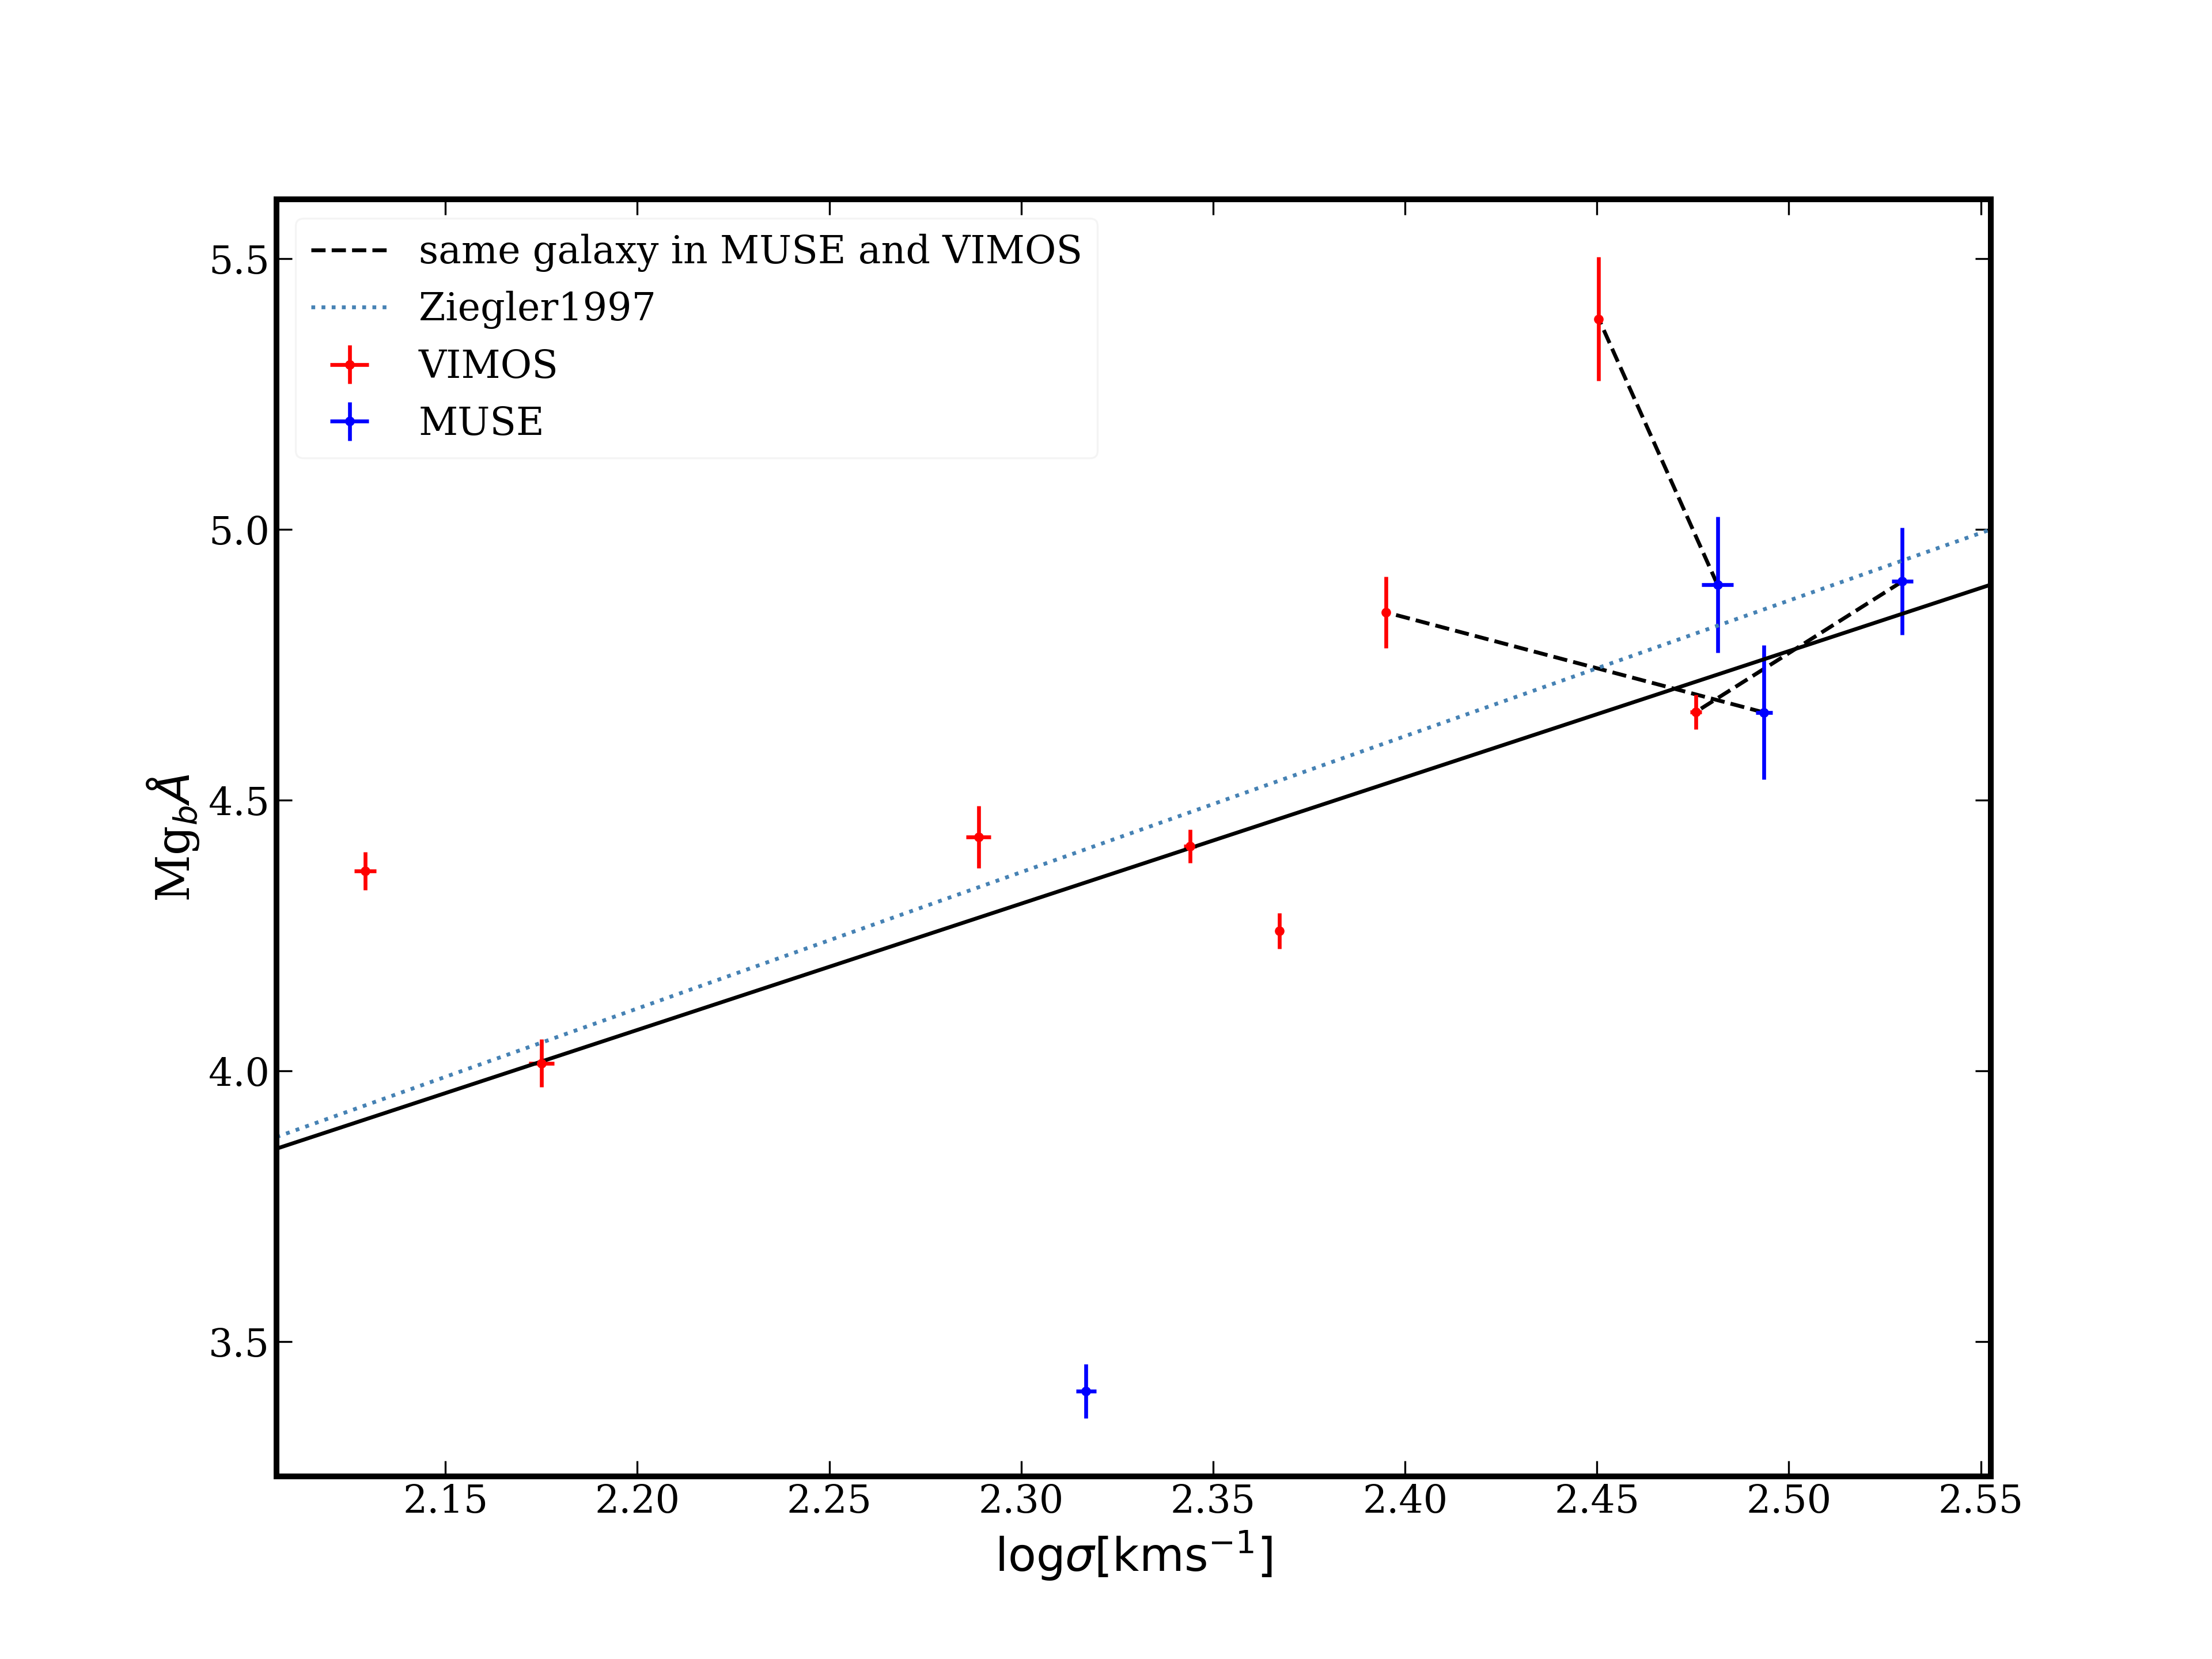
\includegraphics[width=.8\textwidth]{chapter4/Mg_sigma.png}
				\caption[Global Mg\,b--$\sigma$]{The Mg\,b -- velocity dispersion relation using a 2\arcsec aperture. We find a similar gradient to our best-fit (solid) as that found by \citet[; dotted line]{Ziegler1997}.}
				\label{fig:globalMg}
			\end{figure}

			\citet{Mehlert2003} shows the existence of the internal Mg--$\mathrm{\sigma}$ relation, but also suggests that it has a different origin to that of the global relation. They found that alpha-enhancement correlates with velocity dispersion and drives about 30\% of the global Mg--$\sigma$ relation, with metallicity variations providing the remaining 70\%. Alpha-enhancement usually has no radial gradient (while velocity dispersion is highly dependent on radius) suggesting that alpha-enhancement has no role in the internal Mg--$\sigma$ relation and it is entirely due to the metallicity radial gradient. We therefore have not shown the internal Mg -- $\sigma$ relationships. Instead we investigate radial gradients of the most-likely simple stellar populations (SSPs) in Section \ref{subsubsec:popGrad}.


		\subsubsection{Comparison to the Literature}
			\label{subsubsec:Lit}

			A comparison to the literature is difficult because of the inhomogeneous corrections applied by different authors. There are no standardized methods for accounting for emission lines from the ISM and/or stellar velocity dispersion. For example, some authors only correct for H\,$\beta$ emission, despite [\ion{O}{iii}] often being the strongest emission line in ETGs. This will effect the reliability of of Fe5015 index, since the [\ion{O}{iii}] doublet falls within its bandpasses. [\ion{N}{i}] emission will affect the Mg\,b index in the same way, although obviously not as strongly.

			Some indices are extremely sensitive to the stellar velocity dispersion correction. For example, due to the steepness of the pseudo-continuum in the G4300 index, a change of $30 \, \mathrm{km\,s^{-1}}$ in the velocity dispersion can effect the dispersion corrected index value by as much as 2\,\AA.

			When comparing to a particular paper we correct for the same effects described in the paper, but using our methods, as described in Section \ref{subsubsec:Absorption}. We use a resolution of 8.4\,\AA\ (FWHM) in order to use the transformation function provided by \citet{Vazdekis2010} to convert from Lick calibrated measurements to the Line Index System (LIS; see Section \ref{subsubsec:Absorption}). 

			Table \ref{tab:litAbsorption} summarises our comparisons to the literature. For the comparison to \citet{Vazdekis2010}, we analysed the SAURON dataset\footnote{\url{http://www.strw.leidenuniv.nl/sauron/}} \citep{Emsellem2004} using the same analysis pipeline as for our Southern Sample. 


% Should SARUON comparison be in Chapter 2 as a test of the pipeline?
			\begin{table}
				\centering
			\begin{threeparttable}
				\caption{Comparisons of measured absorption line indices to the literature.}
				\label{tab:litAbsorption}
				\begin{tabular*}{0.8\textwidth}{@{\extracolsep{\fill}}l r r r}
					\hline
					\hline
					Index 		& \multicolumn{1}{c}{N$_\mathrm{gals}$} & \multicolumn{1}{c}{Offset} & \multicolumn{1}{c}{Dispersion} \\
								& 		&\multicolumn{1}{c}{\AA}& \multicolumn{1}{c}{\AA} \\
					\hline
					\multicolumn{4}{c}{\citet{Vazdekis2010} (SAURON)} \\
					\hline
					H\,$\beta$ 	& 46		& -0.02\leavevmode\phantom{0}& 0.25\leavevmode\phantom{0}	\\
					Fe5015		& 46		& 0.66\leavevmode\phantom{0}& 0.34\leavevmode\phantom{0}	\\
					Mg\,b 		& 46		& 0.06\leavevmode\phantom{0}& 0.33\leavevmode\phantom{0}	\\
					\hline
					\multicolumn{4}{c}{\citet{Rampazzo2005} (VIMOS)} \\
					\hline
					G4300 		& 3 		& 2.29\leavevmode\phantom{0}& 0.11\leavevmode\phantom{0}	\\
					Fe4383 		& 3 		& 0.39\leavevmode\phantom{0}& 0.23\leavevmode\phantom{0}	\\
					Ca4455 		& 3 		& -0.19\leavevmode\phantom{0}& 0.09\leavevmode\phantom{0}	\\
					Fe4531 		& 3 		& 0.16\leavevmode\phantom{0}& 0.26\leavevmode\phantom{0}	\\
					H\,$\beta$ 	& 3 		& 0.17\leavevmode\phantom{0}& 0.12\leavevmode\phantom{0}	\\
					Fe5015 		& 3 		& -0.73\leavevmode\phantom{0}& 0.48\leavevmode\phantom{0}	\\
					Mg\,b 		& 3 		& -0.43\leavevmode\phantom{0}& 0.17\leavevmode\phantom{0}	\\
					\hline
					\multicolumn{4}{c}{\citet{Rampazzo2005} (MUSE)} \\
					\hline
					H\,$\beta$ 	& 2 		& -0.28\leavevmode\phantom{0}& 0.17\leavevmode\phantom{0}	\\ 
					Fe5015 		& 2 		& 0.87\leavevmode\phantom{0}& 0.34\leavevmode\phantom{0}	\\ 
					Mg\,b 		& 2 		& 0.31\leavevmode\phantom{0}& 0.14\leavevmode\phantom{0}	\\
					Fe5270 		& 2 		& -0.11\leavevmode\phantom{0}& 0.15\leavevmode\phantom{0}	\\
					Fe5335 		& 2 		& 0.08\leavevmode\phantom{0}& 0.15\leavevmode\phantom{0}	\\
					Fe5406 		& 2 		& 0.16\leavevmode\phantom{0}& 0.07\leavevmode\phantom{0}	\\
					Fe5709 		& 2 		& 0.11\leavevmode\phantom{0}& 0.10\leavevmode\phantom{0}	\\
					Fe5782 		& 2 		& -0.03\leavevmode\phantom{0}& 0.11\leavevmode\phantom{0}	\\
					NaD 		& 2 		& 0.90\leavevmode\phantom{0}& 0.41\leavevmode\phantom{0}	\\
					TiO1 (mag)	& 2 		& -0.004	& 0.003	\\
					TiO2 (mag)	& 2 		& -0.011	& 0.007	\\
					\hline
					\multicolumn{4}{c}{\citet{Ogando2008} (VIMOS)} \\
					\hline
					H\,$\beta$ 	& 6 		& 0.07\leavevmode\phantom{0}& 0.60\leavevmode\phantom{0}	\\
					Fe5015 		& 6 		& -0.09\leavevmode\phantom{0}& 0.15\leavevmode\phantom{0}	\\
					Mg\,b 		& 6 		& -0.70\leavevmode\phantom{0}& 0.08\leavevmode\phantom{0}	\\
					\hline
					\multicolumn{4}{c}{\citet{Ogando2008} (MUSE)} \\
					\hline
					H\,$\beta$ 	& 3 		& -0.04\leavevmode\phantom{0}& 0.23\leavevmode\phantom{0}	\\ 
					Fe5015 		& 3 		& -0.16\leavevmode\phantom{0}& 0.33\leavevmode\phantom{0}	\\ 
					Mg\,b 		& 3 		& -1.10\leavevmode\phantom{0}& 0.26\leavevmode\phantom{0}	\\
					Fe5270 		& 3 		& -0.66\leavevmode\phantom{0}& 0.16\leavevmode\phantom{0}	\\
					Fe5335 		& 3 		& -0.66\leavevmode\phantom{0}& 0.11\leavevmode\phantom{0}	\\
					Fe5406 		& 3 		& -0.51\leavevmode\phantom{0}& 0.06\leavevmode\phantom{0}	\\
					Fe5709 		& 3 		& -0.22\leavevmode\phantom{0}& 0.08\leavevmode\phantom{0}	\\
					NaD 		& 3 		& -1.57\leavevmode\phantom{0}& 0.16\leavevmode\phantom{0}	\\
					\hline
					\hline
				\end{tabular*}
				\begin{tablenotes}
				\footnotesize
				\note Comparisons to \citet{Rampazzo2005} are sampled at 7 radial apertures for each galaxy: 1.5, 2.5 and 10.0 arcsec and R$_e$/10, R$_e$/8, R$_e$/4 and R$_e$/2. 
				\item Col.\,1: Index. Col.\,2: Number of galaxies in comparison. Col.\,3: Offset equals the mean of the measurements from the literature subtract our measurements. Col.\,4: Dispersion equals the standard deviation of the measurements from the literature subtract our measurements.
				\end{tablenotes}
			\end{threeparttable}
			\end{table}

			We find a very large offset for the G4300 index with respect to the results of \citet{Rampazzo2005}. As noted above, this index is extremely sensitive to the stellar velocity dispersion correction and we measure an average difference in the stellar velocity dispersion to that measured by \citet{Rampazzo2005} of $21\,\mathrm{km\,s^{-1}}$. This may be enough to account for the difference in the measurements.

			We also observe that the offset in the Fe5015 index is also quite large in comparisons with \citet{Rampazzo2005} and \citet{Vazdekis2010}. In the case of the comparison with \citet{Rampazzo2005} we suggest that the difference is due to differences in method for accounting for the [\ion{O}{iii}] emission lines, however the origin of the offset is less clear in case of the comparison with \citet{Vazdekis2010}. 

			Other than G4300 and Fe5015, the comparisons show fairly consistent agreement with literature measurements although the dispersion of the comparisons are fairly large. We suggest that the translation between Lick and LIS systems may be the source of this spread.


	\subsection{Most-likely Stellar Population Models}
		\label{subsec:ssp}
		We have assumed that a given spectrum from our Southern sample can be well approximated by a SSP. We use the method described in Section \ref{subsubsec:StellarPop} to produce maps of the most-likely SSP characteristics: age ($t$), metallicity ($Z/H$) and alpha-element enhancement ($\alpha$/Fe) from the absorption line strength maps. 

		Figs.\,\ref{fig:VIMOS_pop} and \ref{fig:MUSE_pop} show the resolved most-likely stellar populations for our Southern sample. In general they show old, metal rich and alpha enhanced SSPs; qualities which ETGs are well known for. The exceptions are NGC 612 and NGC 1316. Both galaxies are described in more detail in Appendix \ref{cha:Description}, but NGC 1316 shows a very young stellar population (our fit of $t \approx 2$\,Gyr agrees with that of \citealt{Kuntschner2000}, but is conflicting with the older and less metal rich stellar population of \citealt{Koleva2011} who found $t=4.5 \pm 0.3 \,\mathrm{Gyr}$ and $\mathrm{[Fe/H]}=0.12 \pm 0.01 \,\mathrm{[Fe/H]_\odot}$ for an aperture covering the central 0.1 kpc). NGC 3557 is notable for containing a significantly younger ($t\approx 4$\,Gyr) core of about 10\arcsec\ diameter and NGC 3100 has a branch of young stars ($\approx 4$\,Gyr) along the southeast branch of the molecular gas (cyan contours).

		\begin{figure}
			\centering
			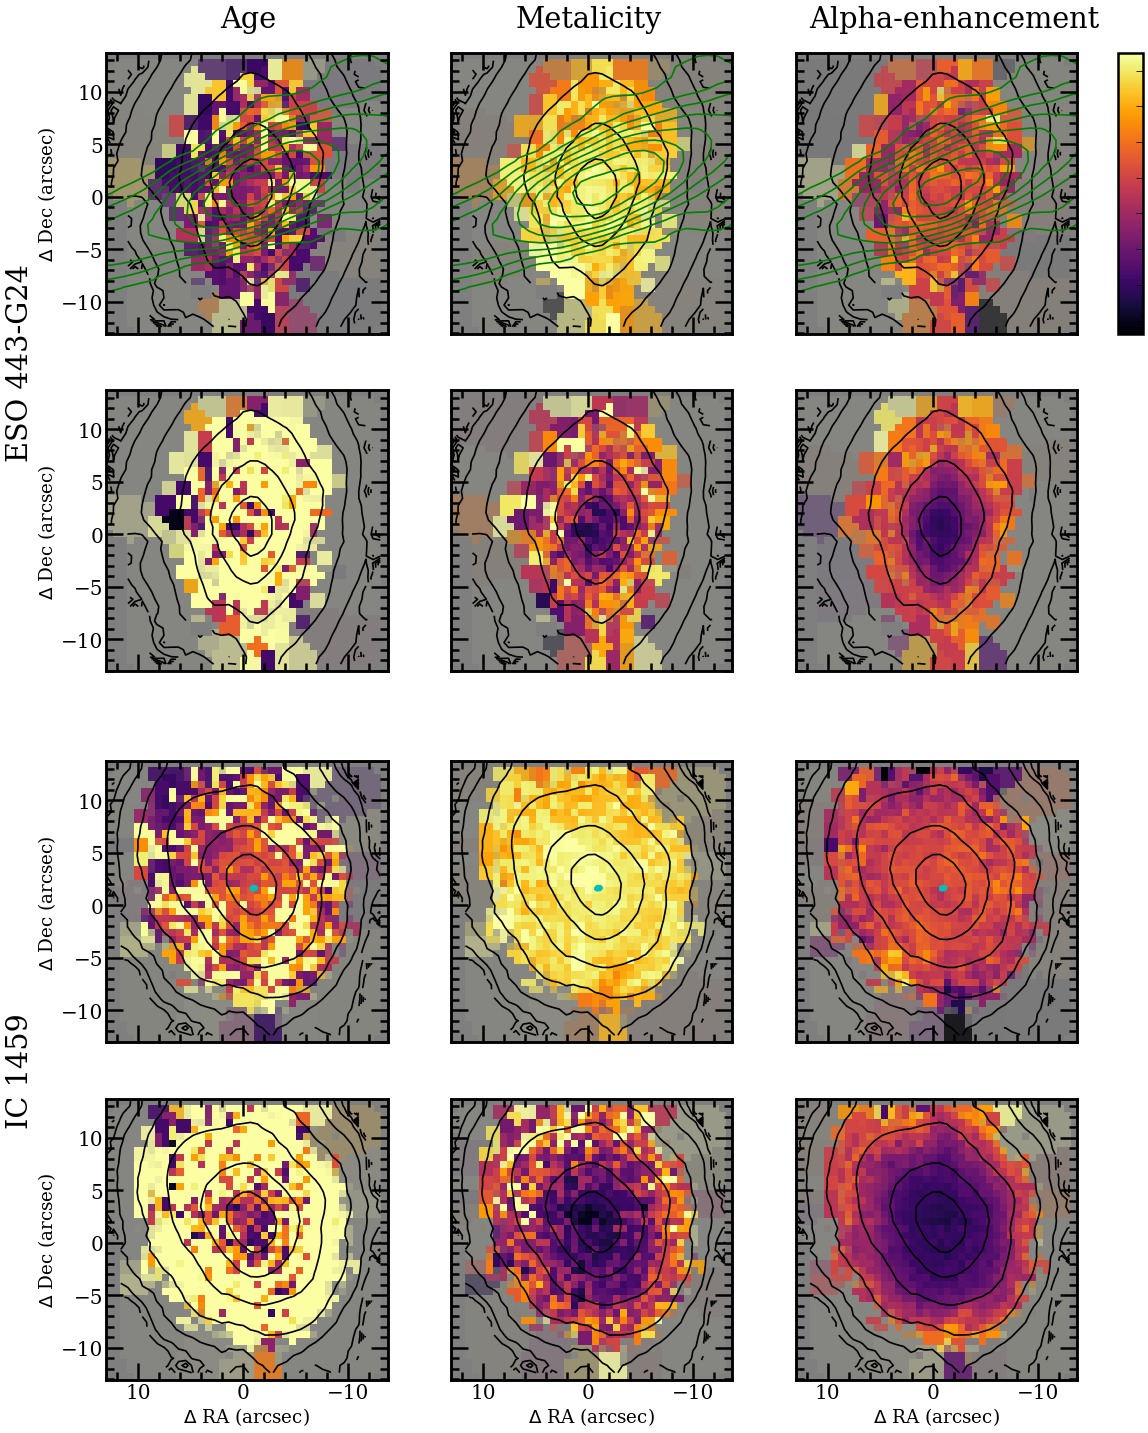
\includegraphics[height=0.63\textheight]{chapter4/vimos/pop1.png}
			\caption[VIMOS stellar population maps]{VIMOS stellar population maps: Left to right: age, metallicity and alpha enhancement; Top to bottom: ESO 443-G24 and IC 1459. Alternate rows show a given parameter its associated uncertainty. Contours are as in Fig.\,\ref{fig:VIMOS_stellar}. Limits on the colour scale are: age (and associated uncertainty) 0--15 (0--2)\,Gyr, metallicity (and associated uncertainty) -2.25--0.67 (0--0.4)\,$\mathrm{[Fe/H]_\odot}$ and alpha enhancement (and associated uncertainty) -0.3--0.5 (0-0.25)\,$\mathrm{[\alpha/Fe]_\odot}$.}
			\label{fig:VIMOS_pop}
		\end{figure}
		\begin{figure}
			\centering
			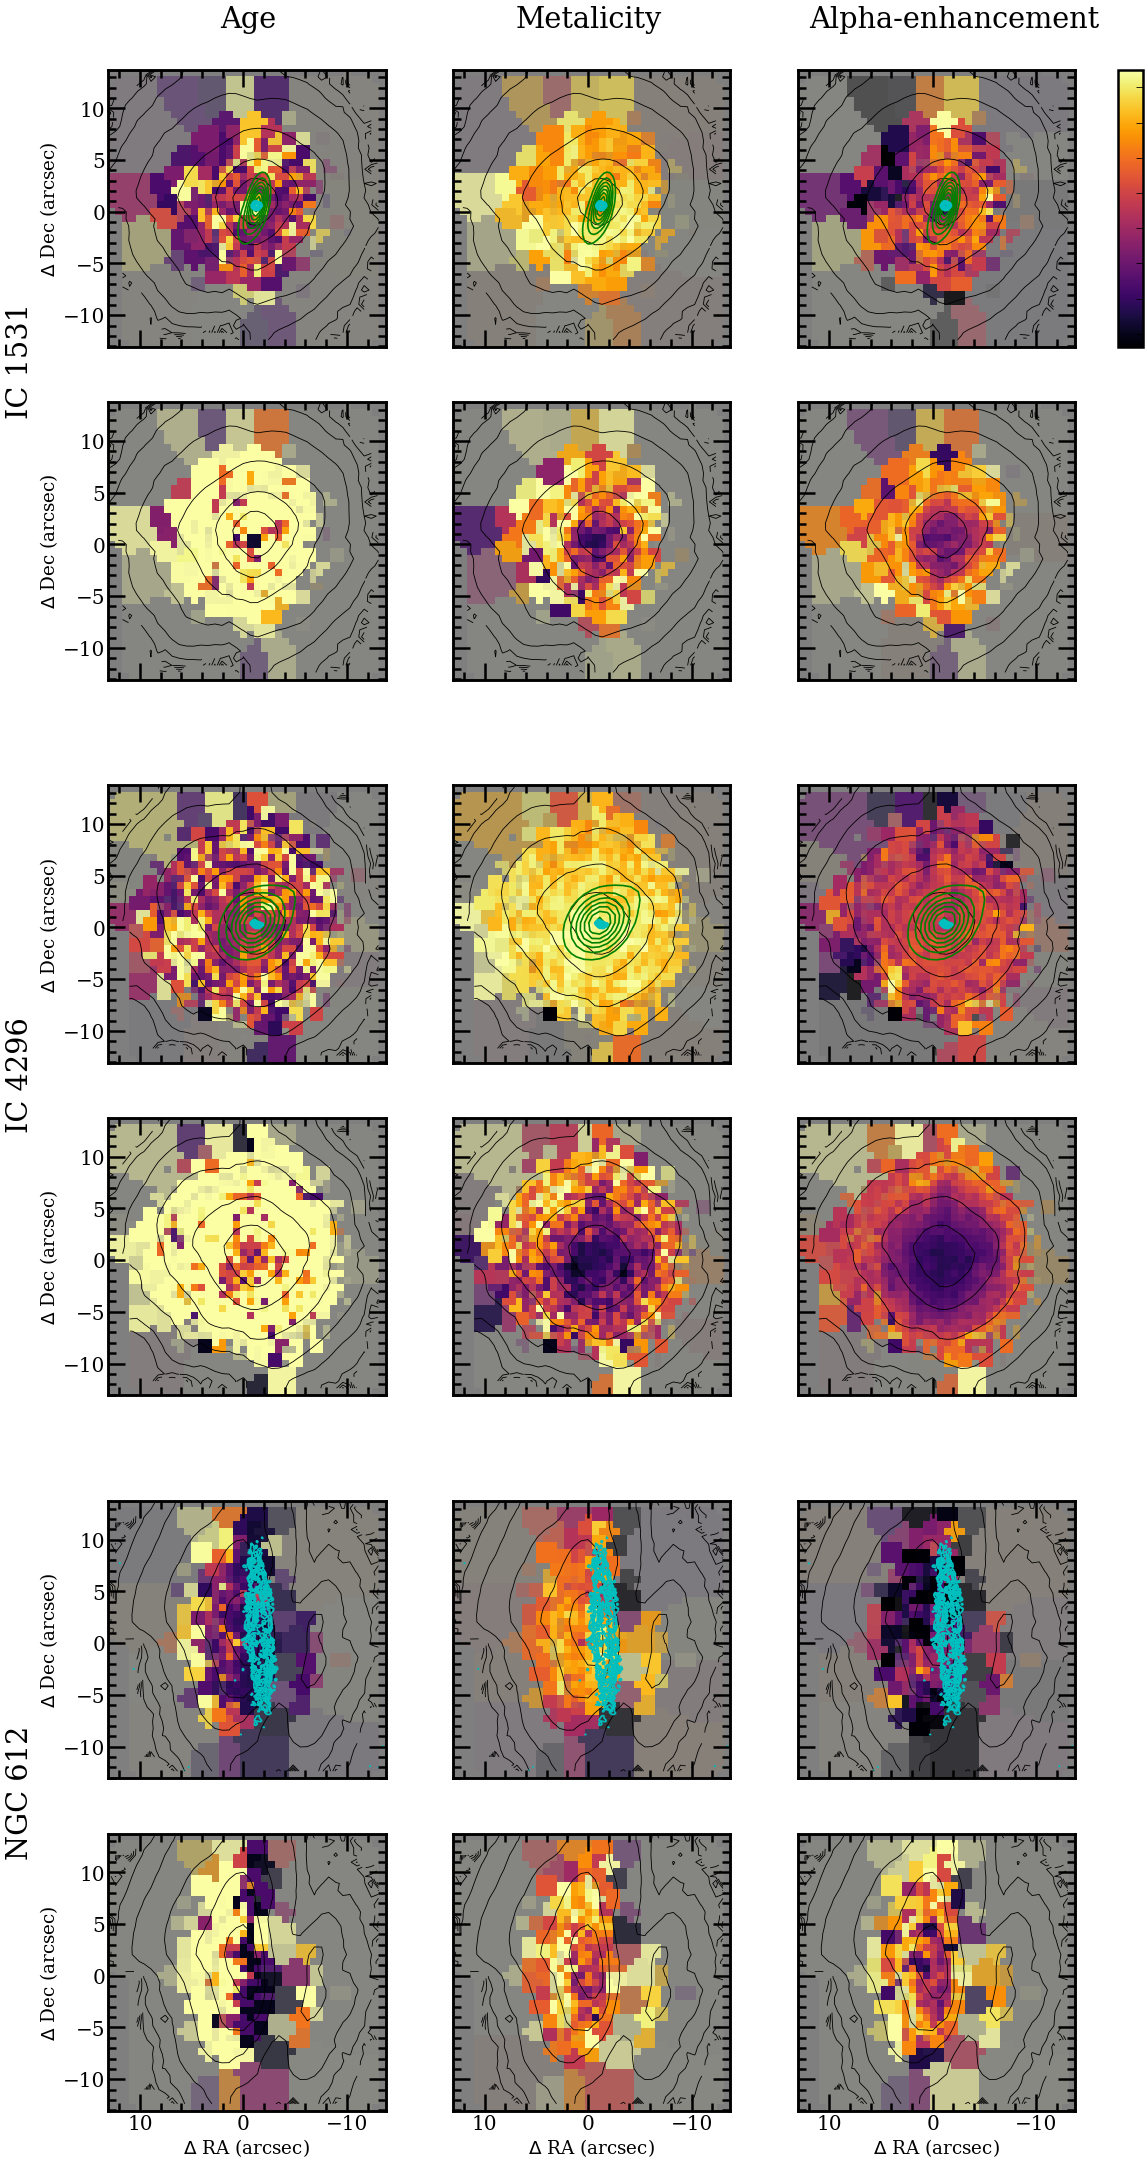
\includegraphics[height=0.94\textheight]{chapter4/vimos/pop2.png}
			\contcaption{\textit{Continued.}}% for IC 4296, NGC 612 and NGC 1399}
		\end{figure}
		\begin{figure}
			\centering
			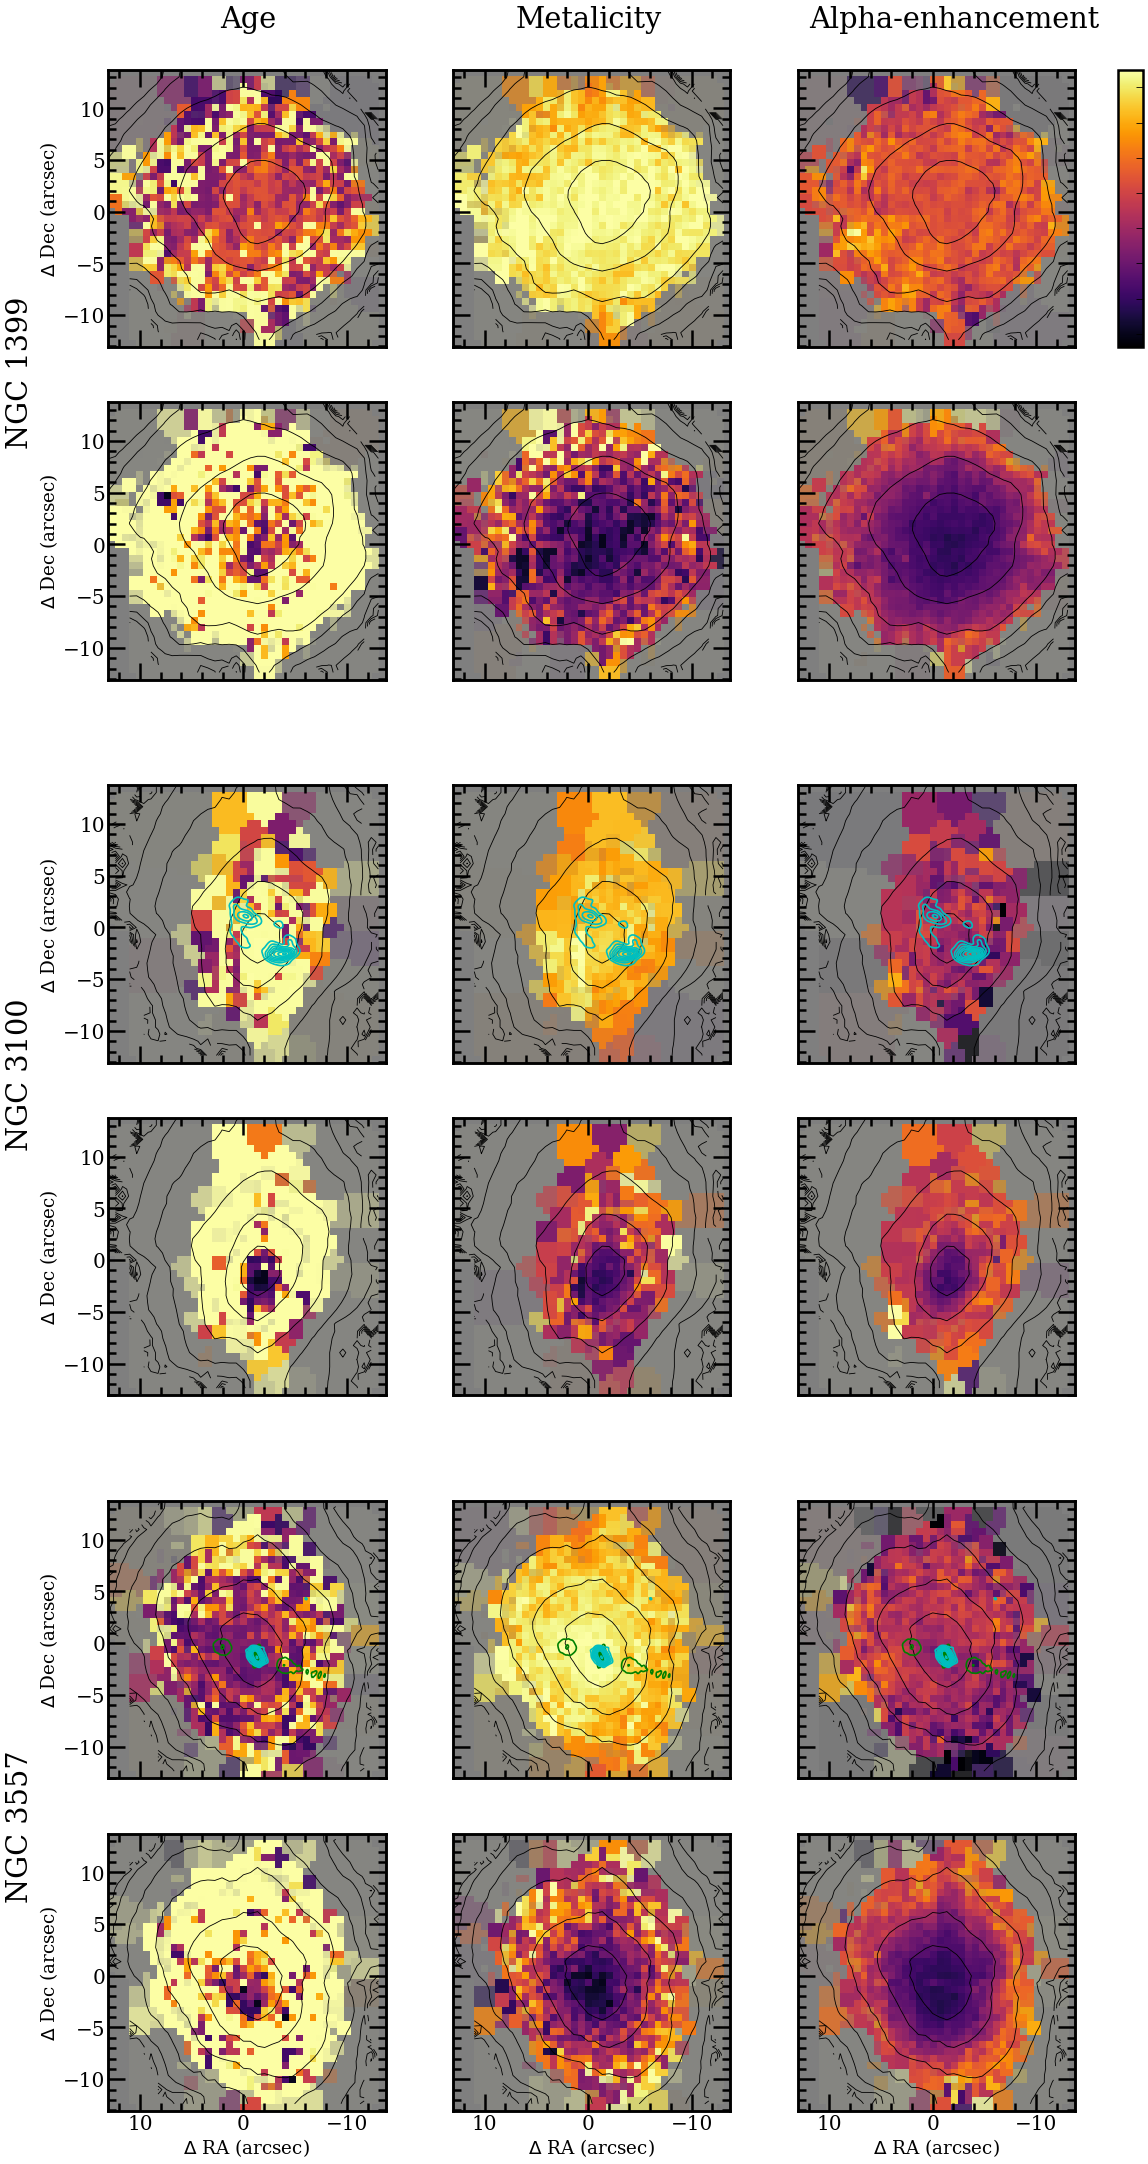
\includegraphics[height=0.94\textheight]{chapter4/vimos/pop3.png}
			\contcaption{\textit{Continued.}}% for NGC 3100, NGC 3557 and NGC 7075}
		\end{figure}
		\begin{figure}
			\centering
			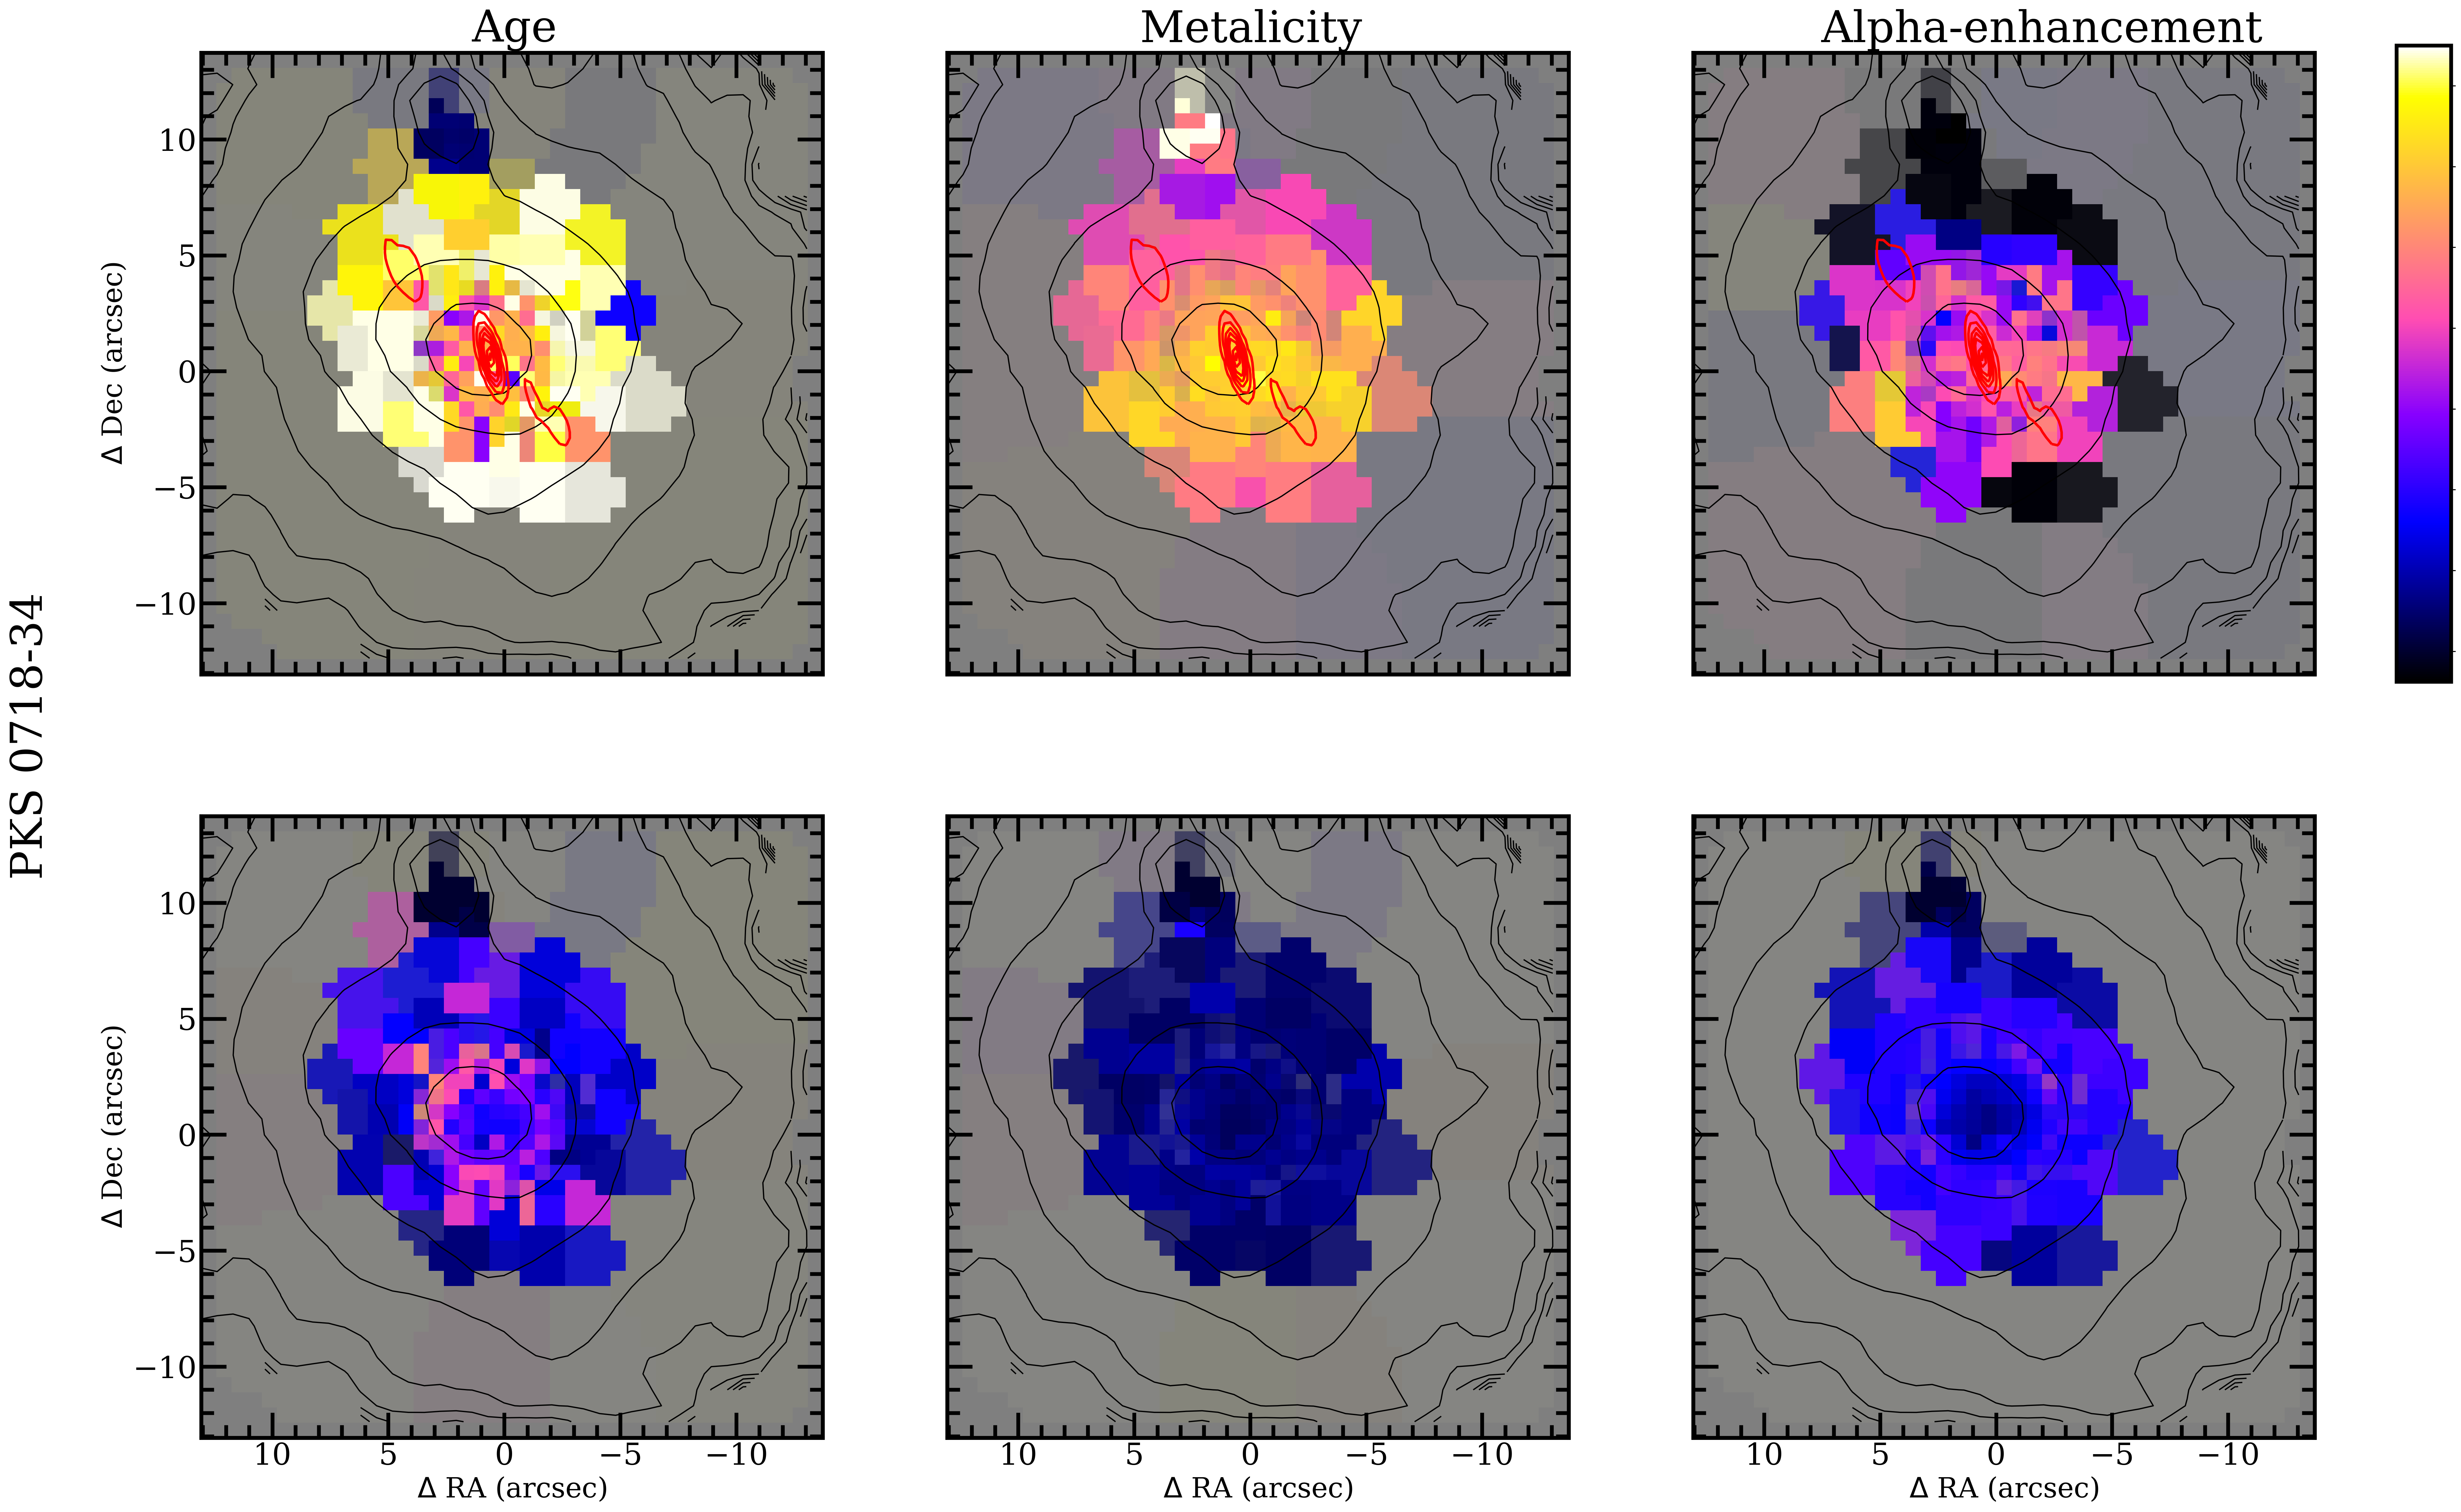
\includegraphics[height=0.63\textheight]{chapter4/vimos/pop4.png}
			\contcaption{\textit{Continued.}}% for PKS 718-34}
		\end{figure}

		\begin{figure}
			\centering
			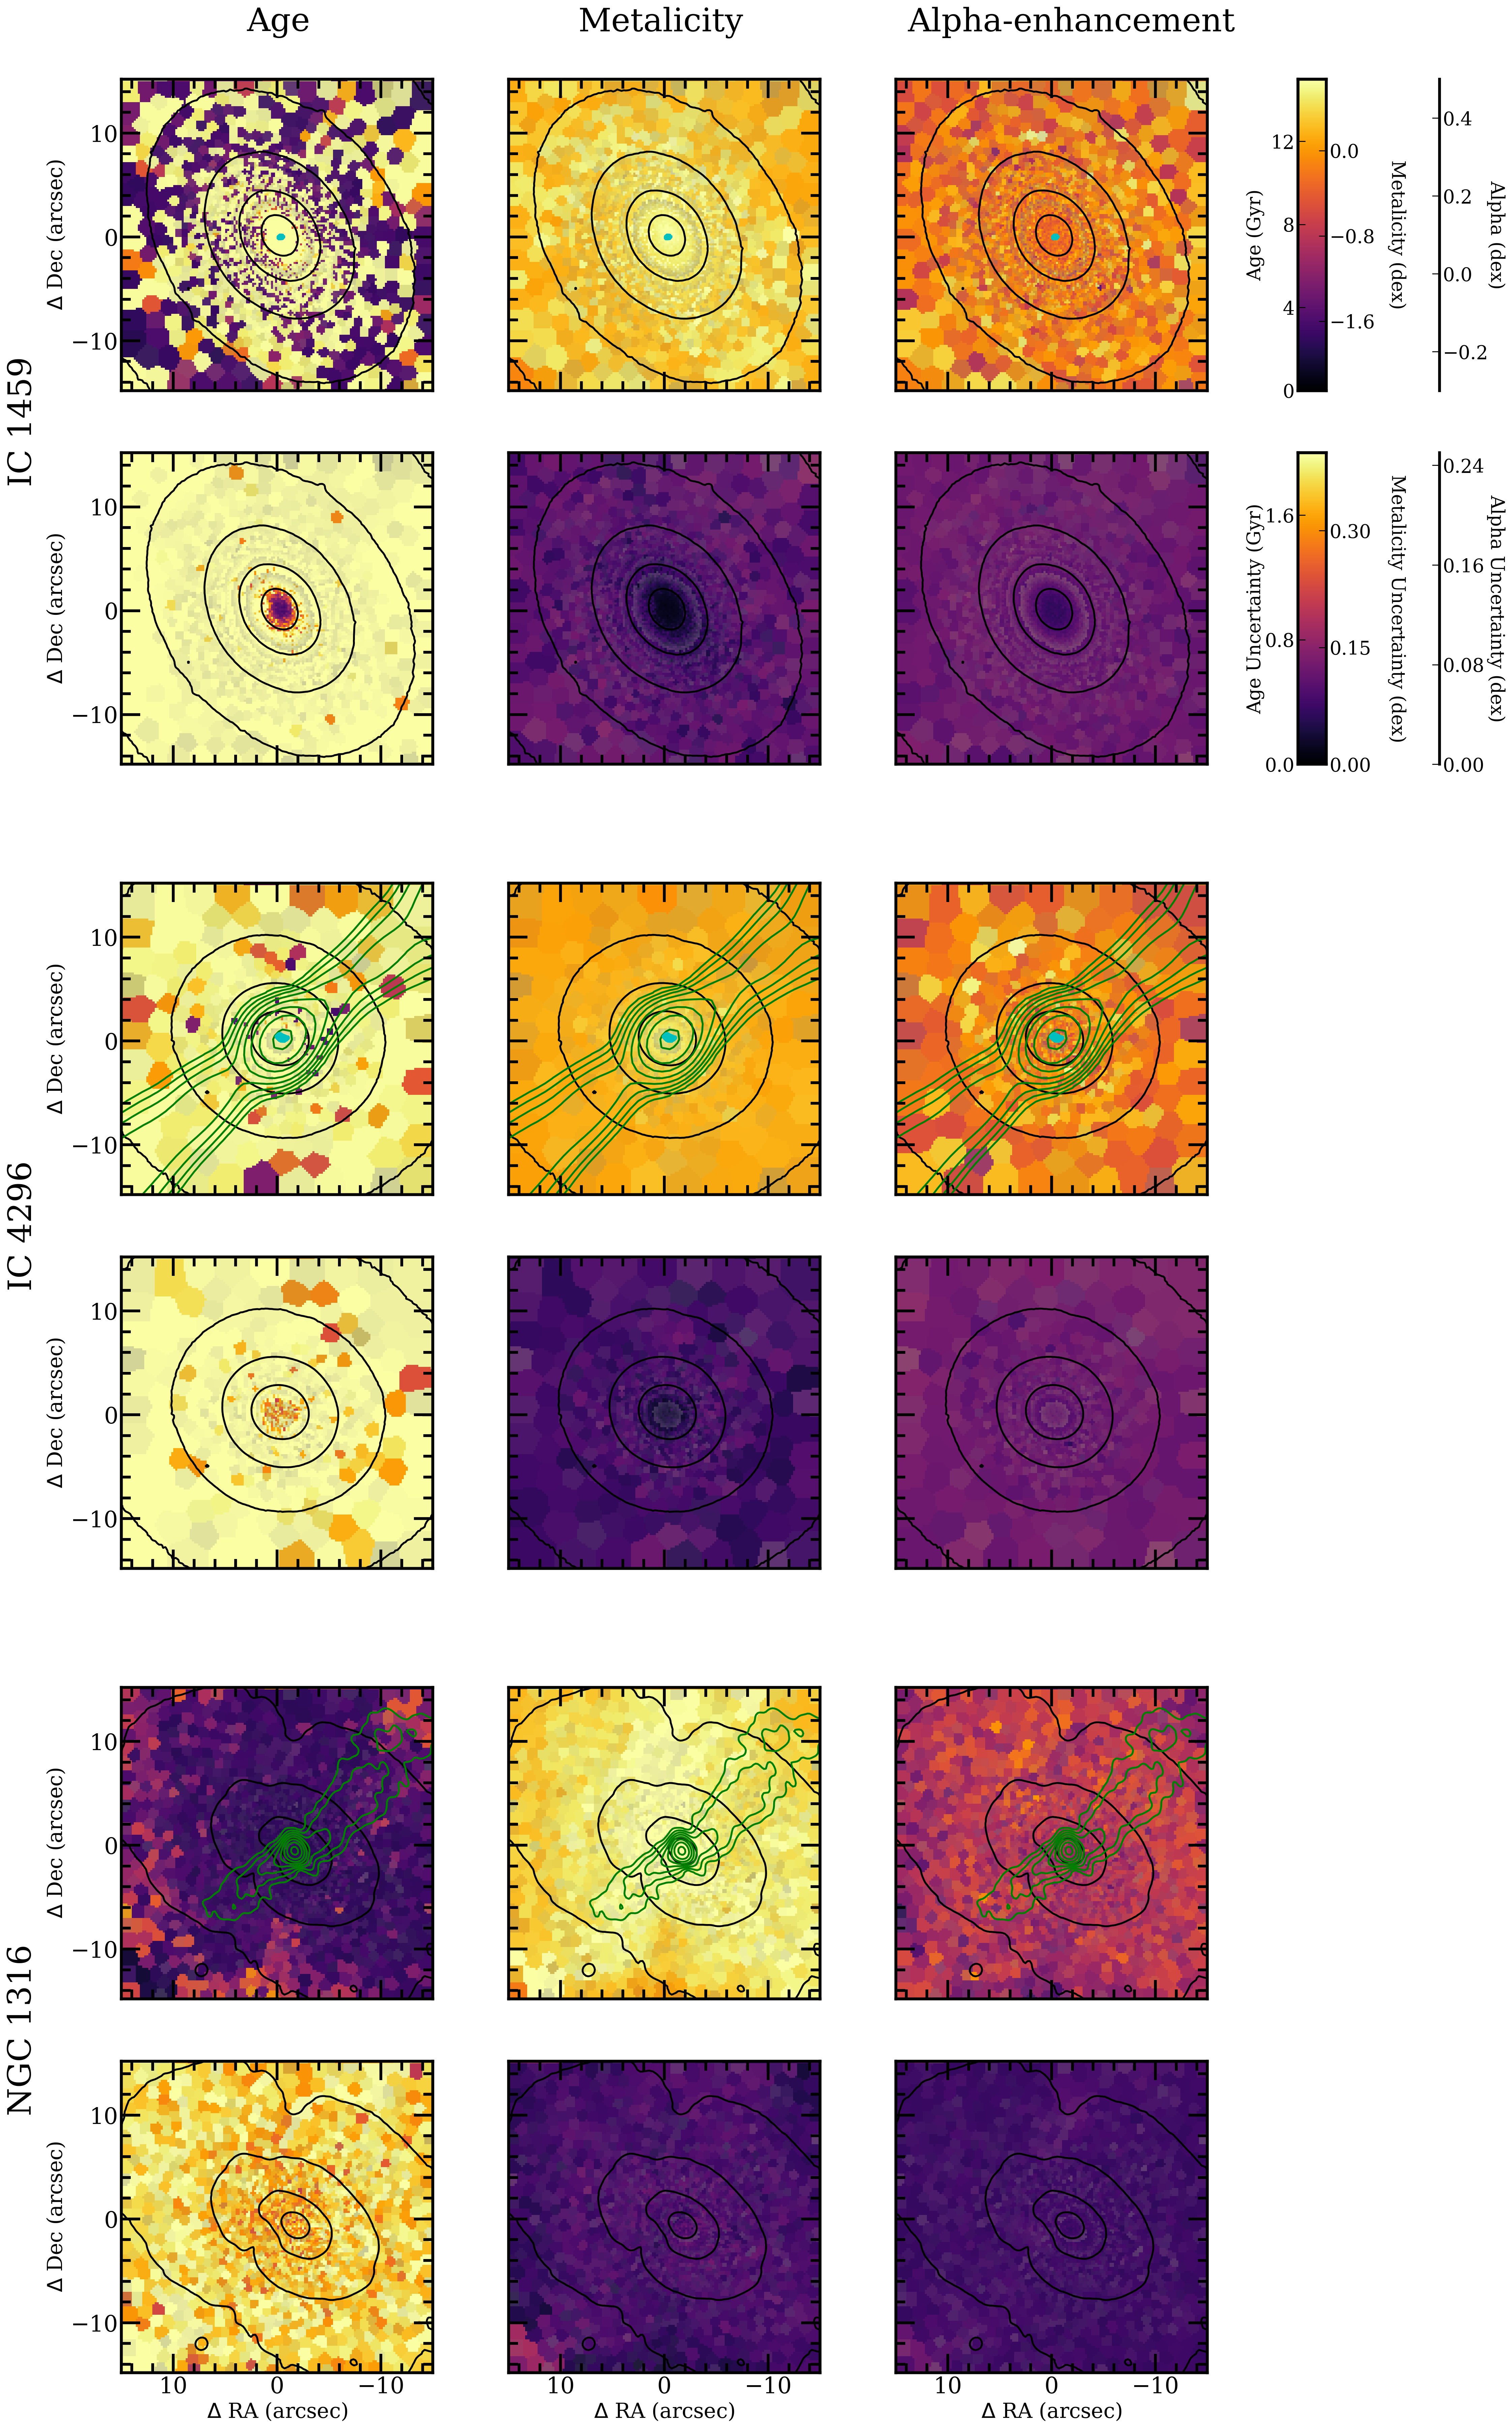
\includegraphics[height=0.94\textheight]{chapter4/muse/pop1.png}
			\caption[MUSE stellar population maps]{As in Figure \ref{fig:VIMOS_pop} but for the MUSE stellar population maps.}
			\label{fig:MUSE_pop}
		\end{figure}
		\begin{figure}
			\centering
			\includegraphics[height=0.31\textheight]{chapter4/muse/pop2.png}
			\contcaption{\textit{Continued.}}
		\end{figure}

% Could be moved to discussion?
		% If molecular (cold) gas is the fuel source that is accreted on to the the central black holes of our Southern sample in order to power the radio jets, unless it is accreted in a highly turbulent fashion, it might be expected that some of that gas might form stars \citep[e.g.][]{Collin1999, Diamond-Stanic2012, LaMassa2013}. If this is the case then a young stellar population might be expected to dominate in the very central (1--2) spaxels. We our maps show no evidence of this. 


		\subsubsection{Radial Gradients in Stellar Populations}
			\label{subsubsec:popGrad}

			\citet{Koleva2011} showed that while individual galaxies can have a wide range of radial gradients of age and metallicity, the mean gradient (within a mass bin) is uniform across a large mass range. They assume a linear relationship between $\log t$ or [Fe/H] and $\log (R/\mathrm{R_e})$. The results from our southern sample are shown in table \ref{tab:popGrad}. 

			\begin{table}
				\centering
				\caption{The radial gradients of the most-likely SSP models.}
				\label{tab:popGrad}
				\begin{tabular}{l c c}
					\hline
					\hline 
					Galaxy 	& $\Delta_\text{log age}$ & $\Delta_\text{[Fe/H]}$ \\ 
						& dex\,arcsec$^{-1}$ & [Fe/H]$_\odot$ arcsec$^{-1}$ \\
					\hline
					ESO 443-G024 & $0.019 \pm 0.013$ & $-0.01 \pm 0.02$ \\
					IC 1459 	& $0.003 \pm 0.002$ & $0.00 \pm 0.06$ \\
					IC 1531 	& $0.012 \pm 0.015$ & $0.01 \pm 0.02$ \\
					IC 4296		& $0.000 \pm 0.002$ & $0.04 \pm 0.08$ \\
					NGC 612 	& $0.068 \pm 0.060$ & $-0.11 \pm 0.02$ \\
					NGC 1316 	& $0.001 \pm 0.002$ & $0.05 \pm 0.03$ \\
					NGC 1399 	& $0.001 \pm 0.002$ & $0.10 \pm 0.09$ \\
					NGC 3100 	& $0.000 \pm 0.010$ & $-0.06 \pm 0.01$ \\
					NGC 3557 	& $0.048 \pm 0.039$ & $-0.05 \pm 0.05$ \\
					NGC 7075 	& $0.007 \pm 0.011$ & $-0.07 \pm 0.02$ \\
					PKS 718-34  & $0.002 \pm 0.009$ & $-0.17 \pm 0.03$ \\
					\hline
					\hline
				\end{tabular}
			\end{table}

			We find average gradients of $\Delta_\text{log age} = 0.014\pm0.007 \,\mathrm{dex \, arcsec^{-1}}$ and $\Delta_\text{[Fe/H]} = -0.03\pm0.01 \, \mathrm{[Fe/H]_\odot \, arcsec^{-1}}$. This is consistent with \citet{Koleva2011} who, for elliptical galaxies found average gradients of $0.06\pm0.09 \, \mathrm{dex \, arcsec^{-1}}$ and $-0.26\pm0.08 \, \mathrm{[Fe/H]_\odot \, arcsec^{-1}}$ for the age and metallicity gradients, respectively. For S0s they find flatter corresponding gradients of $0.01\pm0.11\, \mathrm{dex \, arcsec^{-1}}$ and $-0.12\pm0.13\, \mathrm{[Fe/H]_\odot \, arcsec^{-1}}$. 

% SSP -- sigma relation here?



	\subsection{Kinematically-Decoupled Cores}
		\label{subsec:popKDC}

		\citet{Kuntschner2010} found that kinematically-decoupled cores (KDCs) exist in two classes: they are either small or contain an old stellar population. The size of the KDC is defined as the radius of the region surrounding the KDC where the superposition of the two components (the KDC and the host galaxy) results in a local minimum in the mean velocity. The age of the most-likely SSP model for the spatially integrated spectrum within an aperture 1\arcsec\ on the centre of the galaxy is taken as the KDC's age.

		The small KDCs tend to be found in fast rotators with galaxy-wide young stellar populations and still younger stellar populations within the KDC. They also tend to be counter-rotating or very close to counter-rotating with respect to the host galaxy (it is too difficult to distinguish the the co-rotating KDCs that should be expected from their host galaxies). \citet{Kuntschner2010} suggests that the dominance of the stellar light of these KDCs over the other stars in the centre of the galaxies will reduce as time passes. As such, it is thought that old, small KDCs do exist, but they are not observable. \citet{Kuntschner2010} further propose that these KDCs are the result of gas accreted into the galaxy, settling into a counter-rotating disc near the centre of the galaxy, before forming the stars that make up the KDC. 

		The large KDCs are typically embedded in slow rotators. They have no limit on the age of their stellar populations suggesting that the stars within the KDC dominate in total mass as well as surface brightness. Thus, they do not fade into their host galaxies as they age unlike the small KDCs. \citet{Bois2011} showed major mergers may well result in such large KDCs if the initial spin axis of the progenitor galaxy with the lowest bulge-to-disk ratio (later-type) is anti-parallel to the orbital angular momentum vector. 

		In Fig.\,\ref{fig:KDC} we show the age and size of the 3 KDCs hosted by galaxies in our Southern sample. We include PKS 718-34 here but stress it is only tentatively classified as containing a KDC. As can be seen from Fig.\,\ref{fig:KDC}, PKS 718-34 would be an extremely large KDC, but is still is consistent with the findings of \citet{Kuntschner2010}.

		\begin{figure}
			\centering
			\includegraphics[width=.7\textwidth]{chapter4/KDC_size_age.png}
			\caption[KDC dichotomy]{The KDC size -- age relation. KDCs exist in two classes: old or small. VIMOS is in red, MUSE in blue and SAURON from \citet{Kuntschner2010} in black and gray for fast and slow rotators respectively.}
			\label{fig:KDC}
		\end{figure}
	
\section{Discussion}
	\label{sec:stellarDiscussion}
	In this chapter we have shown that in terms of the stellar kinematic properties and stellar populations, our radio-selected Southern sample are no different to ordinary optically-selected ETGs. 
	Our sample shows a mixture of of regularly- and non-regularly-rotating behaviours, with both classes showing evidence of consistency with observations of the intrinsic shapes of ordinary regular and non-regular rotators. 
	We also classify our sample galaxies into fast- and slow-rotators and find a consistent fraction of slow-rotators to the ordinary ETG samples of the A+M sample, once the difference in the mass distribution between our Southern sample and the A+M sample are taken into account. 

	
% better word than common?

	% We interpret S0 galaxies as well inclined discs, but we should should however make explicit the distinction between fast rotators and disc galaxies. We define disc galaxies as rotationally supported with $\frac{|v_\text{int}|}{\sigma} > 1$, where $v_\text{int}$ is the peak intrinsic velocity. It is not uncommon to have dispersion-dominated fast-rotators. Assuming our fast rotators to be axisymmetric (i.e. the intrinsic ellipticity is 1 such that $\frac{|v_\text{int}|}{\sigma} = \frac{|v|}{\sigma \cos\sin^{-1}\epsilon}$), we find only NGC 612 to be a true disc with $\frac{|v_\text{int}|}{\sigma} = 1.04$, consistent with is classification as one of the few radio-loud S0s \citep{}. NGC 3100 and NGC 3557 are the next closest, both with $\frac{|v_\text{int}|}{\sigma} \approx 0.8$. 

	% This suggests that while the formation of jet-mode AGN does not explicitly require the galaxy disc to have been destroyed (presumably via a dry major merger), such an event significantly enhances the likelihood of it occurring.

	In terms of stellar populations, we find a remarkably similar gradient to the central Mg\,b verse stellar velocity dispersion relation to that of \citet{Ziegler1997}. Most of the galaxies in our Southern sample show typical ETG behavior: old, metal rich stellar populations, with a few exceptions: NGC 612 and NGC 1316 are both significantly younger than most ETGs and NGC 3557 has a young core. All are described in more detail in Appendix \ref{cha:Description} 
% Does NGC 3557 have a large -ve age gradient?  

	Radio-loud lenticular (S0) galaxies are extremely rare with only a handful of known cases \citep[e.g.][]{Heckman1982, Morganti2011}, presumably due to the associated mass functions of both S0s and radio galaxies: both massive S0s and non-massive radio galaxies are rare, with a similar transition masses from rare to more numerous. NGC 612 is one of those rare cases. 	

	Finally, if molecular (cold) gas is the fuel source that is accreted on to the the central black holes of our Southern sample in order to power the radio jets, unless it is accreted in a highly turbulent fashion, it might be expected that some of that gas might form stars \citep[e.g.][]{Collin1999, Diamond-Stanic2012, LaMassa2013}. If this is the case then a young stellar population might be expected to dominate in the very central (1--2) spaxels. We our maps show no evidence of this. 
\chapter{Ionized Gas Distribution, Kinematics and Ionization}
	\label{cha:gas}
The interstellar medium (ISM) of early-type galaxies (ETGs) has several components: a diffuse hot ($\sim 10^7 \, \mathrm{K}$) X-ray halo (with typical mass $10^8$--$10^{10} \, \mathrm{M_\odot}$); a warm ($\sim 10^4 \, \mathrm{K}$) ionized gas component ($10^2$--$10^5 \, \mathrm{M_\odot}$), which can be more clumpy; and cold ($<10^2 \, \mathrm{K}$) atomic and molecular gas ($10^6$--$10^8 \, \mathrm{M_\odot}$), which is generally confined to small (kpc or less) clouds. In this chapter we study the spatially-resolved properties of the ionized gas component of radio galaxies (RGs), exploiting the emission lines in the VIMOS and MUSE datacubes of the Southern Sample.

Using the methods described in Section \ref{subsec:EmissionFit}, we find the best-fit line-of-sight velocity distribution (LOSVD; assumed to be Gaussian and parametrised by the mean velocity and velocity dispersion only) of the emission lines in each bin. As described in \ref{subsec:EmissionFit}, all emission lines are fit with the same LOSVD, but each with its own flux. In the cases of the [\ion{O}{iii}], [\ion{O}{i}] and [\ion{N}{ii}] doublets, the two components of the doublets are fit with a fixed flux ratio of 1:0.34. The [\ion{N}{i}] doublet has a fixed ratio of 1:0.65 \citep{Safier1992}. The two components of the [\ion{O}{ii}] and [\ion{S}{ii}] doublets are fit independently.

This chapter is structured as follows. Firstly in Section \ref{sec:gasFlux} the flux and equivalent-width maps of each emission line in the respective wavelength range of VIMOS and MUSE are shown. Gas masses are calculated and upper limits estimated in the cases of non-detections (see Section \ref{sec:GasFlux}). Secondly, in Section \ref{sec:GasKin} the kinematics of the ionized gas is discussed. Thirdly, the likely sources of the gas ionization are investigated, making use of several emission line diagnostics (Section \ref{sec:Diagnostics}). The results for each galaxy in the Southern Sample are summarised in Table \ref{tab:gasMass}. Finally, we conclude in Section \ref{sec:gasDiscussion} with a discussion of the results of this chapter.


\begin{table}
	\centering
\begin{threeparttable}
	\caption{Gas masses of the Southern Sample galaxies.}
	\label{tab:gasMass}
	% \begin{tabular*}{\textwidth}{@{\extracolsep{\fill}}l r r r l}
	\begin{tabular}{l c c c c}
		\hline
		\hline
		Galaxy & \multicolumn{2}{c}{\ion{H}{ii} Mass} & Balmer & LINER/ \\
		& VIMOS\tnote{a} & MUSE & Decrement & Seyfert \\
		& ($\log\mathrm{M_\odot}$) & ($\log\mathrm{M_\odot}$) & \\
		\hline
		ESO 443-G024 & $5.31 \pm 0.01$ 	& --  		& -- & No detections \\
		IC 1459 	& $5.25 \pm 0.01$	& $5.51 \pm 0.01$ & $4.57 \pm 0.06$ & LINER-AGN\\
		IC 1531 	& $5.04 \pm 0.01$	& -- 		& -- & Seyfert 2\\
		IC 4296		& $5.43 \pm 0.01$	& $< 4.14$ 	& $<10.9$\tnote{b} & LINER-AGN \\
		NGC 612 	& $6.21 \pm 0.01$ 	& -- 		& -- & LINER-AGN \\
		NGC 1316 	& -- 				& $ 5.29 \pm 0.01$ & $3.54 \pm 0.05$ & LINER-AGN \\
		NGC 1399 	& $3.94 \pm 0.02$ 	& $ 4.54 \pm 0.01$ & \tnote{c} & LINER \\
		NGC 3100 	& $5.27 \pm 0.01$	& -- 		& -- & Seyfert 2 \\
		NGC 3557 	& $4.89 \pm 0.01$ 	& -- 		& -- & LINER/Retired \\
		NGC 7075 	& $5.36 \pm 0.01$	& -- 		& -- & LINER \\
		PKS 718-34  & $< 5.08$	 		& -- 		& -- & No detections \\
		\hline
		\hline
	\end{tabular}
	\begin{tablenotes}
	\footnotesize
	\note Col.\,1: Galaxy. Col.\,2: \ion{H}{ii} mass derived from the H$\beta$ line in the VIMOS data, assuming a Balmer decrement of 2.85. Col.\,3: \ion{H}{ii} mass derived from the H$\alpha$ line in the MUSE data. Col.\,4: Balmer decrement measured from the MUSE data. Col.\,5: Main source of ionizing radiation (see Section \ref{sec:Diagnostics} for a description of the different classes). A -- means we have no data.
	\item [a] The VIMOS flux calibration and thus the derived gas masses are only approximate (see Section \ref{subsec:VIMOSreduction} for more detail on the flux calibration).
	\item [b] H$\beta$ was not detected with A/N $> 2.5$, so the fit is unreliable (hence an upper limit). 
	\item [c] H$\beta$ was not detected, so the formal measured Balmer decrement is infinite. 
	\end{tablenotes}
\end{threeparttable}
\end{table}


\section{Ionized Gas Distribution}
	\label{sec:GasFlux}

	\subsection{Maps}
		\label{subsec:GasMaps}
		Images of the Southern Sample galaxies in the [\ion{O}{iii}]$\lambda\lambda$4957,5007 lines are shown in Figs.\ \ref{fig:VIMOS_OIII} and \ref{fig:MUSE_OIII}. Only 4 galaxies of the Southern Sample have emission lines detected outside of their central region (IC 1459, NGC 612, NGC 1316 and NGC 3100; see Figs.\,\ref{fig:VIMOS_OIII} and \ref{fig:MUSE_OIII}). Of the remaining 7 galaxies, NGC 1399 and PKS 718-34 have no detection of H$\beta$ in their spatially-resolved map (although we do detect H$\beta$ in the spatially-integrated spectrum of NGC 1399; see Section \ref{subsec:GasMass}), while the other 5 galaxies are only detected in their centre. All other emission lines have similar distributions, but with different fluxes.%, with the exception of NGC 612, where the significant cloud in [\ion{O}{iii}] to the south of the centre of the galaxy is not seen in H$\beta$ (see Fig.\,\ref{fig:NGC612_Hb}). 


		\begin{figure}
			\centering
			\includegraphics[width=\textwidth]{chapter5/vimos/Hb.png}
			\caption[VIMOS \bracket{\ion{O}{iii}} maps]{VIMOS [\ion{O}{iii}]$\lambda\lambda$4957,5007 maps. Total flux contours (isophotes) are shown in black, \ce{^{12}CO(2-1)} contours from ALMA in cyan, and radio continuum contours from VLA in green. The radio band shown depends on the spatial resolution and extent of the datasets available, selected to best match our IFS data.\label{fig:VIMOS_OIII}} 
			
		% \end{figure}
		% \begin{figure}
		% 	\centering
			\vspace{\floatsep}
			\includegraphics[width=\textwidth]{chapter5/muse/Hb.png}
			\caption[MUSE \bracket{\ion{O}{iii}} maps]{MUSE [\ion{O}{iii}]$\lambda\lambda$4957,5007 maps.\label{fig:MUSE_OIII}} 
			
		\end{figure}


		

		% \begin{figure}
		% 	\centering
		% 	\includegraphics[width=0.4\textwidth]{chapter5/vimos/ngc0612_Hb.png}
		% 	\caption[NGC 612 H$\beta$ image]{NGC 612 H$\beta$ map showing a large cloud to the south of the centre of the galaxy, which is not present in the H$\beta$ map (see Fig.\ref{fig:VIMOS_Hb}).} 
		% 	\label{fig:NGC612_Hb}
		% \end{figure}


		% Because equivalent width is not dependent on overall flux (except for the initial detection threshold: a line must be detected in order to observe its equivalent width), it can be used to highlight local structures that cannot be seen in flux maps. The equivalent width maps for each emission line for each galaxy in the Southern Sample are shown in Figs.\,\ref{fig:VIMOS_ew} and \ref{fig:MUSE_ew}. 

		% \begin{figure}
		% 	\centering
		% 	\includegraphics[width=\textwidth]{chapter5/vimos/ew.png}
		% 	\caption[VIMOS equivalent width maps]{VIMOS equivalent width maps.} 
		% 	\label{fig:VIMOS_ew}
		% \end{figure}
		% \begin{figure}
		% 	\centering
		% 	\includegraphics[width=\textwidth]{chapter5/muse/ew.png}
		% 	\caption[MUSE equivalent width maps]{MUSE equivalent width maps.} 
		% 	\label{fig:MUSE_ew}
		% \end{figure}

	\subsection{Gas Masses}
		\label{subsec:GasMass}

		Total ionized gas masses are derived using the prescription of \citet{Sarzi2005}. This is a very rough calculation and the values should not be used for quantitative applications. The approach follows \citet{Kim1989}, whereby
		\begin{equation}
			\left(\frac{M_\text{\ion{H}{ii}}}{M_\odot}\right) = 280 \left(\frac{D}{10\, \mathrm{Mpc}}\right)^2 \left(\frac{F(\mathrm{H\alpha})}{10^{-14} \, \mathrm{erg \, s^{-1} \, cm^{-2}}}\right) \left(\frac{10^3 \, \mathrm{cm^{-3}}}{n_\mathrm{e}}\right) \, ,
		\end{equation}
		where $M_\text{\ion{H}{ii}}$ is the total mass of \ion{H}{ii} in the galaxy, $D$ is the galaxy distance, and $F(\mathrm{H\alpha})$ is the total observed galaxy H$\alpha$ flux. This method assumes an electron density $n_\mathrm{e} = 100 \, \mathrm{cm^{-3}}$, a temperature of $10^4$ K and case-B recombination (electrons above 13.6\,eV are not reabsorbed; e.g.\ \citealt[p.\,74]{Osterbrock1974}). Like \citet{Sarzi2005}, we only claim a detection if the amplitude-to-noise ratio (A/N) is $>4$ for [\ion{O}{iii}] and $>2.5$ for H$\beta$ or H$\alpha$. Since most of the gas is centrally concentrated, a large field of view, often only serves to increase the noise (thus reducing A/N). 
		% Our lower limits on the gas mass, are set by the mass measured from the largest aperture that still meets our detection criteria. This would be the gas mass of the galaxy if there was no gas at larger radii. 
		Upper limits are calculated using the $1\sigma$ noise level (see Section \ref{subsec:EmissionFit}) or the H$\alpha$ (H$\beta$, in the case of VIMOS data) flux measurement that does not meet out A/N criterion, whichever is larger, assuming that the gas is distributed over the entire field of view.


		
		

% So what?




\section{Ionized Gas Kinematics}
	\label{sec:GasKin}
	In Figs.\,\ref{fig:VIMOS_Gaskine} and \ref{fig:MUSE_Gaskine}, we show maps of the mean velocity and velocity dispersion of the ionized gas for the 4 galaxies with extended emission lines, IC 1459, NGC 612, NGC 1316 and NGC 3100. Due to that fact that, unlike stars, gas is dissipational, it is to be expected th at given sufficient time, the ISM will always settle into a disc. These maps show that the ISM of the Southern sample galaxies varies from largely settled discs in IC 1459 and NGC 612 to more disordered kinematics of NGC 3100 and a possible inflow in NGC 1316.

	\begin{figure}
		\centering
		\includegraphics[height=0.47\textheight]{chapter5/vimos/kin.png}
		\caption[VIMOS ISM kinematic maps]{VIMOS ISM kinematic maps. Left to right: mean velocity and velocity dispersion maps. Alternate columns show a given parameter and its associated uncertainty. Top to bottom: IC 1459, NGC 612 and NGC 3100. Contours are as in Fig.\ \ref{fig:VIMOS_OIII}. Colour scale ranges are: mean velocity maps -360 to 360\,$\mathrm{km \, s^{-1}}$ (except for NGC 3100 which has a range of -100 to 100\,$\mathrm{km \, s^{-1}}$), mean velocity uncertainty 1 to 15\,$\mathrm{km \, s^{-1}}$, velocity dispersion 35 to 200\,$\mathrm{km \, s^{-1}}$, and velocity dispersion uncertainty 1 to 20\,$\mathrm{km \, s^{-1}}$.} 
		\label{fig:VIMOS_Gaskine}
	\end{figure}

	\begin{figure}
		\centering
		\includegraphics[height=0.31\textheight]{chapter5/muse/kin.png}
		\caption[MUSE ISM kinematic maps]{As Fig.\ \ref{fig:VIMOS_Gaskine} but for the MUSE ISM kinematics.}
		\label{fig:MUSE_Gaskine}
	\end{figure}


% Separate section?
	% \subsection{Misalignment of Gas}
	% 	\label{subsec:Gasmisaligment}
	It is immediately clear when comparing the mean stellar velocity maps (Figs.\,\ref{fig:VIMOS_stellar} and \ref{fig:MUSE_stellar}) to the mean gas velocity maps (Figs.\,\ref{fig:VIMOS_Gaskine} and \ref{fig:MUSE_Gaskine}) that where gas is detected, its angular momentum is not often aligned with that of the stars. A misalignment between the kinematics of the stars and gas suggests an external origin for the gas (e.g.\ accretion or wet merger). However it should be noted that the conversus is not necessarily true: aligned kinematics is consistent with an internal origin (e.g.\ stellar-mass loss), but it does \emph{not} require it \citep[e.g.][]{Davis2011a}. 

	We now comment on each galaxy in turn.

	\paragraph{IC 1459} has ionized gas counter-rotating with respect to the stellar kinematically-decoupled core, and also rotating independently from the rest of the galaxy. The gas is rotating with a mean velocity an order of magnitude higher than that of the stars (outside of the KDC). As the stellar disc did not survive the merger even that created the KDC, it is unlikely that the gas in IC 1459 progenitor galaxy survived. The lost gas may, however, have been re-accreted. Alternatively, the ISM may have yet another external origin. 

	\paragraph{NGC 612} has well aligned stellar and gaseous kinematics. The misalignment between the position angle of the stellar and gas kinematics (using the method described in Section \ref{subsec:Misalignment}) is just $1\fdg0\pm0\fdg7$, consistent with an internal origin for the gas. This adds to the evidence (see Section \ref{sec:NGC612}) that NGC 612 has not undergone a major merger (major mergers exhaust galaxies of their gas and destroy a stellar disc; see Section \ref{sec:stellarDiscussion}) and suggests that, the fueling and powering of the radio jet must be a purely secular process. 


	\paragraph{NGC 1316} is a complex object. The gas disc is consistent with being aligned with the stellar kinematics, but with a large inflow towards the nucleus from the south-west (see Fig.\,\ref{fig:Inflow}), almost perpendicular to the radio jet. However, other interpretations are possible, and better quality data (longer exposure times) are required to add certainty to this interpretation. Nevertheless, it is clear that the gas in not in a settled disc. 

	\begin{figure}
		\centering
		\includegraphics[width=\textwidth]{chapter5/ngc1316_inflow.png}
		\caption[Inflows in NGC 1316]{Ionized gas inflows in NGC 1316.} 
		\label{fig:Inflow}
	\end{figure}


	\paragraph{NGC 3100} has an interesting ISM morphology. The \ce{^{12}CO(2-1)} contours (shown in cyan in all figures) show a broken ring with the radio jet passing through the gaps in the ring (Ruffa et\,al., in prep.). We observe the ionized gas to be brightest in the gaps of this ring. The simplest comment that we can make of the ionized gas kinematics is that it is completely different than that of the stars. Secondly, that the centre of rotation of the gas appears to be offset from the centre of the galaxy (as defined by the stellar surface brightness) by several arcseconds to the west. 

	\subsection{Kinematic mis-alignments}

		\citet{Davis2011a} showed that $36\pm5$\% of fast rotators have ionized gas kinematics misaligned with respect to the stellar kinematics, while slow rotators have a flat distribution of misalignments. This indicates that slow rotators are dominated by external sources of gas, while fast rotators can have either internal or external sources. This is consistent with our observations of the Southern Sample: the only slow rotator with detected ionized gas is IC 1459, which has significantly kinematically-misaligned gas; of the 3 fast rotators, only 1 (NGC 3100) is definitely misaligned, while the other 2 (NGC 612 and NGC 1316) are consistent with an internal gas origin.



\section{Ionization Sources}
	\label{sec:Diagnostics}
	Determining the sources of ionizing radiation in galaxies using emission line ratios, such as Baldwin--Phillips--Terlevich (BPT) plots (\citealt{Baldwin1981}; revised by \citealt{Kewley2001, Kewley2006} and \citealt{Kauffmann2003a}), has become increasingly widespread exercise. That said, there are several important caveats. Firstly, great care must be taken when applying each diagnostic; much of the literature misinterprets the resulting classifications. Secondly, in the absence of spatially-resolved spectra, low-ionization nuclear emission-line region (LINER) classifications have often been taken as a marker for jet-mode active galactic nuclei (AGN). As discussed in Section \ref{subsubsec:JetFeedback} however, several recent surveys have shown that many of these may not be bona fide AGN \citep[e.g.][]{Sarzi2005, Sarzi2010, Singh2013, Belfiore2016a}. In these cases, the emission may not even originate exclusively from the centres of the galaxies, the location of the putative AGN. This led to the creation of the low-ionization emission-line region (LIER) classification, with the same criteria as LINERs, but not necessarily restricted to the nuclear regions.

	The problem with classifying ETGs by their emission lines is that they often have very little ionized gas and weak ionizing radiation fields, so that it is often difficult to detect emission lines from their ISM. Furthermore, the BPT plots require a larger spectral range than many integral-field spectrographs (IFS) deliver. This has given rise to a number of other, analogous, classifying plots, that we take advantage of here. A description of our ionization source classifying process follows below. 

	Firstly, we preferentially use the BPT plots for the galaxies observed with MUSE (that has the required spectral range; see Section \ref{subsec:BPT}). This allows us to classify galaxies into star-forming, LINER/LIER or Seyfert 2 classes. For the emission-line fluxes derived from the VIMOS datacubes, we use the [\ion{N}{i}]/H$\beta$ versus [\ion{O}{iii}]/H$\beta$ plot of \citet[hereafter the SAURON plot]{Sarzi2010}. Unlike the BPT plots, \citet{Sarzi2010} do not define classification boundaries. We use the Balmer decrement (see Section \ref{subsec:Ndec}) and the [\ion{N}{i}] flux versus [\ion{N}{ii}] flux relation (Section \ref{subsec:Ndec}) to convert the [\ion{N}{ii}]/H$\alpha$ BPT plot classification boundaries of \citet{Kewley2001} and \citet{Kauffmann2003a} to the [\ion{N}{i}]/H$\beta$ SAURON plot (as described in more detail in Section \ref{subsec:Ndec}). This allows us to classify galaxies into star-forming or LINER/Seyfert 2 classes. We also use the so-called WHaN2 plot (H$\alpha$ equivalent width versus [\ion{N}{ii}]/H$\alpha$; see Section \ref{subsec:WHaN2}) from \citet{CidFernandes2011}. Using the same method as above, we again transform this plot into a H$\beta$ equivalent width versus [\ion{N}{i}]/H$\beta$ (WHbN1) plot for the VIMOS data. To transform the equivalent widths of H$\alpha$ to H$\beta$, we find the continuum at H$\alpha$, $C_\text{6563\AA}$, and plot it against the continuum at H$\beta$, $C_\text{4861\AA}$ (again described in more detail in Section \ref{subsec:Ndec}). This allows us to classify galaxies into star-forming, strong AGN (Seyfert 2), weak AGN (LINER) or retired classes. 

	To check if the LINER classifications are due to a central radiation source (such as an AGN) or extended sources (such as weak star formation or post-asymptotic giant branch stars; pAGB stars), we examine the H$\alpha$ and H$\beta$ flux radial profiles of our galaxies with extended detected ionized gas (Section \ref{subsec:Hb}). Finally, in Section \ref{subsec:MEx} we use the mass\,--\,excitation (MEx) plot of \cite{Nyland2016}, using parameters derived from the central region of the galaxies, only measured within a 3$^{\prime\prime}$ wide aperture. This allows us to classify into star-forming, Seyfert 2, LINER, transition or passive classes, with LINER galaxies subdivided into those whose LINER behaviour is (LINER-AGN) or is not attributed to a central AGN. 

	% \subsection{Using Emission Line Beyond the VIMOS Wavelength Range}
	\subsection{Extrapolating VIMOS Data}
		\label{subsec:Ndec}

		The Balmer decrement, $d_\mathrm{H}$, is the ratio of the H$\alpha$ to H$\beta$ fluxes. There are good theoretical motivations for this ratio to be near constant at $d_\mathrm{H} = 2.86$, under a wide variety of conditions. In reality, however, higher values are routinely observed. These can be explained as due to either the presence of dust causing extinction (whereby emission lines at shorter wavelengths appear dimmer than expected from their redder counterparts due to dust preferentially scattering and absorbing bluer light) or some mechanism that populates hydrogen levels from the ground up. Such mechanisms may be important in high-density environments, such as within powerful (type 1) AGN \citep[e.g.][]{Shields1974, Netzer1975}. 
		%
		The majority ($\approx 60$\%) of ETGs and all LINER and Seyfert galaxies are dusty \citep[e.g.][]{Martini2013}. 
		Such galaxies reveal clear dust lanes in \textit{Hubble Space Telescope (HST)} observations \citep[e.g.][]{Martini2013}, are bright in the infrared (where the thermal emission from dust is seen as a dust ``bump''; e.g.\ \citealt{Jura1987, Knapp1992}), and possess other emission lines \citep[e.g.\ \bracket{\ion{S}{ii}};][]{Wampler1968} showing similar reddening. Thus, assuming the observed steepening of the Balmer decrement is entirely due to dust, the ratio of the observed decrement to the theoretical value of 2.86 is a good estimate of the dust reddening.

		If we assume that different ionization states of a given atom occur in the same spatial location, then shielding is not important or at least is not non-linear in its effect on the emission-line ratios. Given that the different species are then produced under the same conditions, it is natural to expect a simple relationship between them. Using the emission line fluxes derived from our MUSE data, we find that the relationship between [\ion{N}{ii}] flux and [\ion{N}{i}] flux is approximately linear (see Fig.\,\ref{fig:NII_NI}). We emphasize that this is a purely empirical correlation and thus differs substantially from the Balmer decrement with its strong theoretical basis. 

% I actually work with luminosity - how will that effect things?
		To find the intrinsic conversion from [\ion{N}{i}] flux to [\ion{N}{ii}] flux we must first correct for dust reddening. Assuming that the extinction can be approximated by a linear form in the $V$-band, we correct the flux of the bluer emission line of the pair $F_\mathrm{b}$, using
		\begin{equation}
			F^\mathrm{corr}_\mathrm{b} = F_\mathrm{b} \left(\frac{\Delta\lambda}{\lambda_\mathrm{H\alpha} - \lambda_\mathrm{H\beta}}\right) \left(\frac{F_\mathrm{H\alpha}}{2.86 F_\mathrm{H\beta}}\right) \, ,
		\end{equation}
		where $\Delta\lambda$ is the difference in wavelength between the two lines, $\lambda_\mathrm{H\alpha}$ and $\lambda_\mathrm{H\beta}$ are the rest-frame wavelengths of the H$\alpha$ (6563 \AA) and H$\beta$ (4861 \AA) emission lines with fluxes of $F_\mathrm{H\alpha}$ and $F_\mathrm{H\beta}$, respectively and $F^\mathrm{corr}_\mathrm{b}$ is the dust-corrected flux of the bluer line. The intrinsic conversion can then be found by comparing $F^\mathrm{corr}_\mathrm{b}$ to $F_\mathrm{r}$, the flux of the redder line in the pair. 

		In Fig.\,\ref{fig:NII_NI}, we fit a straight line to the [\ion{N}{ii}] flux versus [\ion{N}{i}] (flux corrected for dust extinction) relation of IC 1459 and NGC 1316 using the least-trimmed squares routine, \textsc{lts\_linefit} of \citet{Cappellari2013} due to its robust handling of the uncertainties along both axes. 
% THIS NEEDS SOME WORK!!!  *****^^^^^^^^^
		As can be seen in the figure, there two galaxies have quite different gradients. We require a single function in order to be able to use [\ion{N}{i}] as a proxy for [\ion{N}{ii}] for our VIMOS data. We thus fit each galaxy independently and use the mean gradient, neglecting the intercept. We find a mean gradient of $12.23 \pm 0.14$.

		\begin{figure}
			\centering
			\includegraphics[width=0.7\textwidth]{chapter5/NII_NI_ratio.png}
			\caption[The nitrogen `decrement']{The Nitrogen `decrement': the gradient of the [\ion{N}{ii}] versus [\ion{N}{i}] plot for transposing classification lines of line ratios involving [\ion{N}{ii}] to [\ion{N}{i}]. In order to compare the 2 galaxies, the fluxes have also been corrected for each galaxy's distance (using their associated redshifts from Table \ref{tab:sample}).} 
			\label{fig:NII_NI}
		\end{figure}

		% Some of the brightest bins in Figs.\,\ref{fig:NII_NI} and \ref{figLOI_OIII} deviate away from the best-fitting line, with an excess in the bluer line. Given that these bins are located at the centre of the galaxy, we suggest that we are possibly over correcting for dust in these regions and that some of the reddening for the Balmer decrement is actually due to the different conditions close to the AGN. 

		To use the H$\beta$ equivalent width instead of the H$\alpha$ equivalent width, we require not only the Balmer decrement, but also the stellar `decrement', i.e.\ the ratio of the continuum level at H$\alpha$ to that at H$\beta$. In the same manner as we did for the Nitrogen `decrement', we find in Fig.\,\ref{fig:stellarDec} an approximately linear relationship between the continuum level at 6563\,\AA, $C_\text{6563\AA}$, and the continuum level corrected for dust extinction at 4861\,\AA, $C^\text{corr}_\text{4861\AA}$, using our MUSE data of IC 1459 and NGC 1316. Using the data shown in Fig.\,\ref{fig:stellarDec}, we find
		\begin{equation}
			C_\text{6563\AA} = \,  (0.142\pm0.004757) \times 10^{-6} + (1.047\pm0.008) C^\text{corr}_\text{4861\AA} \, .
		\end{equation}
		This is used to be transform the classification boundaries of diagnostics dependent on the equivalent width of H$\alpha$ to those involving H$\beta$. 

		\begin{figure}
			\centering
			\includegraphics[width=0.7\textwidth]{chapter5/stellar_ratio.png}
			\caption[The stellar `decrement']{The stellar `decrement': the gradient of the continuum between H$\alpha$ and H$\beta$ rest frame wavelengths for transposing classification lines from H$\alpha$ to H$\beta$ equivalent widths. As in Fig.\,\ref{fig:NII_NI} these fluxes have been corrected for each galaxy's distance.} 
			\label{fig:stellarDec}
		\end{figure}

	\subsection{BPT Diagnostic Plots}
		\label{subsec:BPT}
		Firstly, in Fig.\,\ref{fig:BPT}, we examine our galaxies using the BPT diagnostic plots. Clearly for the traditional plots of [\ion{N}{ii}]/H$\alpha$, [\ion{S}{ii}]/H$\alpha$ and [\ion{O}{i}]/H$\alpha$ versus [\ion{O}{iii}]/H$\beta$, we can only use emission-line fluxes derived from the MUSE datacubes since the lines necessary for gauging the hardness of the ionizing radiation field are outside of the spectral range of VIMOS. Only two galaxies have detections of the necessary emissions line: IC 1459 and NGC 1316. Both occupy very similar positions on the BPT plots, on or close to the boundary between Seyfert 2 and LINER classifications. On the whole the central bins tend to be on the LINER side.

		\begin{figure}
			\centering
			\includegraphics[width=\textwidth]{chapter5/BPT.png}
			\caption[BPT plots]{BPT plots for IC 1459 and NGC 1316. The colour scale (blue to yellow) represents increasing distance from the centre of the galaxy. The classification lines are from \citet{Kewley2006}.}
			\label{fig:BPT}
		\end{figure}

		\begin{figure}
			\centering
			\includegraphics[width=0.8\textwidth]{chapter5/SAURON.png}
			\caption[An alternative diagnostic plot]{SAURON plot for line ratios from VIMOS datacubes. In order to show the expected LINER position on the SAURON plot, the green grid is the MAPPINGS-III models for shocks from \citet{Allen2008}. The solid lines are at constant shock velocities (from 150 to 1000\,$\mathrm{km\,s^{-1}}$) and the dotted lines constant magnetic parameter $b = B/\sqrt(n)$ (from 0.5 to 4.0), where B is the magnetic field strength and n is the (pre-shock) particle number density \citep{Dopita1996}. All models assume an electron density of $N_e = 1\,\mathrm{cm^{-3}}$.}
			\label{fig:SAURON}
		\end{figure}

		\citet{Sarzi2010} show that Seyferts, LINERs and star-forming galaxies are reasonable separated in the [\ion{N}{i}]/H$\beta$ versus [\ion{O}{iii}]/H$\beta$ plot (hereafter the SAURON plot). We use the [\ion{N}{ii}] to [\ion{N}{i}] gradient (found in Section \ref{subsec:Ndec}) along with the Balmer decrement to transpose the \citet{Kewley2001} extreme starburst and \citet{Kauffmann2003a} pure star formation lines from the [\ion{N}{ii}]/H$\alpha$ versus [\ion{O}{iii}]/H$\beta$ plot to the SAURON plot.

		For the MUSE derived maps, only IC 1459 and NGC 1316 have detections of [\ion{N}{i}]. Given that we already have the superior BPT plots for these galaxies, we only show the VIMOS derived maps. These are shown in Fig.\,\ref{fig:SAURON}. All 6 galaxies with detectable emission lines within our binning system show AGN/LINER behavior.

		


	\subsection{WHaN2 Plots}
		\label{subsec:WHaN2}
		\begin{figure}
			\centering
			\includegraphics[width=0.8\textwidth]{chapter5/WHaN2.png}
			\caption[WHaN2 plot for IC 4296]{WHaN2 plot for IC 4296. The colour scale (blue to yellow) represents increasing distance from the centre of the galaxy.}
			\label{fig:WHaN2}
		\end{figure}

		\begin{figure}
			\centering
			\includegraphics[width=0.8\textwidth]{chapter5/WHbN1.png}
			\caption[VIMOS WHbN1 plot]{VIMOS WHbN1 plot. All galaxies have decreasing H$\beta$ emission with increasing distance from the centre of the galaxy.}
			\label{fig:WHbN1}
		\end{figure}

		The final resolved line ratio plot that we use is the equivalent width of H$\alpha$ versus log [\ion{N}{ii}]/H$\alpha$. This is known as the WHaN2 plot. In Fig.\,\ref{fig:WHaN2} we show the WHaN2 plot for the MUSE derived emission lines for IC 4296. We do not include IC 1459 and NGC 1316 since they have already been classified via the standard BPT plots (see Section \ref{subsec:BPT}). We interpret a weak AGN classification as LINER-AGN.

		For the emission lines derived from VIMOS datacubes we use H$\beta$ as a proxy for H$\alpha$ and [\ion{N}{i}] as a proxy for [\ion{N}{ii}] using the Balmer, nitrogen and stellar `decrements' to translate the classification lines. We call this the WHbN1 plot and is shown in Fig.\,\ref{fig:WHbN1}.

		

% Comment on this


	\subsection{H$\beta$ Profiles}
		\label{subsec:Hb}

		\begin{figure}
			\centering
			\includegraphics[width=\textwidth]{chapter5/vimos/Hbeta_profile.png}
			\caption[VIMOS H$\beta$ radial profiles]{H$\beta$ radial profiles derived from the VIMOS datacubes. Solid red line shows $H\,\beta \propto r^{-2}$.\label{fig:Hb_profile_VIMOS}} 
			
		% \end{figure}

		% \begin{figure}
		% 	\centering
			\includegraphics[width=0.66\textwidth]{chapter5/muse/Halpha_profile.png}
			\caption[MUSE H$\alpha$ radial profiles]{H$\alpha$ radial profiles derived from the MUSE datacubes. Solid red line shows $H\alpha \propto r^{-2}$.\label{fig:Ha_profile_MUSE}} 
			
		\end{figure}
		
		As discussed in Section \ref{sec:ETG} many galaxies classified as LINERs are in fact LIERs \citep[e.g.][]{Sarzi2005, Sarzi2010, Singh2013, Belfiore2016} i.e.\ the source of the ionizing potential is not concentrated to the nuclear region of the galaxy. As we can see from Figs.\ref{fig:BPT} and \ref{fig:SAURON}, most bins are tightly grouped together on the BPT plots. In order to check if the ionizing radiation field is entirely due to the AGN throughout the entire host galaxy we plot the H$\alpha$ and H$\beta$ flux radial profiles for the MUSE and VIMOS data respectively. A point source, such as an AGN, will result in the profile having an $r^{-2}$ shape, where $r$ is the distance of the bin from the centre of the galaxy. A shallower profile points to a dispersed source, presumably non-circumnuclear stellar processes such as formation or radiation from post-asymptotic giant branch (pAGB) stars (see Section \ref{subsubsec:JetFeedback}), as the cause of the ionizing field in the outer parts of the galaxy (i.e.\ LIER rather than LINER). The profiles for our observations are shown in Figs.\,\ref{fig:Hb_profile_VIMOS} and \ref{fig:Ha_profile_MUSE}. All galaxies with spatially extended Balmer emission lines in our Southern sample show a central point source as the dominant source to the ionizing field. The plots with large scatter (NGC 612 and NGC 3100) suggest that stellar processes (likely to be radiation from pAGB stars considering these are ETGs and therefore are likely have very low star-formation rates) are also have an impact.

		


	\subsection{MEx Diagnostic Plots}
		\label{subsec:MEx}
		The mass--excitation (MEx) plot of \citet{Juneau2011} is useful to classify galaxies with intermediate excitation levels ($0.5 < \mathrm{[\ion{O}{iii}]/H\,\beta} < 8.0$). It is particularly useful as it does not dependent on faint lines such as the [\ion{N}{I}] doublet. We use the calibrations by \citet{Nyland2016} including an attempt to separate LINERs powered by AGN from those powered by post-asymptotic giant branch (pABG) stars: the former have [\ion{O}{iii}] equivalent widths $>0.8$\,\AA. We use an aperture of 3$^\prime$ to plot the nuclear MEx for our Southern sample shown in Fig.\,\ref{fig:MEx}. 


		\begin{figure}
			\centering
			\includegraphics[width=0.8\textwidth]{chapter5/nuclear_MEx.png}
			\caption[Nuclear mass--excitation plot]{Nuclear MEx plot classifying the source of the ionizing radiation within the central 3$^\prime$. As in previous plots, points derived from VIMOS and MUSE datacubes are in red and blue, respectively. Crosses mark galaxies with [\ion{O}{iii}]$\lambda$5007 equivalent width of $> 0.8$\,\AA, while filled circles show galaxies with equivalent width of $\leqslant 0.8$\,\AA. The VIMOS and MUSE points of IC 1459 are linked with a black dashed line. Classification lines are from \citet{Nyland2016}.}
			\label{fig:MEx}
		\end{figure}


\section{Discussion}
	\label{sec:gasDiscussion}
	In this chapter we have shown that galaxies within our Southern sample have masses $10^4$--$10^6\,\mathrm{M_\odot}$ of ionized gas. These are at the upper limit, and possibly exceeding, of the typical masses observed in ETGs, although given our sample contains massive galaxies, a high gas mass is not unexpected. 

	The only slow rotator with detected, spatially-extended ionized gas, IC 1459, show kinematic evidence that the gas has an external origin, although we do suggest that the gas may have been re-accreted after it was ejected during the merger that resulted in the KDC. 

	Of the other 3 galaxies with detected, spatially-extended gas (NGC 612, NGC 1316 and NGC 3100), we find that one, NGC 3100, shows kinematic evidence of an external origin to the gas; another, NGC 612, is consistent with an internal origin; while NGC 1316 is not clear, though is definitely not a settled disc. This is in keeping with the findings of \citet{Davis2011a} who shows that ($36\pm5$)\% of fast rotators have misaligned ionized gas kinematics with respect to the stellar kinematics, while slow rotators have a flat distribution of misalignments. This indicates that slow rotators are dominated by external sources of gas, while fast rotators can have either. 

	All galaxies in our Southern Sample with detectable emission lines show LINER (or LIER) or Seyfert 2 characteristics. The two galaxies that are classified as Seyfert 2s (NGC 612 and NGC 3100) are very close to the boundary line between Seyfert 2 and LINER. We observe that both galaxies classified as Seyfert 2s are fast rotators. This is consistent with \citet{Nyland2016}, who shows that all ETGs in the Atlas$^\text{3D}$ sample, classified as Seyferts are fast rotators. 

	Overall, we find that our Southern sample is consistent with radio-detected, jet-mode AGN. These are ordinary ETGs experiencing an active phase, presumably due to the central black hole accreting gas in some form. 

\chapter{Discussion and Conclusions}
	\label{cha:conclusion}
The progenitors to early-type galaxies (ETGs) are thought to form in the early universe in single cataclysmic collapses, undergoing intense star formation in the process, before being rapidly quenched a short time later in their history. One method by which this quenching could occur in massive galaxies is feedback from active galactic nuclei (AGN), whereby AGN both strip the galaxies of most of their gas (the fuel for star formation) and subsequently stop the cooling of hot gas and thus the replenishment of the gas reservoirs. Primarily, this requires removing the atomic and molecular (collectively the cold) gas, but it is observed that ionized (warm) gas is also present in only very small quantities in ETGs. In fact, many semi-analytic models and numerical simulations require such feedback to reproduce the known properties of ETGs \citep[e.g.][]{Kauffmann2000, DiMatteo2005, Springel2005, Bower2006}. 

It is becoming increasingly clear that there are two types of AGN: radiative-mode and jet-mode AGN \citep[e.g.][]{Antonucci2012}. \citet{Heckman2014} suggest that the radiative-mode AGN is a single event in the life of a massive galaxy, that expels most of the gas and halts star formation. Jet-mode AGN then maintain this state, stopping the re-accretion and/or cooling of gas, such that the host galaxy cannot replenish its gas reservoir and/or restart star formation. These jet-mode AGN have multiple short activity followed by longer quiescent phases. Radio galaxies (where the radio emission is not due to stellar processes such as star formation or supernovae) are one sign of the active phase of jet-mode AGN. If jet-mode AGN are indeed ordinary (massive) ETGs in an active phase, then we would expect samples of radio galaxies to be largely identical to optically-selected ETG samples. 

To test this hypothesis, we use a sample of radio-selected ETGs constructed by \citet{Prandoni2010} and hereafter referred to as the Southern Sample. This thesis presents integral field spectroscopy (IFS) observations of the sample galaxies from the Visible Multi-object Spectrograph (VIMOS)  and archival data from the Multi-unit Spectroscopic Explorer (MUSE), both mounted on the Very Large Telescope (VLT). Our data-reduction pipelines for data from each instrument are set out in Chapter \ref{cha:Data} and include all the standard IFS data-reduction steps as well as specific steps in the VIMOS pipeline to account for the flexure and fibre-to-fibre cross-talk of VIMOS. The VIMOS pipeline also includes ad-hoc corrections to correct the large offsets in flux in between its 4 detectors as well as a fringe-like pattern in each spectra. Both VIMOS and MUSE reduction pipelines include flux-calibration steps (although the ad-hoc corrections in the VIMOS pipeline means that its flux-calibration should be regarded as approximate). Finally all observations are transformed into cube format. We then analyse both VIMOS and MUSE datasets with the same methods which we summarise below (see Chapter \ref{cha:Data} for a more detailed description). 

Each datacube is spatially binned, by increasing the bin sizes until a target signal-to-noise ratio (S/N) of the bin is reached. Each bin is then analysed fitted using a library of empirical stellar templates convolved with a line-of-sight velocity distribution (LOSVD; here parametrised by a mean velocity and velocity dispersion). Emission lines, from the warm gas, are also fitted using positive Gaussian templates, convolved by its own LOSVD, independent of the stellar LOSVD. These steps result spatially-resolved maps of stellar kinematics and ionized gas distributions and kinematics. We also measure the absorption line strengths which are then used to find a best-fitting stellar population model. A full description of the properties of each of our sample galaxies derived from our observations (and some from the literature) is given in Appendix \ref{cha:Description}. 

In Chapter \ref{cha:stellar}, we discussed the stellar kinematics and populations of our Southern Sample galaxies. We compared known characteristics of optically-selected ETGs to those of our sample galaxies using the Atlas$^\text{3D}$ and MASSIVE surveys as control samples. Firstly we classified our Southern Sample galaxies into a number of kinematic classifications: regular/non-regular rotators, kinematic substructure groups and fast/slow rotators. We showed that, after correcting for stellar mass, there is a similar fraction of slow rotators in our Southern Sample and optically-selected samples. We also showed that, like the general population of ETGs, most of the Southern Sample galaxies are old, metal rich and alpha-element enhanced. The exceptions are NGC 612 and NGC 1316, both of which have considerably younger stellar populations ($\approx 4$ and $\approx 2$\,Gyr, respectively) that dominate their optical spectra. 

As suggested by several authors in the literature \citep[e.g.][]{Collin1999, Diamond-Stanic2012, LaMassa2013}, if cold gas is the fuel source that is accreted on to the central black holes of our Southern sample in order to power the radio jets, unless it is accreted in a highly turbulent fashion, it might be expected that some of that gas might form stars. If this is the case then a young stellar population might be expected to dominate in the very central (1--2) spaxels. Our best-fitting age maps (Figs.\,\ref{fig:VIMOS_pop} and \ref{fig:MUSE_pop}) show no evidence of this. 

In Chapter \ref{cha:gas}, we discussed the distribution, kinematics and ionization of the warm gas in our Southern Sample galaxies. Again, these were compared to observations made by the Atlas$^\text{3D}$ project. We first estimated the mass of \ion{H}{ii} in each galaxy and found a range of $10^4$\,--\, $10^6\,\mathrm{M_\odot}$, at the upper end of the range expected from optically-selected ETGs. This is the only suggestion we find that our sample galaxies may be intrinsically different than optically-selected ETGs (other than those with significant radio emission). Higher gas masses are consistent with higher detection rates of different components (cold gas and dust) of the interstellar medium \citep[ISM; e.g.][]{DeRuiter2002, Leon2003, VerdoesKleijn2005}. We detect spatially-extended ionized gas in only 4 galaxies of our Southern Sample. Of these, just one (NGC 612) has its ionized gas angular momentum vector aligned with that of its stars, two (IC 1459 and NGC 3100) show a clear kinematic misalignment, which is interpreted as evidence that this gas was accreted on to the galaxies, rather than originating from stellar waste (e.g.\ winds and supernova) and NGC 1316 is not clear. NGC 3100 has particularly interesting ionized gas substructures, with two intensity peaks spatially coincident with the radio jets and located in the gaps in the CO ring (discussed in more detail in Appendix \ref{cha:Description}). 

Finally, in Chapter \ref{cha:gas} we also used the \citeauthor{Baldwin1981} (\citeyear{Baldwin1981}; BPT) plots and other similar diagnostics to classify the galaxies in our Southern Sample based on the dominant source of ionizing photons. These other diagnostics include the SAURON diagnostics plot \citep{Sarzi2010}, the H$\alpha$ equivalent width versus [\ion{N}{ii}]/H$\alpha$ ratio \citep[WHaN2;][]{CidFernandes2011}, the H$\alpha$ radial profile and mass\,--\,excitation \citep[MEx;][]{Nyland2016}. We found that 9 of our Southern Sample galaxies are low-ionized nuclear emission region galaxies (LINERs; 5 of which are due to the radiation field from the AGN) and one (IC 1531) is a Seyfert II. The emission lines required to classify the galaxies are not detected in the remaining galaxy (PKS 718-34; i.e.\ a passive galaxy). These numbers are consistent with the fractions found by \citet{Nyland2016} in the Atlas$^\text{3D}$ sample.

All of these results suggest that our radio-selected galaxies are very similar to radio-quiet ETGs, in all the defining characteristics possible to study with $V$-band IFS data. This supports the hypothesis that radio activity is a normal but short-lived phase (i.e.\ a duty cycle) in the life of massive ETGs. 

The only difference that we observe is slightly higher \ion{H}{ii} masses in radio galaxies than in optically-selected ETGs. This could be explained by approximations made during the flux calibration and/or gas mass calculations. However, if true, this would show that radio galaxies either have more total gas or more ionized gas, the latter suggesting a stronger ionizing radiation field from the AGN. Both scenarios are expected if the galaxy is in the process of reheating gas previously allowed to cool during the quiescent phase. 

Two galaxies of the sample that are potential outliers are NGC 612 and NGC 1316. Both galaxies are fast rotators, with young stellar populations and spatially-extended ionized gas. In NGC 612 the gas is kinematically aligned with the stars, which is consistent with an internal origin to the gas and is one of only a handful of radio galaxies with lenticular morphology \citep[e.g.][]{Heckman1982, Ledlow1998, Morganti2011}. We suggest that a merger event may have caused a burst of star formation in NGC 1316 resulting in the young stellar population, however we find no other evidence that NGC 612 has a recent merger history suggesting that radio jets do not require a merger to form. In fact as stated above, the kinematics of the gas disc in NGC 612 is consistent with an internal origin of the gas, suggesting that in rare cases, radio galaxies can be fuelled through entirely secular processes. 


\section{Future Work}
	\label{sec:future}
	With this data set, it should be possible to produce dynamical models using the Jeans Anisotropic Models (\textsc{jam}\footnote{\url{http://www-astro.physics.ox.ac.uk/~mxc/software/\#jam}}) method of \citet{Cappellari2008}. This would give an accurate estimation of the inclination and mass-to-light ratio of the galaxies in our sample, which would allow us to constrain the stellar and dark-matter masses, and compare the gas masses as fractions of the total masses. However, it may be that the VIMOS data are not of sufficient quality; the offsets between the VIMOS quadrants may cause the \textsc{jam} routines, which requires high quality data, to fail. 

	We already have observations of 9 out of 11 sample galaxies with the Atacama Large Millimeter/sub-millimeter Array (ALMA). The moment-0 (total intensity) maps of the \ce{^{12}CO(2-1)} line are overlaid on all maps in this thesis, and further work on these observation is currently being carried out by Ruffa et.al.\ (in prep.). A comparison of the CO and the ionized gas kinematics should be made once this is complete. In particular, NGC 3100 shows interesting, non-spatially-coincident ionized gas and molecular gas structures. This may be direct evidence of feedback from the AGN via the radio jets. 

% This paragrph needs more - just more
	If this ALMA data is of sufficient quality, and the gas has settled into stable discs, the dynamical mass-to-light ratio can be found. In cases where the disc extends and is resolved far enough inwards (i.e. close to the centre of the galaxy), the mass of the central black hole can be measured. Cases where a disc has not formed or is disturbed may help to trace the AGN's fuel source.

	To constrain the final phase of the ISM, the hot (X-ray) gas, it would be useful to obtain X-ray observations from the \textit{Chandra Observatory}. Some observations of our sample galaxies already exist in the literature: IC 1459 was observed by \citet{Fabbiano2003}, IC 4296 by \citet{Pellegrini2002}, NGC 1316 by \citet{Lanz2010}, NGC 3557 by \citeauthor{Ponman2001} (\citeyear{Ponman2001}; first published by \citealt{Balmaverde2005}) and several observations of NGC 1399 are available \citep[e.g.][]{Su2017}. Many have already noted X-ray cavities apparently created by radio jets as evidence of AGN feedback in these systems. The size of these cavities can be used to estimate the energy imparted to the hot gas by the radio jets. Assuming some efficiency, we can thereby estimate the power of the jets. Additionally, the accretion power can be probed using the X-ray luminosity of the point source (AGN) at the centre of the galaxy, which can then be directly compared to the radio jet power. This allows us to assess if this method of feedback is providing sufficient power to eject/heat the ISM to maintain the dearth of star formation in the host galaxy.

	The cold gas (via \ce{^{12}CO(2-1)}) observations from ALMA, the warm gas and stellar observations from this thesis, and the proposed hot gas observations from \textit{Chandra} will together provide a systematic and exhaustive study similar to that of the Atlas$^\text{3D}$ project. This will allow for more thorough comparisons of our radio-selected sample with optically-selected samples.

	A final improvement (although perhaps unrealistic) would be to re-observe the survey area to add any missing galaxies, such that this sample becomes volume-limited (currently the sample is defined by apparent radio flux density, apparent magnitude and redshift). This would remove the bias towards high-mass galaxies that is inherent in our Southern Sample.

	% JVLA observations Ruffa et.al.


%now enable appendix numbering format and include any appendices
\appendix
\chapter{Summary of Observational Logs}

\begin{table}
	\centering
\begin{threeparttable}
	\caption{A summary of the VIMOS observational logs.}
	\label{tab:observations} 
	\begin{tabular}{c c c c c c c}
	\hline
	\hline
		Galaxy 	& OB/Ex.\ \# & Date  & Av. DIMM & I. seeing & F. seeing & Airmass \\
		& & (2012) & (sec) & (arcsec) & (arcsec) & (arcsec) \\
	\hline
		\multirow{6}{*}{\rotatebox[origin=c]{90}{ESO 443-G24}}& 1/1 & \multirow{2}{*}{15 Apr} & 0.77 & & & 1.028 \\
		& 1/2 & & 0.80 & & & 1.017 \\
		& 2/1 & \multirow{2}{*}{27 Apr} & 2.26 & & & 1.010 \\
		& 2/2 & & 2.02 & & & 1.013 \\
		& 3/1 & \multirow{2}{*}{27 Apr}  & 2.71 & & & 1.047 \\
		& 3/2 & & $\approx 2$ & & & 1.030 \\
	\hline
		\multirow{6}{*}{\rotatebox[origin=c]{90}{IC 1459}}& 1/1 & \multirow{2}{*}{21 May} & 0.84 & & & 1.266 \\
		& 1/2 & & 0.80 & & & 1.210 \\
		& 2/1 & \multirow{2}{*}{28 May} & 1.23 & & & 1.197 \\
		& 2/2 & & 1.17 & & & 1.152 \\
		& 3/1 & \multirow{2}{*}{18 Jun}  & 1.07 & & & 1.254 \\
		& 3/2 & & 1.13 & & & 1.199 \\
	\hline
		\multirow{6}{*}{\rotatebox[origin=c]{90}{IC 1531}}& 1/1 & \multirow{2}{*}{18 Jun} & 1.17 & & & 1.327 \\
		& 1/2 & & 1.07 & & & 1.257 \\
		& 2/1 & \multirow{2}{*}{18 Jun} & 1.16 & & & 1.157 \\
		& 2/2 & & 1.25 & & & 1.117 \\
		& 3/1 & \multirow{2}{*}{16 Jul}  & 1.06 & & & 1.170 \\
		& 3/2 & & 1.04 & & & 1.127 \\
	\hline
		\multirow{6}{*}{\rotatebox[origin=c]{90}{IC 4296}}& 1/1 & \multirow{2}{*}{23 Apr} & 0.91 & & & 1.015 \\
		& 1/2 & & 0.64 & & & 1.014 \\
		& 2/1 & \multirow{2}{*}{23 Apr} & 1.08 & & & 1.085 \\
		& 2/2 & & 1.09 & & & 1.117 \\
		& 3/1 & \multirow{2}{*}{23 Apr}  & 0.87 & & & 1.196 \\
		& 3/2 & & 0.84 & & & 1.252 \\
	\hline
		\multirow{6}{*}{\rotatebox[origin=c]{90}{NGC 612}}& 1/1 & \multirow{2}{*}{25 Jun} & 0.78 & & & 1.272 \\
		& 1/2 & & 0.70 & & & 1.215 \\
		& 2/1 & \multirow{2}{*}{19 Jul} & 1.27 & & & 1.199 \\
		& 2/2 & & 1.22 & & & 1.154 \\
		& 3/1 & \multirow{2}{*}{19 Jul}  & 1.10 & & & 1.088 \\
		& 3/2 & & 1.07 & & & 1.064 \\
	\hline
		\multirow{6}{*}{\rotatebox[origin=c]{90}{NGC 1399}}& 1/1 & \multirow{2}{*}{27 Jul} & 1.05 & & & 1.349 \\
		& 1/2 & & 1.12 & & & 1.278 \\
		& 2/1 & \multirow{2}{*}{29 Jul} & 1.03 & & & 1.246 \\
		& 2/2 & & 1.00 & & & 1.192 \\
		& 3/1 & \multirow{2}{*}{15 Aug}  & 1.27 & & & 1.314 \\
		& 3/2 & & 1.74 & & & 1.248 \\
	\hline
		



	\end{tabular}
	% \begin{tablenote}
	% \end{tablenote}
\end{threeparttable}
\end{table}


\begin{table}
	\centering
\begin{threeparttable}
	\contcaption{Cont.}
	\begin{tabular}{c c c c c c c}
	\hline
	\hline
		Galaxy 	& OB/Ex.\ \# & Date  & Av. DIMM & I. seeing & F. seeing & Airmass \\
		& & (2012) & (sec) & (arcsec) & (arcsec) & (arcsec) \\
	\hline
		\multirow{6}{*}{\rotatebox[origin=c]{90}{NGC 3100}}& 1/1 & \multirow{2}{*}{15 Apr} & 0.76 & & & 1.012 \\
		& 1/2 & & 0.76 & & & 1.021 \\
		& 2/1 & \multirow{2}{*}{15 Apr} & 0.71 & & & 1.053 \\
		& 2/2 & & 0.87 & & & 1.078 \\
		& 3/1 & \multirow{2}{*}{25 Apr}  & 1.20 & & & 1.008 \\
		& 3/2 & & 1.24 & & & 1.011 \\
	\hline
		\multirow{6}{*}{\rotatebox[origin=c]{90}{NGC 3557}}& 1/1 & \multirow{2}{*}{27 Apr} & 0.97 & & & 1.037 \\
		& 1/2 & & 0.81 & & & 1.029 \\
		& 2/1 & \multirow{2}{*}{27 Apr} & 0.97 & & & 1.027 \\
		& 2/2 & & 1.22 & & & 1.033 \\
		& 3/1 & \multirow{2}{*}{27 Apr}  & 1.56 & & & 1.055 \\
		& 3/2 & & 1.76 & & & 1.075 \\
	\hline
		\multirow{6}{*}{\rotatebox[origin=c]{90}{NGC 7075}}& 1/1 & \multirow{2}{*}{27 Apr} & & & & \\
		& 1/2 & & & & & \\
		& 2/1 & \multirow{2}{*}{27 Apr} & & & & \\
		& 2/2 & & & & & \\
		& 3/1 & \multirow{2}{*}{27 Apr}  & & & & \\
		& 3/2 & & & & & \\
	\hline
		\multirow{6}{*}{\rotatebox[origin=c]{90}{PKS 718-34}}& 1/1 & \multirow{2}{*}{15 Apr} & 0.92 & & & 1.096 \\
		& 1/2 & & 1.12 & & & 1.130 \\
		& 2/1 & \multirow{2}{*}{16 Apr} & 1.10 & & & 1.107 \\
		& 2/2 & & 1.00 & & & 1.144 \\
		& 3/1 & \multirow{2}{*}{12 Nov}  & 0.70 & & & 1.166 \\
		& 3/2 & & 0.67 & & & 1.125 \\
	\hline
	\hline
\end{tabular}
	\begin{tablenotes}
	\note Col.\,1: Galaxy name. Col.\,2: Observation block (OB)/exposure number. Col.\,3: Date of observation. Col.\,4: Average differential image motion monitor(DIMM) during OB. Col.\,5: Inital seeing. Col\,6: Final seeing. Col\.7: Average airmass during OB.
	\end{tablenotes}
\end{threeparttable}
\end{table}
% \chapter{Descriptions of the Southern Sample}
	\label{cha:Description}
In this appendix we describe our observations as well as those of the literature for each galaxy in our Southern sample. Unless otherwise stated, all galaxies have stellar populations which are old, metal-rich and alpha-element enhanced.

\textbf{ESO 443-G24} has a co-rotating, kinematically-decoupled core (KDC). Both the core and the outer parts of the galaxy rotate with very low velocities ($\approx 20\,\mathrm{km\,s^{-1}}$). The [\ion{O}{iii}] emission line doublet is only detected at the centre of the galaxy, while H\,$\beta$ is only detected when the whole field of view is integrated. 

\textbf{IC 1459} is known to contain a KDC \citep{Franx1988} embedded in a slow rotator. This is clearly seen in both the VIMOS and MUSE mean velocity maps (Figs. \ref{fig:VIMOS_stellar} and \ref{fig:MUSE_stellar}). It is also known to have ionized gas counter rotating with respect to the decoupled core \citep{VerdoesKleijn2000}. This is again seen by comparing Fig. \ref{fig:VIMOS_stellar} with \ref{fig:VIMOS_Gaskine} and \ref{fig:MUSE_stellar} with \ref{fig:MUSE_Gaskine}. \citet{Franx1988} claim that the gas is rotating in the same direction as the outer part of the galaxy, though this is not clear from our mean velocity maps. Clearly this gas has been accreted from outside of the galaxy, however one could imagine a reasonable scenario where the gas is stripped from the progenitor galaxy as it undergoes a violent gravitational interaction (such as the major merge which resulted in the KDC) before being re-accreted. Thus the gas could conceivably have originated from within the galaxy. The source of the ionizing radiation field is attributed to the AGN and gives a low-ionization nuclear emission-line region (LINER) classification.

Figure \ref{fig:ic1459radio} shows that the radio spectral energy distribution (SED) for IC 1459 has a gigahertz peak spectra (GPS). These are understood to be indicative of a recently turned on radio jet residing in a gas-rich environment \citep[e.g.][]{ODea1998}. 

\begin{figure}
	\centering
	\includegraphics[height=0.4\textwidth]{appendix/appendix2/ic1459.png}
	\caption[Radio SED for IC 1459]{Radio SED for IC 1459 showing it to be a GPS source. Different colour indicate different papers as indicated in the legend. The black line is to guide the eye. Data collected using the VizieR database via the CDS portal tool \citep{Ochsenbein2000}.} 
	\label{fig:ic1459radio}
\end{figure}
\nocite{Brown2011, Massardi2016, Ofek2011, Wayth2015, Mahony2011, Otrupcek1990, Graham2014, Chhetri2013, VanVelzen2012, Sadler1984}

\textbf{IC 1531} is a slow rotator with very low mean velocities. The ionized gas is only detected in the central regions and is classified as one of two Seyfert 2 galaxies in our Southern sample, despite having quite weak H\,$\beta$ equivalent widths. 

\textbf{IC 4296} is a slow, but regular rotator. Its ionized gas is only detected in the centre of the galaxy with LINER characteristics. The source of the ionizing radiation field is attributed to the AGN. 

\textbf{NGC 612} has a large dust lane to the east of the apparent center of the galaxy and perpendicular to the axis of rotation. It has very high rotational velocities for a massive ETG, with an extended CO disc and a younger stellar population. All this suggests that NGC 612 may have a very different history to the rest of the Southern Sample. We have shown (in agreement with others e.g.\ \citealt{Ledlow1998} and \citealt{Emonts2009}) that it is one of only a handful of known disc-dominated radio (AGN) galaxies \citep[e.g.][]{Morganti2011}. %Spiral hosts are even rarer with only 4 known cases \citep{Ledlow1998, Hota2011a, Bagchi2014, Mao2015}, although they may be much more difficult to detect against the background radio emission from star formation within the spiral.

With the dust lane obscuring much of the galaxy (including its very centre) it is difficult to observe trends within the galaxy. However, the absorption line maps (other than H\,$\beta$) appear to be misaligned with the surface brightness (see Fig.\,\ref{fig:VIMOS_absorption}). The peak of the absorption line strengths, usually at the centre of the galaxy, is instead found to the west of the peak surface brightness with the presumed centre of the galaxy to the east. Further study at higher spatial resolutions may resolve significant substructure to this galaxy. For the time being, it is clear that this galaxy is in a class of its own within our Southern sample. 

\textbf{NGC 1316} (Fornax A) was not observed with VIMOS, however the MUSE maps show it to be disturbed, but clearly rotating. At $\approx 2$\,Gyr, it has the youngest stellar population in our Southern sample. The ionized gas is spatially extended, but the kinematics are very messy and difficult to interpret. We suggest that the gas has similar kinematics to the stars, overlaid with a high velocity inflow almost perpendicular to the radio jet. We do however, concede that it is not clear and that other interpretations are possible. 

\citet{Lanz2010} observe spatially-coincident radio lobes and cavities in the X-ray gas. They interpret the different spatial sizes of the radio lobe and X-ray cavity to mean that they are from separate outbursts 0.4 and 0.1 Gyr ago, respectively.

\textbf{NGC 1399}, the central galaxy of the Fornax Cluster \citep{Jordan2007}, is known to have kinematic twist (see MUSE map by Vaughan 2018 in prep.) on the scale of our MUSE field of view (reduced to 30"). We detect very little ionized gas, but that which we do detect has LINER characteristics. 

As in NGC 1316 by \citet{Lanz2010}, \citet{Su2017} observes spatially-coincident radio lobes and X-ray cavities. They also observe a potential third cavity (or bubble) thought to have previously inflated and become detached from the galaxy. This is known as a `ghost' bubble and shows evidence of past activity.

\textbf{NGC 3100} is a normal fast rotator with rotation about the semi-minor axis of the photometry i.e.\ the position angle of the stellar kinematics and photometry are aligned. However, both the ionized and the molecular gas rotate about the semi-major axis. The molecular gas appears to form a broken ring about the centre of the galaxy with gaps spatially coincident with the radio lobes (Ruffa 2018 in prep.). The two peaks in the surface brightness of the ionized gas are also spatially coincident with the radio lobes. The ionized gas properties of NGC 3100 mean that it is one of the two galaxies in this sample classified as a Seyfert 2. 

\textbf{NGC 3557} is another massive fast rotator. It has very little ionized gas, which is concentrated 1--2$^{\prime\prime}$ away from the peak of stellar surface brightness. NGC 3557 is classified as a LINER galaxy, but the weakness of the H\,$\beta$ equivalent width means this cannot be attributed to the AGN. The stellar population shows a confined young ($\approx 5$\,Gyr) core. Since this galaxy has a relatively high stellar velocity dispersion, it is not clear how this core is maintained. 

\textbf{NGC 7075} is a slow rotator with a little centrally-concentrated, ionized gas. The emission-line properties have LINER characteristics, but we are unable to say if this is due to the AGN.

\textbf{PKS 718-34} possibly contains a KDC. Its distance means that we do not have a high enough signal-to-noise ratio (S/N) in the outer parts of the field of view for a conclusive classification. If true, PKS 718-34 would fit the KDC age--size relation found by \citet{Kuntschner2010}, although it would be one of the largest KDCs observed. The velocity dispersion map could also be interpreted as double peaked (2$\sigma$) indicative of counter-rotating discs. Such galaxies can also appear like a KDC \citep[e.g.][]{Bois2011}.


%next line adds the Bibliography to the contents page
\addcontentsline{toc}{chapter}{Bibliography}
%uncomment next line to change bibliography name to references
%\renewcommand{\bibname}{References}
\bibliographystyle{mnras}   % MNRAS bib style
\bibliography{refs}        %use a bibtex bibliography file refs.bib
% \bibliographystyle{plain}  %use the plain bibliography style

\end{document}

